%!TEX root = 3-P_Masterdokument.tex
%!TEX encoding = UTF-8 Unicode


\chapter[The verb and morphology on predicates]{The verb and morphology on predicates}\label{sec:Verbs}
\is{verb|(}

Verbs can be fairly complex in Paunaka; however, the only categories that are obligatorily marked on verbs are person/number\is{person marking} and \isi{reality status} (RS). Complexity can increase through derivational processes\is{derivation} inside the stem and through addition of inflectional formatives.\is{inflection} There are also processes at the edge of the verb stem,\is{verbal stem} which can be considered borderline cases between derivation and inflection.

Two main classes of verbs, stative\is{stative verb|(} and active\is{active verb}, can be distinguished by a different strategy of RS marking.\is{reality status} The position of the \isi{subject} marker is identical in stative and active verbs, i.e. the person marker encoding the subject always precedes the verb stem.\is{person marking}

\figref{sec:SimpleStativeVerbs} shows the template of a stative verb. Contrary to active verbs, the position of the markers following the stem could not be established because there are few examples in which two or even more of them are combined. Thus all markers that have been found on stative verb stems in the corpus are simply given in alphabetical order.

\begin{figure}
%\includegraphics[width=.7\textwidth]{figures/VerbTemplate-Stative-2.png}
\includegraphics[width=\textwidth]{figures/VerbTemplate-Stative-2-new.pdf}
\caption{Template of a stative verb}
\label{fig:VerbTemplate-Stative}
\end{figure}\is{agglutination}

Stative verbs are \isi{intransitive}\is{valency} and encode typical stative relations like colour, knowledge, emotion, and temperature. There are simple and derived stative verbs. Interestingly, the \isi{incorporation} of body part terms into active verb stems often results in stative verb stems. The stems of stative verbs do not carry a \isi{thematic suffix}. Realis RS\is{realis} is not marked on stative verbs, while \isi{irrealis} is marked by a prefix \textit{a-}, which directly precedes the stem. There are also a number of active verbs\is{active verb} that encode stative relations, all of them are deponent middle verbs,\is{middle voice} i.e. they only occur in the middle form (see \sectref{sec:Middle_voice}).\is{stative verb|)}


\figref{fig:VerbTemplate-Active}, a slightly adapted repetition of \figref{fig:VerbTemplate-1} in \sectref{sec:LowSelectivityMarkers}, shows the template of an \isi{active verb}, including morphology inside and outside of the stem. As has been mentioned before (see \sectref{sec:AffClTAME}), the position of the \isi{optative} markers could not be established because there are simply not enough examples in the corpus. Superscript numbers show different possible positions for some markers.

\begin{sidewaysfigure}

%\includegraphics[width=\textwidth]{figures/VerbTemplate-Active-2.png}
\includegraphics[width=\textwidth]{figures/VerbTemplate-Active-2-new.pdf}
\caption{Template of an active verb}
\label{fig:VerbTemplate-Active}
\end{sidewaysfigure}\is{agglutination}

Active verbs\is{active verb} can be \isi{intransitive}, \isi{transitive} or \isi{ditransitive}.\is{valency} Many, but not all of them, have a \isi{thematic suffix} that marks the stem boundary.\is{reality status|(} Realis RS\is{realis} is signalled by absence of any marker including irrealis \isi{inflection}; note that irrealis can be marked on different markers, but generally only once. The default/realis realisation of these markers is with a vowel \textit{u}. In \isi{irrealis} RS, \textit{u} changes to \textit{a}. In some cases, there is also a proper suffix \textit{-a} that signals irrealis RS that alternates with a suffix \textit{-u} for realis RS. A more elaborate explanation follows in \sectref{sec:RealityStatus}.\is{reality status|)}

Paunaka has no \isi{passive}, but there is middle voice. TAME marking is optional and not restricted to verbs. The markers expressing these categories are also found on non-verbal predicates\is{non-verbal predication} and sometimes on other constituents in the clause. Another category is associated motion (AM), the expression of motion events that happen before, simultaneously with and possibly also after the event expressed by the verb. Related to this category is the expression of associated path and repetitive.

The remainder of this chapter is organised roughly by verb structure, from inner to outer processes: \sectref{sec:StativeVerbs} to \sectref{sec:Valency} deal with verb stems including derivations inside and at the edge of stems. This is followed by sections on the most important inflectional categories, person/number in \sectref{sec:NumberPersonVerbs} and reality status in \sectref{sec:RealityStatus}. AM markers are discussed in \sectref{sec:AssociatedMotion}. This is followed by a section on the middle voice in \sectref{sec:Middle_voice}. TAME marking is the topic of \sectref{sec:OperationsPredicates}. Finally, some degree markers are presented in \sectref{sec:MiscellaneousMarkers}. Similarly to TAME markers, they do not only attach to verbs (although one of them, the additive marker, is deeply integrated into the verb structure as will become apparent).


\section{Stative verb stems}\label{sec:StativeVerbs}\is{stative verb|(}
\is{intransitive|(}

Stative verb stems express emotion, cognition, temperature, colour, consistency, taste and some other properties, qualities and non-permanent states. 

They are composed a bit differently from active ones, since they never include a \isi{thematic suffix} and do not take aktionsart suffixes. Unlike in other \isi{Arawakan languages}, however, stative verbs index subjects\is{subject} just like active verbs \citep[cf.][]{Danielsen_Granadillo2008}.\is{person marking} The main difference lies in a different location for irrealis marking: stative verbs take an irrealis prefix, while realis is completely unmarked.

A small number of stems are stative by their inflection for \isi{irrealis} preceding the verb stem, see \sectref{sec:VerbalRS}, but transitive by their ability to either be combined with an \isi{object} NP\is{noun phrase} or even index an object by a person marker.\is{person marking} They are further described in \sectref{sec:TransitiveStativeV}.


\subsection{Simplex stative verbs}\label{sec:SimpleStativeVerbs}

\is{verbal root|(}
Most stative verbs are or appear to be underived or “simplex”. However, it is possible that they are the result of non-productive or singular derivational processes. We can sometimes recognise semantic similarities between phonologically similar stems, e.g. \textit{-kutiu} ‘be ill’ must be derived from \textit{-kuti} ‘hurt’ (which is also stative), \textit{-michainu} ‘be pleased’ from the adjective \textit{micha} ‘good’, and \textit{-(i)chuna} ‘know, be capable’ is certainly related to the active verb \textit{-chupu} ‘know (a fact)’, but there are no regular patterns underlying these derivations.

A number of stative verb stems start with the syllable \textit{ku}. There is indeed a derivational process to derive stative verbs from nouns that includes a prefix \textit{ku-}\is{attributive prefix} (see \sectref{sec:AttributiveVerbs}), but not in every case is the derivation transparent such that the part of the verb stem following \textit{ku} would be recognisable as an independent stem.

The verb \textit{-pisÿ} ‘be black’ seems to be borrowed\is{borrowing} from \isi{Bésiro}, and it inflects like an ordinary stative verb.

\tabref{table:stat-simple} shows some additional stative verbs. Many of them describe properties, both of prototypically human and prototypically inanimate referents; others describe states.

\begin{table}
\caption[Stative verb stems]{Stative verb stems}

\begin{tabular}{ll}
\lsptoprule
Stem & Gloss \\
\midrule
\textit{-ima} & be cooked \\
\textit{-kipÿpa} & be white\\
\textit{-kubÿu} & be drunk \\
\textit{-kujemu} & be angry \\
\textit{-kujÿma} & have fever \\
\textit{-mÿra} & be dry \\
\textit{-pÿkubai} & be lazy\\
\textit{-sabana} & be fat\\
\textit{-sakue} & be salty \\
\textit{-sÿei} & be cold \\
\textit{-tibe} & be sweet\\
\textit{-tÿkÿmiu} & be quiet \\
\textit{-yu} & be ripe \\
\textit{-yÿsi} & be hot, be warm\\
\lspbottomrule
\end{tabular}

\label{table:stat-simple}
\end{table}

%
%probably also: -kunipa = be hungry, -kumuyu = be dirty, -sabana = be fat, -tÿrÿrÿ = be hard, sachukubÿ = be hard-working, -sÿbe? - -asÿbe = sufrir  only irr in corpus, timupike = it is dark, -sakue = salty
%
%but active verbs: be full = kupunÿku/-ka, be moldy = burujiku/-ka?
%
\is{verbal root|)}

\subsection{Verbs that end in \textit{-umi}}\label{sec:StativeVerbs-mi}
\is{verbal stem|(}
\is{derivation|(}

A few stative verbs end in the sequence \textit{umi}. However, to my knowledge, only two of them have a counterpart without this final sequence, and it is not possible to derive new words with this root.\is{nominal root} All verbs that end in \textit{-umi} denote emotions and feelings that are typically associated with humans.\footnote{Another number of other bodily sensations and emotions are expressed by deponent middle verbs\is{middle voice} (see \sectref{sec:Middle_voice}).} The root probably derives from\is{lexicalisation} an obsolete noun with the meaning ‘heart’; this noun had the form \textit{-omiri} in Old Mojeño\is{Mojeño languages} (Rose 2021, p.c.). Note that some \isi{Baure} verbs denoting emotions and physical feelings include a root \textit{-’in(o)} that is also found in the noun \textit{etko’in} ‘heart’ \citep[231]{Danielsen2007}, and it is quite possible that Paunaka once had the same pattern of word formation. \tabref{table:stat-MI} lists the verb stems that end in \textit{-umi}.

\begin{table}
\caption[Verbs that end in \textit{umi}]{Verbs that end in \textit{umi}}

\begin{tabular}{lll}
\lsptoprule
Stative stem & Gloss & Related active stem \\
\midrule
\textit{-chÿnumi} & be sad & \\
\textit{-eju(ju)mi} & remember, miss so. & \\
\textit{-jekupumi} & forget & \textit{-jekupu} ‘lose’\\
\textit{-yayaumi} & be happy & \\
\textit{-yÿsÿumi} & feel hot & \textit{-yÿsi} ‘be hot’\\
\lspbottomrule
\end{tabular}

\label{table:stat-MI}
\end{table}

%
\subsection{Attributive verbs}\label{sec:AttributiveVerbs}\is{attributive prefix|(}

Verbs can be derived from nouns with the prefix \textit{ku-}, which directly precedes the \isi{nominal stem}. The prefix goes back to Proto-Ara\-wa\-kan \textit{*ka-} \citep[377]{Payne1991} and has cognates in many \isi{Arawakan languages} \citep[cf.][95]{Aikhenvald1999}.\footnote{\citet[95]{Aikhenvald1999} calls this prefix ‘relative-attributive’; in other papers, she also uses the single terms ‘attributive’  and 'relative’. % attributive in \citep[cf.][449]{Aikhenvald2006}
Outside Arawakan linguistics, the term “attributive verb” is also used for a noun-modifying verb, but this is not what is meant here. The negative counterpart of the attributive prefix, the \isi{privative} prefix \citep[cf.][285]{Michael2014b}, is almost absent from Paunaka, where there are only a few fixed forms.} The prefix is probably related to the homophonous \isi{causative} prefix. Both have in common that they increase \isi{valency} by one participant \citep[+VAL1, cf.][289]{Danielsen2014a}. For causative derivations see \sectref{sec:Causative}.

Only possessable nouns\is{possession} can be combined with \textit{ku-} (see \sectref{sec:Possession}). In the case of alienable nouns, the derived form including the possessed marker \textit{-ne} is chosen, see (\ref{ex:ATTR-al-1}) and (\ref{ex:ATTR-al-2}) below.

The meaning of attributive verbs is classically described as ‘have X, be with X’, but in Paunaka, some attributive verbs have more active meanings (‘make X, do with X’), and a small number of attributive verbs can even be used transitively, though they remain stative by position of \isi{irrealis} marking.

To start with, consider some examples which show the classical, possessive function of the attributive prefix: (\ref{ex:ATTR-inal-1}) to (\ref{ex:attrib-1}).

In (\ref{ex:ATTR-inal-1}), Miguel is talking about Federico, whom he had jokingly called a relative of theirs (the men in Santa Rita usually do not have beards).

\ea\label{ex:ATTR-inal-1}
\begingl
\glpreamble tikujiyumama biparientene\\
\gla ti-ku-jiyumama bi-pariente-ne\\
\glb 3i-\textsc{attr}-beard 1\textsc{pl}-relative-\textsc{possd}\\
\glft ‘our relative has a beard’
\endgl
\trailingcitation{[ump-p110815sf.669]}
\xe

(\ref{ex:ATTR-inal-2}) comes from María S., who could not cultivate her field in 2018 because of problems with her knee.

\ea\label{ex:ATTR-inal-2}
\begingl
\glpreamble kuina nakuesanebu\\
\gla kuina nÿ-a-ku-esane-bu\\
\glb \textsc{neg} 1\textsc{sg}-\textsc{irr}-\textsc{attr}-field-\textsc{dsc}\\
\glft ‘I don’t have a field anymore’
\endgl
\trailingcitation{[rxx-e181017l]} %non-el.!
\xe

(\ref{ex:attrib-1}) comes from Miguel explaining a word to me: \textit{pÿsi}, ‘spirit of the hill’.

\ea\label{ex:attrib-1}
\begingl
\glpreamble pÿsi chija bitÿpi echÿu tikubiunube naka chiyikikeyae\\
\gla pÿsi chi-ija bi-tÿpi echÿu ti-ku-ubiu-nube naka chiyikike-yae\\
\glb pÿsi 3-name 1\textsc{pl}-\textsc{obl} \textsc{dem}b 3i-\textsc{attr}-house-\textsc{pl} here hill-\textsc{loc}\\
\glft ‘\textit{pÿsi} we call the ones who have their houses in the hills (i.e. the owners of the hills)’
\endgl
\trailingcitation{[mxx-n151017l-1.28]}
\xe

In (\ref{ex:attrib-2}), the derived verb does not have a stative meaning, but rather indicates a change of state. This example comes from the recordings by Riester with Juan Ch., who has just stated that it is not good to harvest corn during new moon, and now provides the reason. Note that the \isi{connective} \textit{che(je)puine} ‘because’\is{cause} sounds more like \textit{mapuine} or \textit{bapuine} in all of his speech.

\ea\label{ex:attrib-2}
\begingl
\glpreamble mapuine takukane uchu i chibuka chikane kuinabu binikeneina\\
\gla chejepuine ti-a-ku-kane uchu i chi-buka chi-kane kuina-bu bi-ni-kene-ina\\
\glb because 3i-\textsc{irr}-\textsc{attr}-maggot \textsc{uncert.fut} and 3-finish.\textsc{irr} 3-maggot \textsc{neg}-\textsc{dsc} 1\textsc{pl}-eat-\textsc{nmlz}-\textsc{irr.nv}\\
\glft ‘because then it may get maggots and if the maggots finish it, we do not have any food anymore’
\endgl
\trailingcitation{[nxx-a630101g-1.59-61]}
\xe

In (\ref{ex:ATTR-al-1}) and (\ref{ex:ATTR-al-2}), the meaning of the derived verb is active, ‘do X’.\footnote{Particularly interesting in this regard is the verb \textit{-kuyenu} (\textit{-ku-yenu} \textsc{attr}-wife), which can mean ‘have a wife’, ‘marry’ or ‘have sex’.}

In (\ref{ex:ATTR-al-1}), María C. speaks about the old days in \isi{Altavista}, when she had to work at night.

\ea\label{ex:ATTR-al-1}
\begingl
\glpreamble yuti nikuyuine pan de arroz\\
\gla yuti ni-ku-yui-ne {pan de arroz}\\
\glb night 1\textsc{sg}-\textsc{attr}-bread-\textsc{possd} {rice bread}\\
\glft ‘at night I baked rice bread’
\endgl
\trailingcitation{[cux-c120510l-1.031]}
\xe

(\ref{ex:ATTR-al-2}) is an utterance by the drunken fox in the story of the fox and the jaguarundi as told by Miguel.

\ea\label{ex:ATTR-al-2}
\begingl
\glpreamble “nÿsachutu eka nakusunine”\\
\gla nÿ-sachu-tu eka nÿ-a-ku-suni-ne\\
\glb 1\textsc{sg}-want-\textsc{iam} \textsc{dem}a 1\textsc{sg}-\textsc{irr}-chant-\textsc{possd}\\
\glft ‘“I want to sing now”’
\endgl
\trailingcitation{[jmx-n120429ls-x5.380]}
\xe

The attributive verb \textit{-kuyae} ‘have, possess, own’ is always realised with a third person marker\is{person marking} following the stem. It is possibly the case that it is always used referentially (the restriction “possibly” is due to the fact that in some cases referential and predicative use is hardly distinguishable, e.g. in questions).\is{interrogative clause}

(\ref{ex:attrib-3}) comes from Juana, who speaks about gold that is sometimes found in the woods. The owner is a spirit in this case.

\ea\label{ex:attrib-3}
\begingl
\glpreamble kaku tikuyaechÿ\\
\gla kaku ti-ku-yae-chÿ\\
\glb exist 3i-\textsc{attr}-\textsc{grn}-3\\
\glft ‘there is an owner’
\endgl
\trailingcitation{[jxx-p151020l-2]}
\xe

In an elicitation session on possessive questions,\is{content question} María S. also used the third person marker \textit{-chÿ} on the attributive verb in many of the questions she formed, like the following:

\ea\label{ex:attrib-4}
\begingl
\glpreamble ¿chija tikupeuchÿ?\\
\gla chija ti-ku-peu-chÿ\\
\glb what 3i-\textsc{attr}-animal-3\\
\glft ‘who is the owner of the animal?’
\endgl
\trailingcitation{[rxx-e201231f.02]}
\xe

In the same elicitation session, she also formed some possessive verbs without the attributive prefix. This happened more than once, which is why I find it worth mentioning here, though I cannot say whether other speakers would accept such a verb form.\footnote{There is not a single question about possession produced in spontaneous speech in the corpus.}

\ea\label{ex:attrib-5}
\begingl
\glpreamble ¿chija tipeuchÿ?\\
\gla chija ti-peu-chÿ\\
\glb what 3i-animal-3\\
\glft ‘who is the owner of the animal?'
\endgl
\trailingcitation{[rxx-e201231f.06]}
\xe

On the other hand, I have also heard the attributive verb with ‘house’, taking the \isi{thematic suffix}, which is a suffix of active verbs (see \sectref{sec:ActiveVerbs_TH}). This may be a special case though because the noun for house, \textit{-ubiu}, derives from\is{lexicalisation} a verb (see \sectref{sec:Subordination-i}). Note that the final /u/ of the noun gets lost in the attributive verb.

(\ref{ex:attrib-6}) shows the use of the attributive verb including the thematic suffix. Juana had just told me that a relative of hers lives in a huge house, in which the rooms downstairs are rented:

\ea\label{ex:attrib-6}
\begingl
\glpreamble i nauku anÿke nebu chubiu tikubiku\\
\gla i nauku anÿke nebu chÿ-ubiu ti-ku-ubiku\\
\glb and there up 3\textsc{obl.top.prn} 3-house 3i-\textsc{attr}-reside?\\
\glft ‘and up there, there is the flat of the owner of the house’
\endgl
\trailingcitation{[jxx-p120430l-1.416]}
\xe 

In general, though not always having stative semantics, attributive verbs are intransitive. Usually, they cannot take person markers\is{person marking} to index an object. In the few cases in which an object is logically possible, it can be expressed periphrastically, as in the case of the verb \textit{-kuetea} ‘tell’ from \textit{-etea} ‘language, word’, where the addressee is expressed by an \isi{oblique} form.\footnote{Actually in the case of \textit{-kuetea}, there are a few examples in the corpus in which the verb takes the third person marker \textit{chÿ-}, which is only used with transitive verbs. They can be considered exceptional.}

In (\ref{ex:attrib-7}), Clara uses such a construction. She was addressing Swintha, helping her formulate what she wanted to say: that Federico already told us about the death of María C.’s husband.

\ea\label{ex:attrib-7}
\begingl
\glpreamble tikuetea etÿpi\\
\gla ti-ku-etea e-tÿpi\\
\glb 3i-\textsc{attr}-language 2\textsc{pl}-\textsc{obl}\\
\glft ‘he told you’
\endgl
\trailingcitation{[cux-120410ls.100]}
\xe

%-kunipa
%-kuyae
%-kubiku
%-kupeu
%-kupanakune = have panacú, carry panacú
%-kuchecha = have child
%-kujauki = wear sombrero
%-kujibÿ = blossom
%kukipujiabÿke = wash face
%-kuesta = estar azotado
%& -kuetea = tell
%& -kukane = infest with vermin
%kuch(a|e)b(u)eji = work ku-chabu!
% kubijai = play -> stative?
%kuima and kuyenu
\is{attributive prefix|)}


\subsection{The verbal root \textit{-ÿ} ‘be long’}\label{sec:StativeVerbs_long}

A peculiarity of the \isi{verbal root} \textit{-ÿ} ‘be long’ is that it cannot occur on its own, but needs some additional material that specifies the kind of length that is expressed by the stem. All stems presented in \tabref{table:stat-long-verbs} are lexicalised\is{lexicalisation} and only occur with the third person marker \textit{ti-} ‘3i’.

\begin{table}
\caption{Verbs with the root \textit{-ÿ} ‘be long’}

\begin{tabular}{lll}
\lsptoprule
Stem & Gloss & Related to \\
\midrule
\textit{-ÿbane} & be far & \textit{-bane} ‘\textsc{rem}’\\
\textit{-ÿbutu} & long time & \textit{-bu} ‘\textsc{mid}’ or ‘\textsc{dsc}’ + \textit{-tu} ‘\textsc{iam}’\\
\textit{-ÿpenu} & be deep & \textit{epenue} ‘hole’\\
\lspbottomrule
\end{tabular}

\label{table:stat-long-verbs}
\end{table}

In addition, there is the verb stem \textit{-ÿnai} ‘be tall’, which most probably consists of the root \textit{-ÿ}, the general \isi{classifier} \textit{-na} and an \textit{i} of unknown origin. This verb can also be inflected for first and second person as in (\ref{ex:be-tall}).

\ea\label{ex:be-tall}
\begingl
\glpreamble nÿti nÿjÿku micha, nÿnai\\
\gla nÿti nÿ-jÿku micha nÿ-ÿnai\\
\glb 1\textsc{sg.prn} 1\textsc{sg}-grow good 1\textsc{sg}-be.tall\\
\glft ‘I grew well, I am tall’
\endgl
\trailingcitation{[jxx-p150920l.057]}%el.
\xe


The \textit{-nai} part of this verb can be replaced by body-part nouns to specify that a specific body part is long, see (\ref{ex:long-leg-1}), or the body-part noun is placed before \textit{na} and \textit{i} is dropped as in (\ref{ex:long-leg-2}). It is not clear at this point whether both forms are grammatical. (\ref{ex:long-leg-1}) was elicited together with similar examples with other body parts, while (\ref{ex:long-leg-2}) was uttered spontaneously by the same speaker, Juana. She speaks about different kinds of frogs\is{frog story} in that case.

\ea\label{ex:long-leg-1}
\begingl
\glpreamble tÿjabuji\\
\gla ti-ÿ-jabu-ji\\
\glb 3i-be.long-leg-\textsc{col}\\
\glft ‘it has long legs’
\endgl
\trailingcitation{[jxx-e150925l-1.047]}
\xe


\ea\label{ex:long-leg-2}
\begingl
\glpreamble echÿu punachÿ tÿjabubunajane\\
\gla echÿu punachÿ ti-ÿ-jabu-bu-na-jane\\
\glb \textsc{dem}b other 3i-be.long-leg-\textsc{rdpl}-\textsc{clf:}general?-\textsc{distr}\\
\glft ‘the other one has long legs’
\endgl
\trailingcitation{[jxx-a120516l-a.463]}
\xe

%tÿkeisi, tÿchuka
%tÿpupai?? be a lot? be wide (landscape?)
%


\subsection{Reduplication}\label{sec:StativeVerbs_RDPL}
\is{reduplication|(}

Some stative verb stems always have a reduplicated syllable, among them \textit{-sururu} ‘be clear, be light-coloured, be white’ and \textit{-yayaumi} ‘be happy’. Only a handful of stative verb stems can occur both with and without a reduplicated syllable. Since there are very few examples, I cannot say for sure what the effect of reduplication is on these verb stems, but it probably intensifies the meaning. This is the case in (\ref{ex:RDPL-stat}), where the verb expresses that the fox got quiet forever because he was killed by some dogs after having sung loudly for quite some time and thus attracting the dogs’ attention. The sentence comes from Juana, an intervention into Miguel’s telling of the story about the fox and the jaguar.

\ea\label{ex:RDPL-stat}
\begingl
\glpreamble titÿkÿkÿmiu kupisaÿrÿ\\
\gla ti-tÿkÿ-kÿ-miu kupisaÿrÿ\\
\glb 3i-be.quiet-\textsc{rdpl}-be.quiet fox\\
\glft ‘the fox got very quiet’
\endgl
\trailingcitation{[jmx-n120429ls-x5.448]}
\xe

In the case of the verb \textit{-eju(ju)mi} ‘remember’, the form without reduplication is preferred in negative statements,\is{negation} and the one including reduplication in positive statements, in which the verb is used transitively in most cases,\footnote{It seems to be the case that, when used transitively, this verb does not inflect for \isi{irrealis} at all, even in negative contexts, which is highly unusual.} though this cannot be generalised at all.

(\ref{ex:RDPL-stat-1}) is an example of the form not including reduplication. It comes from elicitation with María S.

\ea\label{ex:RDPL-stat-1}
\begingl
\glpreamble kuina naejumibu\\
\gla kuina nÿ-a-ejumi-bu\\
\glb \textsc{neg} 1\textsc{sg}-\textsc{irr}-remember-\textsc{dsc}\\
\glft ‘I don’t remember anymore’
\endgl
\trailingcitation{[rxx-e181022le]}
\xe

In (\ref{ex:RDPL-stat-2}), the form including the reduplicated syllable is used transitively. The example also comes from María S., who speaks with her brother Miguel about me. Swintha, who recorded this, had travelled to Bolivia for a second time in 2012, while I stayed in Germany.

\ea\label{ex:RDPL-stat-2}
\begingl
\glpreamble tichÿnumiji tejujumibi\\
\gla ti-chÿnumi-ji ti-eju-ju-mi-bi\\
\glb 3i-be.sad-\textsc{rprt} 3i-remember-\textsc{rdpl}-remember-1\textsc{pl}\\
\glft ‘she says she is sad, because she misses (lit.: remembers) us’
\endgl
\trailingcitation{[rmx-c121126s.19]}
\xe

%tamÿraraji = the clothes are drying, but here also irrealis
% ejujumi
%ji(yu)mama
\is{reduplication|)}

\subsection{Classifiers}\label{sec:StativeVerbs_CLF}\is{classifier|(}

Not all stative verbs can take classifiers, only the ones that express non-human\is{animacy} qualities or states. The classifier refers to the \isi{subject} of the stative verb. Some examples follow. 

In (\ref{ex:CLF-stat-1}), the classifier \textit{-umu} for liquid things is added to the verb stem \textit{-sÿei} ‘be cold’, thus providing the information that the cold thing in question is a liquid. Juana speaks about the good properties of clayware here.

\ea\label{ex:CLF-stat-1}
\begingl
\glpreamble tisÿeimu ÿne yÿpikÿ\\
\gla ti-sÿei-umu ÿne yÿpi-kÿ\\
\glb 3i-be.cold-\textsc{clf:}liquid water jar-\textsc{clf:}bounded\\
\glft ‘the water stays cold inside the jar’
\endgl
\trailingcitation{[jxx-p120430l-2.601]}
\xe

In (\ref{ex:CLF-stat-2}) the classifier \textit{-pa} for dusty things specifies that what is dry is something that consists of small particles, in this case the earth. It comes from Juana who speaks about the search for water in the old days, before the reservoir was constructed.

\ea\label{ex:CLF-stat-2}
\begingl
\glpreamble timÿrapa epuke\\
\gla ti-mÿra-pa epuke\\
\glb 3i-be.dry-\textsc{clf:}particle ground\\
\glft ‘the earth in the ground was dry’
\endgl
\trailingcitation{[jxx-p120515l-2.020]}
\xe

In (\ref{ex:CLF-stat-3}), the classifier \textit{-pai} is used with the stative verb stem \textit{-yÿsi} ‘be hot’. Note that the first verb, which is an active verb, also takes \textit{-pai} here to refer to the same concept (see discussion below in \sectref{sec:CLF_ActiveVerbs}). The sentence was produced by María C. as a warning directed to me. People believe that one can get seriously ill when sitting on a hot surface.

\ea\label{ex:CLF-stat-3}
\begingl
\glpreamble titibubupaikumÿnÿ tiyÿsipai echÿu pijinepÿimÿnÿ\\
\gla ti-tibubu-pai-ku-mÿnÿ ti-yÿsi-pai echÿu pi-jinepÿi-mÿnÿ\\
\glb 3i-sit-\textsc{clf:}ground-\textsc{th}1-\textsc{dim} 3i-be.hot-\textsc{clf:}ground \textsc{dem}b 2\textsc{sg}-daughter-\textsc{dim}\\
\glft ‘your little daughter is sitting on the hot ground’
\endgl
\trailingcitation{[uxx-p110825l.166]}
\xe

The general classifier can also be attached to stative verb stems. This is the case in (\ref{ex:CLF-stat-4}), where Juana translated to Paunaka on request what she had said before in Spanish. She speaks about different types of chicken here.

\ea\label{ex:CLF-stat-4}
\begingl
\glpreamble kuina tinijanea eka tikipÿpanaji, eka tisina tipisÿna tinijaneu entero amuke\\
\gla kuina ti-ni-jane-a eka ti-kipÿpa-na-ji eka ti-si-na ti-pisÿ-na ti-ni-jane-u entero amuke\\
\glb \textsc{neg} 3i-eat-\textsc{distr}-\textsc{irr} \textsc{dem}a 3i-be.white-\textsc{clf:}general-\textsc{col} \textsc{dem}a 3i-be.red-\textsc{clf:}general 3i-be.black-\textsc{clf:}general 3i-eat-\textsc{distr}-\textsc{real} whole corn\\
\glft ‘the white ones don’t eat it, the red and black ones eat the whole corn kernels (i.e. without crushing them)’
\endgl
\trailingcitation{[jxx-e150925l-1.143-144]}
\xe


%check: -miu = sky, water, on top of sth.??

%sÿipai, yÿsipai, sururupai, tisipai, pujepai = plano
% tikiumu = harto

%tisipi tisururupi tikipÿpana kipÿpaki -> tisi = adj or v?
\is{derivation|)}
\is{classifier|)}

\subsection{Incorporation}\label{sec:StativeVerbs_INC}\is{incorporation|(}

Stative verbs denoting qualities can be combined with body- or plant-part terms to confine the expressed quality to the specific part of the referent. Some examples follow.

(\ref{ex:INC-stat-3}) comes from the recordings by Riester with Juan Ch., who speaks about an imagined theft of a young woman here.

\ea\label{ex:INC-stat-3}
\begingl
\glpreamble titÿrÿrÿpetemÿnÿ micha\\
\gla ti-tÿrÿrÿ-pete-mÿnÿ micha\\
\glb 3i-be.hard-vagina-\textsc{dim} good\\
\glft ‘she has a hard vagina (i.e. she is a virgin)’
\endgl
\trailingcitation{[nxx-a630101g-3.023]}
\xe

(\ref{ex:INC-stat-6}) was produced by Juana. It comes from her narration of the story about the fox and the jaguar together with Miguel and refers to the state of the jaguar’s body after he had drowned some months before because of being deceived by the fox. 

\ea\label{ex:INC-stat-6}
\begingl
\glpreamble chijikiuji isini tisikererekebetu metu tibÿrutu\\
\gla chijikiu-ji isini ti-sikere-re-kebe-tu metu ti-bÿru-tu\\
\glb however-\textsc{rprt} jaguar 3i-be.naked-\textsc{rdpl}-tooth-\textsc{iam} already 3i-be.rotten-\textsc{iam}\\
\glft ‘however, the jaguar was stripped to his teeth, he was already rotten, it is said’
\endgl
\trailingcitation{[jmx-n120429ls-x5.288]}
\xe

The following two examples were elicited: (\ref{ex:INC-stat-4}) comes from Miguel, while (\ref{ex:INC-stat-5}) has the same verb but with a plant-part term and comes from Juana.

\ea\label{ex:INC-stat-4}
\begingl
\glpreamble tisururubÿke\\
\gla ti-sururu-bÿke\\
\glb 3i-be.clear-face\\
\glft ‘she is pale-faced’
\endgl
\trailingcitation{[mdx-c120416ls.137]}%el.
\xe

\ea\label{ex:INC-stat-5}
\begingl
\glpreamble tisururupune\\
\gla ti-sururu-pune\\
\glb 3i-be.clear-leaf\\
\glft ‘white leaf’
\endgl
\trailingcitation{[jxx-e150925l-1.180]}
\xe

Interestingly, the combination of verbal roots\is{verbal root} with body-part nouns often results in stative verb stems. This is illustrated in (\ref{ex:INC-stat-1}), where the root \textit{-ja} ‘be open’ (which also forms part of the active verb stem \textit{-jajaku} ‘be wide’) is combined with \textit{-naba} ‘inside of the mouth’. The \isi{irrealis} prefix shows that the verb is stative.

(\ref{ex:INC-stat-1}) comes from the same story as (\ref{ex:INC-stat-6}) above, but at this point, the jaguar is still alive. When he obeys and opens his mouth, the vulture whom he had caught flies away and defecates into his open mouth.

\ea\label{ex:INC-stat-1}
\begingl
\glpreamble “¡pajanaba!”\\
\gla pi-a-ja-naba\\
\glb 2\textsc{sg}-\textsc{irr}-open-mouth.inside\\
\glft ‘“open your mouth!”’
\endgl
\trailingcitation{[jmx-n120429ls-x5.197]}
\xe

A number of semantically extended stative verbs stems contain the incorporated body part \textit{-bÿke} ‘face’. Many of them have to do with sight \citep[267]{TerhartDanielsenBODY}. One example is given in (\ref{ex:INC-stat-2}), where the active stem\is{active verb} \textit{-imu} ‘see’ combines with \textit{-bÿke}, and the resulting form \textit{-imubÿke} is a stative verb with the meaning ‘see well, be capable of seeing’. It comes from María C.

\ea\label{ex:INC-stat-2}
\begingl
\glpreamble kuinabu naimubÿkebu\\
\gla kuina-bu nÿ-a-imu-bÿke-bu\\
\glb \textsc{neg}-\textsc{dsc} 1\textsc{sg}-\textsc{irr}-see-face-\textsc{dsc}\\
\glft ‘I can’t see (well) anymore’
\endgl
\trailingcitation{[uxx-p110825l.013]}
\xe


%\ea\label{ex:}
%\begingl
%\glpreamble tijanababaikuji echÿu isini\\
%\gla ti-ja-naba-baiku-ji echÿu isini\\
%\glb 3i-open-mouth-\textsc{cont}-\textsc{rprt} \textsc{dem}b jaguar\\
%\glft 'he opened his mouth’\\
%\endgl
%\trailingcitation{[jmx-n120429ls-x5.207]}
%\xe
%---> ja is a stative verb! -baiku is the continuous form

\is{incorporation|)}
\is{verbal stem|)}

All derivational processes of the stative verb stem that are productive and/or traceable have been described now.\is{intransitive|)}\is{stative verb|)} The following section is dedicated to the active verb stem.

\section{Active verbs}\label{sec:ActiveVerbs}\is{active verb|(}

Active verb stems minimally consist of a verb root.\is{verbal root} Some of these roots do not require any further material to be ready for inflection, others take a \isi{thematic suffix}. Reduplication,\is{reduplication} aktionsart suffixes,\is{intensive aktionsart} classifiers,\is{classifier} and incorporated nouns\is{incorporation} can occur between root and \isi{thematic suffix}.

\subsection{Simplex active verb stems}\label{sec:SimplexActiveVerbs}
\is{verbal root|(}

Some active verbs stems are identical to the verbal root, i.e. they do not take a \isi{thematic suffix}. These simplex verbs can be mono- or disyllabic. It is also possible that some of them have an additional initial \isi{syllable} \textit{i}. Since stem-initial high front vowels merge with the vowel of the person marker, it is impossible to say whether a stem starts with \textit{i} or not, unless there exists a stative \isi{derivation}\is{stative verb} of the stem. The \isi{irrealis} form of the stative derivation can reveal an initial \textit{i}, as is the case with the verb stem \textit{-imu} ‘see’ with the stative derivation being \textit{-imubÿke} ‘see well’ as in (\ref{ex:INC-stat-2}) in \sectref{sec:StativeVerbs_INC} above.

Tables \ref{table:BareVerbStems1} and \ref{table:BareVerbStems2} list some verb stems that are identical to verb roots, i.e. they do not have thematic suffixes. A peculiarity of the forms in \tabref{table:BareVerbStems1} is that they do not mark \isi{irrealis} by change of the last \textit{u} to \textit{a}, but by addition of \textit{-a}.\is{reality status|(} Comparison with \isi{Mojeño Trinitario} reveals that at least some of these stems must have had an additional final syllable in a prior state of the language; three cognate stems could be identified: \textit{-imo’o} ‘see’, \textit{-iso’o} ‘weed’ and \textit{-iyo’o} ‘cry’ (Rose 2021, p.c.).\footnote{The comparison equally shows that these stems begin with \textit{i}, as is also in concordance with the \isi{stress} patterns of these verbs (see \sectref{sec:Stress}).}

\begin{table}
\caption{Verb stems without a thematic suffix with addition of irrealis marker \textit{-a}}

\begin{tabular}{lll}
\lsptoprule
Realis form & Irrealis form & Gloss \\
\midrule
\textit{-imu} & \textit{-imua} & see \\
\textit{-isu} & \textit{-isua} & weed \\
\textit{-iyu} & \textit{-iyua} & cry; sing, shout (animals) \\
\textit{-ju} & \textit{-jua} & urinate\\
\textit{-maku} & \textit{-makua} & bury\\
\textit{-pu} & \textit{-pua} & give \\
\textit{-tibu} & \textit{-tibua} & sit down \\
\lspbottomrule
\end{tabular}

\label{table:BareVerbStems1}
\end{table}

\begin{table}
\caption{Verb stems without a thematic suffix with change of the last vowel to \textit{a} for irrealis RS}

\begin{tabular}{lll}
\lsptoprule
Realis form & Irrealis form & Gloss \\
\midrule
\textit{-beu} & \textit{-bea} & take away, take out \\
\textit{-benu} & \textit{-bena} & lie down, fall \\
\textit{-bÿsÿu} & \textit{-bÿsÿa} & come \\
\textit{-chemu} & \textit{-chema} & stand up, rise \\
\textit{-eu} & \textit{-ea} & 1. drink 2. hit \\
\textit{-umu} & \textit{-uma} & take \\
\textit{-samu} & \textit{-sama} & hear \\
\textit{-yunu} & \textit{-yuna} & go \\
\lspbottomrule
\end{tabular}

\label{table:BareVerbStems2}
\end{table}

\is{reality status|)}

%-yu --> -yuyuiku
%-imu --> imumuku
%-yunu --> yuiku
%-samu --> samuiku
%-eu --> eiku
%-umu --> umeiku
%-chupu --> chupuiku
%-isu
%-beu
%-chemu -> chemumuiku, chepapaku (be awake)
%-benu
%-tibu
%
\is{verbal root|)}

\subsection{Verb stems with a thematic suffix}\label{sec:ActiveVerbs_TH}
\is{verbal stem|(}
\is{derivation|(}
\is{thematic suffix|(}

There are two thematic suffixes in Paunaka, \textit{-ku} and \textit{-chu}, which both have cognate forms in the other \isi{Southern Arawakan} languages. 
%Terena p. 132-134

Thematic suffixes are only found on active verbs, which is why \citet[380]{Rose2014b} calls the Trinitario\is{Mojeño Trinitario} cognates, which she suggests are allomorphs, an “active suffix”. \citet[240--244]{Danielsen2007} argues that the \isi{Baure} cognate of \textit{-ku} is an absolute suffix, which interacts with transitivity, and the cognate of \textit{-chu} is an applicative. Paunaka’s \textit{-chu} could also be interpreted as an applicative \is{applicative|(} marker, but contrary to \isi{Baure}, we do not find many verb roots that can take both suffixes.\footnote{In \isi{Baure}, both suffixes may even occur together on a single verb in some specific cases (Danielsen 2020, p.c.).} The only exception of an active verb I know of is the root \textit{-su} ‘write’, which can be combined with the \isi{extension applicative} suffix \textit{-i} and \textit{-ku} into the stem \textit{-suiku} ‘write’, as well as with the suffix \textit{-chu} into \textit{-suchu} ‘write something’.\footnote{The last form has also been found with additional \textit{-i}, as \textit{-suichu}. In one context, this verb was used in the sense of ‘write down’ (a name in that case), in the other it meant ‘enroll’ and was realised with a first person singular object.} This pair of verb stems suggests an interpretation of \textit{-chu} as an applicative. Additional support comes from the derivation of active from stative verbs,  e.g. \textit{-jÿchu} ‘light (fire)’ from \textit{-ijÿe} ‘burn’ and \textit{-eimachu} ‘cook until done’ from \textit{-ima} ‘be cooked, done’, but this kind of active verb stem derivation also seems to be used very infrequently. I thus decided to call both suffixes ‘thematic suffixes’, \textit{-ku} being glossed as ‘\textsc{th}1’ and  \textit{-chu} as ‘\textsc{th}2’.\is{applicative|)}

\tabref{table:Thematic1} lists verb stems that are usually realised with the thematic suffix \textit{-ku} and \tabref{table:Thematic2} list verb stems with \textit{-chu}. The thematic suffix \textit{-ku} occurs much more frequently than \textit{-chu}.

\begin{table}
\caption{Verb stems with the thematic suffix \textit{-ku}}

\begin{tabular}{lll}
\lsptoprule
Realis form & Irrealis form & Gloss \\
\midrule
\textit{-buku} & \textit{-buka} & finish\\
\textit{-muku} & \textit{-muka} & sleep\\
\textit{-jÿku} & \textit{-jÿka} & grow\\
\textit{-maku} & \textit{-maka} & bury\\
\textit{-marÿku} & \textit{-marÿka} & cut\\
\textit{-niku} & \textit{-nika} & eat\\
\textit{-paku} & \textit{-paka} & die\\
\textit{-punaku} & \textit{-punaka} & give\\
\textit{-ramuku} & \textit{-ramuka} & thunder\\
\textit{-seku} & \textit{-seka} & dig hole\\
\lspbottomrule
\end{tabular}

\label{table:Thematic1}
\end{table}


\begin{table}
\caption{Verb stems with the thematic suffix \textit{-chu}}

\begin{tabular}{lll}
\lsptoprule
Realis form & Irrealis form & Gloss \\
\midrule
\textit{-akachu} & \textit{-akacha} & lift\\
\textit{-ekichu} & \textit{-ekicha} & invite\\
\textit{-kechu} & \textit{-kecha} & say\\
\textit{-kipuchu} & \textit{-kipucha} & wash\\
\textit{-kusachu} & \textit{-kusacha} & fish with hook, angle\\
\textit{-sachu} & \textit{-sacha} & want\\
\textit{-sumachu} & \textit{-sumacha} & want, like\\
\textit{-yÿseuchu} & \textit{-yÿseucha} & greet\\
\lspbottomrule
\end{tabular}

\label{table:Thematic2}
\end{table}
%-eteumichu = avisar

If Spanish loans\is{borrowing|(} are verbalised, it is usually the suffix \textit{-chu} that is attached to the stem.\footnote{More frequently, however, verbs borrowed from Spanish are integrated as non-verbal predicates,\is{non-verbal predication} see \sectref{sec:borrowed_verbs}.} Loan verb integration by this suffix is also found in \isi{Mojeño Trinitario} and \isi{Baure} \citep[4]{Terhart_subm}. 

(\ref{ex:loan-chu}) shows a verb borrowed from Spanish. The verbal root \textit{-ayurau}, derived from the Spanish participle \textit{ayudado} ‘helped’, takes the thematic suffix \textit{-chu} to yield the stem \textit{-ayurauchu} ‘help’.

\ea\label{ex:loan-chu}
\begingl
\glpreamble tayurauchunÿ\\
\gla ti-ayurau-chu-nÿ\\
\glb 3i-help-\textsc{th}2-1\textsc{sg}\\
\glft ‘she helps me’
\endgl
\trailingcitation{[mxx-n101017s-2.054]}
\xe
\is{borrowing|)}

The suffix \textit{-chu} is also found in some irregular derivations, e.g. the pluractional \textit{-paikechu} ‘all die’ from \textit{-paku} ‘die’ and equally \textit{-kupaikechu} ‘kill all’ from \textit{-kupaku} ‘kill’.\is{thematic suffix|)}

%
\subsection{The extension applicative}\label{sec:EXTApplicative}\is{aktionsart|(}\is{extension applicative|(}

The extension applicative suffix \textit{-i} (‘\textsc{ext}’) directly precedes the thematic suffixes,\is{thematic suffix} usually \textit{-ku}, sometimes also \textit{-chu}. This suffix is completely lexicalised\is{lexicalisation} with the verb stems and thus hard to grasp. The term “extension applicative” comes from \citet[]{Danielsen2014a} who describes a cognate form of this suffix for \isi{Baure}.\footnote{The same \isi{Baure} suffix was called “durative” before \citep[cf.][232--234]{Danielsen2007}.} According to her analysis, the suffix has at least two functions: first, it can decrease the \isi{valency} of a transitive verb by deriving a durative form, and second, it can change the semantic role of the object \citep[297, 299]{Danielsen2014a}.\footnote{A third possible function identified by \citet[300]{Danielsen2014a}, change of direction of an event (exemplified by the pair ‘buy’ and ‘sell’ for \isi{Baure}), is absent from Paunaka, as far as I can tell.}

In Paunaka, verbs with the extension applicative suffix can be \isi{transitive} or \isi{intransitive}. Many of them are atelic,\is{telicity} but not all of them. There is a huge number of verbs which take the marker, so many that I first thought I was dealing with a (morpho-)phonological rule (prepalatalisation) rather than with a morpheme. There are, however, a number of verbs that are never realised with \textit{-i}. 

Some verb stems with the extension suffix and the thematic suffix \textit{-ku} are listed in \tabref{table:AKT-i}.

\begin{table}
\caption{Verb stems with the extension applicative and thematic suffix \textit{-ku}}

\begin{tabular}{ll}
\lsptoprule
Verb stem (realis) & Gloss \\
\midrule
\textit{-beiku} & lie\\
\textit{-bÿcheiku} & send so., make so. do\\
\textit{-majaiku}  & bark\\
%\textit{-mesumeiku}  & teach\\
\textit{-musuiku}  & wash clothes\\
\textit{-nÿnÿiku} & live, be alive\\
\textit{-epuiku} & fish with net\\
\textit{-semaiku}  & search, look for\\
\textit{-sipuiku}  & pay\\
\textit{-suiku}  & write\\
%\textit{-yÿbamukeiku}  & mill corn\\
\textit{-yÿbuiku}  & shout\\
\textit{-yÿseiku} & buy\\
\lspbottomrule
\end{tabular}

\label{table:AKT-i}
\end{table}

%\tabref{table:AKT-i-chu} lists those stems with the applicative marker and the thematic suffix \textit{-chu}. Some of the latter include a syllable \textit{pu}, which is most probably another derivational suffix, but I was not able to identify its meaning. Some can also alternatively be realised with \textit{-ku}.
%
%\begin{table}
%\caption{Verb stems with the extension applicative and thematic suffix \textit{-chu}}
%
%\begin{tabularx}{\textwidth}{LL}
%\lspbottomrule
%Verb stem (realis) & Gloss \\
%\lspbottomrule
%\textit{-buichu} & slash-and-burn\\
%\textit{-jabipuichu} & pluck (birds)\\
%\textit{-musupuichu} & wash for so.\\
%\textit{-papapuichu} & make clay ball \\
%\lspbottomrule
%\end{tabularx}
%
%\label{table:AKT-i-chu}
%\end{table}
%-sabeichuyÿkukÿa = andar por orilla

Only a few related verbs differ in presence or absence of \textit{-i}, which makes the analysis very difficult. The pairs I have found in the corpus are given in \tabref{table:AKT-i-deriv}.\footnote{Note that the pair \textit{-kuyeneu} and \textit{-kuyeneiku} ‘visit’ strictly speaking belongs to the stative verbs\is{transitive stative verb} by composition of the stem and irrealis marking, but \textit{-kuyeneu} is transitive nonetheless, and \textit{-kuyeneiku} takes the thematic suffix, which usually occurs on active verbs only, see \sectref{sec:StativeVerbs} above. There is possibly another pair: \textit{-yÿseiku} ‘buy’ and \textit{-yÿseuchu} ‘greet’. The first of them is probably borrowed from Guarayu \textit{yusei} ‘want or wish sth. edible’. It is not clear whether there is any derivational relation between the two stems. The similarity could also be coincidental.} Among them, we find some that suggest a durative derivation, like \textit{-samu} ‘hear’ and \textit{-samuiku} ‘listen’, so this speaks for an analysis as an aktionsart suffix. Others rather differ in involvement of a human being in the event, although this human being is not always involved in the same type of stem, i.e. either the one without or the one with the applicative, and it does not necessarily have to be realised as an \isi{object}, as e.g. in the pair \textit{-umu} ‘take’ (whose object can be human or non-human) and \textit{-umeiku} ‘steal’, whose object is usually non-human, but a human is necessarily involved as the victim of the theft. It is thus not precisely an applicative which changes the semantic role of the object.

\begin{table}
\caption{Related verb stems without and with the extension applicative suffix}

\begin{tabularx}{\textwidth}{lllQ}
\lsptoprule
Simple stem & Gloss & Stem with applicative & Gloss \\
\midrule
\textit{-chupu} & know (a fact) & \textit{-chupuiku} & know so./sth.\\
\textit{-etuku} & put & \textit{-etuichu} & put into sth.\\
\textit{-jajaku} & be wide & \textit{-jajaiku} & extend \\
\textit{-kupaku} & kill & \textit{-kupaiku} & slaughter\\
\textit{-kuyeneu} & visit so. & \textit{-kuyeneiku} & visit a place, stroll around\\
\textit{-samu} & hear & \textit{-samuiku} & listen\\
\textit{-umu} & take & \textit{-umeiku} & steal\\
\textit{-yunu} & go & \textit{-yuiku} & walk\\
\lspbottomrule
\end{tabularx}

\label{table:AKT-i-deriv}
\end{table}\is{extension applicative|)}


\subsection{Intensive aktionsart}\label{sec:IntensiveAktionsart}\is{intensive aktionsart|(}

The suffix \textit{-ji} shows up on many verb stems whose semantics includes an intensive degree, and so it can be analysed as an aktionsart suffix. It is only found on active verbs with the \isi{thematic suffix} \textit{-ku} and directly precedes it. Just as is the case with extension applicative \textit{-i}, there are not many verb stems that can be realised with or without the suffix, so that it is hard to determine the exact meaning of it. It is also possible that the sequence \textit{ji} is just part of the verb root, especially with the shorter, trisyllabic stems.\footnote{This is the analysis I prefer for the verb \textit{-majiku} ‘crawl’, considering that the \isi{classifier} \textit{-pai} ‘\textsc{clf:}ground’ may be added \textit{after} the syllable \textit{ji} (with additional \isi{reduplication} of that syllable, see (\ref{ex:act-combi-1}) in \sectref{sec:ActiveVerbs_Combi}), while in the stem \textit{-yÿtipajiku} ‘make chicha’, the \isi{classifier} \textit{-pa} ‘\textsc{clf:}particle’ precedes the syllable \textit{ji}, which is in this case analysed as the aktionsart suffix.} There is also a homophonous \isi{classifier}\textit{-ji} for soft masses (see \sectref{sec:Classifiers}), which has to be distinguished from the aktionsart suffix. Both occur in different slots, theoretically, but in all actual verb forms found in the corpus, they both directly precede the thematic suffix, so that knowledge about position inside the stem does not help in this case. \tabref{table:AKT-ji} lists some verbs which do or may contain the intensive suffix \textit{-ji}.

\begin{table}
\caption{Verb stems with the aktionsart suffix \textit{-ji}}

\begin{tabular}{ll}
\lsptoprule
Verb stem (realis) & Gloss \\
\midrule
\textit{-chujiku} & harvest corn\\
\textit{-kerajiku} &  break (in two pieces)\\
\textit{-kupujiku} &  1. meet 2. come or go down, descend\\
\textit{-kurumejiku} &  pierce\\
\textit{-kuyajijiku} &  laugh, laugh about\\
\textit{-nejiku} &  leave so. or sth.\\
\textit{-rabajiku} &  break (into several pieces) \\
\textit{-tÿyajiku} &  grind in mortar\\
\textit{-ujiku} &  suckle\\
\textit{-yejiku} &  tear out/off, pluck, harvest\\
\textit{-yÿtipajiku} &  make chicha\\
\lspbottomrule
\end{tabular}

\label{table:AKT-ji}
\end{table}


Verb stems that can be realised with or without the aktionsart suffix are listed in \tabref{table:AKT-ji-deriv}.\footnote{The two homographical verb stems \textit{-chujiku} in Tables \ref{table:AKT-ji} and \ref{table:AKT-ji-deriv} are distinguished by different \isi{stress}: /ˈʧuhiku/ ‘speak, talk’, /ʧuˈhiku/ ‘harvest corn’.} They all include more changes than absence vs. presence of the aktionsart suffix. The same statement made for the extension applicative also holds for the intensive aktionsart suffix: in general, it either always forms part of the stem or never, with only few exceptions.

\begin{table}
\caption{Related verb stems without and with the intensive aktionsart suffix}

\begin{tabularx}{\textwidth}{lllQ}
\lsptoprule
Simple stem & Gloss & Intensive form & Gloss \\
\midrule
\textit{-bikÿku} & throw & \textit{-bikÿjiku} & throw away\\
\textit{-chupu} & know & \textit{-chujiku} & speak, talk\\
%\textit{-jatÿku} & grab & \textit{jatÿjiku} & throw weed out of the water\\
\textit{-kutikubu} & run & \textit{-kutijiku} & escape, flee\\
\textit{-teku} & call, invite & \textit{-tetejiku} & call shouting, call iteratively\\
\textit{-yÿbaiku} & grind, mill & \textit{-yÿbajiku} & grind (manioc, clay etc.) \\
\lspbottomrule
\end{tabularx}

\label{table:AKT-ji-deriv}
\end{table}
\is{intensive aktionsart|)}\is{aktionsart|)}

\subsection{Verbs with \textit{-nÿ}}\label{sec:ActiveVerbs_around}

If something or someone is completely surrounded, the suffix \textit{-nÿ} ‘around’ is likely to form part of the verb stem. For a few stems, there is no corresponding form without the suffix. \tabref{table:DIR-nÿ-deriv} gives some verb stems that contain the suffix, in comparison to stems without it where possible.

\begin{table}
\caption{Related verb stems without and with the suffix \textit{-nÿ}}

\begin{tabularx}{\textwidth}{lllQ}
\lsptoprule
Simple form & Gloss & Derived form & Gloss \\
\midrule
\textit{-bejaiku} & take away & \textit{-bejanÿku} & unlock (i.e. take away complete surrounding)\\
\textit{-juku} & pour solid things & \textit{-jukunÿku} & bury (i.e. put earth around someone)\\
&  & \textit{-kupunÿku} & be full (with food)\\
 &  & \textit{-pitanÿku} & embrace\\
\textit{-rataku} & press & \textit{-ratanÿku} & lock (i.e. completely surround) \\
\textit{-rÿtÿku} & tie to sth. & \textit{-rÿtÿnÿku} & tie up\\
\lspbottomrule
\end{tabularx}

\label{table:DIR-nÿ-deriv}
\end{table}
%-pujunÿpaiku = empujar -> ø
% -pujÿnÿku = empujar
%tibÿkupujaneiji bakayayae baka kakujane chiratanÿkuji trankera, jxx-p151016l-2.166, they went into the barn and when the cows were in there, they locked with bolt

\subsection{Reduplication and continuous marking}\label{sec:ActiveVerbs_RDPL}
\is{reduplication|(}

In some of the verb stems of Paunaka, we find a syllable of the verbal root reduplicated. These verbs often encode iterative or durative, and sometimes intensive events, so that reduplication seems to encode the same semantic notion as the applicative\is{extension applicative} and aktionsart \is{intensive aktionsart} suffixes \textit{-i} and \textit{-ji} (see \sectref{sec:EXTApplicative} and \sectref{sec:IntensiveAktionsart}). As far as I know, there is only one verb root with more than one reduplicated syllable, which is \textit{-musimusiku} ‘blink, wink’ (with a related noun \textit{-musipa} ‘eyelash’). The great majority of verb stems are instances of partial reduplication of a single syllable.
Verbs with a reduplicated root syllable almost exclusively take the \isi{thematic suffix} \textit{-ku}. Some of these verb stems are listed in \tabref{table:RDPL}, including two that repeat the syllable twice.


\begin{table}
\caption{Verb stems with a reduplicated root syllable}

\begin{tabular}{ll}
\lsptoprule
Verb stem (realis) &  Gloss \\
\midrule
\textit{-bibiku} &  swing in hammock\\
\textit{-buririku} & fall out (hair)\\
\textit{-bururuku} &  boil\\
\textit{-bÿbÿku} &  fly\\
\textit{-nÿnÿiku} &  live, be alive\\
\textit{-pÿsisikubu} &  be alone\\
\textit{-pÿsisisiku} &  smoke (intr.)\\
\textit{-terere(i)kubu} & be afraid\\
\textit{-yapipipiku} &  wag tail\\
\lspbottomrule
\end{tabular}

\label{table:RDPL}
\end{table}

%akakachu = alzar? está alzando?
%-bemususuku = häuten
%-jaririku = arrastrar
%-jibÿbÿku = smoke -> jibÿku
%-keraraku = quebrar -> keraku
%-muyayachu = be slow  --> check IRR!
%nijababauku = bite several times, nijabaku
%-pÿrÿrÿpeubu -> stative
%-tetejiku = call
%yayaumi -> stative
%-titiuku = tie -> check
%-niratajijiku = chew
%-japipiku (-> tijapipiku) = blitzen -> stative?
%-jajaiku = ?
%-rechechechepaiku = bambolear

Only a handful of verbs are also found without the reduplicated syllable. They are listed in \tabref{table:RDPL-deriv}.

\begin{table}
\caption{Related verb stems without and with reduplication of a root syllable}

\begin{tabularx}{\textwidth}{lllQ}
\lsptoprule
Simple form & Gloss & Derived form & Gloss \\
\midrule
\textit{-benu} & lie down & \textit{-benunuku(bu)} & lie\\
\textit{-chubiku} & stroll, hunt & \textit{-chubibiku} & stroll, hunt\\
\textit{-chujiku} & speak, talk & \textit{-chujijiku} & talk, converse\\
\textit{-imu} & see & \textit{-imumuku} & look\\
\textit{-keraku} & break  & \textit{-keraraku} & break (sth. thick, heavy)\\
\textit{-rÿtÿku} & tie & \textit{-rÿtÿtÿku} & tie wrapping around several times \\
\textit{-samu} & hear, understand & \textit{-samumuku} & listen\\
\lspbottomrule
\end{tabularx}

\label{table:RDPL-deriv}
\end{table}
%bebeku = ventear -> stative??

In addition to the forms in Tables \ref{table:RDPL} and \ref{table:RDPL-deriv}, where the reduplicated syllable belongs to the verbal root, reduplication is also found on the last syllable of the verb stem in continuous\is{continuous|(} marking. The reduplicated syllable is followed by the extension suffix \textit{-i} and the thematic suffix \is{thematic suffix|(} \textit{-ku}, and the whole sequence \textit{-CViku} stands for continuous aspect. Note that it is not always clear whether we are dealing with reduplication of a root or a stem syllable, since they are identical for all those verb stems that do not end in a thematic suffix. For those verbs, it is not clear whether the form derived by reduplication + \textit{-i} + \textit{-ku} should be analysed as continuous forms or as verbs with a reduplicated stem syllable and the \isi{extension applicative} suffix with the latter triggering the addition of the thematic suffix \textit{-ku}. All “continuous” verbs derived from verbs without a thematic suffix show a high degree of lexicalisation\is{lexicalisation|(}, while in most cases where there is a thematic suffix on the underived verb stem (and thus the continuous marker is \textit{-kuiku}),\is{thematic suffix|)} the continuous form seems to be used for inflectional\is{inflection|(} rather than derivational purposes, e.g. progressive marking, mirroring the use of Spanish gerunds. 

Continuous marking often but not always goes along with \isi{middle voice} (see \sectref{sec:Middle_voice}). It is sometimes also found on non-verbal predicates.\is{non-verbal predication}
\tabref{table:RDPL-cont} shows the most frequent lexicalised continuous forms. An example of the inflectional use of the continuous is given in (\ref{ex:Cont-infl-2}).

\begin{table}
\caption{Related verb stems without and with continuous marking}

\begin{tabularx}{\textwidth}{lllQ}
\lsptoprule
Simple form & Gloss & Derived form & Gloss \\
\midrule
\textit{-chabu} & do & \textit{-chabubuiku} & do\\
\textit{-chemu} & stand up & \textit{-chemumuiku(bu)} & stand\\
\textit{-eiku} & follow, be behind & \textit{-eikukuiku} & chase\\
% &  & \textit{sinunuiku} & look\\
\textit{-tibu} & sit down  & \textit{-tibubuiku(bu)} & sit\\
\textit{-ubu} & be, live & \textit{-ububuiku} & be, live (for a longer time?) \\
\textit{-iyu} & cry & \textit{-iyuyuiku(bu)} & cry; shout, sing (of animals)\\
\lspbottomrule
\end{tabularx}

\label{table:RDPL-cont}
\end{table}
\is{lexicalisation|)}

%kupukuiku
%mukukukubu
%papapuichu = 
%-japapaiku = desramar (ceniza)
%-chepapaiku = recordar = sepapaiku
%-mejepapaiku = decidir

The example comes from Juana and refers to her little parrot, which we were watching.

\ea\label{ex:Cont-infl-2}
\begingl
\glpreamble tinikukuikumÿnÿ tikunipa\\
\gla ti-niku-kuiku-mÿnÿ ti-kunipa\\
\glb 3i-eat-\textsc{cont}-\textsc{dim} 3i-be.hungry\\
\glft ‘it is eating, it is hungry’
\endgl
\trailingcitation{[jxx-e110923l-2.007]}
\xe
\is{continuous|)}
\is{inflection|)}


Another process that optionally but frequently includes reduplication on the edge of a verb stem is concurrent motion marking\is{associated motion} (see \sectref{sec:AMconcurrent}). This can probably be considered a case of automatic reduplication, where the presence of a marker triggers reduplication on another morpheme without reduplication itself adding any meaning \citep[cf.][18]{Rubino2005}. However, as \citet[3, Footnote 1]{GomezVoort2014} rightly remark, “it may be hard to determine that the involved reduplication does not contribute in any way to the meaning of the resulting construction”.

Last but not least, the regressive and repetitive\is{regressive/repetitive} marker has an allomorph with a repeated syllable, but this syllable does not belong to the verb stem (see \sectref{sec:Repetition}). 
\is{reduplication|)}


\subsection{Classifiers}\label{sec:CLF_ActiveVerbs}\is{classifier|(}

Most of the classifiers are more commonly attached to stative than to active verb stems. However, some examples of \isi{transitive} verbs including classifiers are found in my corpus. The classifier then refers to the \isi{object} or to an \isi{oblique}. 

In (\ref{ex:CLF-OBJ}), the classifier \textit{-pe} indicates that the object is a flat thing, a fish in this case. The classifier is also found on the noun \textit{kÿnupe} ‘fish sp.’. The sentence comes from Juana who was thinking about catching delicious fish.\footnote{A larger excerpt of the conversation from which this example is taken is given in the appendix.}

\ea\label{ex:CLF-OBJ}
\begingl
\glpreamble nibÿrupekaini kÿnupe\\
\gla ni-bÿru-pe-ka-ini kÿnupe\\
\glb 1\textsc{sg}-suck-\textsc{clf:}flat-\textsc{th}1\textsc{.irr}-\textsc{frust} fish.sp\\
\glft ‘I would suck the (juice out of the) \textit{cupacá} fish’
\endgl
\trailingcitation{[jrx-c151001fls-9.62]}
\xe

An example of a classifier referring to the goal of an action is given in (\ref{ex:CLF-goal}), where the stem \textit{-etukiku} ‘put on head’ is derived from \textit{-etuku} ‘put’. It was elicited from María S.

\ea\label{ex:CLF-goal}
\begingl
\glpreamble netukikapu nupukene\\
\gla nÿ-etu-ki-ka-pu nÿ-upukene\\
\glb 1\textsc{sg}-put-\textsc{clf:}spherical-\textsc{th}1\textsc{.irr}-\textsc{mid} 1\textsc{sg}-load\\
\glft ‘I put my load on my head’
\endgl
\trailingcitation{[rxx-e181020le]}%el.
\xe

%tetukikubu chichÿtiyae metó su cabeza jxx-a120516la.75
%teiti chija chiratakikutu chichÿti jxx-a120516la.81
%aja pechukikapu = se echó en su cabeza, jxx-p151016l-2.243

%chujimeiku = read from chujiku = speak

%te- tekumuyumutu = estaba muy turbio el agua, mxx-p110825l.170

A peculiarity of the classifiers \textit{-pai} ‘\textsc{clf:}ground' and \textit{-e} ‘\textsc{clf:}water’ in this regard is first that they are found in \isi{transitive} and \isi{intransitive} verbs alike, and second that they only refer to obliques.\is{oblique|(}\footnote{There is one counterexample in the corpus in which \textit{-pai} most probably refers to an object. It comes from Miguel telling the story about the lazy man, who tells his wife:
\ea\label{ex:pai-OBJ}
\begingl
\glpreamble “bueno niyunabÿti nebitakupai”\\
\gla bueno ni-yuna-bÿti nÿ-ebitaku-pai\\
\glb well 1\textsc{sg}-go.\textsc{irr}-\textsc{prsp} 1\textsc{sg}-clear-\textsc{clf:}ground\\
\glft ‘“well, I am going to go to clear the ground (for a field)”’
\endgl
\trailingcitation{[mox-n110920l.020]}
\xe} Regarding their reference to obliques, this is reminiscent of the behaviour of the cognate classifiers in \isi{Baure} and \isi{Mojeño Ignaciano} (\citealp[cf.][156]{Terhart2016}; \citealt[271]{OlzaZubiri2004}), but contrary to \isi{Mojeño Trinitario} \citep[cf.]{Rose2019b,Rose2020}. In the latter language, however, the possibility of the cognate forms referring to objects has possibly changed relatively recently considering that \citet[176, 205]{Gill1957} still describes \textit{-e} as a directional and \textit{-pue} (corresponding to Paunaka \textit{-pai}) as a classifier that refers to obliques only. I had initially opted for an analysis of \textit{-pai} and \textit{-e} as directionals rather than classifiers as well. However, \textit{-pai} can refer to S arguments\is{subject} of \isi{intransitive} verbs (see (\ref{ex:CLF-stat-3}) in \sectref{sec:StativeVerbs_CLF} above) and -- albeit rarely -- it is used to derive nouns, thus it is better analysed as a classifier with the peculiarity of relating primarily to obliques when attached to verbs. As for \textit{-e}, it occurs in the same slot as classifiers and the fact the cognate morpheme of Trinitario\is{Mojeño Trinitario} can nowadays also refer to S arguments of intransitive and O arguments of transitive verbs can be taken as an indication that it is considered as part of the system of classifiers by the speakers rather than as a different category.\footnote{The classifier is actually analysed as an allomorph of \textit{-omo} in Trinitario\is{Mojeño Trinitario} \citep[464]{Rose2019b}, the cognate form of Paunaka’s classifier \textit{-umu} ‘\textsc{clf:}liquid’.} I thus tentatively include \textit{-e} in the list of classifiers (see \sectref{sec:Classifiers}), although it deviates from the other ones. Furthermore, the term “directional” would also be misleading, because it is not only directions (goal, source), but also static locations that \textit{-e} refers to -- the same is true for the classifier \textit{-pai}.\is{oblique|)}

\tabref{table:DIR-pai-deriv} lists the verb forms that have been encountered with the classifier \textit{-pai}; where possible these forms are contrasted to the ones not taking the classifier.

\begin{table}[t]
\caption{Related verb stems without and with the classifier \textit{-pai}}

\begin{tabularx}{\textwidth}{lllQ}
\lsptoprule
Simple form & Gloss & Derived form & Gloss \\
\midrule
\textit{-akachu} & lift, hold, grab & \textit{-akapaiku} & lift from the floor\\
\textit{-bebeiku} & lie & \textit{-be(be)paiku} & lie on the floor\\
 &  & \textit{-bekupaiku} & hang down\\
 &  & \textit{-bÿtupaiku} & fall, fall down\\
\textit{-chemu} & stand up & \textit{-chemupaiku} & stand up from the floor\\
\textit{-etuku} & put & \textit{-etupaiku} & put on the floor\\
\textit{-jatÿku} & pull & \textit{-jatÿpaiku} & pull down\\
\textit{-kubu} & descend, go down & \textit{-kubupaiku} & descend, go down\\
\textit{-seku} & dig hole & \textit{-sekupaiku} & sow with an awl (i.e. dig holes in the ground)\\
& & \textit{-tabipaiku} & appear\\
\textit{-tibubuiku(bu)} & sit & \textit{-tibupaiku} & sit on the floor\\
\textit{-ubu} & be, live & \textit{-ubupaiku apuke} & be born\\
\lspbottomrule
\end{tabularx}

\label{table:DIR-pai-deriv}
\end{table}
%-beriupaiku = return -> beriuku = return
%-chubibipaiku = andar??? -> chubibiku = andar
%-jipaiku = jump (down??) -> jipuku
%-jatÿpaiku = agarrar (abajo??) -> jatÿku


An example of \textit{-pai} is given in (\ref{ex:clf-pai-act-2}), where Juana explains to me how the tool they use for for sowing works:

\ea\label{ex:clf-pai-act-2}
\begingl
\glpreamble tisekupaikukukÿapu bebukatu arusu\\
\gla ti-seku-pai-ku-kukÿa-pu bi-ebuka-tu arusu\\
\glb 3i-dig.hole-\textsc{clf:}ground-\textsc{th}1-\textsc{am.conc.tr.irr}-\textsc{mid} 1\textsc{pl}-sow.\textsc{irr}-\textsc{iam} rice\\
\glft ‘it moves digging holes in the ground, we sow the rice’
\endgl
\trailingcitation{[jxx-p120515l-2.042]}
\xe

\tabref{table:DIR-e-deriv} lists verb stems including \textit{-e}.\footnote{In addition, there is also one stative verb with the classifier: \textit{-ubueji} ‘swim’ derived from the defective verb \textit{-ubu} ‘be, live’. All other verbs that take \textit{-e} are active.}


\begin{table}
\caption{Related verb stems without and with the classifier \textit{-e}}

\begin{tabular}{llll}
\lsptoprule
Simple form & Gloss & Derived form & Gloss \\
\midrule
\textit{-bikÿku} & throw & \textit{-bikÿechu} & throw into water\\
\textit{-bÿtupaikubu} & fall down & \textit{-bÿtuekubu} & fall into water\\
%\textit{-chuku} & pour liquid & \textit{-chukueku}/\textit{-chukuechu} & put into water\\ -> OR: be in center??
\textit{-purtuku} & put into & \textit{-purutueku} & submerge\\
\textit{-tibubuikubu} & sit & \textit{-tibuekubu} & sit in water\\
\lspbottomrule
\end{tabular}

\label{table:DIR-e-deriv}
\end{table}
%jukueku = put into water??
%ubichueku = ??
%jipunueku = jump into water??
%kachukuejiku

(\ref{ex:clf-e-act}) shows the use of such a verb. It comes from Miguel telling the story about the boy and the frog\is{frog story}.

\ea\label{ex:clf-e-act}
\begingl
\glpreamble  titibuekapu ÿne eka peÿ\\
\gla  ti-tibu-e-ka-pu ÿne eka peÿ\\
\glb 3i-sit-\textsc{clf:}water-\textsc{th}1.\textsc{irr}-\textsc{mid} water \textsc{dem}a frog\\
\glft ‘the frog sits in water’
\endgl
\trailingcitation{[mox-a110920l-2.014]}
\xe

\citet[]{Rose2019b} shows that (some) classifiers have the ability to promote obliques to object status in Trinitario.\is{Mojeño Trinitario} Examples like (\ref{ex:clf-e-act}) above, where \textit{ÿne} ‘water’ is used without a locative marker, may suggest that the same could be true for Paunaka. On the other hand, the verb \textit{titibuekapu} in this example bears the middle marker (just like the form without the classifier). Middle verbs are notionally \isi{intransitive} (see \sectref{sec:Middle_voice}), thus \textit{ÿne} cannot be its \isi{object}. Equally in (\ref{ex:CLF-goal}), the object of the derived verb seems to be the very same object of the non-derived verb. I would thus tentatively reject this analysis for the Paunaka case for the time being. Note that when there is a verb with a classifier referring to an \isi{oblique}, NPs co-nominating this oblique occur rarely, so that more data would be necessary to come to a definite conclusion about this point.
\is{classifier|)}
\is{derivation|)}


\subsection{Incorporation}\label{sec:INC_ActiveVerbs}\is{incorporation|(}

Not only classifiers, but also noun stems\is{nominal stem} can form part of active verb stems. This process is commonly known as incorporation. In Paunaka, it is almost exclusively body-part terms that are incorporated with a few exceptions. Two examples of verb stems with incorporated body parts are given below. In total, incorporation plays a minor role in present-day Paunaka. 

In (\ref{ex:beu-INC}), the verb \textit{-bemusuku} ‘skin, take off skin’ is derived from \textit{-beu} ‘take away (or take out/off)’. The example comes from Miguel telling the story about the two men and the devil. The men were successful in hunting, and they decide to stay the night in the woods and prepare some of the meat from the hunt.  


\ea\label{ex:beu-INC}
\begingl
\glpreamble chibemusukunube\\
\gla chi-be-musu-ku-nube\\
\glb 3-take.away-skin-\textsc{th}1-\textsc{pl}\\
\glft ‘they skinned them (the pigs)’
\endgl
\trailingcitation{[mxx-n101017s-1.016]}
\xe

Incorporation of body parts triggers \isi{possessor raising}. This becomes evident in (\ref{ex:INC-PR}), where the possessor of the incorporated body part is expressed as the direct \isi{object} of the verb by a first person plural marker that follows the stem. The example comes from Juana’s account of her encounter with two old ladies at a party in Candelaria long ago. She cites one of the ladies here:

\ea\label{ex:INC-PR}
\begingl
\glpreamble “titikubÿkeubitu isipau”\\
\gla ti-tiku-bÿke-u-bi-tu isipau\\
\glb 3i-drip-face-\textsc{real}-1\textsc{pl}-\textsc{iam} strong.chicha\\
\glft ‘“he dropped strong chicha on our face”’
\endgl
\trailingcitation{[jxx-p120515l-1.073]}
\xe

Incorporation of the body part noun \textit{-bÿke} ‘face’ is peculiar because – unlike in the example above – many verb stems lexicalised\is{lexicalisation} with this noun show semantic extension and often change of verb class, with the resulting verbs being stative (see \sectref{sec:StativeVerbs_INC}).

One exception to body part incorporation is found in the verb stem \textit{-yÿba\-mukeiku} ‘husk’ with the incorporated noun \textit{-muke} ‘seed’. The verb is used to express the husking of rice in a mortar or machine. There is also a verb stem \textit{-yÿbapaku} ‘grind’ with the \isi{classifier} \textit{-pa} for small particles and floury, dusty things, besides two verb stems \textit{-yÿbaiku} ‘grind’ and \textit{-yÿbajiku} ‘grind (with some strength)’ with the applicative\is{extension applicative} and aktionsart suffixes \textit{-i} and \textit{-ji} (see \sectref{sec:EXTApplicative} and \sectref{sec:IntensiveAktionsart}).

The other exception is the relational noun \is{relational noun|(} \textit{-(i)ne} ‘top’ (see also \sectref{sec:Locative}), which is always realised as \textit{-ne} when incorporated into verbs. As far as I know, this is the only one of the relational nouns that can incorporate into verb stems. \tabref{table:DIR-ne-deriv} lists the verb stems including the relational noun that I have found in the corpus in comparison with the bare form. %In one case, that of \textit{uchuneku} ‘put liquid on top, ’, I have not found a corresponding bare form, but one with a classifier yielding \textit{uchukiku} ‘put liquid on head’. -> chuku = put liquid into

\begin{table}
\caption{Related verb stems without and with the relational nouns \textit{-ne}}

\begin{tabularx}{\textwidth}{lllQ}
\lsptoprule
Simple form & Gloss & Derived form & Gloss \\
\midrule
\textit{-chuku} & pour liquid & \textit{-uchuneku} & pour liquid on top (e.g. give water to plants)\\
\textit{-etuku} & put & \textit{-etuneku} & put on back\\
\textit{-kupachu} & step & \textit{-kupanejiku} & step on\\
\textit{-ubu} & be, live & \textit{-ubune(i)ku} & ride, sit on (horse)back\\
\lspbottomrule
\end{tabularx}

\label{table:DIR-ne-deriv}
\end{table}

The relational noun often refers to the back, probably because the back of an animal is considered as its top and this is then also transferred to the human body.\footnote{Note that \citet[464]{Rose2019b} analyses \textit{-ne} as a \isi{classifier} in Trinitario\is{Mojeño Trinitario} with the core member of concepts that the form is used with being ‘back’.} One example is (\ref{ex:relational-verb-inc}), which was elicited from María S.

\ea\label{ex:relational-verb-inc}
\begingl
\glpreamble netunekapubÿti nupukene\\
\gla nÿ-etu-ne-ka-pu-bÿti nÿ-upukene\\
\glb 1\textsc{sg}-put-top-\textsc{th}1\textsc{.irr}-\textsc{mid}-\textsc{prsp} 1\textsc{sg}-load\\
\glft ‘I am just going to put my load on my back’
\endgl
\trailingcitation{[rxx-e181020le]}
\xe

\is{relational noun|)}


\subsection{Combination of derivational processes inside the verb stem}%check, this could also go together with stative verbs??
\label{sec:ActiveVerbs_Combi}
\is{derivation|(}

\largerpage
Some of the processes described in the preceding sections can be combined, others cannot. Classifiers\is{classifier} and incorporated nouns seem to exclude each other. Interestingly, there is one example in which there are two incorporated nouns: the relational \textit{-ne} ‘top’\is{relational noun} and a body part term. This is shown in (\ref{ex:INC-DIR}).

This example comes from the story about the fox and the jaguar as told by María S. With the stone tied to his hands, the jaguar is pushed into the water and drowns.

\newpage
\ea\label{ex:INC-DIR}
\begingl
\glpreamble chirÿtÿnebuÿchuji mai echÿu kupisairÿ echÿu isini\\
\gla chi-rÿtÿ-ne-buÿ-chu-ji mai echÿu kupisairÿ echÿu isini\\
\glb 3-tie-top-hand-\textsc{th}2-\textsc{rprt} stone \textsc{dem}b fox \textsc{dem}b jaguar\\
\glft ‘the fox tied a stone on top of the jaguar’s hands, it is said’
\endgl
\trailingcitation{[rxx-n120511l-1.037]}
\xe

Reduplication\is{reduplication} is probably compatible with all other processes. In (\ref{ex:RDPL-INC}), reduplication is combined with incorporation, and the reduplicated syllable belongs to the noun stem in this case.

The sentence comes from Juana who speaks about an in-law of hers.

\ea\label{ex:RDPL-INC}
\begingl
\glpreamble chibemususukutuji baka\\
\gla chi-be-musu-su-ku-tu-ji baka\\
\glb 3-take.away-skin-\textsc{rdpl}-\textsc{th}1-\textsc{iam}-\textsc{rprt} cow\\
\glft ‘he had skinned the cow, it is said’
\endgl
\trailingcitation{[jxx-p120430l-2.081]}
\xe
\is{incorporation|)}

The following example shows the combination of \isi{reduplication} with a \isi{classifier}. In this case, a syllable of the root is reduplicated. María C. speaks about herself. She went crawling because she was severely ill, since a sorcerer had put a spell on her.

\ea\label{ex:act-combi-1}
\begingl
\glpreamble nimajijipaikukukÿuni\\
\gla ni-maji-ji-pai-ku-kukÿu-ni\\
\glb 1\textsc{sg}-crawl-\textsc{rdpl}-\textsc{clf:}ground-\textsc{th}1-\textsc{am.conc.tr}-\textsc{deic}\\
\glft ‘I went crawling’
\endgl
\trailingcitation{[ump-p110815sf.306]}
\xe
%susupaiku = carpir

Finally, the last example in this section presents a verb with a reduplicated\is{reduplication} root syllable, a \isi{classifier}, and the applicative suffix\is{extension applicative} \textit{-i}. It comes from Juana and is about her grandparents who had arrived at an arroyo on their journey back home from Moxos. Since heavy rainfalls and the appearance of a water spirit make it impossible to cross, they have to climb up the slope again, grabbing twigs and roots of plants for support.

\ea\label{ex:act-combi-2}
\begingl 
\glpreamble tijatÿtÿkeikukukÿubunubeji yÿkÿke\\
\gla ti-jatÿ-tÿ-ke-i-ku-kukÿu-bu-nube-ji yÿkÿke \\ 
\glb 3i-pull-\textsc{rdpl}-\textsc{clf}:cylindrical-\textsc{ext}-\textsc{th}1-\textsc{am.conc.tr}-\textsc{mid}-\textsc{pl}-\textsc{rprt} stick\\ 
\glft ‘they went pulling themselves up with the help of sticks (i.e. twigs and roots), it is said’
\trailingcitation{[jxx-p151016l-2]}
\xe\is{active verb|)}
%--> this example (in its complete form) is repeated in the AM chapter as <ex:back-up>
\is{derivation|)}

In the following section, some processes occurring at the edge of the verb stem are described. All of them change the verb’s valency.


\section{Adjusting valency}\label{sec:Valency}
\is{valency|(}

Many active verbs\is{active verb|(} are ambitransitive,\is{ambitransitivity} i.e. they can be used intransitively and transitively without any overt change of the verb stem. Only the choice of the third person marker\is{person marking} (see \sectref{sec:3Marking}) possibly sheds light on the valency. There are also some verbs that are stative\is{stative verb} by their stem, but can be used transitively nonetheless. Furthermore, two affixes increase the valency of an active verb: \isi{causative} and \isi{benefactive}. Both of them do not occur very frequently in my corpus.

Valency of active verbs can be decreased by \isi{reciprocal} marking, which expresses that the participants act on each other. Paunaka has no \isi{reflexive} marker proper, but reflexive is one of the functions of the middle marker\is{middle voice} \textit{-bu}, see \sectref{sec:Middle_voice}. 

All processes described in this section are found on the edge of verb stems, i.e. following or replacing the \isi{thematic suffix} (if the verb in question has one, see \sectref{sec:SimplexActiveVerbs} and \sectref{sec:ActiveVerbs_TH}). They arguably derive new stems that are the locus of RS marking.\is{reality status} This sets them apart from middle voice, which is clearly marked outside the verb stem, following the RS marking. Therefore, I decided to describe \isi{causative}, \isi{benefactive}, and \isi{reciprocal} here as derivational processes\is{derivation} and provide an extra section for middle marking.\is{middle voice}

While the \isi{causative} markers precede the verb stem,  \isi{benefactive} and \isi{reciprocal} follow.

\subsection{Ambitransitivity}\label{sec:ambitransitivity}\is{ambitransitivity|(}

Paunaka’s \isi{transitive} verbs are ambitransitive insofar as a non-human\is{animacy} third person \isi{object} does not have to be expressed in the clause, neither by an index, nor by an NP. This may be the case if the object of the verb is accessible so that it does not need to be mentioned overtly. In other cases, a specific \isi{object} is not needed because a general statement is being made.

This is the case in (\ref{ex:ambi-1}), in which María S. states that she has not sown (at all) yet. The reason was that it had not yet rained enough. 

\ea\label{ex:ambi-1}
\begingl
\glpreamble kuinakuÿ nebuka\\
\gla kuina-kuÿ nÿ-ebuka\\
\glb \textsc{neg}-\textsc{incmp} 1\textsc{sg}-sow.\textsc{irr}\\
\glft ‘I haven’t sown yet’
\endgl
\trailingcitation{[rmx-e150922l.023]}
\xe

(\ref{ex:ambi-2}) presents the same verb \textit{ebuku} ‘sow, plant, grow’, this time with an object expressed by an NP. It comes from Miguel telling Swintha what he had done the day before.

\ea\label{ex:ambi-2}
\begingl
\glpreamble nebuku kÿjÿpi\\
\gla n-ebuku kÿjÿpi\\
\glb 1\textsc{sg}-sow manioc\\
\glft ‘I planted manioc’
\endgl
\trailingcitation{[mxx-n101017s-2.017]}
\xe

%kuina nebukabu arusu = ya no siembro arroz, rxx-e181017l

When used intransitively, ambitransitive verbs with third person subjects always take the person prefix \textit{ti-}.\is{person marking} When used transitively, some of them can use either \textit{ti-} or \textit{chÿ-}, sometimes even in the same sentence.\footnote{With human objects, \textit{chÿ-} is obligatory; with non-human objects, both \textit{ti-} and \textit{chÿ-} are possible. Third person objects are not indexed on verbs with first and second person subjects with a few exceptions, see \sectref{sec:3Marking}.} This is illustrated by (\ref{ex:ambi-3}), which builds on the same verb stem \textit{-ebuku} ‘sow, plant, grow’ as the examples above. It was produced in elicitation by María S.

\ea\label{ex:ambi-3}
\begingl
\glpreamble jaja ja amuke tebuku, pero kÿjÿpi kuina chebuka\\
\gla jaja ja amuke ti-ebuku pero kÿjÿpi kuina chÿ-ebuka\\
\glb \textsc{afm} \textsc{afm} corn 3i-sow but manioc \textsc{neg} 3-sow.\textsc{irr}\\
\glft ‘yes, yes, he sowed corn, but he did not plant manioc’
\endgl
\trailingcitation{[rxx-e181024l]}%semi-el.
\xe

There are other ambitransitive verbs that always take \textit{chÿ-} when used transitively (with a third person subject). The verb \textit{-piku} means ‘be afraid’ when used intransitively and ‘fear’ when used transitively. The transitive forms always occur with \textit{chÿ-} in my corpus, even if the object is inanimate as in (\ref{ex:ambi-4}), which was elicited from Juana.

\ea\label{ex:ambi-4}
\begingl
\glpreamble chipiku ÿne\\
\gla chi-piku ÿne\\
\glb 3-be.afraid water\\
\glft ‘it (the dog) is afraid of the water’
\endgl
\trailingcitation{[jxx-a120516l-a.376]}%el.
\xe

A verb stem with very high frequency is \textit{-niku} ‘eat’. Interestingly, the \isi{causative} form of this verb, ‘feed, give food’, has exactly the same form \textit{-niku}.\footnote{It might be possible that the causative stem was once derived with a causative prefix \textit{i-}, which is also found in \isi{Baure} on the corresponding cognate verb stem \citep[cf.][291, Footnote 11]{Danielsen2014a}. At some point in time, all person markers\is{person marking|(} of the Paunaka language developed allomorphs with high front vowels, which in the current stage of the language occur (among other contexts) if the first vowel of the stem is a high front vowel. An exception is the seldom used second person plural subject which is always indexed with \textit{e-}, unless the marker merges with the following vowel of a vowel-initial verb stem.\is{person marking|)} Nonetheless, the hypothesised difference between the form of the non-causative and the causative derivation was not perceivable any longer in all other persons (e.g. in the first person singular between \mbox{\textit{ni-niku}} and \textit{ni-i-niku}). It remains to be checked whether there is still a difference between the forms in the second person plural. I have only found the verb being used with the meaning of ‘eat’ in this context. It should also be noted here that there is no difference in \isi{stress} placement between the non-causative and causative form, so that nothing speaks for an invisible prefix synchronically.} 
Both the non-causative and the \isi{causative} verb can take \textit{ti-} and \textit{chÿ-} in the third person. Thus, in some contexts they are hardly distinguishable – at least for me, although the speakers do not seem to share my confusion. Note that speakers can resort to the use of other verbs to solve this problem, e.g. I have heard \textit{-ekichu} ‘invite (food)’ being used to describe feeding of a baby.\is{active verb|)}\is{ambitransitivity|)}

\subsection{Transitive stative verbs}\label{sec:TransitiveStativeV}\is{stative verb|(}\is{transitive stative verb|(} 

Stative verbs are usually intransitive, but a few of them can nonetheless take an object.\is{object|(} First of all, this can be achieved by adding an NP\is{noun phrase} or a verbal complement to the clause while \isi{person marking} on the verb does not index any object. This is what we find with \textit{-(i)chuna}\is{knowledge/ability predicate|(} ‘be capable, know’. (\ref{ex:TSV-1}) shows the usage of \textit{-(i)chuna} together with an NP that constitutes an object; examples of this verb taking verbal complements can be found in §\ref{sec:CC_KnowledgeAbility}.

The example comes from Juana, who was telling me about her encounter with two old ladies at a party in Candelaria. At first, they did not know that Juana understood their talk in Paunaka, but they finally noticed it when Juana laughed about their comments. The next day, one lady says to Juana:

\ea\label{ex:TSV-1}
\begingl
\glpreamble “bien pichunayenu paunaka"\\
\gla bien pi-ichuna-yenu paunaka\\
\glb well 2\textsc{sg}-be.capable-\textsc{ded} Paunaka\\
\glft ‘“you must know Paunaka well”’
\endgl
\trailingcitation{[jxx-p120515l-1.187]}
\xe
\is{knowledge/ability predicate|)}

The verbs \textit{-kuyeneu} ‘visit’ and \textit{-eju(ju)mi} ‘remember’ can both take person markers to index an object. This is shown in (\ref{ex:TSV-2}) and (\ref{ex:TSV-3}), and another example of \textit{-eju(ju)mi} with object index is (\ref{ex:RDPL-stat-2}) in \sectref{sec:StativeVerbs_RDPL} above.

(\ref{ex:TSV-2}) was elicited from Juana. Actually I had asked for an expression to tell her that I would visit her if she came to Spain. Juana, however, answered with a request directed to me instead.

\ea\label{ex:TSV-2}
\begingl
\glpreamble ¡nabi pakuyeneunÿ nauku!\\
\gla nabi pi-a-kuyeneu-nÿ nauku\\
\glb go.\textsc{imp} 2\textsc{sg}-\textsc{irr}-visit-1\textsc{sg} there\\
\glft ‘go visit me there!’
\endgl
\trailingcitation{[jxx-p110923l-1.268]}
\xe

In (\ref{ex:TSV-3}), María C. tells me to greet Juana when I go and visit her in Santa Cruz.

\ea\label{ex:TSV-3}
\begingl
\glpreamble pikecha kapo chejumiyu echÿu Maria Cuasase Choma pikecha\\
\gla pi-kecha kapo chÿ-ejumi-yu echÿu {Maria Cuasase Choma} pi-kecha\\
\glb 2\textsc{sg}-say.\textsc{irr} ? 3-remember-\textsc{ints} \textsc{dem}b {María Cuasase Choma} 2\textsc{sg}-say.\textsc{irr}\\
\glft ‘tell her that María Cuasase Choma misses her, tell her’
\endgl
\trailingcitation{[uxx-e120427l.072]}
\xe

The most important transitive stative verb in terms of frequency is \textit{-kuye} ‘be like this’. This is a manner demonstrative verb\is{demonstrative verb|(} \citep[cf.][]{Guerin2015} and it has cognates in the \isi{Mojeño languages} (Rose 2021, p.c.). In my corpus, the verb only shows up with the marker \textit{chi-}, i.e. with an index encoding both a third person subject and object (see \sectref{sec:3Marking}); however, I have never tried to elicit forms with a first or second person index, and so for the time being I would not exclude that this is possible.

The demonstrative verb is used anaphorically in most occurrences, i.e. it refers back to a proposition of the preceding discourse, and it is often used to close a discourse topic \citep[cf.][173]{Guerin2015}. \textit{Chikuye} forms a whole clause on its own in most occurrences, as in (\ref{ex:chikuye-0}). If there is an additional verb, this is usually marked as subordinate,\is{deranked verb} see (\ref{ex:chikuye-1}). In (\ref{ex:chikuye-2}), the irrealis form is shown.

(\ref{ex:chikuye-0}) was produced by Miguel to approve something Juan C. had said.

\ea\label{ex:chikuye-0}
\begingl
\glpreamble jaa, chikuye\\
\gla jaa chi-kuye\\
\glb \textsc{afm} 3-be.like.this\\
\glft ‘yes, this is how it is’
\endgl
\trailingcitation{[mqx-p110826l.277]}
\xe

In (\ref{ex:chikuye-1}), the verb is used to provide a summary of what María S. had told me about her childhood before.

\ea\label{ex:chikuye-1}
\begingl
\glpreamble chikuye bijÿkiu\\
\gla chi-kuye bi-jÿk-i-u\\
\glb 3-be.like.this 1\textsc{pl}-grow-\textsc{subord}-\textsc{real}\\
\glft ‘this is how we grew up’
\endgl
\trailingcitation{[rxx-p181101l-2.215]}
\xe

%chikuye bejikiumÿne ÿne, jxx-p120515l-2.067 = así sacamos agua

Finally, (\ref{ex:chikuye-2}) is about the bad behaviour of \textit{karay} towards Juana’s grandparents.

\ea\label{ex:chikuye-2}
\begingl
\glpreamble pero kuina chakuye eka chejumikene eka kayaraunube\\
\gla pero kuina chi-a-kuye eka chÿ-ejumikene eka kayaraunu-nube\\
\glb but \textsc{neg} 3-\textsc{irr}-be.like.this \textsc{dem}a 3-thought \textsc{dem}a karay-\textsc{pl}\\
\glft ‘but the reasoning of \textit{karay} is not like that’
\endgl
\trailingcitation{[jxx-e150925l-1.256]}%non-el.
\xe
\is{object|)}

There is also a \isi{question word} \textit{chikuyena} or \textit{kuyena} derived from the verb, which means ‘how?’ or ‘why?’ (see \sectref{sec:Q_chikuyena}). Sometimes, however, these forms are simply used as a variant of \textit{chikuye}. There are also a few cases in the corpus in which the stem \textit{kuye} shows up without a person marker.\is{demonstrative verb|)}\is{transitive stative verb|)}\is{stative verb|)} 


\subsection{Causative}\label{sec:Causative}\is{active verb|(}\is{causative|(}
\is{derivation|(}

In causative derivations, one participant, the causer, is added to the semantic structure of the verb. The causer is expressed as the \isi{subject} argument of the predicate. The \isi{agent} of the non-causative verb becomes the causee of the causative verb and is expressed as the \isi{object}. I have only found causative derivations of \isi{intransitive} verbs in the corpus, the majority of them being active verbs. 

Causative derivation is not very productive. Nonetheless, two different causative prefixes could be identified, \textit{ku-} and \textit{mi-}. Both of them have cognates in several other \isi{Arawakan languages} \citep[cf.][293]{Aikhenvald2002}.\footnote{The causative and the attributive prefixes\is{attributive prefix} may be related, also in Proto-Arawakan, where both are reconstructed as \textit{*ka-}, see also \sectref{sec:AttributiveVerbs}.} %\citep[cf.][102]{Wise1990}.
\citet[295]{Danielsen2014a} claimed for \isi{Baure} that the cognate causative prefix \textit{ko-} derives causative states, while verbs derived with the cognate prefix \textit{imo-} express caused actions. I cannot confirm this same distinction for Paunaka. However, my impression is that the prefix \textit{ku-} is predominantly used with telic\is{telicity} verb stems. Causative verbs derived with \textit{mi-} have only been found in Juana’s speech in the corpus. Both derivations are rare so that I do not want to make any absolute claims about them here.

The prefix \textit{ku-} is found on the highly lexicalised\is{lexicalisation} verb \textit{-kupaku} ‘kill’ from \textit{-paku} ‘die’, as in (\ref{ex:ku-caus-2}), which was elicited from José.

\ea\label{ex:ku-caus-2}
\begingl
\glpreamble tikupakubi ue\\
\gla ti-ku-paku-bi ue\\
\glb 3i-\textsc{caus}1-die-1\textsc{pl} water.spirit\\
\glft ‘the water spirit kills us’
\endgl
\trailingcitation{[oxx-m110814sf-2]}%el.
\xe

Another example with the causative prefix \textit{ku-} is given in (\ref{ex:ku-caus-1}), which comes from Juana’s description of one picture of the \isi{frog story} \citep[]{Mayer2003}, where some bees (or wasps) chase the dog and the frightened boy falls from the tree.\footnote{The boy is frightened by an owl that comes out of a hole in the tree, but the speaker interpreted the picture in the way that it was the wasps that made the boy fall.} The causative verb \textit{-kubenupu} usually means ‘fell (trees)’, while \textit{-benupu} means ‘fall down’, but is more often used with the more specific meaning ‘be born’.

\ea\label{ex:ku-caus-1}
\begingl
\glpreamble i naka tikijane jane, aa, chikubenuputu\\
\gla i naka ti-kijane jane aa chi-ku-benupu-tu\\
\glb and here 3i-be.many wasp \textsc{intj} 3-\textsc{caus}1-fall.down-\textsc{iam}\\
\glft ‘and here are a lot of wasps, ah, they have made him fall’
\endgl
\trailingcitation{[jxx-a120516l-a.130]}%semi-el.
\xe

(\ref{ex:ku-caus-3}) is an example with the transitive verb \textit{-kurabajiku} ‘break’, a causative derivation of  \textit{-rabajiku} ‘break (intr.)’. It was elicited from María S. and referred to an imagined broken pot.

\ea\label{ex:ku-caus-3}
\begingl
\glpreamble eka ÿba tikurabajikuchÿ\\
\gla eka ÿba ti-ku-rabajiku-chÿ\\
\glb \textsc{dem}a pig 3i-\textsc{caus}1-break-3\\
\glft ‘the pig broke it’
\endgl
\trailingcitation{[rxx-e181024l.029]}
\xe


Other causative verb stems derived with \textit{ku-} that I found in the corpus include \textit{-kuchepaku} ‘wake up (tr.)’ from \textit{-chepaku} ‘wake up (intr.)’, \mbox{\textit{-kujapÿku}} ‘fill (tr.)’ from \mbox{\textit{-japÿku}} ‘fill (intr.)’ and \textit{-kurÿrÿku} ‘make burn, light fire’ from \textit{-rÿrÿku} ‘burn’. 

The use of the other causative prefix, \textit{mi-}, is illustrated by the following examples. As has been stated above, all of them come from Juana.

The verb in (\ref{ex:mi-caus-1}) builds on the verb stem \textit{-benu} ‘lie down’ (which is related to \mbox{\textit{-benupu}} ‘fall’ in (\ref{ex:ku-caus-1}) above). Juana tells about her sister, who was severely injured and put into the hammock by her son.

\ea\label{ex:mi-caus-1}
\begingl
\glpreamble chimibenu yumaji\\
\gla chi-mi-benu yumaji\\
\glb 3-\textsc{caus}2-lie.down hammock\\
\glft ‘he laid her down in the hammock’
\endgl
\trailingcitation{[jxx-p120430l-2.194]}%non-el.
\xe

Other verbs that take \textit{mi-} are \textit{-mijÿku} ‘raise, bring up’ from \textit{-jÿku} ‘grow’ and \textit{-mikuchu} ‘bathe so.’ from \textit{-kubu} ‘bathe, take a bath’. The latter has a lexicalised\is{lexicalisation|(} middle marker,\is{middle voice|(} which gets detached and replaced by a thematic suffix in causative derivation.\footnote{This is a bit surprising, because the middle marker is the locus of irrealis marking in the non-causative form of the verb, with the irrealis form being \textit{-kuba}. This sets this verb apart from other deponent middle verbs which mark irrealis on the verb stem, and suggests that it has become completely fixed. It may only be due to minimal stem requirements though, because causative derivation suggests that the middle marker\is{middle voice|)} is still transparent. The other possibility is that the causative form is also completely lexicalised.\is{lexicalisation|)}}  % unlike Baure, where the wo of kowo does not get detached in transitive bathing see ex. 8 and 11 on p.176 of Swintha's grammar

%\ea\label{ex:}
%\begingl
%\glpreamble nÿti nimijÿku\\
%\gla nÿti ni-mi-jÿku\\
%\glb 1\textsc{sg.prn} 1\textsc{sg}-\textsc{caus}-grow\\
%\glft ‘I raised him’\\
%\endgl
%\trailingcitation{[jxx-p110923l-1.171]}
%\xe

(\ref{ex:mi-caus-2}) has the active verb \textit{-chuku} ‘pour liquid, empty a container of liquid’ with the \isi{classifier} \textit{-ki} for spherical things (thus resulting in \textit{-chukiku}), which is further causativised with \textit{mi-}. This example was elicited.

\ea\label{ex:mi-caus-2}
\begingl
\glpreamble timichukikanÿ\\
\gla ti-mi-chu-ki-ka-nÿ\\
\glb 3i-\textsc{caus}2-pour.liquid-\textsc{clf:}spherical-\textsc{th}1\textsc{.irr}-1\textsc{sg}\\
\glft ‘she baptised me’ (lit.: ‘she poured liquid on my head’)
\endgl
\trailingcitation{[jxx-e081025s-1.052]}
\xe

The elicited verb in (\ref{ex:attr-caus}) is a case of double derivation: first, an attributive verb\is{attributive prefix} \textit{-kumÿu} ‘wear clothes, put on clothes’ is derived from the noun \textit{-mÿu} ‘clothes’ with the prefix \textit{ku-} (see \sectref{sec:AttributiveVerbs}), and this verb stem is causativised with the prefix \textit{mi-}. The resulting verb is active and carries the thematic suffix \textit{-chu} (see \sectref{sec:ActiveVerbs_TH}).

\ea\label{ex:attr-caus}
\begingl
\glpreamble nimikumÿuchabÿti\\
\gla ni-mi-ku-mÿu-cha-bÿti\\
\glb 1\textsc{sg}-\textsc{caus}2-\textsc{attr}-clothes-\textsc{th}2\textsc{.irr}-\textsc{prsp}\\
\glft ‘I am going to dress him’
\endgl
\trailingcitation{[jxx-e150925l-1.101]}%el.
\xe\is{active verb|)}

Speakers often prefer a periphrastic expression for causative relations.\is{manipulative verb|(} If volition and movement is involved in the action, i.e. cause and effect take place in different locations \citep[cf.][182]{Payne1997}, they use a complement construction including the manipulative verb \textit{-bÿche(i)ku} ‘send, order’, one example of which is given here. It was elicited from Miguel. More examples can be found in \sectref{sec:CC_Manipulative}.

\ea\label{ex:caus-peri-1}
\begingl
\glpreamble nibÿchekabi pisupa\\
\gla ni-bÿcheka-bi pi-isu-pa\\
\glb 1\textsc{sg}-order.\textsc{irr}-2\textsc{sg} 2\textsc{sg}-weed-\textsc{dloc.irr}\\
\glft ‘I will send you to weed’
\endgl
\trailingcitation{[mxx-e160811sd.298]}
\xe
\is{manipulative verb|)}

The other possibility is preferred if no volition is involved. It builds on the instrument and cause preposition\is{instrument/cause} \textit{-keuchi} (see \sectref{sec:adp-keuchi}). Consider (\ref{ex:caus-peri-2}), which is about making something fall, just like (\ref{ex:ku-caus-1}) above. It also comes from a description of the \isi{frog story}, but this sentence was produced by Miguel and referred to another picture, the one on which the dog has made the beehive (or: wasp nest) fall.

\ea\label{ex:caus-peri-2}
\begingl
\glpreamble tibÿtupaikubutu chikeuchi echÿu kabe eka chubiu eka jane\\
\gla ti-bÿtupaikubu-tu chi-keuchi echÿu kabe eka chÿ-ubiu eka jane\\
\glb 3i-fall.down-\textsc{iam} 3-\textsc{ins} \textsc{dem}b dog \textsc{dem}a 3-house \textsc{dem}a wasp\\
\glft ‘the wasp nest fell down because of the dog’
\endgl
\trailingcitation{[mox-a110920l-2.091]}
\xe

A similar example comes from María S. who had just stated that smoking is bad and now provides the reason:

\ea\label{ex:caus-peri-3}
\begingl
\glpreamble chepuine bikutiu chikeuchi bijibÿkia\\
\gla  chepuine bi-kutiu chi-keuchi bi-jibÿk-i-a\\
\glb because 1\textsc{pl}-be.ill 3-\textsc{ins} 1\textsc{pl}-smoke-\textsc{subord}-\textsc{irr}\\
\glft ‘because we get ill by smoking’
\endgl
\trailingcitation{[rxx-e120511l.384]}
\xe
 
%ti- ti- ti- tikutitu chichÿti eka chÿchÿ ee niuma tikutitu nichÿti chikeuchi ÿku, jxx-p151016l-2.239
\is{causative|)}

\subsection{Benefactive}\label{sec:Benefactive}\is{active verb|(}\is{applicative|(}\is{benefactive|(}

The benefactive marker occurs on the edge of the stem of active verbs, following the \isi{thematic suffix} -- if the verb stem in question includes one -- but preceding or fusing with RS marking.\is{reality status} The benefactive marker thus has the realis form \textit{-inu} and the irrealis form \textit{-ina}. It has cognates in the other \isi{Southern Arawakan} languages. In benefactive derivation, added SAP participants are indexed by a person marker following the stem, i.e. as the \isi{object} of the active verb.\footnote{Remember that third person objects are usually not marked by third person markers that follow the stem, see \sectref{sec:NumberPersonVerbs}.} 

(\ref{ex:BEN-4first}) has a second person plural subject and a first person singular object. The sentence comes from Juana who cited her deceased sister here, who was in prison and demanded to see her daughter.

\ea\label{ex:BEN-4first}
\begingl
\glpreamble “¡epuninane nijinepÿimÿnÿ!”\\
\gla e-epun-ina-ne ni-jinepÿi-mÿnÿ\\
\glb 2\textsc{pl}-take-\textsc{ben.irr}-1\textsc{sg} 1\textsc{sg}-daughter-\textsc{dim}\\
\glft ‘“take my daughter to me!”’
\endgl
\trailingcitation{[jxx-p120430l-2.101]}
\xe

In my data, the added participant is always a \isi{recipient}. Verbs of the type ‘do instead of somebody else doing it’ or ‘do because it is good for somebody’ are absent, so that the suffix could be called a recipient applicative more precisely. The marker \textit{-inu} is not found to encode any malefactive relations, i.e. actions that are done to the detriment of the recipient. 
%I decided to gloss this marker as a benefactive nonetheless (instead of e.g. recipient applicative) for comparative reasons: it has cognates in the other Southern Arawakan languages that derive real benefactives. %Terena Vol. 1:112
It is due to the relation with other Arawakan languages that I prefer the term benefactive nonetheless. 

Benefactive verbs with a third person subject always take the third person marker \textit{chÿ-},\is{person marking|(} no matter whether the theme\is{patient/theme} is animate or inanimate and whether a first or second person recipient\is{recipient|(} is indexed. This marker is reserved for 3>3 relationships on \isi{transitive} and \isi{ditransitive} (non-subordinate) verbs (see \sectref{sec:3Marking}). Note that non-derived \isi{ditransitive} verbs take the marker \textit{chÿ-} if they also take a third person object \is{object|(} marker \textit{-chÿ} (see \sectref{sec:3_suffixes}), but not if they have an SAP object. Benefactive verbs do not take the marker \textit{-chÿ} though. We can therefore state that there is a kind of double object marking on benefactive verbs, but they do not behave like other \isi{ditransitive} verbs regarding person marking.\is{person marking|)}

In (\ref{ex:BEN-1}) we find a benefactive derivation of the verb \textit{-upunu} ‘bring’. The recipient is marked by a person index as the object of the verb and the third person marker \textit{chÿ-} is used obligatorily, also with inanimate themes,\is{patient/theme} a photo in this case, which we had brought to María C. Apparently, she had already been waiting for this photo. 

\ea\label{ex:BEN-1}
\begingl
\glpreamble metu nÿmayu chupuninunÿnube\\
\gla metu nÿmayu chÿ-upun-inu-nÿ-nube\\
\glb already just 3-bring-\textsc{ben}-1\textsc{sg}-\textsc{pl}\\
\glft ‘they just finally brought it to me’
\endgl
\trailingcitation{[cux-c120410ls.134]}%non-el.
\xe

Another example with double object marking is (\ref{ex:BEN-2}), which was elicited from Clara.

\ea\label{ex:BEN-2}
\begingl
\glpreamble chiyÿseikinubi\\
\gla chi-yÿseik-inu-bi\\
\glb 3-buy-\textsc{ben}-2\textsc{sg}\\
\glft ‘he bought it for you’
\endgl
\trailingcitation{[cxx-e120410ls-2.006]}%el.
\xe
\is{object|)}

 (\ref{ex:BEN-3}) illustrates a benefactive derivation with a first person subject and a third person recipient object. The latter is not marked on the verb. The theme object\is{patient/theme} is expressed by an NP, the benefactive recipient is not expressed overtly at all, and it is the benefactive verb itself that provides the information that there is a recipient. The example is an excerpt from Juana’s citation of what Miguel’s daughter had told her.

 \newpage
\ea\label{ex:BEN-3}
\begingl
\glpreamble “i netukinu pan”\\
\gla i nÿ-etuk-inu pan\\
\glb and 1\textsc{sg}-put-\textsc{ben} bread\\
\glft ‘“and I served him some bread”’
\endgl
\trailingcitation{[jxx-e150925l-1.129]}%non-el.
\xe
\is{recipient|)}

Only very few verb stems take the benefactive suffix in spontaneous speech, though a few more could be elicited from Clara and Miguel; the latter provided the verb forms in (\ref{ex:BEN-4second}).

\ea\label{ex:BEN-4second}
\begingl
\glpreamble tisipuikinane, tiyÿtikinane\\
\gla ti-sipuik-ina-ne ti-yÿtik-ina-ne\\
\glb 3i-pay-\textsc{ben.irr}-1\textsc{sg} 3i-set.on.fire-\textsc{ben.irr}-1\textsc{sg}\\
\glft ‘he/she will pay for me, he/she will cook for me'
\endgl
\trailingcitation{[mxx-e181024l]}
\xe\is{active verb|)}

Juana would not produce benefactive verbs in elicitation, but rather found other ways of expressing a benefactive relation, as in (\ref{ex:BEN-5}) and (\ref{ex:BEN-6}):

\ea\label{ex:BEN-5}
\begingl
\glpreamble eka nipiji tiyÿseiku, tiyÿseiku nauku, kapunu tipunÿ\\
\gla eka ni-piji ti-yÿseiku ti-yÿseiku nauku kapunu ti-pu-nÿ\\
\glb \textsc{dem}a 1\textsc{sg}-sibling 3i-buy 3i-buy there come 3i-give-1\textsc{sg}\\
\glft ‘my sister bought it, she bought it there, she came and gave it to me’
\endgl
\trailingcitation{[jxx-e191021e-2]}
\xe

\ea\label{ex:BEN-6}
\begingl
\glpreamble metu pisutu nitÿpi\\
\gla metu pi-isu-tu ni-tÿpi\\
\glb already 2\textsc{sg}-weed-\textsc{iam} 1\textsc{sg}-\textsc{obl}\\
\glft ‘you already weeded for me’
\endgl
\trailingcitation{[jxx-e191021e-2]}
\xe

Especially the \isi{general oblique} preposition \textit{(-)tÿpi} of this last example is used a lot to encode benefactive relations,\is{beneficiary} much more than any derived benefactive verb (see \sectref{sec:adp-tÿpi} for more information on the preposition).\is{benefactive|)}\is{applicative|)}


\subsection{Reciprocal}\label{sec:RCPC}
\is{active verb|(}
\is{reciprocal|(}

Paunaka’s reciprocal marker is rarely found in natural discourse, but the speakers have no difficulty in producing reciprocal forms in elicitation. The form of the marker is \mbox{\textit{-kuku}}, irrealis \textit{-kuka}.\is{reality status} It goes back to Proto-Arawakan\is{Arawakan languages} \textit{*-kaka} \citep[cf.][293]{Aikhenvald2002}, and cognates are also found in all other \isi{Southern Arawakan} languages \citep[cf.][428]{deCarvalhoPAU}. The reciprocal marker is either added after the thematic suffix \is{thematic suffix|(} \textit{-ku} or replaces it, depending on the speaker.\footnote{Interestingly, in \isi{Baure} the reciprocal marker is analysed as reduplication of the thematic (or absolute) suffix \textit{-ko} \citep[cf.][296]{Danielsen2014a}. Thus in some rare cases, verb stems with the applicative suffix \textit{-cho} add a single \textit{-ko} in reciprocal derivations (Danielsen 2020, p.c.). In Paunaka, addition of the full form \textit{-kuku} after the thematic suffix instead of replacing it points in the opposite direction: the reciprocal marker is perceived as a fixed unit.}\is{thematic suffix|)} Since the additive marker \textit{-uku}/\textit{-uka} (see \sectref{sec:Additive}) can also directly follow the stem-closing suffix, many verbs have a sequence \textit{kuku} or \textit{kuka} which is not related to the reciprocal marker.

The reciprocal marker can only be attached to \isi{transitive} verb stems. Third person subjects then always take the person marker \textit{ti-} regardless of animacy, and \textit{chÿ-} is not possible (compare \sectref{sec:3Marking}).\is{person marking} This is a clear sign that valency of the verb decreases if the reciprocal marker is added.

Consider the following pair of examples: In (\ref{ex:no-RCPC}), the speaker uses the marker \textit{chÿ-} to indicate that a third person acts on another third person. In (\ref{ex:RCPC-el}), \textit{chÿ-} is not possible. Both examples were elicited from Juana.

\ea\label{ex:no-RCPC}
\begingl
\glpreamble eka kabe chinijabaku takÿra\\
\gla eka kabe chi-nijabaku takÿra\\
\glb \textsc{dem}a dog 3-bite chicken\\
\glft ‘the dog bit the hen’
\endgl
\trailingcitation{[jxx-e110923l-1.117]}
\xe

\ea\label{ex:RCPC-el}
\begingl
\glpreamble tinijabakukuku kabe\\
\gla ti-nijabaku-kuku kabe\\
\glb 3i-bite-\textsc{rcpc} dog\\
\glft ‘the dogs are biting each other’
\endgl
\trailingcitation{[jxx-e081025s-1.571]}
\xe

The reciprocal marker can also be used on verbs with a first person plural marker as in (\ref{ex:RCPC-3}), which was also elicited from Juana.

\ea\label{ex:RCPC-3}
\begingl
\glpreamble bipitanÿkukuka\\
\gla bi-pitanÿku-kuka\\
\glb 1\textsc{pl}-embrace-\textsc{rcpc.irr}\\
\glft ‘we embrace each other’
\endgl
\trailingcitation{[jxx-e150925l-1.114]}
\xe


The following example (\ref{ex:RCPC-2}) with a reciprocal marker was produced spontaneously by María S., who was making fun of an embracing couple by stating that they should rather go fishing.

\ea\label{ex:RCPC-2}
\begingl
\glpreamble bupuna echÿu tipitanÿikukunube tepuikanube\\
\gla bi-upuna echÿu ti-pitanÿi-kuku-nube ti-epuika-nube\\
\glb 1\textsc{pl}-bring.\textsc{irr} \textsc{dem}b 3i-embrace-\textsc{rcpc}-\textsc{pl} 3i-fish.\textsc{irr}-\textsc{pl}\\
\glft ‘let’s bring the ones that embrace each other so that they fish’
\endgl
\trailingcitation{[jrx-c151001fls-9.58]}
\xe

If the verb \textit{-eu} ‘hit, fight’ is combined with the reciprocal marker, the \isi{collective} marker \textit{-ji} is added. This seems to be peculiar to this one verb, since it is not found in other reciprocal derivations. One example is given in (\ref{ex:RCPC-4}), which was elicited from María S.

\ea\label{ex:RCPC-4}
\begingl
\glpreamble teukukujinube chajechubu chÿa\\
\gla ti-eu-kuku-ji-nube chÿ-ajechubu chÿ-a\\
\glb 3i-fight-\textsc{rcpc}-\textsc{col}-\textsc{pl} 3-\textsc{com} 3-father\\
\glft ‘with his father, they were fighting with each other’
\endgl
\trailingcitation{[rxx-e141230s.195]}
\xe

If we compare examples (\ref{ex:RCPC-3}) and (\ref{ex:RCPC-2}) above, we see that the reciprocal marker can occur in two different possible slots: that of the thematic suffix,\is{thematic suffix|(} which usually closes the stem, thus replacing this suffix, and the one following the thematic suffix. There are a few more markers that can occur either in the place of the thematic suffix or in a position following it, namely the associated motion\is{associated motion|(} markers and the \isi{distributive} marker, but their treatment is postponed.\is{thematic suffix|)} Since they do not affect the valency of a verb, if we adopt the view that derivation and inflection can be seen as a continuum \citep[cf.][261]{Croft2000}, then \isi{causative}, \isi{benefactive} and \isi{reciprocal} markers are clearly on the derivational side, but AM markers and especially the \isi{distributive} marker can be placed a little further to the inflection side.\is{associated motion|)}

\is{valency|)}
\is{reciprocal|)}
\is{active verb|)}
\is{derivation|)}
\is{verbal stem|)}

The following two sections deal with the most important inflectional categories of the verb, person (\sectref{sec:NumberPersonVerbs})\footnote{This one actually includes a discussion on the distributive marker as part of number marking.} and reality status (\sectref{sec:RealityStatus}).


%yÿbaiku =mill
%yÿbajiku = mill (yuca, barro)
%yÿbamukeiku = peel rice, husk rice
%yÿbapaku = mill
%nouns: yÿbainu, yÿbapa, yÿbauke
%
%niku
%nijabaku
%nirataku = 1x
%niratajiku =mit Kraft
%nisapiku = sting
%kunipa
%
%adj: michaniki
%
%
%
%AM markers lexicalysed
%upunu
%epunu
%
%
%Verbs in word formation: all processes inside the stem, nominalisation, 
%Verbs as predicates: irrealis, associated motion?, reciprocal?, benefactive?, voice, TAME, cross-referencing
%verbs as arguments: relative clauses
%
%
%bikÿku = throw away
%abikÿku = hold
%
%
%kupachu = pisar
%kupaikechu = matar a todos
%


%!TEX root = 3-P_Masterdokument.tex
%!TEX encoding = UTF-8 Unicode

\section{Person and number} \label{sec:NumberPersonVerbs}
\is{inflection|(}
\is{person marking|(}

Verbs take the very same person markers as nouns do: on nouns they index possessors and subjects in \isi{non-verbal predication} (see \sectref{sec:Possession} and \sectref{sec:NonVerbalPredication}), on verbs they index subjects and objects.\is{argument|(} The occurrence of the same set of person markers on nouns and verbs is common among \isi{Arawakan languages} (\citealp[cf.][89]{Aikhenvald1999}; \citealt[176]{Aikhenvald2012}). There is, however, one person marker that only occurs with verbs in Paunaka, the third person marker \textit{ti-}, which is also found in the \isi{Mojeño languages}. It is described in detail in \sectref{sec:3Marking}.

\tabref{table:VerbsPerson_all} summarises the subject\is{subject|(} and object\is{object|(} indexes found on verbs.\footnote{Remember that the variation of the vowel in the first person singular and third person marker is largely determined by the following vowel, although the correspondence is not perfect, see \sectref{sec:Possession}. The variation in the first person singular object index is free. In the second person singular object index, RS marking\is{reality status} determines the allomorph, see \sectref{sec:1_2Marking} below.}

\begin{table}
\caption{Person marking on verbs}

\begin{tabular}{lll}
\lsptoprule
&  Subject & Object \cr
\midrule
1\textsc{sg} & \textit{nÿ-/ni-} & \textit{-ne/-nÿ} \cr
2\textsc{sg} & \textit{pi-} & \textit{-bi/-pi} \cr
3 & \textit{ti-} & \textit{(-chÿ)} \cr
1\textsc{pl} & \textit{bi-} & \textit{-bi} \cr
2\textsc{pl} & \textit{e-} & \textit{-e} \cr
3\textsc{pl} (human) & \textit{ti-…-nube} & \textit{-nube}  \cr
\midrule
3>3 & \multicolumn{2}{c}{\textit{chÿ-/chi-}}\cr
3(\textsc{pl})>3(\textsc{pl}) & \multicolumn{2}{c}{\textit{chÿ-…-nube}} \cr
\lspbottomrule
\end{tabular}

\label{table:VerbsPerson_all}
\end{table}
\is{object|)}


Subject markers\is{alignment|(} precede the verb stems of both main classes, which are stative\is{stative verb} and active\is{active verb}.\footnote{In a number of more distantly related \isi{Arawakan languages}, stative verbs take suffixes to mark subjects \citep[cf.][212]{Aikhenvald2012}, this is why I emphasise this fact here.} The latter includes both intransitive and transitive verbs. Indexing the subject is in general obligatory on all verbs, but in rapid speech, person markers are sometimes dropped. This partly depends on the speaker -- both Marías drop person markers more often than other speakers do --, and partly on the marker – the one most likely to be dropped is the third person marker \textit{ti-}.\footnote{Note that the person marker \textit{ti-} is generally optional in Ignaciano\is{Mojeño Ignaciano} if the verb stem starts with a consonant \citep[482]{OlzaZubiri2004}.} An NP\is{noun phrase} referring to the subject can co-occur, but this is not necessary, thus the NP can be defined as an optional conominal\is{conomination} and the person markers as cross-indexes according to the terminology used by \citet[213, 219]{Haspelmath2013}.\is{subject|)} 

First and second person objects\is{object} are indexed by a person marker following the stem.\is{verbal stem} In this regard, Paunaka is a typical Arawakan language\is{Arawakan languages} \citep[cf.][]{Danielsen2014} exhibiting nominative-accusative alignment.\is{alignment|)} Third person markers that follow the stem occur rarely and only under specific circumstances, which will be discussed in \sectref{sec:3_suffixes}. The index \textit{chÿ-}, however, expresses 3>3 relationships on verbs. That means that in general, third person singular objects are only indexed on the verb if there is also a third person subject, i.e. jointly with the subject by \textit{chÿ-}. This marker is used obligatorily if the object is human, but it is optional with non-human objects.\is{object}

Both third person markers \textit{ti-} and \textit{chÿ-} are underspecified for number. The \isi{plural}, \isi{distributive} or \isi{collective} marker can be used to encode that a third person subject or object is non-singular.

The following sections describe subject and object marking in more detail, starting in \sectref{sec:1_2Marking} with the description of how first and second person arguments are indexed. Subsequently, I attend to the third person in \sectref{sec:3Marking}, with \sectref{sec:Verbs_3PL} being devoted to third person plural indexing. \sectref{sec:3_suffixes} provides an overview of the contexts in which a third person marker can follow a verb (or other) stem.



\subsection{First and second person}\label{sec:1_2Marking}
\is{subject|(}

Every verb obligatorily takes a subject marker. For first and second person subjects, there are four indexes preceding the stem, and they encode first singular, second singular, first plural, and second plural respectively. \tabref{table:VerbsPerson1_2} shows these indexes.

\begin{table}
\caption{1st and 2nd person subject indexes}

\begin{tabular}{lll}
\lsptoprule
& \textsc{sg} & \textsc{pl} \cr
\midrule
1 & \textit{nÿ-/ni-} & \textit{bi-} \cr
2 & \textit{pi-} & \textit{e-} \cr
\lspbottomrule
\end{tabular}

\label{table:VerbsPerson1_2}
\end{table}

The first and second person markers are found on \isi{transitive} and \isi{intransitive} verbs alike. Concerning the intransitive verbs, both active and stative verbs take indexes that precede the stem. (\ref{ex:ni-INT-stat-1}) shows a first person marker on a stative intransitive verb, in (\ref{ex:ni-INT-act}) the marker indexes the subject of an active intransitive verb and in (\ref{ex:ni-TRANS}) it is used with a transitive verb.

\ea\label{ex:ni-INT-stat-1}
\begingl 
\glpreamble nÿnai\\
\gla nÿ-ÿnai\\ 
\glb 1\textsc{sg}-be.long\\ 
\glft ‘I am tall’
\trailingcitation{[rmx-e150922l.149]}
\xe

\ea\label{ex:ni-INT-act}
\begingl 
\glpreamble niyunu\\
\gla ni-yunu\\ 
\glb 1\textsc{sg}-go\\ 
\glft ‘I went’
\trailingcitation{[jxx-p120430l-2.246]}
\xe

\ea\label{ex:ni-TRANS}
\begingl 
\glpreamble nisimubi\\
\gla ni-simu-bi\\ 
\glb 1\textsc{sg}-find-2\textsc{sg}\\ 
\glft ‘I found you’
\trailingcitation{[mrx-c120509l.043]}
\xe

\tabref{table:InflV-i-t-1-2} shows one intransitive and one transitive verb with first and second person singular and plural subject markers.

\begin{table}
\caption{1st and 2nd person subject marking on an intransitive and a transitive verb}

\begin{tabular}{lllll}
\lsptoprule
 & \textit{-yuiku} & ‘walk’  & \textit{-satÿku} & ‘cut’ \cr
\midrule
1\textsc{sg} & \textit{niyuiku} & ‘I walk’ & \textit{nÿsatÿku} & ‘I cut it’  \cr	
2\textsc{sg} & \textit{piyuiku} & ‘you (\textsc{sg}) walk’ & \textit{pisatÿku} & ‘you (\textsc{sg}) cut it’ \cr
1\textsc{pl}  & \textit{biyuiku} & ‘we walk’ & \textit{bisatÿku} & ‘we cut it’ \cr
2\textsc{pl} & \textit{eyuiku} & ‘you (\textsc{pl}) walk’ & \textit{esatÿku} & ‘you (\textsc{pl}) cut it’\cr
\lspbottomrule
\end{tabular}

\label{table:InflV-i-t-1-2}
\end{table}
\is{subject|)}

First and second person objects\is{object|(} are indexed by markers that resemble the subject markers in form, but have a different position, i.e they follow the stem. \tabref{table:VerbsOBJPerson1_2} shows the markers that are used to index first and second person objects on verbs. The two forms of the object index for the first person singular occur in free variation. The second person singular index is realised as \textit{-bi} (pronounced /vi/) after the default/\isi{realis} form of a marker, and as \textit{-pi} after the \isi{irrealis} form.\footnote{This is reminiscent of the pattern found with the middle marker,\is{middle voice} see \sectref{sec:Middle_voice}.} The markers for first person plural and second person singular are thus identical in many cases.

\begin{table}
\caption{1st and 2nd person object indexes}

\begin{tabular}{lll}
\lsptoprule
& \textsc{sg} & \textsc{pl} \cr
\midrule
1 & \textit{-ne/-nÿ} & \textit{-bi} \cr
2 & \textit{-bi/-pi} & \textit{-e} \cr
\lspbottomrule
\end{tabular}

\label{table:VerbsOBJPerson1_2}
\end{table}


First and second person objects are obligatorily marked on the verb, i.e. the object indexes cannot be replaced by personal pronouns.\is{personal pronoun} What is more, personal pronouns cannot even co-occur (see \sectref{sec:PersPron}). The following examples show the first and second person object markers on different verbs. 

In (\ref{ex:OBJ1SG}), the object is a first person singular.
\newpage

\ea\label{ex:OBJ1SG}
\begingl 
\glpreamble kuina pisimuane\\
\gla kuina pi-simua-ne\\ 
\glb \textsc{neg} 2-find.IRR-1\textsc{sg}\\ 
\glft ‘you didn’t meet me’
\trailingcitation{[mrx-c120509l.046]}
\xe

In (\ref{ex:OBJ2SG-2}), the object is a second person singular. Since the index follows the default/realis variant of the stem, the allomorph \textit{-bi} is used.

\ea\label{ex:OBJ2SG-2}
\begingl
\glpreamble nekichubi ÿne\\
\gla nÿ-ekichu-bi ÿne\\
\glb 1\textsc{sg}-invite-2\textsc{sg} water\\
\glft ‘I invite you for some water (i.e. I share my water with you)’
\endgl
\trailingcitation{[jmx-e090727s.163]}
\xe

(\ref{ex:OBJ2SG}) has a second person singular object realised with the voiceless allomorph after irrealis marking.

\ea\label{ex:OBJ2SG}
\begingl 
\glpreamble biyÿseuchapi\\
\gla bi-yÿseucha-pi\\ 
\glb 1\textsc{pl}-greet.\textsc{irr}-2\textsc{sg}\\ 
\glft ‘we want to greet you’
\trailingcitation{[rxx-e121128s-2.007]}
\xe

The object of (\ref{ex:OBJ1PL}) is first person plural.

\ea\label{ex:OBJ1PL}
\begingl 
\glpreamble pimesumeikubi\\
\gla pi-mesumeiku-bi\\ 
\glb 2\textsc{sg}-teach-1\textsc{pl}\\ 
\glft ‘you taught us’
\trailingcitation{[oxx-e120414ls-1a.157]}%el.
\xe

In (\ref{ex:OBJ2PL}), the object is second person plural. 

\ea\label{ex:OBJ2PL}
\begingl 
\glpreamble nichupuikue\\
\gla ni-chupuiku-e\\ 
\glb 1\textsc{sg}-know-2\textsc{pl}\\ 
\glft ‘I met (lit.: know) you’
\trailingcitation{[cux-c120410ls.011]}
\xe
\is{object|)}


\subsection{Third person}\label{sec:3Marking}
\is{object|(}
\is{subject|(}

There are two different third person indexes on verbs, \textit{ti-} and \textit{chÿ-} (also realised as \textit{chi-)}. Only the latter also occurs on nouns, where it indexes a \isi{possessor} (see \sectref{sec:Possession}); \textit{ti-} is attached to verbs exclusively. The marker \textit{ti-} only indexes the subject, while \textit{chÿ-} is used to encode two third person arguments, a subject and an object. The gloss chosen for \textit{ti-} is ‘3i’ and for \textit{chÿ-}, it is ‘3’.\footnote{The ‘i’ in ‘3i’ is a vestige of the first assumption in analysis of the two markers that \textit{ti-} would be a marker for intransitive verbs \citep[cf.][506]{Danielsen2011}. This analysis proved to be incorrect and it would certainly be more precise in the context of verbs to gloss \textit{ti-} as ‘3’ and \textit{chÿ-} as ‘3>3’, but the disadvantage is that \textit{chÿ-} – and only \textit{chÿ-} – is also used on nouns to mark a third person possessor. In addition, it occasionally occurs as \textit{-chÿ}, thus following the stem. In these cases, the gloss ‘3>3’ makes no sense. I prefer having one gloss for one marker over preciseness of glosses in the specific context of person marking on verbs. For that reason, I stick to ‘3i’ for the marker \textit{ti-} and ‘3’ for the marker \textit{chÿ-}.} Both indexes do not distinguish \isi{gender} and are underspecified for number, but there are other means to express plurality of an argument (see \sectref{sec:Verbs_3PL}). Third person markers follow a stem only marginally, see \sectref{sec:3_suffixes}.

Let us first have a look at \textit{ti-}.\is{animacy|(} This marker is obligatory with \isi{intransitive} verbs and with transitive verbs with SAP objects, and it can also be used with many \isi{transitive} verbs that have non-human third person objects, see (\ref{ex:ti-intrans})--(\ref{ex:tiOBJ-nhum}).

(\ref{ex:ti-intrans}) has a stative intransitive verb. It comes from Juana speaking about her son-in-law. That fact that the subject is a male person is thus deduced from the context; this information is not given by the third person marker.

\ea\label{ex:ti-intrans}
\begingl 
\glpreamble tikutiu\\
\gla ti-kutiu\\ 
\glb 3i-be.ill\\ 
\glft ‘he is ill’
\trailingcitation{[jxx-p110923l-1.043]}
\xe

In (\ref{ex:ti-intrans-2}) from the same speaker, there is a middle verb, which is also intransitive, and \textit{ti-} clearly relates to the conominated female person.

\ea\label{ex:ti-intrans-2}
\begingl
\glpreamble i titupunubu nijinepÿi\\
\gla i ti-tupunubu ni-jinepÿi\\
\glb and 3i-arrive 1\textsc{sg}-daughter\\
\glft ‘and my daughter arrived’
\endgl
\trailingcitation{[jxx-p120430l-1.267]}
\xe

(\ref{ex:tiOBJ1SG}) has a transitive verb with a first person singular object and was elicited from María S. The imagined third person subject was a dog in this case, but it was not conominated.

\ea\label{ex:tiOBJ1SG}
\begingl 
\glpreamble tinijabakunÿ\\
\gla ti-nijabaku-nÿ\\ 
\glb 3i-bite-1\textsc{sg}\\ 
\glft ‘it bites me’
\trailingcitation{[rxx-e181018le]}
\xe

In (\ref{ex:tiOBJ1PL}), there is a first person plural object. It comes from María S. who speaks about smoking.

\ea\label{ex:tiOBJ1PL}
\begingl
\glpreamble tikupakabi\\
\gla ti-kupaka-bi\\
\glb 3i-kill.\textsc{irr}-1\textsc{pl}\\
\glft ‘it can kill us’
\endgl
\trailingcitation{[rxx-e120511l.385]}
\xe

If there is a non-human third person object as in (\ref{ex:tiOBJ-inanim}), \textit{ti-} may also be used. This sentence was elicited from Juana and it is again the context which determines that a male person is meant.

\ea\label{ex:tiOBJ-inanim}
\begingl 
\glpreamble tikeburiku amuke\\
\gla ti-keburiku amuke\\ 
\glb 3i-remove.grain corn\\ 
\glft ‘he removed grains of the corn cobs’
\trailingcitation{[jxx-e110923l-1.050]}
\xe

In (\ref{ex:tiOBJ-nhum}) from Juana, there is an animate but non-human object, thus \textit{ti-} can be used.

\ea\label{ex:tiOBJ-nhum}
\begingl
\glpreamble tikupaiku baka\\
\gla ti-kupaiku baka\\
\glb 3i-slaughter cow\\
\glft ‘she slaughtered a cow’
\endgl
\trailingcitation{[jxx-p120515l-2.097]}
\xe
 
The other third person marker, \textit{chÿ-}, overtly expresses that a third person subject acts on another third person object. It is thus neither found on \isi{intransitive} verbs nor on \isi{transitive} ones with SAP objects.\footnote{An exception to this is \isi{ditransitive} verbs derived with the \isi{benefactive} suffix, see \sectref{sec:Benefactive}. Benefactive verbs are rare and will thus not be considered further in this discussion.} Just like \textit{ti-}, the marker does not specify gender or number.\footnote{In this regard, the Paunaka system of person marking is different from the one found in the \isi{Mojeño languages}, which have one unspecified third person prefix that is cognate to \textit{ti-} and occurs in largely the same contexts, but contrast this unspecified prefix to a whole set of 3>3 person markers that distinguish gender and number \citep[cf.][]{Rose2011a}.} 

Use of \textit{chÿ-} is obligatory if the object is human. This can be seen in the following three examples, which all have human objects. In (\ref{ex:3on3-1}), a conominal subject NP follows the verb, (\ref{ex:3on3-2}) has an object NP, and in (\ref{ex:3on3-3}) there is neither a subject nor an object NP. 

(\ref{ex:3on3-1}) comes from Juana who talks about her daughter who lives in Spain.

\ea\label{ex:3on3-1}
\begingl 
\glpreamble chumu chima\\
\gla chÿ-umu chi-ima\\ 
\glb 3-take 3-husband\\ 
\glft ‘her husband took her (with him)’
\trailingcitation{[jxx-p110923l-1.240]}
\xe

%chinisapikutu eka jane 'los petos le picaron’ jxx-a120516l-a.109
%chimumukuji chipeu kabe 'his dog is looking at it‘ jxx-a120516l-a.026

(\ref{ex:3on3-2}) is from the story about the lazy man as told by Miguel. The main character has cut off his limbs at this point of the story and is put into a basket by his son to be carried away.

\ea\label{ex:3on3-2}
\begingl 
\glpreamble chipurtuku echÿu chÿa\\
\gla chi-purtuku echÿu chÿ-a\\ 
\glb 3-put.in \textsc{dem} 3-father\\ 
\glft ‘he put his father into it (i.e. the basket)’
\trailingcitation{[mox-n110920l.120]}
\xe

(\ref{ex:3on3-3}) comes from Juana telling the creation story. It is God who puts María Eva outside, into the world.

\ea\label{ex:3on3-3}
\begingl 
\glpreamble chetuku nauku nekupai\\
\gla chÿ-etuku nauku nekupai\\ 
\glb 3-put there outside\\ 
\glft ‘he put her there outside’
\trailingcitation{[jxx-n101013s-1.359]}
\xe

(\ref{ex:INAN-ANIM}) shows one of the rare cases in which an inanimate subject acts on an animate object. Since the object is a human third person, \textit{chÿ-} is used. The sentence comes from Juana who was telling me how her grandparents tried to cross an arroyo on their journey back home from Moxos, but had to climb up the slope again and hold on to a tree there:
 
 \ea\label{ex:INAN-ANIM}
\begingl 
\glpreamble nebuji eka tujubeiku kuinabu chijatÿkupunanubetu nauku\\
\gla nebu-ji eka tujubeiku kuina-bu chi-jatÿkupuna-nube-tu nauku\\ 
\glb 3\textsc{obl.top.prn}-\textsc{rprt} \textsc{dem}a wind \textsc{neg}-\textsc{dsc} 3-pull.back-\textsc{pl}-\textsc{iam} there\\ 
\glft ‘so that the wind could not pull them back there anymore, it is said’
\trailingcitation{[jxx-p151016l-2.120-121]}
\xe
\is{subject|)}

If the object is non-human, both \textit{ti-} ‘3i’ and \textit{chÿ-} ‘3’ can be used. (\ref{ex:tiOBJ-inanim}) and (\ref{ex:tiOBJ-nhum}) already showed the use of \textit{ti-} with non-human objects. (\ref{ex:3dog-eat}) has is a non-human object and \textit{chÿ-} is used. Juana speaks about a bird of prey here that once stole her dog.

\ea\label{ex:3dog-eat}
\begingl
\glpreamble chikuye chumu chiniku kabe\\
\gla chi-kuye chÿ-umu chi-niku kabe\\
\glb 3-be.like.this 3-take 3-eat dog\\
\glft ‘it was like this, it took and ate the dog’
\endgl
\trailingcitation{[jxx-a120516l-a.199]}
\xe\is{animacy|)}

\citet[480]{Rose2011a} found out that in Trinitario,\is{Mojeño Trinitario} the choice between an unspecified and a 3>3-marking third person marker depends on definiteness,\is{definiteness|(} i.e. the unspecified marker is only used with indefinite objects. Considering (\ref{ex:tiOBJ-inanim}), (\ref{ex:tiOBJ-nhum}) and (\ref{ex:3dog-eat}), Paunaka may have a tendency towards a similar use. Since Paunaka does not have articles, I could not find out in each and every case whether an NP was definite or indefinite in the perception of the speaker. What is for sure is that \textit{ti-} can also be used if a demonstrative is used together with a noun. This is the case in (\ref{ex:ti-DEF-3}) and (\ref{ex:ti-DEF-2}).

In (\ref{ex:ti-DEF-3}), definiteness of the object is signalled by the use of the demonstrative \textit{eka} in the NP and by the fact that the noun is possessed. Nonetheless, \textit{ti-} is used on the verb. The sentence comes from Miguel telling a story about ants that are happy about the travel supplies of a young man.

\ea\label{ex:ti-DEF-3}
\begingl
\glpreamble tumu eka chitapikine\\
\gla ti-umu eka chi-tapiki-ne\\
\glb 3i-take \textsc{dem}a 3-travel.supplies-\textsc{possd}\\
\glft ‘he takes his travel supplies’
\endgl
\trailingcitation{[mxx-n120423lsf-X.22]}
\xe

%\ea\label{ex:ti-DEF-1}
%\begingl 
%\glpreamble i tumeikuji eka kesu\\
%\gla i t-umeiku-ji eka kesu \\ 
%\glb and 3i-steal-\textsc{rprt} \textsc{dem}a cheese\\ 
%\glft ‘and he had stolen the cheese, it is said’\\ 
%\endgl
%\trailingcitation{[jmx-n120429ls-x5.237]}
%\xe

(\ref{ex:ti-DEF-2}) is another example of a definite object in combination with the \textit{ti-} marker, but in this case, the other demonstrative, \textit{echÿu}, is used. I have stated in \sectref{sec:DemPron} (Footnote \ref{fn:useDEMb}) that the use of the demonstrative \textit{echÿu} is possibly extended to indefinite NPs; however, in (\ref{ex:ti-DEF-2}), the NP is definitely definite. There is only one reservoir in Santa Rita, and Juana knows that I know that. In addition, she had already mentioned the reservoir shortly before.

\ea\label{ex:ti-DEF-2}
\begingl 
\glpreamble tanautu echÿu tajau\\
\gla ti-anau-tu echÿu atajau\\ 
\glb 3i-make-\textsc{iam} \textsc{dem}b reservoir\\ 
\glft ‘now she made the reservoir’
\trailingcitation{[jxx-p120515l-2.083]}
\xe

It is harder to find examples in which \textit{chÿ-} is combined with an indefinite object. (\ref{ex:chÿ-indef}) might be one case: the stone that Juana is talking about has not been mentioned before, and thus it is probably indefinite (though specific). Nonetheless, since the stone plays an important role in the story, she knows the story well and her brother Miguel, who was co-telling the story, also knows it well, it is also possible that the NP is indeed definite, referring to ‘the stone (that we all know)’. The stone in question is tied to the jaguar’s paws here, and he is subsequently thrown into water, where he drowns.

\ea\label{ex:chÿ-indef}
\begingl
\glpreamble i chetuku mai\\
\gla i chÿ-etuku mai\\
\glb and 3-put stone\\
\glft ‘and he put a stone (in the bonds)’
\endgl
\trailingcitation{[jmx-n120429ls-x5.259]}
\xe

Definiteness as the (only) deciding factor can thus be excluded.\is{definiteness|)} 

In the case of the verb \textit{-piku} ‘be afraid, fear’, the marker \textit{chÿ-} is used to signal a \isi{transitive} and \textit{ti-} an \isi{intransitive} reading regardless of \isi{animacy} and \isi{definiteness} of possible objects.\footnote{Ambitransitivity\is{ambitransitivity} is widespread in Paunaka, but normally a transitive reading does not necessarily entail use of \textit{chÿ-}. I cannot think of any other verb in which the distinction intransitive – transitive is signalled solely and consistently by different third person indexes. The verb \textit{-piku} in its transitive sense ‘fear’ is of course special, since the subject has little control over the event expressed by the verb.\is{transitivity} It is thus rather atypical in transitivity \citep[cf.][252]{HopperThompson1980} so that we could expect a less transitive expression here, i.e. the index \textit{ti-}, which does not imply the presence of an object. However, it might also be the other way round: since the verb is atypical in transitivity, there may be a need to enforce the \isi{transitive} reading by using \textit{chÿ-}.} Compare (\ref{ex:be.afraid}) with the intransitive verb with (\ref{ex:fear}) and (\ref{ex:fear-2}) with transitive verbs.

(\ref{ex:be.afraid}) comes from María S. who told me the story about the two hunters who meet the devil in the woods. One of them interacts with the devil and is taken away to be eaten in the end, while the other hides away in a tree and stays there until the devil leaves the scene. He does not try to save his friend:

\ea\label{ex:be.afraid}
\begingl 
\glpreamble janeka tiyuna, tipiku\\
\gla janeka ti-yuna ti-piku\\ 
\glb never 3i-go 3i-be.afraid\\ 
\glft ‘he never went, he was afraid’
\trailingcitation{[rxx-n120511l-2.61]}
\xe

(\ref{ex:fear}) and (\ref{ex:fear-2}) both come from Juana describing pictures of the \isi{frog story}. In the first example, it is the boy who feels fear, in the second one the dog. In both cases, there is a concrete thing that they fear.

\ea\label{ex:fear}
\begingl 
\glpreamble chipiku jane\\
\gla chi-piku jane\\ 
\glb 3-be.afraid wasp\\ 
\glft ‘he fears the wasps’
\trailingcitation{[jxx-a120516l-a.125]}
\xe

\ea\label{ex:fear-2}
\begingl
\glpreamble chipiku ÿne\\
\gla chi-piku ÿne\\
\glb 3-be.afraid water\\
\glft ‘it is afraid of the water’
\endgl
\trailingcitation{[jxx-a120516l-a.376]}
\xe

Some \isi{transitive} verbs are preferably used with \textit{chÿ-}, among them \textit{-umu} ‘take’, \textit{-imu} ‘see’, and \textit{-tupu} ‘find, meet’. Others are rather indexed with \textit{ti-} like \textit{-anau} ‘make’ and \textit{-yÿseiku} ‘buy’. This is certainly connected to frequency effects: ‘make’ and ‘buy’ hardly ever take human\is{animacy} objects, while ‘take’, ‘see’, and ‘find, meet’ can readily have human objects and are thus often realised with \textit{chÿ-} for that reason. By extension, \textit{chÿ-} is then also used with non-human objects more frequently. This is not absolute, though, since speakers may still opt for the the other marker as in  (\ref{ex:ti-DEF-3}) above where \textit{-umu} is combined with \textit{ti-} or  (\ref{ex:chi-house-irr}) below, in which \textit{-anau} is combined with \textit{chÿ-} .

There are not only differences among verbs, but also differences between the speakers: Juana generally produces more forms with \textit{chÿ-} than Miguel. But even if she often uses \textit{chÿ-}, she may also opt for \textit{ti-}. When she once told me a story about her grandparents’ journey to Moxos to buy some cows, she used \textit{ti-} on most of the verbs that describe an action of her grandparents upon the cows, as in (\ref{ex:ti-vaca}). However, prompted by questions about some words that I did not understand, she re-told the story some days later, adding the description of how her grandparents met an evil spirit on their way back home, and this time she used the marker \textit{chÿ-} more often for describing actions of her grandparents upon their cows, as in (\ref{ex:chi-vaca}). The cows can be considered definite\is{definiteness} in both examples.

\ea\label{ex:ti-vaca}
\begingl 
\glpreamble i enteraukena kuje ke te kapupununubetu te tupunanubetu baka\\
\gla i enterau-kena kuje ke te kapupunu-nube-tu te ti-upuna-nube-tu baka\\ 
\glb and whole-\textsc{uncert} moon that \textsc{seq} come.back-\textsc{pl}-\textsc{iam} \textsc{seq} 3i-bring.\textsc{irr}-\textsc{pl}-\textsc{iam} cow\\ 
\glft ‘and it took them a whole month to come back and bring the cows’
\trailingcitation{[jxx-e150925l-1.206]}
\xe

\newpage
\ea\label{ex:chi-vaca}
\begingl
\glpreamble kapupunutu niuma chupunu chipeu baka\\
\gla kapupunu-tu ni-uma chÿ-upunu chi-peu baka\\
\glb come.back-\textsc{iam} 1\textsc{sg}-grandfather 3-bring 3-animal cow\\
\glft ‘my grandfather came back and brought his cows along’
\endgl
\trailingcitation{[jxx-p151016l-2.259]}
\xe

An important difference between the two examples\is{reality status|(} is that the verb in (\ref{ex:ti-vaca}) is realis, while in (\ref{ex:chi-vaca}), it is irrealis.\footnote{Thanks to Françoise Rose (2021, p.c.) for pointing this out to me.} Irrealis is among the factors that signal low \isi{transitivity} \citep[252]{HopperThompson1980}. However, it is not the case that every irrealis verb with a non-human\is{animacy} object would take \textit{ti-}. Consider \ref{ex:chi-house-irr}, which comes from the same speaker and has an irrealis verb that takes the index \textit{chÿ-} (and is also one of the relatively few examples of the verb \textit{-anau} ‘make’ taking this marker). Juana speaks about her daughter in Spain, who still owns a plot in Bolivia that she could use for building a house.

\ea\label{ex:chi-house-irr}
\begingl
\glpreamble kapunuina chana chubiuna\\
\gla kapunu-ina chÿ-ana chÿ-ubiu-ina\\
\glb come-\textsc{irr.nv} 3-make.\textsc{irr} 3-house-\textsc{irr.nv}\\
\glft ‘if she comes, she can make her future house’
\endgl
\trailingcitation{[jxx-p120430l-1.298-299]}
\xe

%kuina chetukanube eka yÿtiÿukumÿnÿ eka yÿtÿuku chitÿpijane, jrx-c151001lsf-11.063
%chiratanÿkanube te tiyÿtikapunube, jxx-p151016l-2.058

A few more examples in the corpus combine an irrealis verb with \textit{chÿ-}: consider (\ref{ex:Real-Irr-3}), which was produced by María S. in elicitation and has two clauses that give information about sown and planted crops using the same verb. Strikingly, in the first clause the realis verb is indexed with \textit{ti-}, and in the second clause the negated irrealis verb carries the marker \textit{chÿ-}.

\ea\label{ex:Real-Irr-3}
\begingl
\glpreamble jaja ja amuke tebuku, pero kÿjÿpi kuina chebuka\\
\gla jaja ja amuke ti-ebuku pero kÿjÿpi kuina chÿ-ebuka\\
\glb \textsc{afm} \textsc{afm} corn 3i-sow but manioc \textsc{neg} 3-sow.\textsc{irr}\\
\glft ‘yes, yes, he sowed corn, but he did not plant manioc’
\endgl
\trailingcitation{[rxx-e181024l]}%semi-el.
\xe

Thus irrealis as the only decisive factor for choosing one or the other marker can definitely be ruled out.\is{reality status|)} I would rather suggest that several factors are involved, and more profound knowledge about discourse structure is needed to explain each and every choice.

How different factors trigger the choice of one or the other of the two third person indexes is summarised in \figref{fig:3Person}.

\begin{figure}
%     \includegraphics[width=\textwidth]{figures/3MarkingGraph-3.jpg}
%%Mit rechteckigen Rahmen, auskommentiert
%     \begin{forest}
%       [predicate,draw,rectangle,inner sep=2pt,name=predicate
%         [non-verbal,draw,rectangle,inner sep=2pt
%             [$\emptyset$,edge={->}]
%         ]
%         [verbal,draw,rectangle,inner sep=2pt,name=verbal
%             [intransitive,draw,rectangle,inner sep=2pt
%                 [ti-,edge={->}]
%             ]
%             [transitive,draw,rectangle,inner sep=2pt,name=transitive
%                 [OBJ~SAP,draw,rectangle,inner sep=2pt
%                     [ti-,edge={->}]
%                 ]
%                 [OBJ~3rd person,draw,rectangle,inner sep=2pt,name=OBJ3rd
%                     [OBJ non-human,draw,rectangle,inner sep=2pt
%                         [ti-,edge={->}]
%                         [chÿ-,edge={->}]
%                     ]
%                     [OBJ~hum,draw,rectangle,inner sep=1pt
%                         [chÿ-,edge={->}]
%                     ]
%                 ]
%             ]
%         ]
%       ]
%        \node [inner sep=1pt,minimum width=30mm,anchor=south east,fill=gray!20!white,draw,ellipse,yshift=-3mm,right=2mm of predicate]{\small part of speech\strut};
%        \node [inner sep=1pt,minimum width=30mm,anchor=south east,fill=gray!20!white,draw,ellipse,yshift=-3mm,right=2mm of verbal]{\small valency\strut};
%        \node [inner sep=1pt,minimum width=30mm,anchor=south east,fill=gray!20!white,draw,ellipse,yshift=-3mm,right=2mm of transitive]{\small object\strut};
%        \node [inner sep=1pt,minimum width=30mm,anchor=south east,fill=gray!20!white,draw,ellipse,yshift=-3mm,right=2mm of OBJ3rd]{\small humanness\strut};
%     \end{forest}

        \begin{forest}
      [predicate,inner sep=2pt,name=predicate
        [non-verbal,inner sep=2pt
            [$\emptyset$,edge={-latex}]
        ]
        [verbal,inner sep=2pt,name=verbal
            [intransitive,inner sep=2pt
                [ti-,edge={-latex}]
            ]
            [transitive,inner sep=2pt,name=transitive
                [OBJ~SAP,inner sep=2pt
                    [ti-,edge={-latex}]
                ]
                [OBJ~3rd person,inner sep=2pt,name=OBJ3rd
                    [OBJ non-human,inner sep=2pt
                        [ti-,edge={-latex}]
                        [chÿ-,edge={-latex}]
                    ]
                    [OBJ~hum,inner sep=1pt
                        [chÿ-,edge={-latex}]
                    ]
                ]
            ]
        ]
      ]
       \node [inner sep=1pt,minimum width=30mm,anchor=south east,fill=gray!20!white,draw,ellipse,yshift=-3mm,right=2mm of predicate]{\scriptsize part of speech\strut};
       \node [inner sep=1pt,minimum width=30mm,anchor=south east,fill=gray!20!white,draw,ellipse,yshift=-3mm,right=2mm of verbal]{\scriptsize valency\strut};
       \node [inner sep=1pt,minimum width=30mm,anchor=south east,fill=gray!20!white,draw,ellipse,yshift=-3mm,right=2mm of transitive]{\scriptsize object\strut};
       \node [inner sep=1pt,minimum width=30mm,anchor=south east,fill=gray!20!white,draw,ellipse,yshift=-3mm,right=2mm of OBJ3rd]{\scriptsize humanness\strut};
    \end{forest}

    \caption{Third person marking}
\label{fig:3Person}
\end{figure}
\is{object|)}

\subsection{Third person plural}\label{sec:Verbs_3PL}

Both third person markers are underspecified for number, i.e. both singular and \isi{plural} subjects take \textit{ti-} and \textit{chÿ-}. However, the plural marker, the \isi{distributive} marker, and the \isi{collective} marker can be attached to the verb to indicate that one of the participants is non-singular. All of them also occur on nouns (see \sectref{sec:NumberNouns}). It is not uncommon among \isi{Arawakan languages} to have a third person marker that is not specified for number and a separate marker expressing plural. In Danielsen’s (\citeyear[]{Danielsen2014}) sample, 15 out of 38 languages have “separate gender/person and plural marking”, while 17 do not show this distinction, and for six languages, the question remains unclear.


 \subsubsection{Third person plural subject marking with \textit{-nube}}\is{plural|(}\is{subject|(} If the third person plural subject is human,\is{animacy} the marker \textit{-nube} is added to the verb obligatorily. The following examples show third person plural subjects on different kinds of verbs with different \isi{valency} and different types of objects. In (\ref{ex:ti-nube-INTR}), there is an intransitive verb and thus \textit{ti-} is used. It comes from an utterance by Miguel.
 
 
\ea\label{ex:ti-nube-INTR}
\begingl 
\glpreamble tikujemunubetu\\
\gla ti-kujemu-nube-tu\\ 
\glb 3i-be.angry-\textsc{pl}-\textsc{iam}\\ 
\glft ‘they were already angry’
\trailingcitation{[jmx-c120429ls-x5.225]}
\xe

The verb in (\ref{ex:ti-bi-nube}) has a third person plural subject acting on an SAP object. The marker indexing the SAP object always precedes the plural marker. The example comes from the recordings by Riester with Juan Ch. The \textit{patrones} are the ones who might kill their workers if they tried to escape.

\ea\label{ex:ti-bi-nube}
\begingl 
\glpreamble tikupakabinube\\
\gla ti-kupaka-bi-nube\\ 
\glb 3i-kill.\textsc{irr}-1\textsc{pl}-\textsc{pl}\\ 
\glft ‘they would kill us’
\trailingcitation{[nxx-p630101g-1.182]}
\xe

In (\ref{ex:chi-nube}), there is a third person plural subject. It is not a human subject in this case, but an anthropomorphic one:\is{animacy} fox and jaguarundi are acting, the two main characters of a story. They see a pot with strong chicha, the third person singular inanimate object\is{animacy} of this clause (and they decide to get drunk). In this example, Miguel chose the index \textit{chÿ-} to encode the 3>3 relationship. An example with a human\is{animacy} third person plural subject acting on a non-human third person object being encoded by the \textit{ti-}marker has already been given in (\ref{ex:ti-vaca}) above.

\ea\label{ex:chi-nube}
\begingl 
\glpreamble pero chimukunubeji echÿu barerekiji tijapÿkubu isipau\\
\gla pero chi-imu-uku-nube-ji echÿu barereki-ji ti-japÿku-bu isipau\\ 
\glb but 3-see-\textsc{add}-\textsc{pl}-\textsc{rprt} \textsc{dem}b pot-\textsc{rprt} 3i-fill-\textsc{mid} strong.chicha\\ 
\glft ‘but they also saw a pot filled with strong chicha’
\trailingcitation{[jmx-n120429ls-x5.328]}
\xe
\is{subject|)}


 \subsubsection{Third person plural object marking with \textit{-nube}}\is{object|(} Not only human\is{animacy} third person plural subjects, but also human third person plural objects can be encoded by \textit{-nube}. It is thus not always clear which of the arguments is the plural participant. In this respect, Paunaka differs from the \isi{Mojeño languages}, where the plural marker can only relate to the subject \citep[474--475]{Rose2011a}.\footnote{Note, however, that \citet[382-384, Footnote 1]{Facundes2000} reports the same kind of potential ambiguity, which he found in some varieties of Apurinã, an Arawakan language\is{Arawakan languages} more distantly related to Paunaka.} 
 
 If the subject is an SAP, the only participant to which \textit{-nube} can refer is obviously the object, as in (\ref{ex:ni-nube}), which is taken from an utterance by Juana.
  
\newpage
 \ea\label{ex:ni-nube}
\begingl 
\glpreamble nichupuikunube\\
\gla ni-chupuiku-nube\\ 
\glb 1\textsc{sg}-know-\textsc{pl}\\ 
\glft ‘I met them’
\trailingcitation{[jxx-p120515l-1.218]}
\xe

However, if both subject and object have third person referents, ambiguity arises.\footnote{Remember that there is no case-marking on nouns, so that even if a singular or plural NP conominates the person indexes, it could theoretically refer to the subject or the object alike.} Only context and general knowledge can clarify which one is the plural argument.

In the following example, Juana describes a photo to my colleague Swintha on which my husband is carrying both my daughters in his arms. It is therefore clear that a singular subject acts on a plural object.

\ea\label{ex:3sg-3pl-1}
\begingl 
\glpreamble chakachunube chima\\
\gla chÿ-akachu-nube chi-ima\\ 
\glb 3-lift-\textsc{pl} 3-husband\\ 
\glft ‘her husband lifts them’
\trailingcitation{[jxx-p141024s-1.31]}
\xe

The next example from Miguel is sufficiently clear because of world knowledge: it is the \textit{patrón}, the liege lord, who was supposed to pay his many workers; any other interpretation would be odd.

\ea\label{ex:3sg-3pl-2}
\begingl 
\glpreamble kuina chisiupuchanube eka patron\\
\gla kuina chi-siupucha-nube eka patron\\ 
\glb \textsc{neg} 3-pay.\textsc{irr}-\textsc{pl} \textsc{dem}a patrón\\ 
\glft ‘the \textit{patrón} didn’t pay them’
\trailingcitation{[mxx-p110825l.042]}
\xe

On the other hand, in (\ref{ex:SubjisPL}), the subject is plural. Juana had just narrated that her brother felt dizzy and fell. It was thus only a single person who was lifted and taken away and the plural marker must thus refer to the subject. % Note to self: This seems to be one of the cases in which the plural marker is used to encode an unspecific indefinite subject just like in Spanish.

\ea\label{ex:SubjisPL}
\begingl
\glpreamble chakachunube chumunubeji nauku\\
\gla chÿ-akachu-nube chÿ-umu-nube-ji nauku\\
\glb 3-lift-\textsc{pl} 3-take-\textsc{pl}-\textsc{rprt} there\\
\glft ‘they lifted him and took him there, it is said’
\endgl
\trailingcitation{[jxx-p120430l-2.444]}
\xe

It is also possible that both subject and object are plural as is the case in (\ref{ex:pl-pl}), which has two conominal NPs that encode subject and object. The first NP only consists of a modifier, but this is nothing special in Paunaka.\footnote{There are no discontinuous NPs and there is usually no agreement in number inside an NP, thus it is clear that we are indeed dealing with two separate NPs here, see \sectref{sec:NP}. The sentence exhibits SVO order, which is common if two arguments are conominated (see \sectref{sec:WordOrder}).}  Both NPs are marked for plural. It is not important in this case to which of the arguments the plural marker belongs; it could be any of the two. There is no double plural marking on verbs.\footnote{But see below for possible co-occurrence of plural and distributive marker.}

The sentence comes from Juana who told me what her daughter in Spain had said to her. This daughter wanted to convince Juana to visit her.

\ea\label{ex:pl-pl}
\begingl 
\glpreamble “pujanenube chumunube chÿenujinube”\\
\gla pu-jane-nube chÿ-umu-nube chÿ-enu-ji-nube\\ 
\glb other-\textsc{distr}-\textsc{pl} 3-take-\textsc{pl} 3-mother-\textsc{col}-\textsc{pl}\\ 
\glft ‘“others take their mothers (to Spain for a visit)”’
\trailingcitation{[jxx-e120516l-1.030]}
\xe
\is{object|)}
\is{plural|)}


\subsubsection{Third person plural subject marking with \textit{-jane}}\is{distributive|(}\is{subject|(} If the third person plural subject is non-human,\is{animacy} the marker \textit{-jane} can be used optionally to establish plural reference. (\ref{ex:ti-jane-1}) shows this with three verbs. It was produced by Juana and is about some ducklings that we were watching.
 
 \ea\label{ex:ti-jane-1}
\begingl 
\glpreamble tiyunujane kosinayae tinikupajane teajane ÿne\\
\gla ti-yunu-jane kosina-yae ti-niku-pa-jane ti-ea-jane ÿne\\ 
\glb 3i-go-\textsc{distr} kitchen-\textsc{loc} 3i-eat-\textsc{dloc.irr}-\textsc{distr} 3i-drink.\textsc{irr}-\textsc{distr} water\\ 
\glft ‘they go into the kitchen to eat and drink water’
\trailingcitation{[jxx-e150925l-1.116]}
\xe

The distributive marker \textit{-jane} can occur in two different morphological slots of the verb. First, it can attach to the complete verb stem including the thematic suffix \is{thematic suffix|(} (see \sectref{sec:ActiveVerbs_TH}), and the other possibility is to replace the thematic suffix by \textit{-jane}. Obviously, this possibility only exists for verbs that have a thematic suffix.\footnote{The verb \textit{-yunu} ‘go’ might be exceptional in this regard because the last syllable of the stem (\textit{nu}) can be deleted instead. However, there is only one example of this in the corpus, which comes from the recordings made by Riester in the 1960s.} If the distributive marker deletes the thematic suffix, the reality status suffix follows the distributive marker (see (\ref{ex:jane-eat-2}), (\ref{ex:ti-jane-2}) and also \sectref{sec:VerbalRS}).

In order to compare both forms directly, consider the following two examples with the verb \textit{-niku} ‘eat’. In (\ref{ex:jane-eat-1}), the full verb stem \textit{-niku} including the thematic suffix \textit{-ku} is used and folowed by \textit{-jane}. The example is from the same context as (\ref{ex:ti-jane-1}) above; the ducklings were approaching us, coming back from eating grass somewhere. (\ref{ex:jane-eat-2}) shows the use of the distributive marker in the slot that is usually occupied by the thematic suffix. Thus only the root\is{verbal root} \textit{-ni} shows up here. The example comes from elicitation with María S. which aimed at finding out whether there is a difference between the verbs for ‘eat’ and ‘feed’.\footnote{There is no difference: the verb \textit{-niku} has both meanings in present-day Paunaka.}

\ea\label{ex:jane-eat-1}
\begingl
\glpreamble tinikujane mÿiji\\
\gla ti-niku-jane mÿiji\\
\glb 3i-eat-\textsc{distr} grass\\
\glft ‘they ate grass’
\trailingcitation{[jxx-e150925l-1.115]}
\xe

\ea\label{ex:jane-eat-2}
\begingl
\glpreamble tinijaneutu\\
\gla ti-ni-jane-u-tu\\
\glb 3i-eat-\textsc{distr}-\textsc{real}-\textsc{iam}\\
\glft ‘they already ate’
\endgl
\trailingcitation{[rxx-e141230s.038]}
\xe

It is tempting to analyse the latter form as the older, more conservative one and the one in which the distributive follows the thematic suffix as an innovation which regulates the pattern by making distributive marking more reminiscent of \isi{plural} marking. Nonetheless, since we do not have any old texts to compare with, this remains speculative.

In any case, María S. prefers the form without thematic suffix, while the other speakers prefer the other one.\footnote{María S. in general uses more forms with deleted thematic suffixes. This is also true for the associated motion markers, see \sectref{sec:AssociatedMotion}.} When asked, all speakers accept both forms. There is no difference in meaning according to them, and I could not find any difference either. 

Another example with the distributive marker produced by María S. is given in (\ref{ex:ti-jane-2}): the verb stem\is{verbal stem} is \textit{-yuiku} ‘walk’, but the thematic suffix \textit{-ku} is deleted, and \textit{-jane} is inserted in the slot. It comes from elicitation and is about some recently hatched chicks.

\ea\label{ex:ti-jane-2}
\begingl 
\glpreamble tiyuijaneatu\\
\gla ti-yui-jane-a-tu\\ 
\glb 3i-walk-\textsc{distr}-\textsc{irr}-\textsc{iam}\\ 
\glft ‘they are about to walk’
\trailingcitation{[rxx-e121128s-1.035]}
\xe


If the object is an SAP, the object marker follows the distributive marker. Only the form of the verb in which \textit{-jane} deletes the thematic suffix has been found in the corpus.\is{thematic suffix|)} Note that there is not necessarily agreement in number between the conominal\is{conomination} subject and the verb. Usually, \textit{-jane} is only attached to either the verb or the noun, but more frequently found on the verb only (see also \sectref{sec:NounPL-jane}). 


In (\ref{ex:jane-SAPOBJ}), the distributive marker is only found on the verb. It is combined with a person marker indexing the object in this case. This sentence was elicited from María S.

\ea\label{ex:jane-SAPOBJ}
\begingl
\glpreamble tinisapijaneunÿ anibÿ\\
\gla ti-nisapi-jane-u-nÿ anibÿ\\
\glb 3i-sting-\textsc{distr}-\textsc{real}-1\textsc{sg} mosquito\\
\glft ‘the mosquitos stung me’
\endgl
\trailingcitation{[rxx-e181101l-1]}
\xe

A similar example from the same elicitation session is (\ref{ex:jane-SAPOBJ}), but this time, the distributive marker additionally occurs in the NP.

\ea\label{ex:jane-SAPOBJ-2}
\begingl
\glpreamble tichaneijaneunÿ nipeujane kabe\\
\gla ti-chanei-jane-u-nÿ ni-peu-jane kabe\\
\glb 3i-care.for-\textsc{distr}-\textsc{real}-1\textsc{sg} 1\textsc{sg}-animal-\textsc{distr} dog\\
\glft ‘my dogs protect me’
\endgl
\trailingcitation{[rxx-e181101l-1]}
\xe

As has been mentioned above, there are no examples in the corpus with SAP object marking and \textit{-jane} being attached after the \isi{thematic suffix}. The distributive marker is rather not realised on the verb at all in these cases, as in (\ref{ex:no-janeSAP}), which was a spontaneous utterance from Juana.

\ea\label{ex:no-janeSAP}
\begingl
\glpreamble tichaneikune eka kabejane\\
\gla ti-chaneiku-ne eka kabe-jane\\
\glb 3i-care.for-1\textsc{sg} \textsc{dem}a dog-\textsc{distr}\\
\glft ‘the dogs protects me’
\endgl
\trailingcitation{[jxx-e150925l-1.093]}
\xe

(\ref{ex:bite-jane}) is an example of a transitive verb with a non-human animate\is{animacy} plural subject. Since the object is an anthropomorphic character (from the same narrative that (\ref{ex:chi-nube}) above is taken from), the marker \textit{chÿ-} is used. The drunken fox is bitten here, bitten to death by the dogs of the owner of the house where he stole the strong chicha. The dogs are not anthropomorphic but behave like dogs behave.

\ea\label{ex:bite-jane}
\begingl 
\glpreamble chinijababakujanetu kabe\\
\gla chi-nijababaku-jane-tu kabe\\ 
\glb 3-bite-\textsc{distr}-\textsc{iam} dog\\ 
\glft ‘the dogs bit him’
\trailingcitation{[jmx-n120429ls-x5.435]}
\xe
\is{subject|)}

\subsubsection{Third person plural object marking with \textit{-jane}}\is{object|(} The distributive marker can optionally index non-human third person plural objects. This is only found with animate referents.\is{animacy} It expresses a higher degree of individuation in this case. Individuation is context-dependent, i.e. animals may sometimes be perceived as individual beings and on other occasions individuation is not necessary.
 
(\ref{ex:pi-jane}) shows a case in which a second person subject acts on a non-human animate plural object which is marked by \textit{-jane}. It comes from elicitation with María S. Actually, it is the question to the answer that has been given in (\ref{ex:jane-eat-2}) above.
 
 \ea\label{ex:pi-jane}
\begingl 
\glpreamble ¿pinijaneutu?\\
\gla pi-ni-jane-u-tu\\ 
\glb 2\textsc{sg}-feed-\textsc{distr}-\textsc{real}-\textsc{iam}\\ 
\glft ‘have you fed them?’
\trailingcitation{[rxx-e141230s.037]}
\xe

(\ref{ex:see-frogs}) is from Juana, the subject is a third person and she chose \textit{ti-} as a subject marker, which is combined with \textit{-jane} as an object index. The sentence is from her description of the \isi{frog story}.

\ea\label{ex:see-frogs}
\begingl
\glpreamble i echÿu kabe timumuku, timumukujane peÿ\\
\gla i echÿu kabe ti-imumuku ti-imumuku-jane peÿ\\
\glb and \textsc{dem}b dog 3i-look 3i-look-\textsc{distr} frog\\
\glft ‘and the dog is looking, it is looking at the frogs’
\endgl
\trailingcitation{[jxx-a120516l-a.429]}
\xe

In (\ref{ex:chi-jane}), the subject is also a third person. In this case, \textit{chÿ-} is chosen as a marker. The sentence was produced by Juana in elicitation.

\ea\label{ex:chi-jane}
\begingl 
\glpreamble chikupakujane upuji\\
\gla chi-kupaku-jane upuji\\ 
\glb 3-kill-\textsc{distr} duck\\ 
\glft ‘it (the dog) kills ducks’
\trailingcitation{[jxx-e081025s-1.552]}
\xe


If we compare these last examples with (\ref{ex:jane-eat-1}) and (\ref{ex:bite-jane}) above, it is ambiguous which of the participants is non-singular just as in the case of plural marking. Thus in (\ref{ex:bite-jane}) \textit{-jane} refers to the subject, and in (\ref{ex:chi-jane}) it refers to the object. It is again the context or general knowledge that is needed to understand which argument is plural.
 
Both markers \textit{-nube}\is{plural|(} and \textit{-jane} can also co-occur, and in this case, both of them can refer to the subject and to the object. The distributive marker always precedes the plural marker, regardless of who is the subject and who is the object. (\ref{ex:jane-nube}) shows this case. It was elicited from María S.

\ea\label{ex:jane-nube}
\begingl 
\glpreamble cheikukuijaneunube\\
\gla ch-eikukui-jane-u-nube\\ 
\glb 3-chase-\textsc{distr}-\textsc{real}-\textsc{pl}\\ 
\glft ‘they chase them’ (i.e. either the children chase the dogs or the dogs chase the children)
\trailingcitation{[rxx-e141230s.211]}
\xe
 
In real contexts, however, this kind of ambiguity hardly exists. First, verbs which do not favour a semantic interpretation of either the human or the non-human participant\is{animacy|(} being the subject are rare. Second, utterances such as (\ref{ex:jane-nube}) are usually embedded in some context, which helps identifying the subject and the object. And most importantly, I have not encountered a single example of a verb taking both \textit{-jane} and \textit{-nube} outside of elicitation.\is{plural|)}

The principles underlying the choice of person marker and plural/distributive marker if there is a non-singular third person referent are summarised in \REF{exfig:3PL}.

\ea
\label{exfig:3PL}
\upshape
{Indexes of third person non-singular participants}\\ 
\ea \upshape
If the subject is a human third person plural, we can find:
 \begin{itemize}
\item \textit{ti-...-nube} on intransitive verbs and transitive verbs with SAP and non-human objects
\item \textit{chÿ-...nube} on transitive verbs with third person objects
\end{itemize}

\ex\upshape
If the subject is non-human third person plural, we can find:
 \begin{itemize}
\item \textit{ti-} or \textit{ti-...-jane} on intransitive verbs and on transitive verbs with SAP or non-human objects
\item \textit{chÿ-} or \textit{chÿ-...-jane} with third person objects
\end{itemize}

\ex\upshape
If the object is a human third person plural, we find:
 \begin{itemize}
\item \textit{-nube} on the verb
\end{itemize}

\ex\upshape
If the object is a non-human third person plural, we can find:
 \begin{itemize}
\item no distributive marking on verb
\item \textit{-jane} on the verb
\end{itemize}

\ex\upshape
Third person plural subject and object markings combine, thus we also find \textit{chÿ-...-nube} for verbs with a non-human third person plural subject and a human plural object, as well as \textit{chÿ-...-jane...-nube}.

%
\z
\xe

%\ea
%\label{exfig:3PL}
%\upshape
%{Indexes of third person non-singular participants}\\ 
% \begin{itemize}
%\item If the subject is a human third person plural, we can find:
% \begin{itemize}
%\item \textit{ti-...-nube} on intransitive verbs and transitive verbs with SAP and non-human objects
%\item \textit{chÿ-...nube} on transitive verbs with third person objects
%\end{itemize}

%\item If the subject is non-human third person plural, we can find:
% \begin{itemize}
%\item \textit{ti-} or \textit{ti-...-jane} on intransitive verbs and on transitive verbs with SAP or non-human objects
%\item \textit{chÿ-} or \textit{chÿ-...-jane} with third person objects
%\end{itemize}

%\item If the object is a human third person plural, we find:
% \begin{itemize}
%\item \textit{-nube} on the verb
%\end{itemize}

%\item If the object is a non-human third person plural, we can find:
% \begin{itemize}
%\item no distributive marking on verb
%\item \textit{-jane} on the verb
%\end{itemize}

%\item Third person plural subject and object markings combine, thus we also find \textit{chÿ-...-nube} for verbs with a non-human third person plural subject and a human plural object, as well as \textit{chÿ-...-jane...-nube}.
%\end{itemize}
%
%\z



%chinijabajane
%tinijabaijane
%tujijaneu
%cheikukuijaneu
%tipurtujaneu
%tikubijaijane
\is{animacy|)}
\is{object|)}
\is{distributive|)}


\subsubsection{Collective marking on verbs}\label{CollectiveVerbs}\is{collective|(}

In addition to \textit{-nube} ‘\textsc{pl}’ and \textit{-jane} ‘\textsc{distr}’, a third marker can encode non-singu\-lar\-ity on verbs, the collective marker \textit{-ji}. It occurs on some stative verbs\is{stative verb}  that encode properties if the subject appears in a mass or swarm. Since all property verbs are \isi{intransitive}, the collective marker always refers to the \isi{subject}. There are not many examples in the corpus and they all refer to fish. Agreement\is{agreement} in collective marking between verb and noun is not obligatory. However, there can be agreement as is the case in (\ref{ex:turukeji}), which was presented in \sectref{sec:Collective}. (\ref{ex:white-sardines}) is an example where there is no agreement in collective marking between verb and conominal subject.

\ea\label{ex:white-sardines}
\begingl 
\glpreamble tisururupeji kÿpu\\
\gla ti-sururu-pe-ji kÿpu\\ 
\glb 3i-be.light.coloured-\textsc{clf}:flat-\textsc{col} sardine\\ 
\glft ‘the sardines are light-coloured’
\trailingcitation{[jxx-e150925l-1.162]}
\xe

Collective markers on verbs never refer to objects\is{object} as far as I can tell. However, it is not easy to distinguish the collective marker from the reportive marker\is{evidentiality} (see \sectref{sec:Evidentiality}), since both have the same form. Although they fill different slots in the verb template, both often just occur on the right edge of the actual verb form. It might thus be possible that I mistakenly took as a reportive marker which was indeed a collective marker in some cases.

There is one active verb on which the collective marker is found apparently. This is the verb \textit{-eu} ‘hit, fight’ together with the \isi{reciprocal} marker \textit{-kuku}, see (\ref{ex:father-fight}), which was already presented in \sectref{sec:RCPC}. There are only very few examples of this construction in the corpus.

\ea\label{ex:father-fight}
\begingl
\glpreamble teukukujinube chajechubu chÿa\\
\gla ti-eu-kuku-ji-nube chÿ-ajechubu chÿ-a\\
\glb 3i-fight-\textsc{rcpc}-\textsc{col}-\textsc{pl} 3-\textsc{com} 3-father\\
\glft ‘with his father, they were fighting with each other’
\endgl
\trailingcitation{[rxx-e141230s.195]}
\xe
\is{collective|)}

\subsection{Third person markers following the stem}\label{sec:3_suffixes}
\is{object|(}

Third person markers that follow the stem only rarely occur on verbs, but there are some exceptions. 
First of all, the \isi{ditransitive} verb \textit{-punaku} ‘give’ may possibly take \textit{-chÿ} as a marker to index a \isi{recipient} or theme.\is{patient/theme} There are two examples in the corpus that point to this. However, those two examples are not totally clear for several reasons (grammatical structure, pronunciation, lexicon) and there are not enough contrastive examples to compare with. I give one of them here nonetheless, but acknowledge that the issue needs additional research.\footnote{There are three different (related) verbs with the meaning ‘give’, \textit{-pu}, \textit{-punaku} and \textit{-puiku}. The first two of them can index a first or second person \isi{recipient} as an object (i.e. by a marker that follows the stem), while the third one does not seem to include a \isi{recipient} argument in its semantic structure. However, this still remains to be verified.} (\ref{ex:ditr-new-3}) is not clear in structure regarding use of irrealis and realis and the function of \textit{chija} as an indefinite pronoun or hesitation marker. In addition, I could also not determine the exact meaning of the verb \textit{-yubunu}. My colleague Lena S. elicited the sentence ‘I will give a present to my mother’ from Juana. The latter needed several attempts to formulate an adequate Paunaka translation, one of them containing the verb \textit{-punaku} ‘give’ with the third person marker \textit{-chÿ}:

\ea\label{ex:ditr-new-3}
\begingl
\glpreamble niyunabÿti nipunakumÿnÿchÿ chija eka niyubuniachÿ\\
\gla ni-yuna-bÿti ni-punaku-mÿnÿ-chÿ chija eka ni-yubun-i-a-chÿ\\
\glb 1\textsc{sg}-go.\textsc{irr}-\textsc{prsp} 1\textsc{sg}-give-\textsc{dim}-3 what \textsc{dem}a 1\textsc{sg}-be.worth?-\textsc{subord}-\textsc{irr}-3\\
\glft ‘I am about to go to give her her present’
\endgl
\trailingcitation{(jxx-e191021e-2)}
\xe

Third person markers that follow the stem most frequently occur on speech verbs,\is{speech verb|(} or more precisely on one specific speech verb, \textit{-kechu} ‘say’. This verb is used in connection with direct speech. The verb with \textit{-chÿ} may precede or follow the quoted speech and both third person indexes, \textit{ti-} and \textit{chÿ-} occur on these verbs, as well as SAP indexes. One example with a speech verb following the direct speech is given below. Juana cites the husband of her sister in this case, who was a criminal and treated his family badly.

\ea\label{ex:SPEECH-1}
\begingl 
\glpreamble “¡patÿkemiu!”, chikechuchiji chichechapÿi\\
\gla pi-a-tÿkemiu chi-kechu-chi-ji chi-chechapÿi\\ 
\glb 2\textsc{sg}-\textsc{irr}-be.quiet 3-say-3-\textsc{rprt} 3-son\\ 
\glft ‘“shut up!” he said to his son, it is said’
\trailingcitation{[jxx-p120430l-2.181]}
\xe

Speech verbs have been identified as a special type of trivalent verbs in \isi{Mojeño Trinitario} \citep[]{Rose2011b}. This is probably also the best analysis for the Paunaka verb \textit{-kechu}, and it relates to the probable possibility of \textit{-punaku} ‘give’ taking third person markers after the stem (see above). Let us have a closer look at \textit{-kechu} ‘say’.

First of all, this verb can be used without any object index. The subject can be first, second or third person, and in the latter case, the marker \textit{ti-} is used relatively consistently as in (\ref{ex:SPEECH-4}), in which Clara cites what her brother José had said to her the day before.

\ea\label{ex:SPEECH-4}
\begingl
\glpreamble “niyuna nisemaika kringanube”, tikechu\\
\gla ni-yuna ni-semaika kringa-nube ti-kechu\\
\glb 1\textsc{sg}-go.\textsc{irr} 1\textsc{sg}-search gringa-\textsc{pl} 3i-say\\
\glft ‘“I am going to search for the gringas”, he said’
\endgl
\trailingcitation{[cux-c120510l-1.127]}
\xe

%i nikechu: pubremÿne kabe, jxx-a120516l-a.209

A first or second person addressee\is{addressee|(} can be indexed on the verb as an object. If the agent is a third person, \textit{ti-} is used to index the subject. This can be seen in (\ref{ex:SPEECH-5}), where Miguel tells me what his fellow said to him when he decided to teach him to calculate.

\ea\label{ex:SPEECH-5}
\begingl
\glpreamble tikechunÿ: “Miyel, nimesumeikapi echÿu”\\
\gla ti-kechu-nÿ Miyel ni-mesumeika-pi echÿu\\
\glb 3i-say-1\textsc{sg} Miguel 1\textsc{sg}-teach.\textsc{irr}-2\textsc{sg} \textsc{dem}b\\
\glft ‘he said to me: “Miguel, I am going to teach it to you”’
\endgl
\trailingcitation{[mxx-p181027l-1.119]}
\xe

When there is a third person addressee, the third person marker \textit{-chÿ} is normally used.\is{addressee|)} (\ref{ex:SPEECH-3}) provides one example, here in combination with a first person singular marker that indexes the \isi{agent}. It comes from Miguel’s account about the past of Santa Rita. He narrates how he talked with brother Bendelín, who helped in constructing the school of the village.

\ea\label{ex:SPEECH-3}
\begingl
\glpreamble entonses nÿjakupu nikechuchÿ “bueno...”\\
\gla entonses nÿ-jakupu ni-kechu-chÿ bueno\\
\glb thus 1\textsc{sg}-receive 1\textsc{sg}-say-3 well\\
\glft ‘so I accepted, I told him: “well...”’
\endgl
\trailingcitation{[mxx-p110825l.113]}
\xe

Strikingly, if the \isi{agent} is a third person, too, we usually find both \textit{chÿ-} and \textit{-chÿ} on the verb, as in the introductory example (\ref{ex:SPEECH-1}) above. Given the fact that \textit{chÿ-} already indexes two third person participants, it seems that three arguments are encoded in this case: the \isi{agent}, the \isi{addressee} and possibly the utterance. Since \textit{-chÿ} indexes the \isi{addressee} if there is an SAP \isi{agent}, I would suggest that it also encodes the \isi{addressee} in this relation and \textit{chÿ-} encodes \isi{agent} and utterance.

(\ref{ex:SPEECH-6}) offers a second example of the constellation with apparently three third person arguments being encoded. It comes from a different speaker than (\ref{ex:SPEECH-1}), has an \isi{agent} that is conominated (instead of the \isi{addressee}) and also shows the speech verb preceding the quoted speech. Miguel starts to tell me here what the \textit{patrón} said to Marco Choma, one of the founders of Santa Rita, when he finally let the indigenous people free in the 1950s.

\ea\label{ex:SPEECH-6}
\begingl
\glpreamble entonses chikechuchÿ echÿu chipatrone: “bueno...”\\
\gla entonses chi-kechu-chÿ echÿu chi-patron-ne bueno\\
\glb thus 3-say-3 \textsc{dem}b 3-patrón-\textsc{possd} well\\
\glft ‘so the \textit{patrón} said to him: “well...”
\endgl
\trailingcitation{[mxx-p110825l.026]}
\xe

To complete the picture: There are also a few occurrences of the verb \textit{-kechu} taking \textit{chÿ-} without any index following the stem and a few more where we find the prefix \textit{ti-} being combined with \textit{-chÿ}. This is mainly true for Miguel’s speech, but sometimes also found with Juana. An example is given in (\ref{ex:SPEECH-7}). It comes from Miguel’s story about the lazy man. This is the moment that the wife of the lazybones finds out that he was betraying her when he said he was going to work in the woods to supply them with food:

\ea\label{ex:SPEECH-7}
\begingl
\glpreamble i titupunubuji echÿu chiyenu i tikechuchÿji: “aja chikuyeje echÿu pitrabakune”, tikechuchi\\
\gla i ti-tupunubu-ji echÿu chi-yenu i ti-kechu-chÿ-ji aja chi-kuye-ja? echÿu pi-trabaku-ne ti-kechu-chi\\
\glb and 3i-arrive-\textsc{rprt} \textsc{dem}b 3-wife and 3i-say-3-\textsc{rprt} \textsc{intj} 3-be.like.this-\textsc{emph}1? \textsc{dem}b 2\textsc{sg}-work-\textsc{possd} 3i-say-3\\
\glft ‘and his wife arrived there, it is said, and said to him, it is said: “aha, this is your work”, she said to him’
\endgl
\trailingcitation{[mox-n110920l.071-072]}
\xe

In terms of its meaning, the verb form in (\ref{ex:SPEECH-7}) seems to be an equivalent to the ones in (\ref{ex:SPEECH-1}) and (\ref{ex:SPEECH-6}) above. However, it is this precisely this construction, i.e. the combination of the markers \textit{ti-} and \textit{-chÿ}, that we sometimes also find with other verbs.
\is{speech verb|)}

%Juana cites her own words that she had said to her brother the day before.
%
%\ea\label{ex:SPEECH-2}
%\begingl
%\glpreamble i nikechuchÿ “aa nikichupapi tajaitu”\\
%\gla i ni-kechu-chÿ aa ni-kichupa-pi tajai-tu \\
%\glb and 1\textsc{sg}-sai-3 \textsc{intj} 1\textsc{sg}-wait-2\textsc{sg} tomorrow-\textsc{iam}\\
%\glft ‘and I told him “ah, I will expect you tomorrow”‘\\
%\endgl
%\trailingcitation{[jxx-p120430l-1.127]}
%\xe

%-kechu as nomination verb: ciervo bikechuchi, pero ciervo tukiu kastelyanoyae, mtx-a110906l.167-169

As for these verbs, the \textit{-chÿ} sometimes also occurs in focus\is{focus|(} constructions of the argument focus type, i.e. where the proposition encoded by the sentence is already known to the person with whom the speaker is interacting, but the identity of one of the arguments is unknown to her \citep[cf.][228]{Lambrecht1994}. It may also be the case that the identity is known, but needs to be singled out, emphasised. The latter is the case in the following example which comes from the recordings made by Riester. Juan Ch. is contrasting the hard work of the indigenous people with the carelessness of the \textit{patrón}.

\ea\label{ex:bichÿ}
\begingl
\glpreamble pesau bitÿpi bitrabakune mapuine biti bebukutuchÿ\\
\gla pesau bi-tÿpi bi-trabaku-ne chejepuine biti bi-ebuku-tu-chÿ\\
\glb hard 1\textsc{pl}-\textsc{obl} 1\textsc{pl}-work-\textsc{possd} because 1\textsc{pl.prn} 1\textsc{pl}-sow-\textsc{iam}-3\\
\glft ‘our work is hard for us, because WE are the ones who sow’
\endgl
\trailingcitation{[nxx-p630101g-1.088]}
\xe

In (\ref{ex:tichi-1}), Juana speaks about her deceased brother Cristóbal.

\ea\label{ex:tichi-1}
\begingl
\glpreamble eka chiserebrone chibu tikupakuchÿ\\
\gla eka chi-serebro-ne chibu ti-kupaku-chÿ\\
\glb \textsc{dem}a 3-brain-\textsc{possd} 3\textsc{top.prn} 3i-kill-3\\
\glft ‘his brain, THIS is what killed him’
\endgl
\trailingcitation{[jxx-p120430l-2.383]}
\xe

Most cases of these focus constructions including \textit{-chÿ} include a pronoun\is{pronoun} and the focused argument is the \isi{subject} of the verb. However, it is also possible that a noun is used instead of a pronoun or that the focused argument is the object. (\ref{ex:tichi-2}) and (\ref{ex:tichi-3}) provide examples for this. (\ref{ex:tichi-2}) was elicited from María S. and contains a subject expressed by a noun.

\ea\label{ex:tichi-2}
\begingl
\glpreamble eka pimiyapÿi tikurabajikuchÿ nÿnikÿiki\\
\gla eka pimiyapÿi ti-kurabajiku-chÿ nÿ-nikÿiki\\
\glb \textsc{dem}a girl 3i-break-3 1\textsc{sg}-pot\\
\glft ‘this GIRL broke my pot’
\endgl
\trailingcitation{[rxx-e181024l]}
\xe

(\ref{ex:tichi-3}) is from the same recording as (\ref{ex:tichi-1}) above and also deals with the death of a family member: Juana’s sister, who died in a hospital and had to be picked up there.\footnote{Directly preceding this sentence, Juana uses the word \textit{-sienu} to refer to her. I do not know what this word means, but a bit later in the recording, it becomes clear that Juana is talking about her sister.}

\ea\label{ex:tichi-3}
\begingl
\glpreamble chibuyenu tirekojechuchÿ tukiu naukutu\\
\gla chibu-yenu ti-rekojechu-chÿ tukiu nauku-tu\\
\glb 3\textsc{top.prn}-\textsc{ded} 3i-pick.up-3 from there-\textsc{iam}\\
\glft ‘SHE must be the one whom they picked up there’
\endgl
\trailingcitation{[jxx-p120430l-2.295]}
\xe

There are not many examples of argument focus constructions of this type. It is more common to use a \isi{cleft} construction, which can convey the same pragmatic function, see \sectref{sec:Clefts}.\is{focus|)}

Finally, another context in which \textit{-chÿ} occasionally occurs is deranked verbs\is{deranked verb|(} marked by \textit{-i}. Subordination with the suffix \textit{-i} is described in detail in \sectref{sec:Subordination-i}. One example of a subordinate verb taking \textit{-chÿ} is given in (\ref{ex:juchubu-sub-3}), which has a question word, \textit{juchubu} ‘where’, that often takes subordinate predicates. For more examples see \sectref{sec:Q_juchubu}. This sentence comes from Miguel’s telling of the story about the two men and the devil. One man has given meat to the devil, but the latter does not fill up, so when the meat is finished, he asks for the skins (and subsequently for the heads and finally, he eats the man).


\ea\label{ex:juchubu-sub-3}
\begingl 
\glpreamble “¿juchubu ebikÿjikiuchÿ chimusuji echÿu ÿbajane?”\\
\gla juchubu e-bikÿjik-i-u-chÿ chi-musuji echÿu ÿba-jane\\ 
\glb where 2\textsc{pl}-throw.away-\textsc{subord}-\textsc{real}-3 3-skin \textsc{dem}b pig-\textsc{distr}\\ 
\glft ‘“where did you throw the pigs’ skins?”’
\trailingcitation{[mxx-n101017s-1.055-056]}
\xe

\is{deranked verb|)}
\is{object|)}
\is{argument|)}
\is{person marking|)}

The third person marker \textit{-chÿ} is possibly also found as a (relatively) fixed part of numerals\is{numeral} (see \sectref{sec:Numerals}). At this point, we leave person marking behind and turn to the second major inflectional category of the verb: reality status.

\section{Reality status}\label{sec:RealityStatus}
\is{reality status|(}

While tense and aspect play a minor role in Paunaka (see \sectref{sec:AspectTense}), reality status (RS) is obligatorily expressed on every predicate, and in addition, there is \isi{nominal irrealis} marking on nouns.\footnote{This section is partly based on \citet[]{DanielsenTerhartSubm}, but focuses the discussion on the Paunaka language only.} In all cases of non-verbal reality status marking, \textit{-ina}\is{non-verbal irrealis marker} expresses irrealis and realis is unmarked. On verbs, irrealis is associated with \textit{a} and realis is marked by the absence of irrealis marking, but associated with \textit{u} on active verbs, as can be seen in (\ref{ex:new23-realirr}), in which the stem of the realis verb\is{verbal stem} in (\getfullref{ex:new23-realirr.1}) ends in \textit{u} and this vowel changes to \textit{a} in the irrealis form of (\getfullref{ex:new23-realirr.2}). A more detailed explanation is given below in \sectref{sec:VerbalRS}.

\ea\label{ex:new23-realirr}
  \ea\label{ex:new23-realirr.1}
\begingl
\glpreamble bimuku\\
\gla bi-muku\\
\glb 1\textsc{pl}-sleep\\
\glft ‘we sleep/slept’
\endgl
  \ex\label{ex:new23-realirr.2}
\begingl
\glpreamble bimuka\\
\gla bi-muka\\
\glb 1\textsc{pl}-sleep.\textsc{irr}\\
\glft ‘we will/must/may sleep’
\endgl
%\trailingcitation{[]}
\z
\xe

RS has been defined by \citet[56]{Elliott2000} as “a grammatical category […] with the binary distinction of realis and irrealis”, where the notion of realis marks a “perceived certainty of the factual reality of an event's taking place, while irrealis is used to identify that an event is perceived to exist only in an imagined or non-real world” \citep[67]{Elliott2000}. 
The validity of RS as a unifiable category has been doubted severely (see e.g. \citealt{Bybee1998}; \citealt{deHaan2012}); however, \citet[]{Michael2014,Michael2014a} has demonstrated that RS \textit{is} a significant category in Nanti, an Arawakan language\is{Arawakan languages} of the Kampan branch. \citet[]{DanielsenTerhartSubm} have shown that this is equally true for some of the \isi{Southern Arawakan} languages.

On predicates, \isi{realis} RS encodes non-hypothetical non-future events, while \isi{irrealis} expresses an array of functions. It is found on predicates with \isi{future reference}, in negative clauses,\is{negation} in hypothetical constructions, to mark imperative and polite directives,\is{directive speech act} obligation, possibility and ability, optatives and is also found on verbal complements of certain complement-taking verbs (see \sectref{sec:Unmarked_CCs}). In addition, it can express \isi{habitual} events in procedural texts and is sometimes, but not always, also used to express \isi{habitual} events in the past.\is{past reference} The system is thus consistent with the findings by \citet[]{Michael2014,Michael2014a} illustrated in \tabref{table:Michael_RS_semantics}, with two differences. First, in expressions of \isi{uncertainty} both RS can occur in Paunaka. There is a special uncertainty marker \textit{-kena} (see \sectref{sec:Epistemic_Mod}), so that there is no need to express uncertainty with an irrealis predicate. RS then rather provides information about the temporal reference or polarity of the event that is marked as uncertain.\is{uncertainty}\footnote{I believe that this is a mechanism that is found with any additional marker that covers some of the possible semantic functions of irrealis RS. For example, Trinitario\is{Mojeño Trinitario} and \isi{Terena} both have a special future marker, and in both languages verbs marked for future can take both RSs for reasons other than temporal reference: In Trinitario, future verbs take irrealis marking if there is negation of the event, in \isi{Terena} the choice of RS for the future verb reflects the certainty over the fulfilment of the event (cf. \citealt[262]{EkdahlGrimes1964}; \citealt[228--229]{Rose2014} and 2015 p.c.; \citealt{DanielsenTerhartSubm}). Another example is \isi{negation}. To my knowledge, no language marks negative polarity with irrealis only. The existence of one or more negative markers opens an opportunity to make finer distinctions, e.g. between negated realis (non-future, actual etc.) and negated irrealis (future, hypothetical, directive etc.). Some languages -- like Nanti -- make use of this possibility, others -- like Paunaka --  only partly make use of it, yet others may not use the possibility at all. A cross-linguistic comparison of how RS systems interact with other markers of (un)realness is a topic that awaits further research.\label{ftn:irrealis}}%"In some languages every finite clause must obligatorily be marked for either realis or irrealis, in much the same way as every finite clause in English or German carries marking for tense." (Elliott 2000:59).
 
\begin{table}
\caption[Semantic parameters to be considered in RS marking]{Semantic parameters to be considered in RS marking, adapted and adjusted from Michael (\citeyear[252, 266]{Michael2014} and \citeyear[189]{Michael2014a})}

\begin{tabularx}{\textwidth}{QlQ}
\lsptoprule
Semantic parameter & Realis marking & Irrealis marking \\
\midrule
temporal reference & non-future & future \\
\tablevspace
polarity & positive & negative \\
\tablevspace
hypotheticality & actual & hypothetical, (conditional), (counterfactual) \\
\tablevspace
factuality/epistemic modality & certainty & uncertainty \\
\tablevspace
speaker-oriented modality & --- & imperative, polite directive/ exhortative \\
\tablevspace
agent-oriented modality & --- & obligation, need \\
\tablevspace
prospectiveness & --- & purposive, prospective complement \\
\lspbottomrule
\end{tabularx}

\label{table:Michael_RS_semantics}
\end{table}

\largerpage
Second, habitual\is{habitual|(} is at least partly encoded by irrealis in Paunaka, while \citet[284]{Michael2014} argues that encoding of habitual vs. non-habitual belongs to another category, i.e. temporal definiteness. In Nanti, the argument goes, the “habitual construction crucially takes realis marking, in accord with our notional definition of realis and irrealis, since habitual constructions denote repeated realisation of some situation” \citep[271]{Michael2014}. Nanti has a specialised marker to encode habitual, and as I have argued, markers specialised for a certain kind of unrealness interact with RS and may thus have an influence on the encoding of it (see Footnote \ref{ftn:irrealis}). The question whether or not temporal definiteness should be considered a semantic parameter that triggers differential RS marking should therefore be addressed again in a cross-linguistic study of RS marking. Habitual is among the “additional semantic contexts where, in at least some languages, irrealis marking has saliency” as suggested by \citet[70]{Elliott2000}.\is{habitual|)}

Last but not least, in addition to the semantic contexts cited in the literature on RS, some speakers of Paunaka also produce irrealis verb forms when they are asked to translate Spanish verbs or clauses in elicitation sessions. Of course, the predicates in these translation tasks often refer to events that are not actual, not realised so that translation with an irrealis verb form is a logical consequence in some situations, at least for some of the speakers. %an example on how some people answer with irrealis forms in elicitation is: rxx-e120511l.052


The remainder of this section is dedicated to discussion of the formal expression of RS on verbs in \sectref{sec:VerbalRS} and the semantics of the RS system in \sectref{RS:parameters}. For marking RS on non-verbal predicates, see \sectref{sec:NonVerbalPredication} and for nominal irrealis see \sectref{NominalRS}. Paunaka’s RS marking on verbs is typical for a \isi{Southern Arawakan} language, both regarding the shape and behaviour of markers as well as the semantic parameters that trigger irrealis marking \citep[cf.][]{DanielsenTerhartSubm}.


\subsection{Form of the reality status markers}\label{sec:VerbalRS}

On verbs, irrealis is associated with the vowel \textit{a}. Stative verbs\is{stative verb|(}  take a prefix \textit{a-} that is inserted directly before the verb stem,\is{verbal stem} see the following example, where the verb in (\getfullref{ex:IRR-prefix.1}) is unmarked and the verb in (\getfullref{ex:IRR-prefix.2}) takes the irrealis prefix.

\ea\label{ex:IRR-prefix}
  \ea\label{ex:IRR-prefix.1}
 \begingl 
\glpreamble tikutiu\\
\gla ti-kutiu\\ 
\glb 3i-be.ill\\ 
\glft ‘he was ill’\\ 
% \trailingcitation{[mxx-e090728s-3.019]}
\endgl
  \ex\label{ex:IRR-prefix.2}
 \begingl
\glpreamble kuina takutiu\\
\gla kuina ti-a-kutiu\\
\glb \textsc{neg} 3i-\textsc{irr}-be.ill\\
\glft ‘he was not ill’\\
% \trailingcitation{[jxx-p120430l-2.437]}
\endgl
\z
\xe
\is{stative verb|)} 

Active verbs\is{active verb|(} take a suffix \textit{-a} which replaces the last vowel \textit{u} of the verb stem\is{verbal stem} in most cases as in the following example, where (\getfullref{ex:IRR-yunu.1}) shows an active verb with realis RS and (\getfullref{ex:IRR-yunu.2}) has the same verb with irrealis RS. I decided not to separate the irrealis marker from the stem or suffix by a dash in my analysis and not to overtly gloss realis RS at all for reasons that will become apparent in the discussion below. 

\ea\label{ex:IRR-yunu}
  \ea\label{ex:IRR-yunu.1}
 \begingl 
\glpreamble niyunu\\
\gla ni-yunu\\ 
\glb 1\textsc{sg}-go\\ 
\glft ‘I go, I went’
  \ex\label{ex:IRR-yunu.2}
 \begingl
\glpreamble niyuna\\
\gla ni-yuna\\
\glb 1\textsc{sg}-go.\textsc{irr}\\
\glft ‘I will/can/may/must go’
\endgl
\z
\xe

\is{fusion|(}One peculiarity of RS marking is that a number of grammatical markers attract the irrealis suffix, i.e. the \isi{reciprocal}, \isi{continuous}, \isi{additive}, and associated motion \is{associated motion|(} (AM) and related markers (see \figref{fig:VerbTemplate-Active} in the introduction to this Chapter). This is also why the status of realis marking on active verbs is less clear. There is an association between realis and the final vowel \textit{u} of the verb stem and the markers mentioned above. Some of these markers can be inserted between the last vowel of the verb stem minus the \isi{thematic suffix} and the reality status marking, i.e. they replace the thematic suffix. The final vowel of these markers is then either realis \textit{u} or irrealis \textit{a}, see (\ref{ex:irr-no-th}), where this is exemplified with the prior motion marker.

\ea\label{ex:irr-no-th}
  \ea
\begingl
\glpreamble pinipunu\\
\gla pi-ni-punu\\
\glb 2\textsc{sg}-eat-\textsc{am.prior}\\
\glft ‘you went to eat’
\endgl
  \ex
\begingl
\glpreamble pinipuna\\
\gla pi-ni-puna\\
\glb 2\textsc{sg}-eat-\textsc{am.prior.irr}\\
\glft ‘you will go to eat’
\endgl
\z
\xe

However, instead of replacing the thematic suffix,\is{thematic suffix|(} all of the markers mentioned above can also follow the thematic suffix. Irrealis is only marked once in this case, i.e. on the marker that follows the thematic suffix. I will continue to exemplify this with the prior motion marker here. Thus in  (\ref{ex:real-irr-clash}), we have a verb with a stem ending in \textit{u} and an AM marker ending in \textit{a}, resulting in a clash between RS markings if \textit{u} were understood as a proper marker of realis:

\ea\label{ex:real-irr-clash}
\begingl 
\glpreamble pinikupuna\\
\gla ? pi-nik-u-pun-a\\ 
\glb ? 2\textsc{sg}-eat-\textsc{real}-\textsc{am.prior}-\textsc{irr}\\ 
\glft ‘you will go to eat’
%\trailingcitation{}
\xe

It was cases like the one in (\ref{ex:real-irr-clash}) and the fact that stative verbs  do not have an \textit{u} that led \citet[227]{Rose2014} to conclude for Trinitario\is{Mojeño Trinitario} that the final \textit{o} (corresponding to Paunaka’s final \textit{u}) is phonological material of the stem that is deleted if an irrealis suffix is attached. The example above would thus be analysed as (\ref{ex:real-irr-trin}).

\ea\label{ex:real-irr-trin}
\begingl 
\glpreamble pinikupuna\\
\gla ? pi-niku-punu-a\\ 
\glb ? 2\textsc{sg}-eat-\textsc{am.prior}-\textsc{irr}\\ 
\glft ‘you will go to eat’
%\trailingcitation{}
\xe
\is{associated motion|)}

However, in some cases, \textit{-u} seems to work as a proper marker of realis in Paunaka. There are three arguments in favour of such an analysis. First of all, the distributive\is{distributive|(} marker can be inserted in the slot of the thematic suffix instead of following it (see \sectref{sec:Verbs_3PL}). In this case, an RS suffix follows directly. Since we know that the form of the distributive marker is \textit{-jane}, there is no reason to assume that any default vowel is involved in this case, thus \textit{-u} must be a suffix. (\ref{ex:jane-real}), which comes from an elicitation session with María S., includes two verbs a distributive marker and a deleted thematic suffix. The first verb has irrealis RS, thus \textit{-a} is suffixed to \textit{-jane}; the second verb has realis RS signalled by the presence of a suffix \textit{-u} following \textit{-jane}.

\ea\label{ex:jane-real}
\begingl 
\glpreamble kuina chinijanea takÿra, bÿrÿsÿi si chinijaneu\\
\gla kuina chi-ni-jane-a takÿra bÿrÿsÿi si chi-ni-jane-u\\ 
\glb \textsc{neg} 3-eat-\textsc{distr}-\textsc{irr} chicken guava yes 3-eat-\textsc{distr}-\textsc{real}\\ 
\glft ‘the chickens don’t eat it, (but) guava, yes, they eat.’
 \trailingcitation{[rxx-e121128s-3.24]}
\xe
\is{distributive|)}
\is{thematic suffix|)}

The other construction where \textit{-u} occurs as a separate suffix is the \isi{deranked verb} form with \textit{-i}, see \sectref{sec:Subordination-i}. (\ref{ex:subREAL}) offers one example. It comes from María C. speaking about a sorcerer.

\ea\label{ex:subREAL}
\begingl 
\glpreamble pariki chinikiu\\
\gla pariki chi-nik-i-u\\ 
\glb many 3-eat-\textsc{subord}-\textsc{real}\\ 
\glft ‘it was many that he ate’
 \trailingcitation{[ump-p110815sf.597]}
\xe

Finally, the verb \textit{-anau} ‘make’ has an irrealis form that deletes the final vowel \textit{u}, see (\ref{ex:anaIRR}) with two sentences from Juana that both deal with the production of a clay pot (with (\getfullref{ex:anaIRR.2}) being uttered a few days earlier than (\getfullref{ex:anaIRR.1})).

\ea\label{ex:anaIRR}
  \ea\label{ex:anaIRR.1}
 \begingl 
\glpreamble pero ukuine nanau\\
\gla pero ukuine nÿ-anau\\ 
\glb but yesterday 1\textsc{sg}-make\\ 
\glft ‘but yesterday I (finally) made one’
 \trailingcitation{[jxx-d110923l-1.15]}
  \ex\label{ex:anaIRR.2}
 \begingl
\glpreamble nana barereki\\
\gla nÿ-ana barereki\\
\glb 1\textsc{sg}-make.\textsc{irr} clay.pot\\
\glft ‘I will make a clay pot’
\endgl
 \trailingcitation{[jmx-d110918ls-1.022]}
\z
\xe

There is no neat way to capture the complexities of realis marking in active verbs in the glosses, since \textit{u} seems to be a hybrid of default vowel and realis marker proper.\footnote{\label{fn:VowelHarmony}A diachronic remark on irrealis marking \citep[cf. also][102--103]{DanielsenTerhartSubm}: It is perfectly possible that irrealis marking in all \isi{Southern Arawakan} languages was once expressed by changing every vowel /o/ of a verb or of an active verb to /a/. This kind of vowel harmony is still found in \isi{Terena} today \citep[35]{ButlerEkdahl2012} and it was reported for Old \isi{Baure}, the variety of \isi{Baure} documented by the Jesuits in the 18th century (and published by \citealt{AdamLeclerc1880}). Modern Trinitario\is{Mojeño Trinitario} has one verb that displays vowel harmony triggered by irrealis RS (Rose 2015, p.c.); however, there is no report of vowel harmony in irrealis verbs in the grammar by \citet[]{Marban1894} (i.e. for Old Mojeño).\is{Mojeño languages} Since the time Old \isi{Baure} and Old Mojeño were described by the Jesuits, \isi{Baure} has completely lost RS as a grammatical category. In Ignaciano,\is{Mojeño Ignaciano} RS has become largely invisible because the vowels /o/ and /a/ collapsed. In Trinitario\is{Mojeño Trinitario} /o/ may best be described as a default vowel. This is also a good analysis for the Paunaka vowel /u/ in some cases, while in other cases /u/ is reanalysed as a realis marker as the discussion above has shown. Only \isi{Terena} then seems to have maintained the old system.} My practical solution is as follows: I consider each and every verb stem to have two realisations, a default one and an irrealis one. The same is true for the \isi{reciprocal}, continuous, \isi{additive}, and AM and related markers.\is{associated motion} A verb has realis RS in the absence of any irrealis marking. The irrealis vowel \textit{a} is not considered a separate suffix because suffixes or – more generally speaking – markers starting with a vowel usually form a diphthong\is{vowel sequence} with a preceding vowel rather than deleting it (except when they attach to a diphthong, but then it is the first vowel of the marker that vanishes). I would thus consider irrealis marking to be a case of incipient fusion\is{fusion|)} in an otherwise strictly agglutinative language. The analysis adopted here differs in this point from the one proposed by \citet[227]{Rose2014} for Trinitario,\is{Mojeño Trinitario} which has a lot of vowel elision in general. In Paunaka, a verb including a \isi{thematic suffix} + AM marker\is{associated motion} would thus be analysed as follows:

\ea\label{ex:real-irr-no-clash}
\begingl 
\glpreamble pinikupuna\\
\gla pi-niku-puna\\ 
\glb 2\textsc{sg}-eat-\textsc{am.prior}.\textsc{irr}\\ 
\glft ‘you will go to eat’
%\trailingcitation{}
\xe

However, in cases where \textit{a} can not be analysed as replacing a default vowel and in addition \textit{u} acts as a proper marker of realis, these vowels are glossed as separate suffixes as in (\ref{ex:jane-real}) and (\ref{ex:subREAL}) above.\is{active verb|)}

After this discussion of the form of the RS markers, the following section presents different semantic parameters that trigger either realis or irrealis marking.

\subsection{Semantic parameters of reality status}\label{RS:parameters}

As discussed in \sectref{sec:RealityStatus} above, there are several semantic parameters that trigger different RS marking. In this section, I will provide examples for each of them. \sectref{sec:RS_TemporalReference} is about the encoding of temporal reference by RS, and the influence of polarity in the choice of a realis or irrealis predicate is explained in \sectref{par:Polarity}. Hypotheticality is another factor involved, which is described in \sectref{sec:Hypotheticality}, while \sectref{par:IRR-factuality_epistemic_modality} to \sectref{sec:Agent-orientedModality} describe interaction of RS with three different kinds of modality. Finally, \sectref{sec:Prospectiveness} is dedicated to the choice of irrealis in relative future.

\subsubsection{Temporal reference}\label{sec:RS_TemporalReference}
\is{realis|(}
\is{past reference|(}

Realis is used with non-future events, as in (\ref{ex:REAL-PRES-2}) or (\ref{ex:REAL-PAST}). The former has present reference and the latter past reference, which is in this case also signalled by the adverb \textit{ukuine} ‘yesterday’.

In (\ref{ex:REAL-PRES-2}), Isidro describes a picture of a puzzle game, and so the action he sees is ongoing.

\ea\label{ex:REAL-PRES-2}
\begingl 
\glpreamble tikubijaku eka aitubuche\\
\gla ti-kubijaku eka aitubuche\\ 
\glb 3i-play \textsc{dem}a boy\\ 
\glft ‘the boy is playing’
 \trailingcitation{[mdx-c120416ls.183]}
\xe

(\ref{ex:REAL-PAST}) comes from Juana, actually back-channelling my statement that I had met Fe\-de\-ri\-co the day before.

\ea\label{ex:REAL-PAST}
\begingl 
\glpreamble jaa, pitupu ukuine\\
\gla jaa pi-tupu ukuine\\ 
\glb \textsc{afm} 2\textsc{sg}-meet yesterday\\ 
\glft ‘ah, you met him yesterday’
 \trailingcitation{[jxx-e120516l-1.058]}
\xe
\is{past reference|)}
\is{realis|)}


Irrealis\is{irrealis|(} is used for future events,\is{future reference|(} as in (\ref{ex:IRR-FUT}), where the exact temporal reference is again overtly expressed by \textit{tajaitu} ‘tomorrow’. The example comes from Miguel who was addressing María C.


\ea\label{ex:IRR-FUT}
\begingl
\glpreamble tajaitu nibÿsÿupunuka naka\\
\gla tajaitu ni-bÿsÿu-punuka naka\\
\glb tomorrow 1\textsc{sg}-come-\textsc{reg.irr} here\\
\glft ‘I will come back here tomorrow’
\endgl
 \trailingcitation{[mux-c110810l.140]}
\xe
\is{irrealis|)}

%\ea\label{ex:IRR-FUT-3}
%\begingl 
%\glpreamble tajaituyu niyuna\\
%\gla tajaitu-yu ni-yuna\\ 
%\glb tomorrow-\textsc{ints} 1\textsc{sg}-go.\textsc{irr}\\ 
%\glft ‘I will go tomorrow’\\ 
%\endgl
% \trailingcitation{[jxx-p120430l-2.459]}
%\xe

%\ea\label{ex:IRR-FUT-2}
%\begingl 
%\glpreamble tajaituji tikebupunuka\\
%\gla ti-a-jai-tu-ji ti-kebu-punuka\\ 
%\glb 3i-\textsc{irr}-be.light-\textsc{iam}-\textsc{rprt} 3i-rain-\textsc{reg.irr}\\ 
%\glft ‘they say that it will be raining again tomorrow’\\ 
%\endgl
% \trailingcitation{[jxx-e120516l-1.104]}
%\xe

However, most often, there are no lexical clues that signal future or past reference. RS together with linguistic and extralinguistic context suffices to establish the correct temporal setting. Consider (\ref{ex:IRR-FUT-3}), which has future reference signalled by irrealis RS, while (\ref{ex:REAL-PAST-CREA}) has past reference expressed with realis RS. Both examples come from Juana.

\newpage
In (\ref{ex:IRR-FUT-3}) she tells me what she said to her daughter upon leaving the house.

\ea\label{ex:IRR-FUT-3}
\begingl 
\glpreamble niyuna nauku parkeyae\\
\gla ni-yuna nauku parke-yae\\ 
\glb 1\textsc{sg}-go.\textsc{irr} there park-\textsc{loc}\\ 
\glft ‘I will go to the park there’
 \trailingcitation{[jxx-p120430l-2.242]}
\xe
\is{future reference|)}

(\ref{ex:REAL-PAST-CREA}) is part of her narration of the (biblical, yet syncretic) creation story.

\ea\label{ex:REAL-PAST-CREA}
\begingl 
\glpreamble kechue chibeu echÿu mansana\\
\gla kechue chi-beu echÿu mansana\\ 
\glb snake 3-take.away \textsc{dem}b apple\\ 
\glft ‘the snake took the apple off (the tree)’
 \trailingcitation{[jxx-n101013s-1.410]}
\xe

In addition, irrealis\is{irrealis|(} is used to express habitual\is{habitual|(} actions in descriptions of how to process certain things. (\ref{ex:IRR-HAB}) is from a description by Miguel of the preparation of rice bread, and (\ref{ex:IRR-HAB-2}) from a description by Juana of the production and use of a clay pot. In this function habitual overlaps with obligation (see \sectref{sec:Agent-orientedModality}), since it is not clear at all whether the description is simply one of usual actions or includes an obligation insofar as one has to do it the way as described, because it is the right way of doing it.

\ea\label{ex:IRR-HAB}
\begingl 
\glpreamble primeru biyÿbapaka eka arusu\\
\gla primeru bi-yÿbapaka eka arusu\\ 
\glb first 1\textsc{pl}-grind.\textsc{irr} \textsc{dem}a rice\\ 
\glft ‘first, we (have to) grind the rice’
 \trailingcitation{[mxx-d120411ls-1a.018]}
\xe

\ea\label{ex:IRR-HAB-2}
\begingl 
\glpreamble tibururuka, petuka chÿeche\\
\gla ti-bururuka pi-etuka chÿeche\\ 
\glb 3i-boil.\textsc{irr} 2\textsc{sg}-put.\textsc{irr} meat\\ 
\glft ‘when it boils, you put the meat in’
 \trailingcitation{[jmx-d110918ls-1.010]}
\xe
\is{irrealis|)}

Realis,\is{realis|(} on the other hand, is used to describe general customs and habits, like the custom of eating something in (\ref{ex:REAL-CUST}). It comes from María C., who was listing names of crops for me to learn some vocabulary.

\ea\label{ex:REAL-CUST}
\begingl 
\glpreamble aa chermuya biniku, chÿi\\
\gla aa chermuya bi-niku chÿi\\ 
\glb \textsc{intj} cherimoya 1\textsc{pl}-eat fruit\\ 
\glft ‘ah, we eat cherimoya, it is a fruit’
 \trailingcitation{[uxx-p110825l.190]}
\xe
\is{realis|)}

The difference between (\ref{ex:IRR-HAB}) and (\ref{ex:IRR-HAB-2}) as opposed to (\ref{ex:REAL-CUST}) is that the former two examples describe actions that are done habitually, when certain things are prepared. (\ref{ex:REAL-CUST}) on the other hand is not about the habitual eating of cherimoya fruits in their season, but it is used in this case to describe one property of the fruit, its edibility.

There may be certain differences here between speakers, or use of either realis or irrealis may depend on how concrete speakers imagine certain actions at the moment of speaking. While the description of how something is made or how it works is relatively abstracted from a real situation, personal habits are more concrete as in the following example from María S.

\ea
\begingl 
\glpreamble nijibÿku niyunu asaneti\\
\gla ni-jibÿku ni-yunu asaneti\\ 
\glb 1\textsc{sg}-smoke 1\textsc{sg}-go field\\ 
\glft ‘I smoke when I go to the field’
 \trailingcitation{[rxx-e120511l.390]}
\xe

Irrealis can also be used to describe habitual events in the past.\is{past reference} However, habitual past events are also often described with realis predicates and one speaker can even switch back and forth between realis and irrealis in accounts about the past. This may again be dependent on how much the speaker generalises the event or is remembering a concrete situation, even if the event happened habitually. This is hard to prove though, because we do not have direct access to their cognition. One example in which irrealis is used for an event in the past that occurred repeatedly is (\ref{ex:IRR-HAB-PAST}), which comes from an account about what Juana used to do with her late grandmother, when she was much younger.

\ea\label{ex:IRR-HAB-PAST}
\begingl 
\glpreamble puna tijai biyuna bepueikupa\\
\gla puna tijai bi-yuna bi-epueiku-pa\\ 
\glb other day 1\textsc{pl}-go.\textsc{irr} 1\textsc{pl}-fish-\textsc{dloc.irr}\\ 
\glft ‘another day we would go to fish’
 \trailingcitation{[jxx-p120430l-1.060]}
\xe
\is{habitual|)}

\subsubsection{Polarity}\label{par:Polarity}
\largerpage
In Paunaka, all positive declarative\is{declarative clause} non-future clauses take \isi{realis} predicates. An example is (\ref{ex:REAL-POS}), where Juana describes a picture of the \isi{frog story}; for another example see (\ref{ex:REAL-PAST}) above.

\ea\label{ex:REAL-POS}
\begingl 
\glpreamble tiniku, teumÿnÿ ÿne\\
\gla ti-niku ti-eu-mÿnÿ ÿne\\ 
\glb 3i-eat 3i-drink-\textsc{dim} water\\ 
\glft ‘it (the dog) is eating, it is drinking water’
 \trailingcitation{[jxx-a120516l-a.018]}
\xe

Negation,\is{negation|(} on the other hand, triggers \isi{irrealis} marking as in (\ref{ex:IRR-NEG}), which has a stative verb and therefore takes an irrealis prefix. Juana speaks about her son-in-law here, who is ill.

\ea\label{ex:IRR-NEG}
\begingl 
\glpreamble kuina tajimama\\
\gla kuina ti-a-jimama\\ 
\glb \textsc{neg} 3i-\textsc{irr}-be.strong\\ 
\glft ‘he is not strong’
 \trailingcitation{[jxx-p110923l-1.053]}
\xe

(\ref{ex:IRR-NEG-2}) has a negated active verb. It is a statement by Clara who had asked María C. for a word in Paunaka that she did not remember. María C. did not remember either.

\ea\label{ex:IRR-NEG-2}
\begingl
\glpreamble kuina pichupabu\\
\gla kuina pi-chupa-bu\\
\glb \textsc{neg} 2\textsc{sg}-know.\textsc{irr}-\textsc{dsc}\\
\glft ‘you don’t know it anymore’
\endgl
 \trailingcitation{[cux-c120414ls-2.243]}
\xe

There is no general “doubly irrealis construction”\is{doubly irrealis construction|(}\footnote{A doubly irrealis construction is defined by \citet[271]{Michael2014} as a construction in which negation and another semantic parameter both trigger irrealis marking. Doubly irrealis constructions can be found in Nanti and other Kampan \isi{Arawakan languages}, but also in the Southern Arawakan languages \isi{Terena} and Trinitario, as well as in Ignaciano,\is{Mojeño languages} which has lost simple irrealis marking (\citealp[cf.][268]{EkdahlGrimes1964}; \citealt[132]{OlzaZubiri2004}; \citealt[279]{Michael2014}; \citealt[235]{Rose2014}; \citealt[108, 115]{DanielsenTerhartSubm}). There are several ways to express double irrealis: either with a special negative particle (Kampan Arawakan, \isi{Terena}) or with an affix on the verb (\isi{Mojeño languages}), but all doubly irrealis verbs have in common that they do not take the irrealis affix found in those constructions in which only one parameter triggers irrealis RS.} in declarative clauses,\is{declarative clause} though a doubly irrealis construction is possibly found in prohibitive clauses,\is{directive speech act!prohibitive}\is{negation!prohibitive} see \sectref{Par:Speaker_oriented_modality} below. Thus, a verb with \isi{future reference} \textit{and} negative polarity marks irrealis in a way identical to a verb that has future reference or negative polarity only. Paunaka is thus ambiguous to the extent that there is no way to mark on the predicate that there is negation and another semantic parameter triggering irrealis. (\ref{ex:DOB-IRR}) is an example of a predicate that takes irrealis for two reasons, negative polarity and future reference. It was elicited from María S.

\ea\label{ex:DOB-IRR}
\begingl 
\glpreamble tajaitu kuina nÿnika\\
\gla tajaitu kuina nÿ-nika\\ 
\glb tomorrow \textsc{neg} 1\textsc{sg}-eat.\textsc{irr}\\ 
\glft ‘I won’t eat tomorrow’
 \trailingcitation{[rxx-e-151017l]}
\xe

\hspace*{-0.9pt}There is also one kind of lexically expressed doubly irrealis construction, which regards negative abilitive sentences. While in positive statements, irrealis alone is sufficient to encode this \isi{modality}, in negative statements, speakers often add the non-verbal ability predicate \textit{puero} ‘can’, borrowed\is{borrowing}\is{knowledge/ability predicate} from the Spanish modal verb \textit{poder}, possibly via Besɨro (see \sectref{sec:borrowed_verbs}). This, however, is not mandatory. An example without \textit{puero} is given below. It was produced by Miguel making jokes with Swintha, who had asked him to give away his house:

\ea\label{ex:DOB-IRR-2}
\begingl
\glpreamble kuina nÿpunaka eka nubiu, kuina tamichana\\
\gla kuina nÿ-punaka eka nÿ-ubiu kuina ti-a-michana\\
\glb \textsc{neg} 1\textsc{sg}-give.\textsc{irr} \textsc{dem}a 1\textsc{sg}-house \textsc{neg} 3i-\textsc{irr}-be.nice\\
\glft ‘I can’t give away my house, it is not in a good condition’
\endgl
 \trailingcitation{[mxx-e110820ls.108]}
\xe

In (\ref{ex:DOB-IRR-3}), \textit{puero} is used in addition to the irrealis verb. This example comes from Juana talking about her ill son-in-law.

\ea\label{ex:DOB-IRR-3}
\begingl
\glpreamble kuina puero tiyuika\\
\gla kuina puero ti-yuika\\
\glb \textsc{neg} can 3i-walk.\textsc{irr}\\
\glft ‘he cannot walk’
\endgl
 \trailingcitation{[jxx-p110923l-1.048]}
\xe
\is{doubly irrealis construction|)}
\is{negation|)}

\subsubsection{Hypotheticality}\label{sec:Hypotheticality}

Most hypothetical predicates are found in conditional clauses\is{temporal overlap/condition|(} in my corpus (see also \sectref{sec:AC-kue}).
The antecedent clause often contains a \isi{connective} \textit{kue} ‘if, when’, but it can also be unmarked. The predicate of the antecedent clause is irrealis\is{irrealis|(} in most cases. The predicate of the consequent clause is also irrealis in deontic, hypothetical, future\is{future reference} or counterfactual constructions.\is{counterfactuality} Some of these cases are exemplified in (\ref{ex:COND-IRR-1}) and (\ref{ex:COND-IRR-2}). 
(\ref{ex:COND-IRR-1}) comes from Miguel and refers to the fact that María C.’s husband, being severely ill, cannot stay at home alone if she leaves for a day or so.

\ea\label{ex:COND-IRR-1}
\begingl 
\glpreamble kue piyuna tiyunauku echÿu\\
\gla kue pi-yuna ti-yuna-uku echÿu\\ 
\glb if 2\textsc{sg}-go.\textsc{irr} 3i-go.\textsc{irr}-\textsc{add} \textsc{dem}b\\ 
\glft ‘if you go, he has to go, too’
 \trailingcitation{[mux-c110810l.042]}
\xe

In (\ref{ex:COND-IRR-2}), Juana cites what her daughter in Spain promised her.

\ea\label{ex:COND-IRR-2}
\begingl
\glpreamble kue pibÿsÿa, mimi nipabentecha nubiu, te biyunupunatu nauku\\
\gla kue pi-bÿsÿa mimi ni-pabentecha nÿ-ubiu te bi-yunupuna-tu nauku\\
\glb if 2\textsc{sg}-come.\textsc{irr} mum 1\textsc{sg}-sell.\textsc{irr} 1\textsc{sg}-house \textsc{seq} 1\textsc{pl}-go.back.\textsc{irr}-\textsc{iam} there\\
\glft ‘if you come, mum, I will sell my house, and then we go back there’
\endgl
 \trailingcitation{[jxx-p110923l-1.432]}
\xe
\is{irrealis|)}

However, if the consequence clause is realis,\is{realis|(} we are rather dealing with a temporal clause as in (\ref{ex:COND-REAL}), a statement by Juana about the arroyo close to Santa Rita.% jxx-a120516l-a.572ff. mxx-n120423lsf-X.01ff. rxx-e120511l.134 (but not temporal clause!), jxx-e150925l-1.212

\ea\label{ex:COND-REAL}
\begingl
\glpreamble kue tijinupatu tÿpi enero, juu tijapÿkutu\\
\gla kue ti-jinupa-tu tÿpi enero juu ti-japÿku-tu\\
\glb if 3i-flow.\textsc{irr}-\textsc{iam} \textsc{obl} January \textsc{intj} 3i-fill-\textsc{iam}\\
\glft ‘if water flows in January, huu, it fills’
\endgl
 \trailingcitation{[jxx-a120516l-a.572-573]}
\xe
\is{realis|)}
\is{temporal overlap/condition|)}

Counterfactual conditional predicates\is{counterfactuality|(} with past reference additionally take a \isi{frustrative} mark\-er (see also \sectref{sec:Frust_avertive_optatiev}). There is one personal account in which Juan tells how her daughter once travelled to Spain to help her sister care for her children. The whole journey turned out to be in vain because she was rejected at the airport, since she did not have a valid visa. Several predicates in this account are marked with irrealis and \isi{frustrative} because they refer to hypothetical and counterfactual ideas about what one daughter would have done in Spain, and what the other daughter should have done to prevent her sister from being deported. (\ref{ex:COUNT-FRUST-IRR}) is a remark about other people who were expelled, too.

\ea\label{ex:COUNT-FRUST-IRR}
\begingl 
\glpreamble i pujanenube tiyunanubeini trabakunubeina nauku \\
\gla i pu-jane-nube ti-yuna-nube-ini trabaku-nube-ina nauku \\ 
\glb and other-\textsc{distr}-\textsc{pl} 3i-go.\textsc{irr}-\textsc{pl}-\textsc{frust} work-\textsc{pl}-\textsc{irr.nv} there\\ 
\glft ‘and others would have gone to work there’
 \trailingcitation{[jxx-p120430l-1.206]}
\xe
\is{counterfactuality|)}

\subsubsection{Factuality/epistemic modality}\label{par:IRR-factuality_epistemic_modality}\is{modality|(}

Epistemic modality can be expressed by using an irrealis\is{irrealis|(} predicate as in (\ref{ex:smoke-OBJ}), where María S. explains why smoking is bad.

\ea\label{ex:smoke-OBJ}
\begingl
\glpreamble tikupakabi\\
\gla ti-kupaka-bi\\
\glb 3i-kill.\textsc{irr}-1\textsc{pl}\\
\glft ‘it (smoking) can kill us’
\endgl
 \trailingcitation{[rxx-e120511l.385]}
\xe
\is{irrealis|)}

In addition, there are two epistemic markers  \textit{-kena} ‘\textsc{uncert}’ and \textit{-yenu} ‘\textsc{ded}’ (see \sectref{sec:Modality_Evidentiality}), which occur on both realis and irrealis verbs. RS reflects one of the other semantic parameters in those cases, e.g. hypotheticality, which is the case in (\ref{ex:SPEC-IRR}). For an epistemic marker on a realis verb see (\ref{ex:SPEC-REAL}), where realis is due to past reference.

(\ref{ex:SPEC-IRR}) comes from Miguel who had just discussed with Juana that they cannot write Paunaka.

\ea\label{ex:SPEC-IRR}
\begingl 
\glpreamble pero bichupakena timesumeikabitu \\
\gla pero bi-chupa-kena ti-mesumeika-bi-tu\\ 
\glb but 1\textsc{pl}-know.\textsc{irr}-\textsc{uncert} 3i-teach.\textsc{irr}-1\textsc{pl}-\textsc{iam}\\ 
\glft ‘but we may know it in the future, they will teach us now’
 \trailingcitation{[jmx-e090727s.031]}
\xe

(\ref{ex:SPEC-REAL}) was produced by Juana and referred to Miguel, who was in Santa Cruz to demand financial support for his blind daughter.

\ea\label{ex:SPEC-REAL}
\begingl 
\glpreamble chisiupuchunubekena\\
\gla chi-siupuchu-nube-kena\\ 
\glb 3-pay-\textsc{pl}-\textsc{uncert}\\ 
\glft ‘they may have paid him (by now)’
 \trailingcitation{[jxx-p120430l-1.084]}
\xe


\subsubsection{Speaker-oriented modality}\label{Par:Speaker_oriented_modality}
\is{irrealis|(}
The term speaker-oriented modality refers to “those cases in which the speaker gives someone an order or gives someone permission” \citep[31]{deHaan2005}. It comprises various directives as well as expressions of permission \citep[179]{Bybee_et_al1994}. The only directives\is{directive speech act|(} explicitly mentioned by \citet[252]{Michael2014} as taking irrealis marking are imperatives\is{imperative} and polite directives or exhortatives,\is{hortative} and speaker-oriented modality is never expressed by realis verbs according to his study.
I start with the constructions mentioned by \citet[252]{Michael2014} and then move on to other constructions that have been subsumed under the term speaker-oriented modality: prohibitives, hortatives, admonitives, and permissives \citep[cf.][179]{Bybee_et_al1994}.
%Michael: imperative, polite directive/ exhortative ; Bybee et al: Imperative, Prohibitive, optative, hortative, admonitive, permissive ; de Haan: directives (a term from Lyons 1977), imperatives (the command mood), prohibitions, optatives, admonitions (warnings), and permissions.

Imperatives\is{imperative|(} can simply be formed as second person irrealis predicates, as in (\ref{ex:IMP-IRR}). An imperative marker can be added, but the predicate remains irrealis (see \sectref{sec:MarkedImperatives}). Whether the imperative is to be understood as a command or polite directive mainly depends on \isi{intonation}.

(\ref{ex:IMP-IRR}) was produced by Juana who had given me some chicha.

\ea\label{ex:IMP-IRR}
\begingl 
\glpreamble ¡pea!\\
\gla p-ea\\ 
\glb 2\textsc{sg}-drink.\textsc{irr}\\ 
\glft ‘drink!’
 \trailingcitation{[jxx-e120516l-1.044]}
\xe
\is{imperative|)}

There is a special particle \textit{jaje} ‘\textsc{hort}’ for hortatives.\is{hortative} This particle need not be accompanied by a predicate if it is clear from the context what the request is, but if there is an extra predicate, it has irrealis RS, as in (\ref{ex:HORT-IRR}). The example comes from Miguel’s story about the cowherd and the spirit of the hill. The latter had taken away the cows, but invites the cowherd to come with him to look for the cows here.

\ea\label{ex:HORT-IRR}
\begingl 
\glpreamble “¡jaje biyuna bimupajane echÿu bakajane!"\\
\gla jaje bi-yuna bi-imu-pa-jane echÿu baka-jane\\ 
\glb \textsc{hort} 1\textsc{pl}-go.\textsc{irr} 1\textsc{pl}-see-\textsc{dloc.irr}-\textsc{distr} \textsc{dem}b cow-\textsc{distr}\\ 
\glft ‘“let’s go and see the cows!”’
 \trailingcitation{[mxx-n151017l-1.38]}
\xe

Note that in both imperative and \isi{hortative} constructions the event expressed by the predicate remains to be fulfilled, so that they may be understood as a subclass of temporally unrealised event.

Optative\is{optative} is expressed by \textit{-yuini} or \textit{-jÿti}. I have only found these markers in combination with irrealis predicates, but they are not very frequent in general (see \sectref{sec:FRUST-Optative}).
\is{irrealis|)}

There is no special permissive construction as far as I know that would be different from an imperative.

There is no general agreement on how to form prohibitives\is{directive speech act!prohibitive|(}\is{negation!prohibitive|(} among the speakers. While some of them simply use standard negation constructions, others employ constructions with a different negative\is{negative particle|(} particle.\footnote{Many \isi{Arawakan languages} have a prohibitive construction in which either the expression of negation differs from standard negation, e.g. by using a special prohibitive marker, or the remainder of the construction differs from the imperative construction, or both \citep[270--271]{Michael2014b}.} 
Two speakers, Juana and María C., use a special negative particle \textit{naka} ‘\textsc{proh}’\footnote{This marker resembles the \isi{Baure} general negative particle \textit{noka} \citep[cf.][338]{Danielsen2007}. } accompanied by a \isi{realis} predicate, but one of them also used \isi{irrealis} predicates in an elicitation session, when I asked for more examples with the prohibitive particle. Given the fact that the prohibitive construction with the realis predicate was not elicited and that there are doubly irrealis constructions\is{doubly irrealis construction} including negation and another semantic parameter in Nanti and \isi{Terena} that include a realis-marked predicate (see \sectref{par:Polarity} above), I believe that the construction with the realis predicate may be the conservative one and the use of irrealis an extension of its use in standard negation.

(\ref{ex:PROH-REAL}) is a prohibitive sentence elicited from María C.

\ea\label{ex:PROH-REAL}
\begingl 
\glpreamble ¡naka piyuyuikubu!, ticheneikabi piuse\\
\gla naka pi-iyuyuiku-bu ti-cheneika-bi pi-use\\ 
\glb \textsc{proh} 2\textsc{sg}-cry-\textsc{mid} 3i-care.for.\textsc{irr}-2\textsc{sg} 2\textsc{sg}-grandmother\\ 
\glft ‘don’t cry! your grandmother will take care of you.’
 \trailingcitation{[uxx-c151002lf]}
\xe

The prohibitive negator \textit{naka} was verified by a third speaker, María S., who herself uses the negator \textit{masaini} in prohibitives, which is probably composed of the \isi{apprehensional} \isi{connective} \textit{masa} ‘lest’ and the \isi{frustrative} \textit{-ini}. \textit{Masaini} is also used in warnings, i.e. it has an admonitive \is{admonitive|(} flavour.\is{negative particle|)} In both cases, the predicate of \mbox{\textit{masaini}-}constructions is sometimes realis and sometimes irrealis in my corpus, similar to prohibitive constructions with \textit{naka}. As far as I can tell, this is free variation that may have to do with an extension of the use of irrealis in standard negation. I could not find any other semantic parameter that could have an influence on the choice of either realis or irrealis in these constructions, but note that there are only a few of them. Two examples of \textit{masaini} being combined with realis predicates are given below.

(\ref{ex:proh-masa-22-1}) was elicited from María S. and shows the prohibitive use of \textit{masaini} peculiar to this speaker.

\ea\label{ex:proh-masa-22-1}
\begingl
\glpreamble ¡masaini pekubu!\\
\gla masaini pi-ekubu\\
\glb \textsc{adm} 2\textsc{sg}-laugh\\
\glft ‘don’t laugh!’
\endgl
 \trailingcitation{[rxx-e150220s-1.06]}
\xe

(\ref{ex:ADM-REAL}) is rather a warning. It was elicited from Miguel. Just a moment earlier, he had used an irrealis predicate in almost the same sentence.

\ea\label{ex:ADM-REAL}
\begingl 
\glpreamble ¡masaini tinijabakubi kabe!\\
\gla masaini ti-nijabaku-bi kabe\\ 
\glb \textsc{adm} 3i-bite-2\textsc{sg} dog\\ 
\glft ‘be careful, the dog may bite you!’
 \trailingcitation{[mrx-e150219s.149]}
\xe\is{admonitive|)} 

See \sectref{sec:Prohibitives} for more examples of negative imperatives and related constructions.\is{negation!prohibitive|)}\is{directive speech act!prohibitive|)}\is{directive speech act|)}

\subsubsection{Agent-oriented modality}\label{sec:Agent-orientedModality}
Agent-oriented modality refers to the expression of “those cases in which the \isi{agent} of a clause is influenced in some way in performing the action described in the clause” \citep[30]{deHaan2005} by “internal and external conditions” \citep[177]{Bybee_et_al1994}. According to \citet[252]{Michael2014}, obligation and need (called necessity by \citealt[177]{Bybee_et_al1994}) are expressed by irrealis predicates. In Paunaka, obligation and need may be expressed simply by an irrealis predicate,\is{irrealis|(} see (\ref{ex:OBL-IRR-1}) to (\ref{ex:OBL-IRR-3}), all of them coming from Juana.

In (\ref{ex:OBL-IRR-1}) she expresses her faith in God and duty as a Catholic.

\ea\label{ex:OBL-IRR-1}
\begingl 
\glpreamble baejumi micha bia bakukene\\
\gla bi-a-ejumi micha bia bi-a-kukene\\ 
\glb 1\textsc{pl}-\textsc{irr}-remember good God 1\textsc{pl}-\textsc{irr}-pray\\ 
\glft ‘we have to believe in God and pray’
 \trailingcitation{[jxx-e150930lay-1]}
\xe


The following example was elicited from Juana, because I wanted to express my pity for some groups of children from different schools who had a sports competition in the blazing sun.

\ea\label{ex:OBL-IRR-4}
\begingl
\glpreamble takubijainube\\
\gla ti-a-kubijai-nube\\
\glb 3i-\textsc{irr}-play-\textsc{pl}\\
\glft ‘they have to play’
\endgl
 \trailingcitation{[jrx-e151019l-2]}
\xe

(\ref{ex:OBL-IRR-3}) comes from the creation story. The silk floss tree has swallowed the complete supply of corn, thus Jesus decides that it has to be felled to get the corn back.

\ea\label{ex:OBL-IRR-3}
\begingl
\glpreamble “bikutataka eka mupuÿ”\\
\gla bi-kutataka eka mupuÿ\\
\glb 1\textsc{pl}-fell.\textsc{irr} \textsc{dem}a silk.floss.tree\\
\glft ‘“we have to fell this silk floss tree”’
\endgl
 \trailingcitation{[jxx-n101013s-1.793-794]}
\xe

Additionally a Spanish loan phrase\is{borrowing} \textit{tiene ke} from \textit{tiene que} ‘must’, also used in \isi{Bésiro}, is occasionally used by some of the speakers. This makes the notion of obligation more explicit. Although it is a third person singular expression in Spanish (‘he/she/it has to’), it is not restricted to third person in Paunaka. \textit{Tiene ke} is always followed by an irrealis predicate as in the statement in (\ref{ex:OBL-IRR-2}), which comes from Clara who is speaking about washing a wound here.

\ea\label{ex:OBL-IRR-2}
\begingl 
\glpreamble tiene ke chikipucha xhabuji\\
\gla {tiene ke} chi-kipucha xhabu-ji\\ 
\glb must 3-wash.\textsc{irr} soap-\textsc{rprt}\\ 
\glft ‘she should wash it with soap, it is said’
 \trailingcitation{[cux-120410ls.244]}
\xe

%max kapunuina mas bien niyuna, mox-n110920l.057

The other semantic notions that are subsumed under agent-oriented modality are ability, desire/willingness, and root possibility; the latter “is related to ability, but also takes external factors into account” \citep[31]{deHaan2005}. Desire is usually expressed by want-verb constructions in Paunaka, which are dealt with in \sectref{sec:Prospectiveness}. Ability and root possibility can indeed be expressed by irrealis marking, as is the case in (\ref{ex:ABIL-IRR-1}) taken from the narrative of the fox and the jaguar told by Miguel and Juana. The fox had just boasted about the many different jumps he knows, while the jaguarundi only knows one jump, but a very effective one, with which he can escape into trees, for instance, as Miguel states.

\ea\label{ex:ABIL-IRR-1}
\begingl
\glpreamble tikutijikatu chÿnajiku chijipuikiu, ¡bruj!\\
\gla ti-kutijika-tu chÿna-jiku chi-jipuik-i-u bruj\\
\glb 3i-flee.\textsc{irr}-\textsc{iam} one-\textsc{lim} 3-jump-\textsc{subord}-\textsc{real} \textsc{idph}\\
\glft ‘he can escape with only one jump, bruh!’
\endgl
 \trailingcitation{[jmx-n120429ls-x5.365]}
\xe
\is{irrealis|)}

In addition, there are also constructions containing the non-verbal predicate \textit{puero} ‘can’, a loan from Spanish, but mostly \textit{puero} is used when an ability or a possibility is negated\is{negation}\is{knowledge/ability predicate} (see \sectref{par:Polarity} above). Ability in the sense of capability can also be expressed by the stative verb \textit{-ichuna}\is{knowledge/ability predicate} ‘be capable, know’, which is followed by realis complements if no other factor (e.g. negation, hypotheticality) triggers irrealis marking. This is logical, since the notion of capability is expressed by an extra predicate (see discussion in Footnote \ref{ftn:irrealis}), so that the realis complement can express the “perceived certainty of the factual reality” \citep[67]{Elliott2000}. One example is (\ref{ex:ABIL-REAL}) from Juana, who is speaking about her children here.

\ea\label{ex:ABIL-REAL}
\begingl
\glpreamble tichunanube tubuejinube\\
\gla ti-ichuna-nube ti-ubueji-nube\\
\glb 3i-be.capable-\textsc{pl} 3i-swim-\textsc{pl}\\
\glft ‘they can swim’
\endgl
 \trailingcitation{[jxx-a120516l-a.570]}
\xe
\is{modality|)}

\subsubsection{Relative future}\label{sec:Prospectiveness}\is{future reference|(}

Relative future is used to refer to those cases in which two events are set into a relation, in which the first has past time reference\is{past reference} in relation to the moment of speaking, but the event encoded by the second predicate is not realised by the reference time defined by the first predicate. \citet[]{Michael2014} used the term “prospective construction”, but I prefer “relative future” because “prospective" was used to denote a specific type of aspect by \citet[64]{Comrie1976}. Relative future is inherent in purposive constructions as well as some types of complementation.

\hspace*{-2.8pt}Irrealis\is{irrealis|(} is typically found on the \isi{purpose} verb in purposive constructions. There are various ways to form them (see \sectref{sec:PurposeClauses}, \sectref{sec:AprenhensionalClauses}, \sectref{sec:EmbeddedAC_bare}, and \sectref{sec:EmbeddedAC_adp}).

One example is given below. It comes from Juana who told me about the work the people of Santa Rita did in exchange for their reservoir. The women brought the men chicha.

\ea\label{ex:irr-purpi-1}
\begingl
\glpreamble tumunube aumue tÿpi teanube nauku\\
\gla ti-umu-nube aumue tÿpi ti-ea-nube nauku\\
\glb 3i-take-\textsc{pl} chicha \textsc{obl} 3i-drink.\textsc{irr}-\textsc{pl} there\\
\glft ‘they brought them chicha to drink’
\endgl
 \trailingcitation{[jxx-p120515l-2.183-184]}
\xe
\is{irrealis}

%
%\ea\label{ex:PURP-1}
%\begingl 
%\glpreamble biti bisu chebukiapu amuke\\
%\gla biti bi-isu ch-ebuk-i-a-pu amuke\\ 
%\glb we 1\textsc{pl}-weed 1\textsc{pl}-sow-\textsc{subord}-\textsc{irr}-\textsc{mid} corn\\ 
%\glft ‘we weed so that he can sow corn’\\ 
%\endgl
% \trailingcitation{[nxx-p630101g-1.089-090]}
%\xe
%
There are two construction types to express purpose of motion.\is{purpose|(} Both of them have in common that the purpose verb can be \isi{irrealis}, but also \isi{realis} if the motion verb also has realis RS. This is discussed in detail in \sectref{sec:SVC_and_MCPC}, but two examples of a motion-cum-purpose construction are given below. In (\ref{ex:PURP-pa}), the purpose verb is irrealis, in (\ref{ex:PURP-pu}) it is realis. It is not clear what triggers the choice of realis or irrealis complements\is{complement verb} in those cases. It might be the case that a different perspective is taken: while irrealis complements focus on the fact that the event is not completed by the reference time of the main verb, realis complements emphasise the fact that the whole event composed of the main and the \isi{complement verb} is over by the moment of speaking.

The context of (\ref{ex:PURP-pa}) is a description of the journey of Juana’s grandparents; the whole setting is in the past, but within this past there is a relative future, i.e. the acquisition of the cows.

\ea\label{ex:PURP-pa}
\begingl 
\glpreamble tiyununube Monkoxi tiyÿseikupanube chipeunube baka\\
\gla ti-yunu-nube Monkoxi ti-yÿseiku-pa-nube chi-peu-nube baka\\ 
\glb 3i-go-\textsc{pl} Moxos 3i-buy-\textsc{dloc.irr}-\textsc{pl} 3-animal-\textsc{pl} cow\\ 
\glft ‘they went to Moxos in order to buy cows’
 \trailingcitation{[jxx-p151016l-2]}
\xe
\is{future reference|)}

On the other hand, in the recording from which (\ref{ex:PURP-pu}) is taken, a recording by Riester with Juan Ch., the general topic is a supply of food in the present to which the event of hunting in the past made a contribution. The RS of the \isi{complement verb} would probably have been different for a detailed description of the different sub-events that resulted from the hunting expedition.

\ea\label{ex:PURP-pu}
\begingl 
\glpreamble uchuine tijaikenekÿutu niyunu ninÿupu\\
\gla uchuine tijaikenekÿu-tu ni-yunu ni-nÿu-pu\\ 
\glb just.now dawn-\textsc{iam} 1\textsc{sg}-go 1\textsc{sg}-lie.in wait-\textsc{dloc}\\ 
\glft ‘today in the early morning I went to lie in wait (for animals)’
 \trailingcitation{[nxx-a630101g-1.66]}
\xe
\is{purpose|)}

In complementation, some complement verbs\is{complement verb} obligatorily take irrealis RS, regardless of the RS of the main predicate. This is described in more detail in \sectref{sec:Unmarked_CCs}. One example is (\ref{ex:WANT-IRR}) with a desiderative verb with realis RS and the complement in irrealis. This is logical given that the event of the complement is hypothetical at the time of reference of the main verb. The sentence was elicited from José.

\ea\label{ex:WANT-IRR}
\begingl 
\glpreamble tisachu tinijabakabi echÿu kabe\\
\gla ti-sachu ti-nijabaka-bi echÿu kabe\\ 
\glb 3i-want 3i-bite.\textsc{irr}-2\textsc{sg} \textsc{dem}b dog\\ 
\glft ‘the dog wants to bite you’
 \trailingcitation{[oxx-e120414ls-1a.134]}
\xe

\is{reality status|)}

In the following section, I will turn to a category that is still relatively unknown, although publications on this topic have been increasing during the last two decades. This is associated motion, the morphological expression of motion events together with a non-motion predicate.

%!TEX root = 3-P_Masterdokument.tex
%!TEX encoding = UTF-8 Unicode

\section{Associated motion, associated path, and regressive/ repetitive}\label{sec:AssociatedMotion}\is{associated motion|(}

In addition to having motion verbs, Paunaka possesses some means to express motion through morphemes attached to other verbs, e.g. the marker \textit{-punu}, which encodes motion prior to the event expressed by the verb, as in (\ref{ex:go-sleep}) from elicitation with Miguel.

\ea\label{ex:go-sleep}
\begingl 
\glpreamble ubiayae nimukupunu\\
\gla ubiae-yae ni-muku-punu\\ 
\glb house-\textsc{loc} 1\textsc{sg}-sleep-\textsc{am.prior}\\ 
\glft ‘I went to the house to sleep’
\trailingcitation{[jmx-e090727s.348]}
\xe

%chijaririkupunuji kupisaÿrÿ, jmx-n120429ls-x5.452 Miguel

The morphological expression of motion on a verb has been treated under the term of “associated motion” (AM) in the literature and is the topic of this section. Furthermore, the \isi{regressive/repetitive} marker is described here because it derives from an AM marker.\is{derivation} The category of AM is not expressed very frequently in general.

AM markers occur very close to the verb stem.\is{verbal stem} On active verbs, they directly follow the \isi{thematic suffix}.\is{active verb} The prior motion marker can even replace the \isi{thematic suffix}, see \figref{fig:VerbTemplate-Active} in the introduction to this chapter. This and the fact that AM markers are the locus of RS\is{reality status} inflection (see \sectref{sec:RealityStatus}) make them reminiscent of derivational\is{derivation} affixes, but AM is commonly described as an inflectional category in South American languages \citep[cf.][]{Guillaume2016}. AM markers form a small paradigm in Paunaka and this suggests that they are indeed inflectional. They are listed in \tabref{table:AM_markers}, which additionally shows the other markers dealt with in this section.

\begin{table}
\caption{Associated motion and related markers}

\begin{tabularx}{\textwidth}{llQ}
\lsptoprule
Suffix (realis) & Gloss & Function \\
\midrule
\textit{-(CV)kÿu} & \textsc{am.conc.tr} & concurrent translocative motion\cr
\textit{-(CV)kÿupunu} & \textsc{am.conc.cis} & concurrent cislocative motion\cr
\textit{-punu} & \textsc{am.prior} & prior motion (translocative and cislocative), directional (cislocative)\cr
\textit{-nÿmu} & \textsc{am.subs}? & possibly subsequent motion\cr
\textit{-pu} & \textsc{dloc} & dislocative, marks purpose verb of motion-cum-purpose constructions, adds path component to semantics of verb\cr
\textit{-punuku} & \textsc{reg} & regressive (motion back to a point) on motion verbs, repetitive on other verbs\cr
\lspbottomrule
\end{tabularx}

\label{table:AM_markers}
\end{table}

\largerpage
The prior motion marker, the subsequent motion marker, and the dislocative\is{dislocative|(} marker have cognates in other \isi{Arawakan languages} of the Southern, Kampan and Purus branches \citep[cf.][131--138 for an overview]{Guillaume2016}, and a suffix \mbox{\textit{*-ape}} ‘directional, arriving, approaching, motion’ has been reconstructed for Proto-Arawakan \citep[cf.][380]{Payne1991}. This could be the source of the prior motion marker and/or the dislocative marker; however, Rose (2021, p.c.) also reports an obsolete verbal root \textit{*-po} ‘go’ in Mojeño.\is{Mojeño languages}\is{dislocative|)} The concurrent motion markers of Paunaka do not have cognate forms in any other Southern or more distantly related Arawakan language as far as I know.\footnote{Trinitario\is{Mojeño Trinitario} has several concurrent motion markers, but none of them is related to a sequence \textit{-kÿu} \citep[cf.][135]{Rose2015}.}
% Proto-Arawakan: \citet[381]{Payne1991}:  \textit{*-ane} ‘directional, leaving’ ;  \textit{*-ake} \textit{(-akʰe)} for ‘directional, go to do X’.
% Trinitario: \citet[140]{Rose2015}: \textit{-pono} ‘reversive interrupted motion marker’, i.e. it encodes prior motion to a point where the action is performed and subsequent motion back
% Old Baure: \citet[14--15]{Magio1880} and \citet[72]{AsisCoparcari1880}:  \textit{-pono} or \textit{-pone}, irrealis \textit{-pana}, \textit{-pa} or \textit{-papo}  ‘translocative prior motion’, "supine marker"
% Baure: \citet[257--258]{Danielsen2007}: \textit{-wana} ‘subsequent motion’
% Nanti:  Michael 2008:266: \textit{-apanaa} ‘in passing’ and \textit{-apanu} 'in passing (round-trip trajectory)’ 

%order of suffixes: bÿku-pa-nube but -bÿ-jane-pu! cf. mrx-e150219s.101

The term “associated motion” was first used in the description of Australian languages \citep[cf.][]{Koch1984,Wilkins1991}, and the grammatical category has recently also been described for several languages in South America \citep[e.g.][]{Guillaume2000,Guillaume2013,Guillaume2016,Fabre2013,Vuillermet2013,Rose2015} and other parts of the world \citep[e.g.][]{OConnor2007,Jacques2013}.

\citet[]{Guillaume2013,Guillaume2016} offers two definitions of the category that can be categorised as a broad and a narrow definition. According to the broad definition, “[a]n AM marker is a grammatical morpheme that is associated with the verb and that has among its possible functions the coding of translational motion” \citep[92]{Guillaume2016}. The narrow definition defines AM markers as “grammatical markers that attach to non-motion verbs and specify that the verb action occurs against the background of a motion event with a specific orientation in space” \citep[131]{Guillaume2013}.

The distinction into broad and narrow definitions works well for Paunaka: the two markers of concurrent motion can be defined as AM markers according to the narrow definition, see \sectref{sec:AMconcurrent}, but the prior motion marker can only be defined as an AM marker according to the broad definition, see \sectref{sec:punu}. There is one marker that possibly encodes subsequent motion, which is described in \sectref{sec:SubsequentMotion}. In addition, the \isi{dislocative} marker very much resembles the prior motion marker because it appears in the same grammatical contexts. Nonetheless, it cannot be defined an AM marker with certainty because it does not itself encode motion, but rather emphasises the path and goal component of a motion event or adds such a component. However, one of the speakers also uses the marker to encode translocative prior motion, when the intention to do something in another place is foregrounded and motion plays a minor role. This is discussed in more detail in \sectref{sec:PA}.

Unlike other Amazonian languages \citep[cf.][]{Guillaume2016}, Paunaka has no markers to encode motion of the object. The markers described in this section exclusively encode motion of the \isi{subject}. The only exception are two verbs, in which two of the markers, \textit{-punu} and \textit{-pu}, are lexicalised.\is{lexicalisation} Those two verbs encode motion of the object and are described in \sectref{sec:OBJ-AM}.

\citet[83]{Guillaume2016} proposed two hierarchies for AM marking, which are given in \REF{exfig:AMHierarchy}.

% \begin{figure}
% \centering
\ea
\label{exfig:AMHierarchy}
\upshape AM hierarchies following \citet[83]{Guillaume2016}\\
\begin{enumerate}
\item motion of the subject > motion of the object
\item prior motion > concurrent motion > subsequent motion
\end{enumerate}
% \end{figure}
\z

The first scale thus definitely holds for Paunaka: All markers encode motion of the \isi{subject}, motion of the object being restricted to two specific verbs.
The second scale also holds for Paunaka; however, Paunaka has more fine-grained expressions for concurrent motion than for prior motion. It shares this characteristic with Trinitario.\is{Mojeño Trinitario}\footnote{Trinitario, according to the analysis by \citet[140]{Rose2015}, does not have markers to express prior motion at all except for \textit{-pono}, which encodes prior and subsequent motion together. \citet[108, 117--118]{Guillaume2016} nonetheless counts Trinitario’s \textit{-pono} as a prior motion marker and argues that it may rather be motion to a temporary location than return motion that is encoded.} 

This chapter concludes with \sectref{sec:Repetition}, which deals with the different possibilities to mark regression and repetition on predicates, with the regressive marker definitely being derived from the prior motion marker.


\subsection{Concurrent motion}\label{sec:AMconcurrent}

Both \textit{-(CV)kÿu} and \textit{-(CV)kÿupunu} can be clearly defined as AM markers, because they are not used for any other purpose than AM marking. They both encode concurrent motion, i.e. motion that happens simultaneously with the action expressed by the predicate, but differ in deixis.

The marker \textit{-(CV)kÿu} consists of a sequence \textit{kÿu} that is attached to the reduplicated\is{reduplication} last syllable of the verb stem in the majority of cases. Since most active verb stems end in the \isi{thematic suffix} \textit{-ku}, the most frequent form of the concurrent motion marker is \textit{-kukÿu}, but there are also cases in which another last syllable is reduplicated as is the case in (\ref{ex:kukÿu-manner-1}) below. The reduplicated syllable may also be dropped so that the bare form \textit{-kÿu} shows up, but there are only very few occurrences of this in the corpus. %NOTE TO SELF: it might be the case that the thematic suffix -chu is also dropped, but there are not enough examples (muyayakÿu = andar despacingo)

The marker \textit{-(CV)kÿu} is used to express concurrent translocative motion, i.e. motion away from the deictic centre.\footnote{Other terms to express motion away from the deictic centre are itive and andative.} It attaches to non-motion verbs, active and stative ones alike. 

(\ref{ex:kukÿu-non.mot-1}) shows the marker attached to an active non-motion verb. There is no (other) motion verb in this clause, the only marker of motion being the AM marker, which encodes that the actions of talking and moving (walking in this case) happen simultaneously. The sentence comes from Juana’s description of their grandparents’ journey to Moxos and back home. They had bought cows in Moxos.

\ea\label{ex:kukÿu-non.mot-1}
\begingl 
\glpreamble chichujikukukÿunube chipeunube baka\\
\gla chi-chujiku-kukÿu-nube chi-peu-nube baka\\ 
\glb 3-speak-\textsc{am.conc.tr}-\textsc{pl} 3-animal-\textsc{pl} cow\\ 
\glft ‘they went talking to their cows’
\trailingcitation{[jxx-p151016l-2]}
\xe


In addition, the marker can also attach to  manner of motion verbs,\is{motion predicate|(} where it adds a certain translational reading, as in the following example from the same story as the prior example. There were heavy rainfalls and the grandparents came to an arroyo, which they had to cross swimming.

\ea\label{ex:kukÿu-manner-1}
\begingl 
\glpreamble tubuejijikÿubu pasaunube\\
\gla ti-ubueji-jikÿu-bu pasau-nube\\ 
\glb 3i-swim-\textsc{am.conc.tr}-\textsc{mid} pass-\textsc{pl}\\ 
\glft ‘swimming they went and passed (the arroyo)’
\trailingcitation{[jxx-p151016l-2]}
\xe

The verb \textit{-ubueji} ‘swim’ in the example above is a stative verb\footnote{It is composed of the defective verb \textit{-ubu} ‘be, live’, the \isi{classifier} \textit{-e} ‘\textsc{clf}:water’, and the sequence \textit{-ji} of unclear origin.} and could therefore arguably be defined as a verb that expresses a stative location ‘be in water’ rather than motion ‘swim’. However, the AM marker also attaches to clearly active  manner of motion verbs like \textit{-bÿbÿku} ‘fly’ in (\ref{ex:kukÿu-manner-2}) and \textit{-yuiku} ‘walk’ in (\ref{ex:kukÿu-manner-3}).

(\ref{ex:kukÿu-manner-2}) comes from the story by Miguel about a lazy man. At the end of the story, he sacrifices himself, cutting off his arms and legs, and lets his son throw him into a pond. From there, he rises to the sky as a comet, which comes back every year.\footnote{As for the marker \textit{-ni} at the end of the \isi{demonstrative verb} \textit{chikuyeni}, it is a deictic element attaching to demonstratives\is{demonstrative} of different word classes that seems to add some emphasis. It occurs very infrequently and is predominantly used by María C., but also sometimes by others. Its exact meaning or function could not be determined.}

\ea\label{ex:kukÿu-manner-2}
\begingl 
\glpreamble kada anyo kue pimua echÿu pasauna chikuyeni tibÿbÿkukukÿu anÿke...\\
\gla kada anyo kue pi-mua echÿu pasau-ina chi-kuye-ni ti-bÿbÿku-kukÿu anÿke\\ 
\glb each year if 2\textsc{sg}-see.\textsc{irr} \textsc{dem}b pass-\textsc{irr.nv} 3-be.like.this-\textsc{deict} 3i-fly-\textsc{am.conc.tr} up\\ 
\glft ‘every year, when you see something passing by there like moving and flying above...’
\trailingcitation{[mox-n110920l.128]}
\xe
\is{motion predicate|)}

The AM marker in the previous example expresses that the flight follows a certain route, which is also encoded by the Spanish loan \textit{pasau}, which has several translations into English, of which ‘pass by’ is the most accurate here. Compare this example to (\ref{ex:random-flight}), where Juana does not emphasise a route but rather the ability of the bird to fly, and thus does not use the concurrent AM marker on the predicate.

\ea\label{ex:random-flight}
\begingl 
\glpreamble i echÿu yÿnÿ tibÿbÿku anÿke\\
\gla i echÿu yÿnÿ ti-bÿbÿku anÿke\\ 
\glb and \textsc{dem}b jabiru 3-fly up\\ 
\glft ‘and the jabiru flies up in the sky’
\trailingcitation{[jxx-a120516l-a.253]}%non-e
\xe

The focus on route is prevalent in the following example, where Miguel describes the motion of a wooden toy cow that I move along my notebook, not randomly, but following a route from one point on the notebook to another.

\ea\label{ex:kukÿu-manner-3}
\begingl 
\glpreamble mm, tiyuikukukÿu\\
\gla mm ti-yuiku-kukÿu\\ 
\glb \textsc{intj} 3i-walk-\textsc{am.conc.tr}\\ 
\glft ‘hm, it goes walking’
\trailingcitation{[mox-e110914l-1.150]}
\xe

Irrealis is expressed on the AM marker rather than on the verb stem. The irrealis form of the marker is \textit{-(CV)kÿa} as can be seen in (\ref{ex:kukÿa-1}) (second verb in the example), where irrealis is due to future reference of the predicate. The sentence comes from the recordings by Riester with Juan Ch.

\ea\label{ex:kukÿa-1}
\begingl 
\glpreamble nipubÿchupunu ruschÿmÿnÿ charutu chijibÿkukukÿa\\
\gla ni-pu-bÿu-chu-punu ruschÿ-mÿnÿ charutu chi-jibÿku-kukÿa\\ 
\glb 1\textsc{sg}-give-hand-\textsc{th}2-\textsc{am.prior} two-\textsc{dim} cigar 3-smoke-\textsc{am.conc.tr.irr}\\ 
\glft ‘I came and put in his hand two cigars so that he would go smoking them’
\trailingcitation{[nxx-p630101g-1.035-036]}
\xe


The marker \textit{-(CV)kÿupunu} similarly attaches to non-motion and  manner of motion verbs,\is{motion predicate} the difference from \textit{-(CV)kÿu} being the deixis expressed: while \textit{-(CV)kÿu} is translocative, \textit{-(CV)kÿupunu} is cislocative (or venitive). \textit{-(CV)kÿupunu} can be decomposed into an optional reduplicated syllable,\is{reduplication} the sequence \textit{kÿu} and \textit{-punu}, which is itself an AM marker used to express prior motion among other things, see \sectref{sec:punu}.\footnote{Alternatively, \textit{-(CV)kÿupunu} could also be analysed as a conventionalised sequence of two markers, the concurrent motion marker \textit{-(CV)kÿu} and the prior motion marker \textit{-punu} in its directional sense.} 

The following example shows the cislocative concurrent motion marker on a non-motion verb realised as a headless relative clause (\sectref{sec:HeadlessRC}). The “shouters” are moving towards the deictic centre. In this case this is a village, or some people within this village, who are visited by some of their former neighbours that had been enchanted by the spirit of the hill. The villagers help them drive the cows (shouting), but cannot see them, because they are invisible, having turned into ghosts. The sentence comes from a story by Miguel.

\ea\label{ex:kÿupunu-non.mot-2}
\begingl 
\glpreamble tosetuji chisamunubetuji echÿu tiyÿbuikÿupununubetuji\\
\gla tose-tu-ji chi-samu-nube-tu-ji echÿu ti-yÿbui-kÿupunu-nube-tu-ji\\ 
\glb noon-\textsc{iam}-\textsc{rprt} 3-hear-\textsc{pl}-\textsc{iam}-\textsc{rprt} \textsc{dem}b 3i-shout-\textsc{am.conc.cis}-\textsc{pl}-\textsc{iam}-\textsc{rprt}\\ 
\glft ‘when it turned twelve, they heard the ones who came shouting, it is said’
\trailingcitation{[mxx-n151017l-1.86]}
\xe
 
In the following example, (\ref{ex:kÿupunu-stative}), the cislocative concurrent motion marker is attached to a stative verb. Miguel is commenting about his brother José, whom Swintha and Miguel wanted to visit at his home, which is outside Santa Rita’s village centre. The fact that people do not pass by randomly gives José certain freedom to dress or undress according to his mood – and the weather, of course.

\ea\label{ex:kÿupunu-stative}
\begingl 
\glpreamble kapunu, tisukerepÿikÿupunu\\
\gla kapunu ti-sukere-pÿi-kÿupunu\\ 
\glb come 3i-be.naked-body-\textsc{am.conc.cis}\\ 
\glft ‘he comes, naked he comes’
\trailingcitation{[mox-c110926s-1.107]}
\xe

There are no cases of \isi{irrealis} marking on the cislocative concurrent motion marker in the corpus, but I suppose this is a coincidence.
 
Both concurrent motion markers express associated motion in the narrower sense as “grammatical markers that attach to non-motion verbs and specify that the verb action occurs against the background of a motion event with a specific orientation in space” \citep[131]{Guillaume2013}. The only point in which they deviate from the definition is that they also attach to  manner of motion verbs.\is{motion predicate} However, manner of motion verbs are also among the targets of AM markers in \isi{Mojeño Trinitario} \citep[131]{Rose2015}. An investigation of the ability of (some?) AM markers to attach to  manner of motion verbs would thus be an interesting topic for future research.


\subsection{Prior motion}\label{sec:punu}

The marker \textit{-punu} (irrealis \textit{-puna}) has among its functions the expression of prior motion in relation to the predicate. Furthermore, the marker is lexicalised\is{lexicalisation} on a number of motion verbs,\is{motion predicate} and one non-verbal motion predicate.\is{non-verbal predication} It can also be used as a directional and as a purpose marker together with another motion predicate.

If \textit{-punu} attaches to a verb stem,\is{verbal stem} the thematic suffix \is{thematic suffix|(} \textit{-ku} is often dropped as in (\ref{ex:punu-no-ku}). The verb is commonly realised as \textit{-niku} ‘eat’, but appears here without the thematic suffix. The action of eating follows the action of coming; thus it is an example of \textit{-punu} with the function of expressing prior motion.

The example comes from Clara, who suggests that María C. could speak a little Paunaka with her son, using for instance this sentence: 

\ea\label{ex:punu-no-ku}
\begingl 
\glpreamble pinipuna nichechapÿibi\\
\gla pi-ni-puna ni-chechapÿi-bi\\ 
\glb 2\textsc{sg}-eat-\textsc{am.prior} 1\textsc{sg}-son-2\textsc{sg}\\ 
\glft ‘come and eat, my dear son’
\trailingcitation{[cux-c120414ls-2.302]}
\xe

In (\ref{ex:go-cow}), however, the AM marker follows the thematic suffix of the verb \textit{-semaiku} ‘search, look for’. This example comes from Miguel telling Swintha what he was doing the afternoon. Some cows had escaped from the enclosure.

\ea\label{ex:go-cow}
\begingl
\glpreamble nisemaikupunu echÿu bakajane\\
\gla ni-semaiku-punu echÿu baka-jane\\
\glb 1\textsc{sg}-search-\textsc{am.prior} \textsc{dem}b cow-\textsc{distr}\\
\glft ‘I went to look for the cows’
\endgl
\trailingcitation{[mxx-n101017s-2.072]}
\xe\is{thematic suffix|)}


(\ref{ex:punu-no-ku}) and (\ref{ex:go-cow}) also show that the direction of motion is not specified. That is, motion can be cislocative, as is the case in (\ref{ex:punu-no-ku}), as well as translocative, as we have seen in (\ref{ex:go-cow}).

I give two more examples that show the AM function of the suffix with different directions, cislocative in (\ref{ex:punu-cis-1}) and translocative in (\ref{ex:punu-trans-1}).

(\ref{ex:punu-cis-1}) comes from a correction session with Juana. She re-enacts what she heard Juan Ch. say in one of the recordings by Riester.

\ea\label{ex:punu-cis-1}
\begingl 
\glpreamble micha, kumare, etibupuna\\
\gla micha kumare e-tibu-puna\\ 
\glb good fellow 2\textsc{pl}-sit.down-\textsc{am.prior.irr}\\ 
\glft ‘I am fine, fellow, come and sit down’
\trailingcitation{[jxx-p120430l-2.039]}
\xe

In (\ref{ex:punu-trans-1}), a cislocative reading is not possible; the sentence refers to Clara’s going to her son's building plot to remove the weed there. It was uttered by María C. At the time of the utterance, we were all sitting in Clara’s yard. María C. had not accompanied Clara to the building plot, nor is there any connection of hers to the building plot that would make a cislocative reading plausible.

\ea\label{ex:punu-trans-1}
\begingl 
\glpreamble chiyaemÿnÿ lote chisupunu, chubiuna chichechapÿi\\
\gla chi-yae-mÿnÿ lote chi-isu-punu chÿ-ubiu-ina chi-chechapÿi\\ 
\glb 3-\textsc{grn}-\textsc{dim} plot 3-weed-\textsc{am.prior} 3-house-\textsc{irr.nv} 3-son\\ 
\glft ‘she went to weed his building plot, for the future house of her son’
\trailingcitation{[cux-c120414ls-1.98-101]}
\xe

As an AM marker, \textit{-punu} is usually attached to non-motion verbs, but I have also found it on the demonstrative adverb \textit{naka}. Note that the marker is realised with an additional initial \textit{u} in this case, as in (\ref{ex:nakaupunu}). This is a reply by Miguel to Juan C.’s statement that he had come back after having lived in another place for fifteen years.

\ea\label{ex:nakaupunu}
\begingl 
\glpreamble nakaupunu Naranjitoyae\\
\gla naka-upunu Naranjito-yae\\ 
\glb here-\textsc{am.prior} Naranjito-\textsc{loc}\\ 
\glft ‘(you) came here, to Naranjito’
\trailingcitation{[mqx-p110826l.451]}
\xe

The suffix has lexicalised\is{lexicalisation} with a number of motion verbs.\is{motion predicate|(} Many of these motion verbs are never found without it, but some can replace \textit{-punu} with the \isi{dislocative} marker \textit{-pu} (see \sectref{sec:PA}). \tabref{table:Lexicalised_punu} presents the verbs that obligatorily take \textit{-punu}.

\begin{table}
\caption{Verbs lexicalised with the prior motion marker}

\begin{tabularx}{\textwidth}{lQQ}
\lsptoprule
Verb & Translation & Comment\cr
\midrule
\textit{(-bÿku-punu)} & enter & \textit{-bÿku-pu} is more frequent\cr
\textit{-bÿsÿu-punu} & come & \textit{-bÿsÿu} ‘come’\cr
\textit{-e-punu} & take & occasionally \textit{-e-pu} \cr%translocative!
\textit{-etu-punu} & leave sth. with s.o., take/bring sth. to a place & \textit{-etuku} ‘put’ \cr%translocative
\textit{ka-punu} & come & non-verbal predicate, see \sectref{sec:Kapunu} \cr
\textit{-kuje-punu} & get hold of &\cr%check translation! jekupu = perder, olvidar
\textit{-ne-punu} & see so. going & motion of object, see \sectref{sec:OBJ-AM}\cr
\textit{-tu-punu} & reach (tr.) & \cr
\textit{-tu-punu-bu} & arrive (intr.) & \cr
\textit{-u-punu} & bring & \textit{-u} is an existential root, but does not occur on its own \cr
\textit{-yunu-punu} & go back & \textit{-yunu} ‘go’; \textit{-yunupu} ‘go to’; \textit{-yunupunuku} ‘go back’\cr
\textit{-yu-punu} & go/come out, exit & occasionally \textit{-yu-pu}; related to \textit{-yunu} ‘go’ and \textit{-yuiku} ‘walk’ \cr
\lspbottomrule
\end{tabularx}

\label{table:Lexicalised_punu}
\end{table}

Since most verb forms listed in the table do not exist without the prior motion marker, it is impossible to tell which semantic feature it adds to the stem. It is clear, however, that some verbs describe motion away from the deictic centre (i.e. translocative), like \textit{-epunu} ‘take’, and some towards the deictic centre (i.e. cislocative), like \textit{-upunu} ‘bring’.

\hspace*{-1.3pt}The verbs that stick out here are the two translational motion verbs \textit{-bÿsÿupunu} and \textit{-yunupunu}. Both have counterparts without the AM marker, \textit{-bÿsÿu} ‘come’ and \textit{-yunu} ‘go’, respectively. According to the speakers, there is no difference between \mbox{\textit{-bÿsÿu}} without and \textit{-bÿsÿupunu} with the marker, but the latter is the preferred form that sounds “better”. This is surprising, since addition of \textit{-punu} to motion verbs usually denotes a movement back to a place, but I have indeed encountered examples with \textit{-bÿsÿupunu}, in which no return is implied. It occurs twice as often as \textit{-bÿsÿu} in the corpus. One difference between the two verbs that I could make out is that the \isi{irrealis} form \textit{-bÿsÿupuna} is clearly preferred over \textit{-bÿsÿa}, although there are a few examples with the latter, too.

(\ref{ex:bÿsÿu}) is an example with the verb \textit{-bÿsÿu} and (\ref{ex:bÿsÿupunu}) shows the use of \textit{-bÿsÿupunu}. Both examples describe some motion from “there” to “here” and there are absolutely no differences in meaning between the two verbs.

In (\ref{ex:bÿsÿu}), Juana is speaking about a relocation in Santa Cruz.

\ea\label{ex:bÿsÿu}
\begingl 
\glpreamble tukiu nauku tanÿma bibÿsÿu naka\\
\gla tukiu nauku tanÿma bi-bÿsÿu naka\\ 
\glb from there now 1\textsc{pl}-come here\\ 
\glft ‘from there we came here now’
\trailingcitation{[jxx-p110923l-1.182]}
\xe

(\ref{ex:bÿsÿupunu}) comes from Miguel and also describes a relocation, from \isi{Altavista} to Santa Rita.

\ea\label{ex:bÿsÿupunu}
\begingl 
\glpreamble bichubibikiu tukiu nauku bibÿsÿupunu naka\\
\gla bi-chubibik-i-u tukiu nauku bi-bÿsÿu-punu naka\\ 
\glb 1\textsc{pl}-stroll-\textsc{subord}-\textsc{real} from there 1\textsc{pl}-come-\textsc{am.prior} here\\ 
\glft ‘moving from there, we came here’
\trailingcitation{[mxx-p110825l.181]}
\xe


The meaning of \textit{-yunupunu} is lexicalised\is{lexicalisation} as ‘go back’, opposed to \textit{-yunu} ‘go’. The point of origin towards which the motion is directed is the home of the speaker in most cases, but it can also be another point, from which the referent has departed before.\footnote{See also \sectref{sec:Repetition}, where \textit{-yunupunu} ‘go back (returning to origin)’ is contrasted with \textit{-yunupunuku} ‘go back (to non-origin or departing)’.} 
 This can be seen in (\ref{ex:back-up}). At this point of the story, the grandparents of Juana try to cross the arroyo with their cows, but the water spirit has risen from the water and threatens them, so that they have to return and climb up the slope again, which they achieve by pulling themselves up grabbing twigs or roots that grow in the arroyo.\footnote{The stem of the verb is also very interesting; a detailed analysis of it is found in \sectref{sec:ActiveVerbs_Combi}, ex. (\ref{ex:act-combi-2}).}

\ea\label{ex:back-up}
\begingl 
\glpreamble tijatÿtÿkeikukukÿubunubeji yÿkÿke tiyunupununube\\
\gla ti-jatÿtÿkeiku-kukÿu-bu-nube-ji yÿkÿke ti-yunupunu-nube\\ 
\glb 3i-pull.sticks-\textsc{am.conc.tr}-\textsc{mid}-\textsc{pl}-\textsc{rprt} stick 3i-go.back-\textsc{pl}\\ 
\glft ‘going pulling themselves up with the help of sticks (i.e. twigs and roots), they went back (up the slope), it is said’
\trailingcitation{[jxx-p151016l-2]}
\xe

The meaning of \textit{-yunupunu} is partly decomposable into the meanings of the prior motion marker \textit{-punu} and the verb \textit{-yunu} as ‘come to a point and go’; however, the fact that the verb only describes actions of going back and not of going further is something that is not predictable from its parts. This is rather a case of regressive marking; however, \textit{-yunu} can also combine with the regressive marker\is{regressive/repetitive} \textit{-punuku} with a slightly different meaning (see discussion in \sectref{sec:Repetition}).

The meaning of return is also realised by \textit{-punu}, when it attaches to any other verb that can be interpreted to include motion: After having managed to climb up the slope again (see (\ref{ex:back-up}) above), Juana’s grandparents clutch a tree, so that the wind cannot blow them back into the arroyo. The verb stem \textit{-jatÿku} translates as ‘pull’. In combination with \textit{-puna}, it could, of course, mean ‘come and pull’ here, but since ‘pull’ can be understood to include motion, it is rather the direction of this pulling back to the arroyo which is expressed here.

\ea\label{ex:punu-DIR-2}
\begingl 
\glpreamble nebuji eka tujubeiku kuinabu chijatÿkupunanubetu nauku\\
\gla nebu-ji eka tujubeiku kuina-bu chi-jatÿku-puna-nube-tu nauku\\ 
\glb 3\textsc{obl.top.prn}-\textsc{rprt} \textsc{dem}a wind \textsc{neg}-\textsc{dsc} 3-pull-\textsc{am.prior.irr}-\textsc{pl}-\textsc{iam} there\\ 
\glft ‘so that the wind could not pull them back there anymore, it is said’
\trailingcitation{[jxx-p151016l-2]}
\xe

In addition, I found one example of a translational motion verb with \textit{-punu} in the corpus, in which \textit{-punu} functions as a directional that specifies that the action is directed towards the deictic centre, the place where the speaker, María S., currently lives and where she uttered the sentence. In this case, \textit{-punu} cannot be interpreted as motion back to a point because the family had not lived at this point before as far as I know. The actions of coming and moving thus happen simultaneously, see (\ref{ex:punu-DIR-1}).

\ea\label{ex:punu-DIR-1}
\begingl 
\glpreamble bichÿnumitu – nechikue bijechÿpunu naka\\
\gla bi-chÿnumi-tu nechikue bi-jechÿ-punu naka\\ 
\glb 1\textsc{pl}-be.sad-\textsc{iam} therefore 1\textsc{pl}-move-\textsc{am.prior} here\\ 
\glft ‘we were sad (when our father died) – therefore we moved here’
\trailingcitation{[rxx-e120511l.170-171]}
\xe


Last but not least,\is{purpose|(} \textit{-punu} can also attach to a non-motion verb which is combined with another motion predicate in the clause.\is{motion predicate|)} In these constructions, \textit{-punu} very much resembles the \isi{dislocative} marker \textit{-pu}, which is frequently found in translocative motion-cum-purpose constructions,\is{motion-cum-purpose construction} see \sectref{sec:PA}. 

(\ref{ex:cis-purpose-1}) to (\ref{ex:punu-with-ku}) exemplify this with different cislocative predicates. It is possible that this double-marking of motion can be attributed to Spanish influence, because there is no way of encoding motion morphologically in Spanish. The speakers may thus feel the need to be more explicit. In any case, constructions like these could be the beginning of re-interpretation of the AM marker as a purpose marker. This is what possibly happened to the \isi{dislocative} marker before.

(\ref{ex:cis-purpose-1}) was a statement by María C. directed to me.

\ea\label{ex:cis-purpose-1}
\begingl 
\glpreamble pibÿsÿu naka pisamupunu paunaka\\
\gla pi-bÿsÿu naka pi-samu-punu paunaka\\ 
\glb  2\textsc{sg}-come here 2\textsc{sg}-hear-\textsc{am.prior} Paunaka\\ 
\glft ‘you came here to learn (lit.: hear) Paunaka’
\trailingcitation{[uxx-p110825l.036]}
\xe

(\ref{ex:cis-purpose-1}) comes from Juana, who speaks about a criminal in-law of hers. He was a fugitive and only came home at night.

\ea\label{ex:cis-purpose-2}
\begingl 
\glpreamble las dies yuti titupunubu timukupunaji nechÿu\\
\gla {las dies} yuti ti-tupunubu ti-muku-puna-ji nechÿu\\ 
\glb {at ten o’clock} night 3i-arrive 3i-sleep-\textsc{am.prior.irr}-\textsc{rprt} \textsc{dem}c\\ 
\glft ‘at ten o’clock at night, he arrived in order to sleep there, it is said’
\trailingcitation{[jxx-p120430l-2.115]}
\xe

In (\ref{ex:punu-with-ku}), Juana speaks about the men of Santa Rita, who were clearing land for a German lady in exchange for the construction of the reservoir.

\ea\label{ex:punu-with-ku}
\begingl 
\glpreamble tuse kapupununubeinatu tinikupunanube\\
\gla tuse kapupunu-nube-ina-tu ti-niku-puna-nube\\ 
\glb noon come.back-\textsc{pl}-\textsc{irr.nv}-\textsc{iam} 3i-eat-\textsc{am.prior.irr}-\textsc{pl}\\ 
\glft ‘at noon they would come back to eat’
\trailingcitation{[jxx-p120515l-2.187]}
\xe


As has been shown, the marker \textit{-punu} has two to three different functions: on non-motion verbs, it functions as an AM marker that encodes prior motion without a specified direction; as a directional on motion verbs,\is{motion predicate} it encodes regressive deixis and possibly also non-regressive motion towards the deictic centre. In combination with another motion predicate in the clause, it seems to marks purpose. It could therefore be defined as an AM marker according to the broad definition by \citet[92]{Guillaume2016}, because \textit{one} of its functions is the expression of translational motion.\is{purpose|}

In addition to the marker \textit{-punu},\is{suppletive imperative|(} there is an imperative particle \textit{pana} ‘come!’ that might go back to an old \isi{irrealis} form of the marker that preserved vowel harmony (see Footnote \ref{fn:VowelHarmony} in \sectref{sec:VerbalRS}).\footnote{In addition, \textit{pana} is also the second person singular irrealis form of \textit{-anau} ‘make’ (\textit{pi-ana} 2\textsc{sg}-make.\textsc{irr}), but this seems to be a coincidence.} (\ref{ex:pana-COME}) shows the imperative venitive particle, for more examples see \sectref{sec:SuppletiveImperatives}. The sentences come from Juana and reproduce a warning directed to María S. by her husband, when they were bathing in the reservoir of Santa Rita.

\ea\label{ex:pana-COME}
\begingl
\glpreamble “¡pana naka! ¡kechue echÿu!”\\
\gla pana naka kechue echÿu\\
\glb come.\textsc{imp} here snake \textsc{dem}b\\
\glft ‘“come here! that’s a snake!”
\endgl
\trailingcitation{[jxx-p120515l-2.164]}
\xe
\is{suppletive imperative|)} 


\subsection{Subsequent motion}\label{sec:SubsequentMotion}

In addition to the concurrent and prior AM markers, there is possibly also a subsequent motion marker \textit{-nÿmu}/\textit{-nÿma}. This marker appeared once Juana’s account of her grandparents’ journey and was translated by her as ‘sleep in a hut, on the way’. This translation could imply subsequent motion because sleeping on the way, on a long journey that takes several days, implies that one moves on the next day.

\ea\label{ex:SUBSMOT-1}
\begingl
\glpreamble timukunÿmunube juchubu kaku ÿne\\
\gla ti-muku-nÿmu-nube juchubu kaku ÿne\\
\glb 3i-sleep-\textsc{am.subs}?-\textsc{pl} where exist water\\
\glft ‘they spent the night where water was (and went)’
\endgl
\trailingcitation{[jxx-e150925l-1.197]}
\xe

\isi{Mojeño Trinitario} has a cognate marker \textit{-numo}, which is analysed as a subsequent motion marker by \citet[]{Rose2015}.\footnote{In addition, \isi{Baure} has a subsequent motion marker \textit{-wana} \citep[cf.][257]{Danielsen2007}, but the relation to this form is not as straightforward as to the Trinitario one.} Among the translations for the suffix she found in the grammar by \citet[]{Marban1894}, there is ‘do on the way’ besides subsequent motion ‘do and go’. In current Trinitario,\is{Mojeño Trinitario} speakers translate the morpheme as ‘do sth. first’, which is also the translation found for the Ignaciano\is{Mojeño Ignaciano} cognate \textit{-numa} \citep[141--142]{Rose2015}.

(\ref{ex:SUBSMOT-2}) is from an elicitation session, in which I asked María S. whether some verbs with added \textit{-nÿmu} were possible and what they meant. I asked for the form \textit{nikubunÿmu} ‘I bathe (and go)’, and María S. produced the following sentence to provide me with an example of how the form could be used. It contained an explicit motion verb that encoded motion back home after the action of the verb marked with \textit{-nÿmu} is completed.

\ea\label{ex:SUBSMOT-2}
\begingl
\glpreamble niyunupunatu ubiayae nikubunÿmutu\\
\gla ni-yunupuna-tu ubiae-yae ni-kubu-nÿmu-tu\\
\glb 1\textsc{sg}-go.back.\textsc{irr}-\textsc{iam} house-\textsc{loc} 1\textsc{sg}-bathe-\textsc{am.subs}?-\textsc{iam}\\
\glft ‘I will go back to the house now, I have bathed now (and go)’
\endgl
\trailingcitation{[rxx-e181018le-a]}
\xe

With other verbs, the speaker rather provided a translation that included ‘over there’ (which does not exclude the possibility that it is a subsequent motion marker) and she would not accept all examples that I tried to produce with this marker. It is in any case a rare marker and does not seem to be included in the (very) active repertoire of grammatical morphemes of the speakers.


\subsection{Associated path}\label{sec:PA}\is{dislocative|(}
%Trajectory with an endpoint (cf. Craig 1993:33)

Of the markers described in this section, the dislocative suffix \textit{-pu}/\textit{-pa} has the most diverse functions. It occurs predominantly in expressions of motion with purpose\is{motion-cum-purpose construction|(} that are formed with two verbs, the motion verb\is{motion predicate} and the purpose verb. The dislocative attaches to the purpose verb in this case, as in (\ref{ex:new23-dloc}), where María S. describes a duty of her life as a child and adolescent. 

\ea\label{ex:new23-dloc}
\begingl
\glpreamble biyuna bisupa\\
\gla bi-yuna bi-isu-pa\\
\glb 1\textsc{pl}-go.\textsc{irr} 1\textsc{pl}-weed-\textsc{dloc.irr}\\
\glft ‘we had to go to weed’
\endgl
\trailingcitation{[rxx-p181101l-2.149]}
\xe
\is{motion-cum-purpose construction|)}

In addition, the dislocative marker is lexicalised\is{lexicalisation} with a number of motion verbs\is{motion predicate} and possibly also with some non-motion verbs. The general motion verb \textit{-yunu} ‘go’ has a variant \textit{-yunupu} ‘go to’ derived\is{derivation} with this suffix. I found it very hard to come to grips with it until I finally understood that a) my assumption that the marker occurred on certain stative verbs was simply false and resulted from some misheard forms and b) my main consultants on this topic, Juana and María S., use the marker quite differently. I will explain this in more detail below.

In the preliminary stage of analysis, I decided to name the marker “dislocative”, following the terminology of \citet[]{OConnor2007}, who uses the term to describe a morpheme in Lowland Chontal of Oaxaca (Tequistlatecan).\footnote{The language is also known as Huamelultec, and should not be confused with the Mayan language also called Chontal.} According to \citet[112]{OConnor2007}, “the dislocative is oriented to the Goal or ending point of motion away”. It is “concerned with situating the event at a not-here location”.
Since this definition holds for some of the constructions found with the marker, I will stick to the term, although in other contexts “intentional” or “purposive” would be a better gloss.\footnote{In addition, the term “dislocative” is also used in the description of Onondonga, a Northern Iroquian language spoken in North America, and defined as follows: “The dislocative indicates agentive movement or intention on the part of the subject to undertake the event denoted by the verb” \citep[66]{Barrie2015}.}

Although the dislocative marker occurs in different kinds of motion expressions, it does not by itself encode motion (although motion may be implied in its use by María S.). It rather highlights the path or goal of a motion event or adds such a component. It could therefore be defined as belonging to a category of “associated path”, although this term was originally used to cover the functions of some grammatical markers that encode AM plus some more path-related meanings \citep[cf.][297--298]{Simpson2002}. Despite highlighting a path or a goal, it is not a directional either, since it does not encode any specific direction, but rather the existence of a direction with an endpoint.

In the remainder of this section, I give an overview of the different kinds of occurrences and functions of the dislocative. I start the description with a list of verbs that obligatorily take the dislocative marker in \tabref{table:dislocative}.\is{motion predicate|(}

\begin{table}
\caption{Motion verbs lexicalised with the dislocative suffix}

\begin{tabularx}{\textwidth}{llQ}
\lsptoprule
Verb & Translation & Comment\cr
\midrule
\textit{-benu-pu} & lie down, be born & one occurrence of each \textit{-benu} and \textit{-benu-punu} in corpus\cr
\textit{-bÿku-pu} & enter & \textit{-bÿku-punu} is also possible\cr%bÿchÿ/eku = salir	
\textit{-jinu-pu} & flow, flood &  \cr%\textit{-jinu} ‘breast of animal’ is a noun 
\textit{-ku-pu} & go down, descend &\cr%-punu = subir
\textit{-neku-pu} & see so. coming & motion of object, see \sectref{sec:OBJ-AM} \cr
\textit{-yunu-pu} & go to & \textit{-yunu} ‘go’, \textit{-yunu-punu} ‘go back’\cr
(\textit{-yu-pu}) & go/come out, exit & more frequent form is \textit{-yu-punu} \cr
\lspbottomrule
\end{tabularx}

\label{table:dislocative}
\end{table}

Besides motion verbs, some verbs that encode motion in a more abstract way are lexicalised\is{lexicalisation} with the dislocative marker, like \textit{-jakupu} ‘receive, answer’ whose meaning is about exchange, although this exchange may include more (receive) or less concrete (answer) motion. Some other verbs do not seem to encode motion at all. It is unclear at the moment whether they take the same dislocative marker or a homophonous suffix with a yet undetermined meaning. These verbs are listed in \tabref{table:non-motVpu}.\is{motion predicate|)}


\begin{table}[t]
\caption{Non-motion verbs with \textit{-pu}}

\begin{tabularx}{\textwidth}{llQ}
\lsptoprule
Verb & Translation & Comment\cr
\midrule
\textit{-chu-pu} & know & \textit{-chupu} is used for ‘know a fact’ and mostly negated\cr%-chupuiku; -(i)chuna
\textit{-jaku-pu} & receive, answer & \cr
\textit{-jeku-pu} & lose & \cr
\textit{-jeku-pu-umi} & forget & \cr
\textit{-jiku-pu} & swallow & \cr
\textit{-kÿchu-pu} & wait & \cr
\textit{-seku-pu} & suit & \textit{-seku} ‘dig hole’ \cr
\textit{-tu-pu} & find, meet & \textit{-tu-punu} ‘reach’ \cr
\lspbottomrule
\end{tabularx}

\label{table:non-motVpu}
\end{table}

%yu-puna salir de abajo para arriba, also yu-pu
%check: mejikupu = perder %kujeupu /irr:akujeupu = aborrecer a alguien vs. kujemu

As for the addition of the dislocative marker to the basic motion verb\is{motion predicate|(} \textit{-yunu} ‘go’, the resulting form \textit{-yunupu} ‘go to’ obligatorily takes a goal as its object, and thus the dislocative marker functions as a kind of applicative\is{applicative|(} here, as in (\ref{ex:yunupu-1}) from Miguel, who made a statement about his brother.

\ea\label{ex:yunupu-1}
\begingl 
\glpreamble kuina Jose, tiyunupu uneku\\
\gla kuina Jose ti-yunu-pu uneku\\ 
\glb \textsc{neg} José 3i-go-\textsc{dloc} town\\ 
\glft ‘José isn’t here, he went to town’
\trailingcitation{[mxx-d110813s-2.013]}
\xe

A clause with \textit{-yunu} can already contain an explicit goal, which usually carries the locative marker \is{locative marker|(} \textit{-yae} to mark it as an oblique in this case. This can be seen in (\ref{ex:yunu-GOAL1}), where the endpoint of the translational motion encoded by the predicate is the field of the addressed person. Miguel was talking with José in this case.
 
\ea\label{ex:yunu-GOAL1}
\begingl 
\glpreamble ¿pero piyunu pisaneyae?\\
\gla pero pi-yunu pi-sane-yae\\ 
\glb but 2\textsc{sg}-go 2\textsc{sg}-field-\textsc{loc}\\ 
\glft ‘but did you go to your field?’
\trailingcitation{[mox-c110926s-1.185]}
\xe

However, if the focus is not on the goal, but on the action of going (somewhere previously established), there is no need to express a goal in the clause. Note that in those cases, the goal is either retrievable through the context or unimportant, as is the case with (\ref{ex:yunu-pure}) from Miguel’s story about the fox and the jaguar. The jaguar wants to punish the fox, but the latter has already gone away. The goal is not of importance here, but rather the fact that the fox has left the scene.

\ea\label{ex:yunu-pure}
\begingl
\glpreamble kuina kakuina kupisaÿrÿ, tiyunutu\\
\gla kuina kaku-ina kupisaÿrÿ ti-yunu-tu\\
\glb \textsc{neg} exist-\textsc{irr.nv} fox 3i-go-\textsc{iam}\\
\glft ‘the fox wasn’t there, he had already gone’
\endgl
\trailingcitation{[jmx-n120429ls-x5.167-168]}
\xe

In contrast, if the dislocative suffix is added to \textit{-yunu}, mention of an explicit goal is obligatory and the goal is not marked with the locative marker \is{locative marker|)}, see (\ref{ex:yunupu-1}) above, where the goal is a common noun, and (\ref{ex:yunupu-2}) where the goal is a toponym.\footnote{Note that, although there is usually a locative marker on the goal NPs of the verb \textit{-yunu} ‘go’, \textit{-yae} is sometimes dropped. This is especially true if the goal is a toponym, but also in some other cases, like %(\ref{ex:yunu-GOAL-2}) and 
 (\ref{ex:yunu-GOAL-3}).

%\ea\label{ex:yunu-GOAL-2}
%\begingl 
%\glpreamble tiyunu España\\
%\gla ti-yunu España\\ 
%\glb 3i-go Spain\\ 
%\glft ‘she went to Spain’\\ 
%\endgl
%\trailingcitation{[jxx-p120430l-1.185]}
%\xe

\ea\label{ex:yunu-GOAL-3}
\begingl 
\glpreamble kuina niyuna asaneti, pasayu sache\\
\gla kuina ni-yuna asaneti pasa-yu sache\\ 
\glb \textsc{neg} 1\textsc{sg}-go.\textsc{irr} field a.lot-\textsc{ints} sun\\ 
\glft ‘I didn’t go to the field, there was much sun’
\trailingcitation{[rmx-e150922l.004]}%non-elicited!
\xe
} The latter example is also from Miguel who describes a passage of his life.

\ea\label{ex:yunupu-2}
\begingl 
\glpreamble tukiuku naka biyunupu Naranjito\\
\gla tukiu-uku naka bi-yunu-pu Naranjito\\ 
\glb from-\textsc{add} here 1\textsc{pl}-go-\textsc{dloc} Naranjito\\ 
\glft ‘from here again we went to Naranjito’
\trailingcitation{[mxx-p110825l.181]}
\xe

Note that the dislocative suffix is added to \textit{-yunu} most often, when the goal is \textit{uneku} ‘town’, which is always equivalent to Concepción in the corpus.\footnote{In an elicitation session, Juana rejected \textit{Santa Kuru}, ‘the city of Santa Cruz’, as a possible goal for \textit{-yunupu}, but \textit{asaneti} ‘field’ was an appropriate goal according to her. María S. would only accept \textit{uneku} ‘town’ (equivalent to Concepción) as a possible goal for \textit{-yunupu}. It is possible that \textit{-yunupu} is only applicable to places in the closer, more familiar surrounding of the speakers, places where they go regularly or places that are within walking distance.}

Other motion verbs lexicalised with the dislocative marker do not assign object status to goal arguments.\is{argument} The verb \textit{-bÿkupu} ‘enter’ takes a goal argument marked with the locative marker, see (\ref{ex:enter-GOAL}), and in the only occurrence of \textit{-jinupu} ‘flow’ with a goal, this is introduced by \textit{tÿpi} ‘\textsc{obl}’, which can be translated as ‘towards’ in this case, see (\ref{ex:flow-GOAL}). Therefore, the dislocative marker cannot be described as a general applicative to promote \isi{object} status to goal arguments, but this is rather a peculiarity of the combination of the verb stem \textit{-yunu} ‘go’ with the marker.\is{applicative|)}

(\ref{ex:enter-GOAL}) comes from Juana’s account about her grandparents’ journey with their cows. When they rested, they let their cows in enclosures.

\ea\label{ex:enter-GOAL}
\begingl 
\glpreamble tibÿkupujaneji bakayayae baka\\
\gla ti-bÿkupu-jane-ji bakaya-yae baka \\ 
\glb 3i-enter-\textsc{distr}-\textsc{rprt} enclosure-\textsc{loc} cow\\ 
\glft ‘the cows went into the enclosure, it is said’
\trailingcitation{[jxx-p151016l-2]}
\xe

(\ref{ex:flow-GOAL}) is also from Juana speaking about the water that comes from Naranjito.

\ea\label{ex:flow-GOAL}
\begingl 
\glpreamble echÿuni, jaa, nauku tijinupu tÿpi echÿu chÿkÿ\\
\gla echÿu-ni jaa nauku ti-jinupu tÿpi echÿu chÿkÿ\\ 
\glb \textsc{dem}b-\textsc{deict} \textsc{afm} there 3i-flow \textsc{obl} \textsc{dem}b arroyo\\ 
\glft ‘from there, yes, there it flows towards the arroyo’
\trailingcitation{[jxx-p120515l-2.129-131]}
\xe
\is{motion predicate|)}

There are a few rare cases in the corpus where the dislocative marker attaches to verbs that do not express locomotion, like \textit{kebu} ‘rain’. Compare  (\ref{ex:kebu-ohne-dir}), which has no dislocative marker and simply gives information about the weather, with (\ref{ex:kebu-DIR}). The latter example expresses that the rain not only fell randomly, but was directed towards the school, i.e. entered the school, which is the important information in this clause.

(\ref{ex:kebu-ohne-dir}) comes from the same context as (\ref{ex:enter-GOAL}) above.

\newpage
\ea\label{ex:kebu-ohne-dir}
\begingl 
\glpreamble tikebu ÿku\\
\gla ti-kebu ÿku\\ 
\glb 3i-rain rain\\ 
\glft ‘it rained’
\trailingcitation{[jxx-p151016l-2]}
\xe

(\ref{ex:kebu-DIR}) was produced by Miguel when he told me about the history of Santa Rita. They had built a school, but apparently, the roof had a leak. 

\ea\label{ex:kebu-DIR}
\begingl 
\glpreamble kuina tamichana echÿu, tikebupu echÿu\\
\gla kuina ti-a-michana echÿu ti-kebu-pu echÿu\\ 
\glb \textsc{neg} 3i-\textsc{irr}-nice \textsc{dem}b 3i-rain-\textsc{dloc} \textsc{dem}b\\ 
\glft ‘it wasn’t good, it dripped in’
\trailingcitation{[mxx-p110825l.089]}
\xe

The example in (\ref{ex:kebu-DIR}) was produced by Miguel and verified by Juana (although she understood it that way, that the rain flooded the school rather than dripping in). María S., however, claimed this form was ungrammatical, which probably has to do with her usage of the suffix as a marker of motion to town, see below.

Most frequently, the dislocative marker is used in expressions of motion with purpose,\is{purpose|(} in which there is a separate \isi{motion predicate} and the dislocative attaches to the verb expressing the purpose. I call this type of construction the motion-cum-purpose construction \is{motion-cum-purpose construction|(} (or MCPC). (\ref{ex:new23-dloc}) at the beginning of this section is an example of the MCPC, furthermore (\ref{ex:go-DIR-1}) and (\ref{ex:pu-1}) illustrate this use.

(\ref{ex:go-DIR-1}) comes from Miguel’s account of the past. He cites the old \textit{patrón} of \isi{Altavista}, when he had to let the workers go after the agrarian reform of 1952.

\ea\label{ex:go-DIR-1}
\begingl 
\glpreamble “¡eyuna esamaikupa juchubu ubiuye!"\\
\gla e-yuna e-semaiku-pa juchubu ubiu-yae\\ 
\glb 2\textsc{pl}-go.\textsc{irr} 2\textsc{pl}-search-\textsc{dloc.irr} where house-\textsc{loc}\\ 
\glft ‘“go to look for where to live!"’
\trailingcitation{[mxx-p110825l.052]}
\xe

(\ref{ex:pu-1}) comes from María S.

\ea\label{ex:pu-1}
\begingl 
\glpreamble niyunu nisane nisupu\\
\gla ni-yunu ni-sane ni-isu-pu\\ 
\glb 1\textsc{sg}-go 1\textsc{sg}-field 1\textsc{sg}-weed-\textsc{dloc}\\ 
\glft ‘I went to my field to weed’
\trailingcitation{[rxx-e120511l.033]}
\xe


Besides the MCPC, a \isi{serial verb construction} can be used to express the purpose of motion. \sectref{sec:SVC_and_MCPC} elaborates on this topic. Other kinds of purposes, which do not include motion, are expressed differently.\is{purpose|)}
%\emph{TO DO: check motion-cum-purpose constructions with DS again with María and Juana!!, with -pu probably only possible with same subject? (-> müller 2013:154-155)}

If the motion verb\is{motion predicate} is realis, the second verb can take either the realis or irrealis form\is{reality status} of the dislocative marker to yield a perfective or imperfective\is{perfective/imperfective} reading of the action encoded by the second verb, see also \sectref{sec:Prospectiveness} and \sectref{sec:SVC_and_MCPC}.\footnote{\label{fn:pu_Baure_Trinitario}This is a very interesting fact in comparison with the other Bolivian Arawakan languages.\is{Southern Arawakan} Trinitario\is{Mojeño Trinitario} has several AM markers. The marker \textit{-opo} attaches to pronouns to yield a non-verbal predication of ‘come’ \citep[139]{Rose2015}, but \textit{-po} is a perfective marker on verbs \citep[82]{Rose2014}. \isi{Baure} has lost RS, but maintains two markers \textit{-po} and \textit{-pa}. While \textit{-po} is a perfective marker \citep[262]{Danielsen2007}, \textit{-pa}’s main function is intentional marking, although it can also encode direction or AM \citep[221--223]{Admiraal2016}. \citet[]{Danielsen2012} proposes the idea that both markers have developed from only one. If we consider the constructions in modern Paunaka, we can speculate that both the perfective\is{perfective/imperfective} and the intentional reading of the \isi{Baure} marker may have developed out of motion-cum-purpose constructions similar to the ones present in Paunaka.}


In addition to \textit{-yunu}, other motion verbs\is{motion predicate} can also be combined with a second verb that optionally takes the dislocative marker. Among them is the manipulative (caused motion) verb\is{manipulative verb} \textit{-bÿche(i)ku} ‘send, order’. In this case, both verbs have a different subject. One example is (\ref{ex:send-DIR-1}), which was elicited from Miguel.

\ea\label{ex:send-DIR-1}
\begingl 
\glpreamble ebÿcheku tiyÿseikupa\\
\gla e-bÿcheku ti-yÿseiku-pa\\ 
\glb 2\textsc{pl}-order 3i-buy-\textsc{dloc.irr}\\ 
\glft ‘you sent him to buy it’
\trailingcitation{[mxx-n120423lsf-X.41]}
\xe

(\ref{ex:nabi-DIR}) is an MCPC with the \isi{suppletive imperative} \textit{nabi} ‘go!’. It comes from Juana telling me what her mother used to say.


\ea\label{ex:nabi-DIR}
\begingl 
\glpreamble “¡nabi epuikupa!, temetapujiyu kÿpu”\\
\gla nabi e-epuiku-pa teme-tapu-ji-yu kÿpu\\ 
\glb go.\textsc{imp} 2\textsc{pl}-fish-\textsc{dloc.irr} big-\textsc{clf:}scales-\textsc{col}-\textsc{ints} sardine\\ 
\glft ‘“go fishing! the sardines are very big”’
\trailingcitation{[jxx-e150925l-1.160]}
\xe

There is also one example of this construction type with the \isi{hortative} particle \textit{jaje}, in (\ref{ex:jaje-DIR}). The interpretation of this construction as encoding motion could result from actual motion implied in this particular example, generalised motion in hortative expressions (compare e.g. English and Spanish) or from an analogy with the Spanish \isi{hortative} expression \textit{vamos a} ‘let's go to’ from the verb \textit{ir} ‘go’. The example was elicited from Juana.

\ea\label{ex:jaje-DIR}
\begingl 
\glpreamble ¡jaje binebÿkupa keyu binika!\\
\gla jaje bi-nebÿku-pa keyu bi-nika\\ 
\glb \textsc{hort} 1\textsc{pl}-collect-\textsc{dloc.irr} snail 1\textsc{pl}-eat.\textsc{irr}\\ 
\glft ‘let's go to collect freshwater snails to eat’
\trailingcitation{[jxx-e081025s-1.171]}
\xe

The specific use of the dislocative marker by María S. is either derived from such an MPCP or represents a former stage, in which an additional motion predicate\is{motion predicate|(} was not necessary in general; she also allows purpose-of-motion constructions\is{purpose} without a motion verb. The purpose verb takes the dislocative marker and this alone conveys prior motion to a nearby place, mostly Concepción as in (\ref{ex:pu-2}), but also the field as in (\ref{ex:new23-pur}).

The context of (\ref{ex:pu-2}) was that María S. told me that she was tired from weeding:

\ea\label{ex:pu-2}
\begingl 
\glpreamble nechikue niyÿbamukeikupu uneku\\
\gla nechikue ni-yÿbamukeiku-pu uneku\\ 
\glb therefore 1\textsc{sg}-husk-\textsc{dloc} town\\ 
\glft ‘therefore I went to husk (rice in machine) in town’
\trailingcitation{[rxx-e120511l.035]}
\xe

(\ref{ex:new23-pur}) is an elicited example, a statement about an imaginary old man.

\ea\label{ex:new23-pur}
\begingl
\glpreamble kuina pueroinabu tisupabu\\
\gla kuina puero-ina-bu ti-isu-pa-bu\\
\glb \textsc{neg} can-\textsc{irr.nv}-\textsc{dsc} 3i-weed-\textsc{dloc.irr}-\textsc{dsc}\\
\glft ‘he cannot go to weed anymore’
\endgl
\trailingcitation{[rxx-e181022le]}
\xe

In contrast, Juana once told me that precisely this usage of the dislocative marker without motion predicate was incorrect (she did not make reference to her sister’s usage of the marker, her comment was just meant to correct me).\is{motion predicate|)} We can thus state that there are important differences in the individual use of the dislocative marker.
\is{motion-cum-purpose construction|)}\is{dislocative|)}

\subsection{Motion of the object}\label{sec:OBJ-AM}
\is{object|(}

Paunaka does not have special markers that encode the motion of the object, unlike other South American languages \citep[cf.][]{Guillaume2016}. Nonetheless, there is one \isi{verbal root} \textit{-ne} that is combined with either \textit{-punu} or \textit{-pu}, the result being verb stems that encode the motion of the object. The root \textit{-ne} is not used on its own, nor is there any verb stem \textit{*-neku} or \textit{*-nechu}. The verb \textit{-nekupu} ‘see somebody coming’ is composed of the root \textit{-ne}, the \isi{thematic suffix} \textit{-ku} and the \isi{dislocative} marker \textit{-pu} and expresses cislocative concurrent motion of the object. One example is given in (\ref{ex:nekupu-1}), which is about the appearance of the spirit of water before Juana’s grandparents on their journey home from Moxos.

\newpage

\ea\label{ex:nekupu-1}
\begingl 
\glpreamble nenayuji eka chinekupunubeji echÿu pariki chikebÿkeji\\
\gla nena-yu-ji eka chi-nekupu-nube-ji echÿu pariki chi-kebÿke-ji\\ 
\glb like-\textsc{ints}-\textsc{rprt} \textsc{dem}a 3-see.coming-\textsc{pl}-\textsc{rprt} \textsc{dem}b many 3-eye-\textsc{rprt}\\ 
\glft ‘it seems that they saw a pair of eyes approaching them, it is said’
\trailingcitation{[jxx-p151016l-2]}
\xe

If the object is an SAP, it is indexed on the verb as in (\ref{ex:nekupu-2}), which was elicited from María S.

\ea\label{ex:nekupu-2}
\begingl 
\glpreamble nÿnekupubi\\
\gla nÿ-nekupu-bi\\ 
\glb 1\textsc{sg}-see.coming-2\textsc{sg}\\ 
\glft ‘I see you coming’
\trailingcitation{[mrx-e150219s.088]}
\xe

If the root \textit{-ne} combines with \textit{-punu} ‘\textsc{am.prior}’, there is no thematic suffix on the verb stem.\footnote{Note that \textit{-punu} is often attached to the verb stem without the thematic suffix, see \sectref{sec:punu}.} The verb \textit{-nepunu} ‘see somebody going’ expresses translocative concurrent motion of the object. However, the verb is also translated as ‘see somebody over there’ by the speakers. Distance could be the more important information in this verb in comparison to motion, although the latter is probably also part of its semantics. When María S. was asked in an elicitation session what the object of the verb could be doing “over there”, the first thing that came to her mind was motion away from the scene (going to the toilet or going to wash clothes). 

(\ref{ex:nepunu-1}) is from an account of the imagined theft of a young woman in the recordings from the 1960s by Riester. Juan Ch. fears that the grandfather of the woman could catch them, therefore he proposes:

\ea\label{ex:nepunu-1}
\begingl 
\glpreamble bumupaika tanÿma, kuina chinepunabu\\
\gla bi-umu-paika tanÿma kuina chi-nepuna-bu\\ 
\glb 1\textsc{pl}-take-\textsc{punct.irr} now \textsc{neg} 3-see.going.\textsc{irr}-\textsc{dsc}\\ 
\glft ‘we’ll take her quickly now, so that he doesn’t see her going anymore’
\trailingcitation{[nxx-a630101g-3.066]}
\xe

There are no other monoverbal constructions, to my knowledge, that express associated motion of the object. Strikingly, while \textit{-punu} is normally more closely connected with cislocative motion and \textit{-pu} with translocative motion (see previous \sectref{sec:AMconcurrent}, \sectref{sec:punu}, and \sectref{sec:PA}), in combination with the root \textit{-ne} and encoding the motion of the object, the directions reverse: \textit{-nekupu} encodes cislocative motion and \textit{-nepunu} translocative motion.
\is{object|)}

\subsection{Regressive and repetitive}\label{sec:Repetition}
\is{regressive/repetitive|(}

The regressive marker does not encode motion by itself, and therefore it does not count as an AM marker, although it is related in form to the prior motion marker and/or disclocative marker (see \sectref{sec:punu} and \sectref{sec:PA} above).\is{derivation} Regressive is a term used in the description of some Kampan \isi{Arawakan languages} for a morpheme that “indicates motion from some point back to a salient point of origin” on motion verbs\is{motion predicate} (\citealt[256]{Michael2008}, and see also \citealt[42]{Payne_et_al1982}). The regressive suffix of Nanti -- similar to the Paunaka marker -- additionally exhibits a meaning of “repetition of the action (or return to the state)” on non-motion verbs \citep[256]{Michael2008},\footnote{The abilitive reading of the regressive found in Nanti \citep[cf.][257]{Michael2008} is absent from Paunaka.} see (\ref{ex:new23-again}) and (\ref{ex:swing-again}) respectively, which both come from a story by Miguel in which the main character, a lazybones who dodges making a field, returns to a place in the woods after having lunch with his wife. There he swings on a liana and plays the flute as he has already done in the morning.

\ea\label{ex:new23-again}
\begingl
\glpreamble kupai tiyunupunukuji\\
\gla kupai ti-yunu-punuku-ji\\
\glb afternoon 3i-go-\textsc{reg}-\textsc{rprt}\\
\glft ‘in the afternoon, he went (there) again, it is said’
\endgl
\trailingcitation{[mox-n110920l.041]}
\xe

\ea\label{ex:swing-again}
\begingl 
\glpreamble tebibikupunukubuji echÿu kujubipiyae\\
\gla ti-ebibiku-punuku-bu-ji echÿu kujubipi-yae\\ 
\glb 3i-swing-\textsc{reg}-\textsc{mid}-\textsc{rprt} \textsc{dem}b liana.sp-\textsc{loc}\\ 
\glft ‘he swung himself again on the liana, it is said’
\trailingcitation{[mox-n110920l.042]}
\xe

Paunaka’s regressive marker has several allomorphs that are added to the stem: \textit{-(u)pupunu}, \textit{-upunuku} or \textit{-(u)pupunuku}. They possibly consist of the \isi{dislocative} marker \textit{-pu} followed by the prior motion marker \textit{-punu} or of the prior motion marker with a reduplicated\is{reduplication} first syllable. The source for the sequence /ku/ could either be the additive marker \textit{-uku} or the \isi{thematic suffix} \textit{-ku}. The whole sequence is lexicalised as encoding return or repetition. I could not find any general rules that would determine the choice of any of the allomorphs. However, stems that end in a diphthong\is{vowel sequence} tend to prefer \textit{-pupunuku}. In elicitation on the regressive marker, both María S. and Juana only accepted the form \textit{-pupunuku}. %-> Jxx-e181031l-3 / rxx-e181018le-a oder -b
Irrealis is marked on the regressive marker, the irrealis variants are \textit{-(u)pupuna}, \textit{-upunuka}, and \textit{-(u)pupunuka}, respectively. Sometimes, the marker \textit{(p)upunuku} is produced as a separate phonological word following the verb after a short pause. However, the fact that irrealis is marked on it suggests that it nonetheless belongs to the preceding verb in these cases. Very infrequently, it also occurs in other positions of the clause, then it resembles an adverb or repetitive particle.

In spontaneous speech, the marker has not been combined with a person marker encoding the object in my corpus; however, elicitation showed that the object marker follows the regressive marker, as in the following example from María S.

\ea\label{ex:dog-bite-again}
\begingl
\glpreamble tinijabakupunukunÿtu kabe\\
\gla ti-nijabaku-punuku-nÿ-tu kabe\\
\glb 3i-bite-\textsc{reg}-1\textsc{sg}-\textsc{iam} dog\\
\glft ‘the dog bit me again’
\endgl
\trailingcitation{[rxx-e181018le-a]}
\xe

Motion predicates\is{motion predicate} lexicalised with the prior motion marker (see \tabref{table:Lexicalised_punu} in \sectref{sec:punu}) replace  \textit{-punu} with one of the allomorphs for regressive marking. %(or by reduplicating the syllable \textit{pu} and/or adding \textit{ku}/\textit{ka} after \textit{nu}). 
The most frequent allomorph on the motion verb \textit{-bÿsÿu} ‘come’ is \textit{-pupunuku}, closely followed by \textit{-pupunu}. There are only a few instances of \textit{-punuku} attached to \textit{-bÿsÿu}.
In any of the cases, the regressive implies, first, that the subject has been at the place in question before, and second, that the subject has been away from the place in question for some time before the action of coming happens. The return point is often the current location of the speaker; however, this location can be relatively small, like the speaker’s home, or as big as the whole country of Bolivia depending on the perspective that is taken. In stories or personal narratives about the past, the return point is usually a salient place that has been mentioned before or is otherwise important and retrievable from the context.

(\ref{ex:come-back-home}) is an utterance from Miguel reported by his sister Juana, who was waiting for him at her house the previous day because Miguel had promised to visit her again. This was at the time when Juana was still living in Santa Cruz. Miguel had joined me and my colleague Swintha on a trip to Santa Cruz and we had visited his sister at her house together.

\ea\label{ex:come-back-home}
\begingl 
\glpreamble “nibÿsÿupupunuka”, tikechu\\
\gla ni-bÿsÿu-pupunuka ti-kechu\\ 
\glb 1\textsc{sg}-come-\textsc{reg.irr} 3i-say\\ 
\glft ‘“I’ll come back”, he said’
\trailingcitation{[jxx-p120430l-1.124]}
\xe

In the following example, the return is to the vicinity of Concepción and Santa Rita rather than to the village of San Miguelito de la Cruz, where the sentence was produced. The village itself was only founded after people had left Naranjito. Since Miguel, who produced this sentence, has a high historical consciousness, especially about the history of the Paunaka people in the 20th century, I suppose that this fact is well-known to him. %Miguel addressed me with this sentence providing a summary of what Juan C. had said, this is why third person is used.

\ea\label{ex:Naranjito-back-here}
\begingl 
\glpreamble teneikunube Naranjito tibÿsÿupupunube naka\\
\gla ti-eneiku-nube Naranjito ti-bÿsÿu-pupunu-nube naka\\ 
\glb 3i-live-\textsc{pl} Naranjito 3i-come-\textsc{reg}-\textsc{pl} here\\ 
\glft ‘they lived in Naranjito, then they came back here’
\trailingcitation{[mqx-p110826l.084]}
\xe


In (\ref{ex:back-to-Bolivia}), the general return to Bolivia is meant rather than a return to the city of Santa Cruz, where I was sitting and conversing with Juana. The house she is speaking of is not in Santa Cruz, but in Concepción, and in order to see it, I would have to come to Concepción.

\ea\label{ex:back-to-Bolivia}
\begingl 
\glpreamble de repente nauku tamichatu nubiu te cuando kue ebÿsÿupupunuka\\
\gla {de repente} nauku ti-a-micha-tu nÿ-ubiu te cuando kue e-bÿsÿu-pupunuka\\ 
\glb {maybe} there 3i-\textsc{irr}-good-\textsc{iam} 1\textsc{sg}-house \textsc{seq} when if 2\textsc{pl}-come-\textsc{reg.irr}\\ 
\glft ‘maybe my house there is already ready (lit.: good), when you come back’
\trailingcitation{[jxx-p120430l-1.427]}
\xe 

The regressive form of the non-verbal predicate\is{non-verbal motion clause} \textit{kapunu} ‘come’ is \textit{kapupunu} ‘come back’. Very few examples of \textit{kapupunuku} are also found.

An example of the use of \textit{kapupunu} is (\ref{ex:come-back-2}), where the point of return is identical to the speaker’s position. In a conversation with Swintha, María S. speculates about when I would come back to Bolivia. At that time I was pregnant and had not planned to go to the field in the near future.

\ea\label{ex:come-back-2}
\begingl 
\glpreamble kakuinatukena mediu anyutu tÿpi chichecha kapupunuina\\
\gla kaku-ina-tu-kena mediu anyu-tu tÿpi chi-checha kapupunu-ina\\ 
\glb exist-\textsc{irr.nv}-\textsc{iam}-\textsc{uncert} half year-\textsc{iam} \textsc{obl} 3-son come.back-\textsc{irr.nv}\\ 
\glft ‘maybe when her child is half a year old, she will come back’
\trailingcitation{[rxx-e121128s-1.054]}
\xe

The regressive marker can also be attached to \textit{-yunu} ‘go’, and the resulting form \mbox{\textit{-yunupunuku}} semantically resembles \textit{-yunupunu} (see \sectref{sec:punu} above), because both describe motion back to a point of origin.\footnote{Note that, besides \textit{-yunu} ‘go’, \textit{-yunupu} ‘go to’, \textit{-yunupunu} ‘go back’ and \textit{-yunu-punuku} ‘go back’, there is also \textit{-yunuku} ‘go on’, which is possibly composed of the verb \textit{-yunu} and the \isi{thematic suffix} \textit{-ku}. This verb is used to encode motion that is continued after an interruption, e.g. when someone is travelling and the journey takes various days.}  However, there are differences between the two. The verb \textit{-yunupunu} implies a return to a basis, mostly the home, but also other more permanent locations associated with the referent. In contrast, the verb \textit{-yunupunuku} is used if the place of return is associated with a less permanent stay; it is thus usually not the home or another basis. Closely connected to this is that \textit{-yunupunu} focuses on return and \textit{-yunupunuku} on departure. In some cases departure indeed seems to be more important than non-permanent stay. \figref{fig:yunupunu} illustrates this difference.

\begin{figure}

%\includegraphics[width=.5\textwidth]{figures/yunupunu-4.png}
\includegraphics[width=.5\textwidth]{figures/yunupunu-4-new.pdf}
\caption{Different semantics of \textit{-yunupunu} and \textit{-yunupunuku}}
\label{fig:yunupunu}
\end{figure}


In the following example, which was elicited from María S., both verbs are used, and the difference is obvious: the return to home is expressed by \textit{-yunupuna}, while the return to the field is expressed by \textit{-yunupunuka}.

\ea\label{ex:less-perm-1}
\begingl
\glpreamble niyunupunatu nubiuyae depue kupeina niyunupunuka asaneti\\
\gla ni-yunupuna-tu nÿ-ubiu-yae depue kupei-ina ni-yunu-punuka asaneti\\
\glb 1\textsc{sg}-go.back.\textsc{irr}-\textsc{iam} 1\textsc{sg}-house-\textsc{loc} afterwards afternoon-\textsc{irr.nv} 1\textsc{sg}-go-\textsc{reg.irr} field\\
\glft ‘I will go back to my house now, after that, in the afternoon, I will go back to the field’
\endgl
\trailingcitation{[rxx-e181020le]}
\xe

Another example is (\ref{ex:less-perm-2}) from Juana, who described the life of her criminal in-law hiding away from the police. He only came home to sleep:

\ea\label{ex:less-perm-2}
\begingl
\glpreamble chÿnachÿ kuje trajinau de yutitu kapupunu i tijaikenekÿu tiyunupunukuji kimenukÿ\\
\gla chÿnachÿ kuje trajinau {de yuti}-tu kapupunu i tijaikenekÿu ti-yunu-punuku-ji kimenu-kÿ\\
\glb one moon commute {at night}-\textsc{iam} come.back and dawn 3i-go-\textsc{reg}-\textsc{rprt} woods-\textsc{clf:}bounded\\
\glft ‘he commuted for a month, at night he came back home and at dawn he went back to the woods, it is said’
\endgl
\trailingcitation{[jxx-p120430l-2.119-123]}
\xe

In (\ref{ex:short-term-stay}), Juana describes how people from Santa Rita plan to come to Concepción (for the inauguration of the multi-purpose hall by Evo Morales) with two light lorries that will bring them there, return to Santa Rita only for a short stop and bring more people.

\ea\label{ex:short-term-stay}
\begingl 
\glpreamble ruschÿ kamion kapununubeina i tiyunupunuka kapunuina punachÿ tropa naka\\
\gla ruschÿ kamion kapunu-nube-ina i ti-yunu-punuka kapunu-ina punachÿ tropa naka\\ 
\glb two lorry come-\textsc{pl}-\textsc{irr.nv} and 3i-go-\textsc{reg.irr} come-\textsc{irr.nv} other pack here\\ 
\glft ‘in two lorries, they come, and they (the lorries) go back, and another pack (of people) comes here’
\trailingcitation{[jxx-p150920l.080]}
\xe

The importance of the point of departure is well illustrated by the next example. Juana tells about her children who came to visit her at the end of a year. When the feast days were over, they went back home. Emotionally important for the speaker in this moment is the fact that her children are leaving her, that they are going away from her home, and not so much that they are returning to their own home (given that they will arrive there healthy).

\ea\label{ex:children-go-back}
\begingl 
\glpreamble i despues pasau la nabidad, anyo nuebo te tiyunupunukunube\\
\gla i despues pasau {la nabidad} {anyo nuebo} te ti-yunu-punuku-nube\\ 
\glb and after pass {Christmas} {New Year} \textsc{seq} 3i-go-\textsc{reg}-\textsc{pl}\\ 
\glft ‘and then, when Christmas and New Year had passed, they went again’
\trailingcitation{[jxx-p120430l-1.315]}
\xe

A similar example comes from Miguel who was speaking about Swintha going to Baures (in the department of Beni):

\ea\label{ex:Swintha-back-Baures}
\begingl
\glpreamble punachina semana tiyunupunukatu, tiyuna Beni\\
\gla punachÿ-ina semana ti-yunu-punuka-tu ti-yuna Beni\\
\glb other-\textsc{irr.nv} week 3i-go-\textsc{reg.irr}-\textsc{iam} 3i-go.\textsc{irr} Beni\\
\glft ‘next week, she will leave again, she will go to Beni’
\endgl
\trailingcitation{[mxx-d110813s-2.043-044]}
\xe


On stative non-motion predicates,\is{stative verb}\is{non-verbal predication} the regressive marker signals the resumption and restoration of a state. In the following example, Clara comments on the state of the former estate \isi{Altavista}, which is now nicely restored (as a centre for studies of the dry forest) after having suffered decay when the time of indigenous debt labour was over.

\ea\label{ex:Altavista-regresseive}
\begingl 
\glpreamble tanÿma michanapupunuku\\
\gla tanÿma michana-pupunuku\\ 
\glb now beautiful-\textsc{reg}\\ 
\glft ‘it is nice and neat again’
\trailingcitation{[cux-c120414ls-1.152]}
\xe

The regressive marker also appears on comments about health recovery as in (\ref{ex:health-regressive}), where Juana speaks about her son-in-law.

\ea\label{ex:health-regressive}
\begingl 
\glpreamble echÿu tetukapu te tamichaupupunu\\
\gla echÿu ti-etuka-pu te ti-a-micha-upupunu\\ 
\glb \textsc{dem}b 3i-put.\textsc{irr}-\textsc{mid} \textsc{seq} 3i-\textsc{irr}-good-\textsc{reg}\\ 
\glft ‘if he gives himself this (injection), he will be healthy (lit.: good) again’
\trailingcitation{[jxx-p110923l-1.068]}
\xe

Active non-motion verbs\is{active verb} can also take the regressive. When the regressive marker is added to a \isi{motion predicate}, the return to a place undoes the previous motion away from this point or the state of being-away from this point. Similarly, in (\ref{ex:take-stitches-out}) the regressive expresses that the action of stitching the wound is undone or the return to a stitch-less state. It comes from Miguel who speaks about an operation.

\ea\label{ex:take-stitches-out}
\begingl 
\glpreamble chibeupupunanube echÿu kusepimÿnÿ\\
\gla chi-beu-pupuna-nube echÿu kusepi-mÿnÿ\\ 
\glb 3-take.away-\textsc{reg.irr}-\textsc{pl} \textsc{dem}b thread-\textsc{dim}\\ 
\glft ‘they’ll take his stitches (lit.: thread) out again’
\trailingcitation{[mqx-p110826l.330]}
\xe

Furthermore, the regressive marker can also be used to signal the repetition of an action. The repetition occurs once and in a different situation, i.e. it is different from iterative repetition as defined by \citet[97]{Mueller2013}.\footnote{The definition by \citet[97]{Mueller2013} centres around five obligatory characteristics, among them repetition of the verbal action and event-internal immediate repetition. Those two characteristics do not fit the semantics of the Paunaka marker, e.g. in (\ref{ex:take-stitches-out}), the action of taking out the stitches is not repeated, the important information being the return to a state. In all examples including motion verbs,\is{motion predicate} motion is repeated, but not immediately, and this is also true for the non-motion action of (\ref{ex:swing-again}) above.}

%pero tajaituji tikebupunuka, jxx-e120516l-1.102

%punachÿ tijai takuestapupunuku = el otro dia azoteó otra vez, mxx-p181027l-1.083

%chijakupupunuku = le contestó de nuevo, mxx-n101017s-1 025


An example of this is (\ref{ex:drink-again}) from a story by Miguel (and Juana), in which the already tipsy jaguarundi invites the fox to drink more chicha with him after the fox has shamed him by stating that he knows 25 jumps, while the jaguarundi had to admit to knowing only one.

\ea\label{ex:drink-again}
\begingl 
\glpreamble “bueno, ¡beupupunuka!"\\
\gla bueno b-eu-pupunuka\\ 
\glb well 1\textsc{pl}-drink-\textsc{reg.irr}\\ 
\glft ‘“well, let’s drink again!”’
\trailingcitation{[jmx-n120429ls-x5.371]}
\xe

The close connection between motion of return and repetition is not only present in Nanti and Paunaka, but also in \isi{Baure}, where a preverbal particle \textit{avik} marking repetition and a homophonous adverb with the meaning ‘again’ are derived from the verb \textit{-avik} ‘return’ \citep[283]{Danielsen2007}.\footnote{The distinction between the preverbal particle and the adverb is that the position of the adverb is relatively free, while the particle only appears directly preceding the verb and thus resembles verb serialisation \citep[283]{Danielsen2007}.} \is{associated motion|)}It would be interesting to find out whether such a connection is more widespread in general, but this is a topic for future research.\is{regressive/repetitive|)} For the time being, this work continues with a description of the middle voice.

%!TEX root = 3-P_Masterdokument.tex
%!TEX encoding = UTF-8 Unicode

\section{Middle voice}\label{sec:Middle_voice}\is{active verb|(}
\is{middle voice|(}

According to \citet[243]{Kemmer1993}, “[m]iddle marking is in general a morphosyntactic strategy for expressing an alternative conceptualization of an event in which aspects of the internal structure of the event that are less important from the point of view of the speaker are not made reference to in the utterance”.

In Paunaka, the middle marker is used to express \isi{reflexive} and \isi{anticausative} readings of an event. It only attaches to \isi{active verb} stems. There is also a number of deponent middle verbs.

The marker has two allomorphs whose usage depends on the preceding RS marker.\is{reality status} The allomorph \textit{-bu} occurs after default/\isi{realis} /u/ and \textit{-pu} after \isi{irrealis} /a/, see (\ref{ex:MID-real}) and (\ref{ex:MID-irr}) respectively.

(\ref{ex:MID-real}) comes from Juana, who is speaking about her daughter arriving at the airport too late – her sister, who had come to Spain to work as a nanny, had already been deported, because her visa was not valid.

\ea\label{ex:MID-real}
\begingl 
\glpreamble nÿmayu titupunubu nijinepÿi\\
\gla nÿmayu ti-tupunu-bu ni-jinepÿi\\ 
\glb just 3i-reach-\textsc{mid} 1\textsc{sg}-daughter\\ 
\glft ‘only then did may daughter arrive’
 \trailingcitation{[jxx-p110923l-1.334]}
\xe

In (\ref{ex:MID-irr}), Juana states that her daughter never arrived at her home on Christmas, although she had promised to come.

\ea\label{ex:MID-irr}
\begingl 
\glpreamble kuina titupunapu nijinepÿi\\
\gla kuina ti-tupuna-pu ni-jinepÿi\\ 
\glb \textsc{neg} 3i-reach.\textsc{irr}-\textsc{mid} 1\textsc{sg}-daughter\\ 
\glft ‘my daughter did not arrive’
 \trailingcitation{[jxx-p120430l-1.305]}
\xe


The “realis”\is{reality status|(} allomorph of the middle is homophonous with the \isi{discontinuous} marker \textit{-bu} (see \sectref{sec:Discontinuous}); however, they cannot be confounded, because the \isi{discontinuous} marker only shows up after irrealis-marked stems, and the middle marker would realise the “irrealis” allomorph in that case. Both morphemes can also be used in combination, consider (\ref{ex:MID-DSC}). Here, María C. tells us that she cannot cook anymore, because she does not see well anymore, and in addition, she lives with her daughter-in-law since her husband has passed away and is no longer responsible for cooking.

\ea\label{ex:MID-DSC}
\begingl 
\glpreamble kuinachu pueronÿina niyÿtikapubu\\
\gla kuina-chu puero-nÿ-ina ni-yÿtika-pu-bu\\ 
\glb \textsc{neg}-? can-1\textsc{sg}-\textsc{irr.nv} 1\textsc{sg}-set.on.fire.\textsc{irr}-\textsc{mid}-\textsc{dsc}\\ 
\glft ‘I cannot cook anymore’
 \trailingcitation{[cux-c120410ls.106]}
\xe

The “irrealis” allomorph \textit{-pu} is homophonous with the realis allomorph of the \isi{dislocative} marker, but cannot be confounded because of the different RS\is{reality status|)} contexts in which the two markers show up. Those two markers do not occur together as far as I can tell.


As is typical for the middle voice, Paunaka has some deponent verbs \citep[cf.][22]{Kemmer1993} or media tantum \citep[cf.][98]{Klaiman1991}, i.e. verbs that only occur in middle form. These are listed in \tabref{table:Deponent_middles}.\footnote{Of course, there remains a possibility that these verbs have non-middle forms that I have not been able to elicit despite serious attempts to do so.} All deponent verbs are \isi{intransitive}, which is common for deponent verbs \citep[44]{Klaiman1991}.

%\emph{TO DO: check if chabu has an irrealis form!}

\begin{table}
\caption{Deponent middle verbs}

\begin{tabular}{ll}
\lsptoprule
Verb & Gloss \cr
\midrule
\textit{-bÿtupaiku-bu} & fall \cr
\textit{-eku-bu} & laugh\cr
\textit{-kubiaku-bu} & be tired \cr
\textit{-kupunÿku-bu} & be full\cr
\textit{-kutiku-bu} & run\cr
\lspbottomrule
\end{tabular}

\label{table:Deponent_middles}
\end{table}

Other verbs have a non-middle form, but the middle is at least as frequent as the non-middle or even more frequent; they are listed in \tabref{table:Frequent_middles}. The verb \textit{-kubu} ‘bathe’, a typical middle verb of grooming \citep[cf.][54]{Kemmer1993}, seems to be totally lexicalised\is{lexicalisation} with the middle marker that is now considered part of the verb stem,\is{verbal stem} so that its \isi{irrealis} form is \textit{-kuba}; the same may be true for \textit{-kebu} ‘rain’ with the irrealis \textit{-keba} and for the defective verbs \textit{-ubu} ‘be, live’ and \textit{-chabu} ‘do’ that do not have irrealis forms.

\begin{table}
\caption{High-frequency middle verbs}

\begin{tabular}{llll}
\lsptoprule
Middle verb & Gloss & Non-middle verb & Gloss\cr
\midrule
\textit{-bebeiku-bu} & lie & \textit{-beu}? & take away\cr
\textit{-benunuku-bu} & lie & \textit{-benu} & lie down\cr
\textit{-chemumuiku-bu} & stand & \textit{-chemu} & stand up\cr
\textit{-chujijiku-bu} & talk, converse & \textit{-chujiku} & speak, talk\cr
\textit{-pÿsisiku-bu} & be alone & \textit{-pÿsisi(si)ku}? & smoke, fume \cr
\textit{-tibubuiku-bu} & sit & \textit{-tibu} & sit down\cr
\textit{-tupunu-bu} & arrive & \textit{-tupunu} & reach\cr
\textit{-iyuyuiku-bu} & cry & \textit{-iyu} & cry\cr
\textit{-yÿtiku-bu} & cook & \textit{-yÿtiku} & set (pot) on fire\cr
\lspbottomrule
\end{tabular}

\label{table:Frequent_middles}
\end{table}

Most of the middle verbs in \tabref{table:Frequent_middles} have reduplicated\is{reduplication} root\is{verbal root} syllables. These verbs can also be used without the middle marker. However, forms without the middle marker occur less frequently and if asked, speakers state that the middle form sounds better. Except for the pairs \textit{-pÿsisiku-bu} ‘be alone’ – \textit{-pÿsisi(si)ku} ‘smoke, fume’ and \mbox{\textit{-bebeiku-bu}} ‘lie’ – \textit{-beu} ‘take away’ that do not have a transparent semantic relation and may be unrelated, the middle forms have in common that they tend to express events of longer duration than their non-middle relatives. Although this longer duration is among the meanings expressed by reduplication, the middle marker may be used with the same function here. This impression arises from a comparison with \isi{Baure}, which has a marker \textit{-wo} used to mark imperfective aspect among other things \citep[258]{Danielsen2007}. Strikingly, it is used on verbs expressing change in body posture with the same effect as in Paunaka: the change in body posture is expressed by a simple verb, and the resulting body posture state by the addition of the marker, but contrary to Paunaka, \isi{Baure} does not reduplicate any syllable of the verb stem \citep[cf.][260]{Danielsen2007}. The way the semantic pairs of change in body posture and static body posture are expressed in Paunaka also run counter to the expected distribution of the middle marker as supposed by \citet[55--56]{Kemmer1993}, i.e. the verbs expressing the change should be the ones that receive middle marking according to her analysis. However, \citet[45]{Klaiman1991} states that it is actually “physical states” that are expressed by the deponent middle verbs, and this is also reflected in the examples she gives, e.g. Fula (West Atlantic Niger-Congo) behaves like Paunaka in that the body posture verbs are middle-only verbs and the change in posture verbs are mostly active \citep[cf.][58]{Klaiman1991}. She further argues that “the middle, when in contrast with the active, cross-linguistically displays an association with various kinds of noneventuality*, e.g. with atelic, nonpunctual, and/or irrealis temporomodal categories of the verb” \citep[105]{Klaiman1991}. The atelic\is{telicity} and nonpunctual association also seems to play a role for at least some of the middle verbs in Paunaka, but RS\is{reality status} is totally independent from it.\footnote{With the active/middle pair \textit{-iyu}/\textit{-iyuyuiku-bu} ‘cry’ it is even the case that realis RS is associated with the middle form and irrealis with the active form.}

Most of the deponent or high-frequency middle verbs belong to one of the classes that \citet[]{Kemmer1993} mentions as being typical of middle marking. However, the opposite is not true: very few of the potential verbs with middle semantics are middle-marked in Paunaka. Apart from the semantic class of posture verbs, which are quite consistently associated with middle marking, there is no clustering of the middle forms among a certain semantic class. 

The reason to call \textit{-bu} a middle marker becomes more comprehensible if we leave aside the deponent and high frequency middle verbs and have a look at the functions the marker exhibits on active \isi{transitive} verbs.

\hspace*{-1.2pt}On these verbs, the middle marker is used to express reflexive\is{reflexive|(} and anticausative or spontaneous meanings; both have been reported to be typical of middle voice \citep[cf.][1149--1150]{Shibatani2004}.

One example of the reflexive use of the middle marker follows. In (\ref{ex:MID-RFLX}) from Juana, the fox has made the jaguar believe that the way to get a piece of cheese from the water hole (which is not cheese after all but a reflection of the moon) is to tie oneself with a stone and jump in.

\ea\label{ex:MID-RFLX}
\begingl 
\glpreamble tititiukubu i chetuku mai\\
\gla ti-titiuku-bu i chÿ-etuku mai\\ 
\glb 3i-tie-\textsc{mid} and 3-put stone\\ 
\glft ‘he tied himself and put a stone (in the bonds)’
 \trailingcitation{[jmx-n120429ls-x5.258-259]}
\xe

Besides this “direct reflexive” \citep[42]{Kemmer1993}, in which \isi{agent} and patient\is{patient/theme} referent are identical, Paunaka also uses the middle to express “indirect reflexives” \citep[74]{Kemmer1993}, i.e. the co-reference of \isi{agent} and beneficiary or \isi{recipient}, see (\ref{ex:MID-RFLX-2}), in which the \isi{agent} is the locus/\isi{recipient} of the action of putting the necklace on. The sentence comes from Juana who was thinking about an excursion to Cotoca.

\ea\label{ex:MID-RFLX-2}
\begingl 
\glpreamble betukapu eka bibite\\
\gla bi-etuka-pu eka bi-bite\\ 
\glb 1\textsc{pl}-put.\textsc{irr}-\textsc{mid} \textsc{dem}a 1\textsc{pl}-necklace\\ 
\glft ‘we will put on our necklaces’
 \trailingcitation{[jxx-p120430l-2.608]}
\xe

Paunaka also has so-called “body-part reflexives” \citep[77]{Kemmer1993}, when the body part is incorporated\is{incorporation} into the verb or expressed by a \isi{classifier}. An example is (\ref{ex:body-RFLX}), elicited from Miguel.

\ea\label{ex:body-RFLX}
\begingl 
\glpreamble tikipubÿkeubu\\
\gla ti-kipu-bÿke-u-bu\\ 
\glb 3i-wash-face-\textsc{real}-\textsc{mid}\\ 
\glft ‘he washed his face’
 \trailingcitation{[mdx-c120416ls.079]}
\xe
\is{reflexive|)}

The more important function of the middle marker, however, is the expression of anticausative\is{anticausative|(} and \isi{resultative}. As \citet[1682]{Kaufmann2007} states “[i]n the anticausative reading of the middle, the causer of the active form is unrealized. Here, the causer is not part of the interpretation of the middle form”.\footnote{According to \citet[1683]{Kaufmann2007}, the middle can also have a resultative reading, which is the stative variant of the anticausative according to \citet[1133]{HaspelmathMueller2004}. However, in Paunaka, a stative or \isi{resultative} reading is rather invoked by an extra \isi{iamitive} marker on the verb (see \sectref{sec:Iamitive}) and not part of the semantics of the middle marker per se.}

One example of an anticausative is (\ref{ex:Anticaus-MID}). It is from the story by Miguel, in which two men meet the devil in the woods. While one of the men hides in a tree, the other one gives the devil meat. When there is no meat left, which is expressed by the middle form of the verb \textit{buku} ‘finish’ here, the man is eaten by the devil, while the other one, who had hidden, can escape.

\ea\label{ex:Anticaus-MID}
\begingl 
\glpreamble tibukubutuji echÿu chÿeche\\
\gla ti-buku-bu-tu-ji echÿu chÿeche\\ 
\glb 3i-finish-\textsc{mid}-\textsc{iam}-\textsc{rprt} \textsc{dem}b meat\\ 
\glft ‘the meat was finished, it is said’, i.e. there was no meat left
 \trailingcitation{[mxx-n101017s-1.044]}
\xe

María S. told the same story, but she decided to use the active form of the verb to express that the devil finished the meat, see (\ref{ex:no-anticaus}).

\ea\label{ex:no-anticaus}
\begingl 
\glpreamble chibukuji\\
\gla chi-buku-ji\\ 
\glb 3-finish-\textsc{rprt}\\ 
\glft ‘he finished it, it is said’
 \trailingcitation{[rxx-n120511l-2.41]}
\xe

Another pair of active and anticausative middle verbs are presented in (\ref{ex:no-anticaus-2}) and (\ref{ex:anticaus-2}). (\ref{ex:no-anticaus-2}) has the active verb \textit{-bakaiku} ‘throw (away)’ and (\ref{ex:anticaus-2}) the middle form, which reads as ‘spill out’.

(\ref{ex:no-anticaus-2}) was elicited from José.

\ea\label{ex:no-anticaus-2}
\begingl 
\glpreamble nÿbakaika emuniki\\
\gla nÿ-bakaika emuniki\\ 
\glb 1\textsc{sg}-throw.away.\textsc{irr} embers\\ 
\glft ‘I throw away the embers’
 \trailingcitation{[oxx-e120414ls-1a.003]}%semi-el.
\xe

(\ref{ex:anticaus-2}) comes from Juana telling the creation story. The silk floss tree had swallowed the whole supply of corn, but when Jesus felled it, the corn and everything else the tree had eaten spilled out.

\ea\label{ex:anticaus-2}
\begingl 
\glpreamble tibakaikubu amuke arusu\\
\gla ti-bakaiku-bu amuke arusu\\ 
\glb 3i-throw.away-\textsc{mid} corn rice\\ 
\glft ‘the corn and rice spilled out’
 \trailingcitation{[jxx-n101013s-1.830]}
\xe

Another typical anticausative is expressed in the following example (\ref{ex:anticaus-3}), in which Juana paraphrases my reported reaction to strange sounds from my computer with the middle form \textit{-terereku-bu} ‘get frightened’.

\ea\label{ex:anticaus-3}
\begingl 
\glpreamble pitererekubu, kuina tamicha pue\\
\gla pi-terereku-bu kuina ti-a-micha pue\\ 
\glb 2\textsc{sg}-frighten-\textsc{mid} \textsc{neg} 3i-\textsc{irr}-good well\\ 
\glft ‘you got frightened, because it was not good, obviously’
 \trailingcitation{[jxx-p120430l-1.007]}
\xe\is{anticausative|)}

Last but not least, the middle marker is also sometimes used to express a passive-like\is{passive} impersonal or general reading. This is probably due to influence from Spanish, which uses a reflexive construction\is{reflexive} with an equivalent function. Paunaka usually rather uses first person plural to make general statements. One example of an impersonal construction with a middle marker is given in (\ref{ex:mid-impers}), which is from a description of the preparation of chicha by Juana.

\ea\label{ex:mid-impers}
\begingl 
\glpreamble tetukubu kanela\\
\gla ti-etuku-bu kanela\\ 
\glb 3i-put-\textsc{mid} cinnamon\\ 
\glft ‘one adds cinnamon / cinnamon is added’
 \trailingcitation{[jxx-e110923l-2.121]}
\xe

To sum up, in \isi{transitive}-\isi{intransitive} pairs, the middle marker expresses the notions of reflexivity\is{reflexive} and anticausativity,\is{anticausative} typically associated with middle marking. Among the deponent and high-frequency middle verbs, however, there seems to be a rather random assignment of a middle marker to one or a few verbs each from several semantic classes associated with middle marking, the only exception being posture verbs. This suggests that the middle is not very elaborate at the present stage of the language. Comparison with the closest relatives of Paunaka could shed light on whether there once was a more elaborate system that has been lost nowadays or it is a system that is just coming into existence.\is{active verb|)}

In the remainder of this work, the high frequency and deponent middle verbs are usually glossed as a unit (e.g. \textit{-tupunubu} ‘arrive’ instead of \textit{-tupunu-bu} ‘reach-\textsc{mid}’).\is{middle voice|)} Leaving behind middle voice now, the next section deals with TAME marking.%!TEX root = 3-P_Masterdokument.tex
%!TEX encoding = UTF-8 Unicode
\section{Aspect, tense, modality and evidentiality}\label{sec:OperationsPredicates}

This section deals with the expression of tense,\is{tense|(}  aspect\is{aspect|(}, modality\is{modality|(}, and evidentiality\is{evidentiality|(} (TAME) categories. \sectref{sec:AspectTense} is about aspect marking in Paunaka, \sectref{sec:Tense} about tense and \sectref{sec:Modality_Evidentiality} about modality and evidentiality. 

TAME categories are expected to be expressed on verbs, but as has been stated in \sectref{sec:AffixesAndClitics}, TAME markers can attach to various parts of speech\is{word class} in Paunaka. However, it is true that they are primarily (but not exclusively) found on predicates -- verbal and non-verbal\is{non-verbal predication} ones alike. Predication is mainly associated with verbs, and this is why these markers are described in this place. Compare (\ref{ex:new23-iam-V}), in which the \isi{iamitive} marker \textit{-tu} occurs on a verb, with (\ref{ex:new23-iam-N}), which has a non-verbal predicate with the same \isi{aspect} marker.

\ea\label{ex:new23-iam-V}
\begingl
\glpreamble nanautu nÿkÿiki\\
\gla nÿ-anau-tu nÿkÿiki\\
\glb 1\textsc{sg}-make-\textsc{iam} pot\\
\glft ‘I’ve already made the (clay) pot’
\endgl
\trailingcitation{[jxx-d110923l-1.03]}
\xe

\ea\label{ex:new23-iam-N}
\begingl
\glpreamble chubuitu kuineini chÿchÿini Marku Choma\\
\gla chubui-tu kuineini chÿchÿ-ini {Marku Choma}\\
\glb old.man-\textsc{iam} deceased grandpa-\textsc{dec} {Marco Choma}\\
\glft ‘my late grandfather Marco Choma was already old’
\endgl
\trailingcitation{[mxx-p110825l.023]}
\xe

Since there is a fully-fledged discussion of non-verbal predication in \sectref{sec:NonVerbalPredication}, I will only give a very brief summary of non-verbal predication here:\is{non-verbal predication|(} Verbal predicates can be distinguished from non-verbal ones by two features: the place of subject indexing\is{person marking|(} and a different irrealis marker. Concerning the first one, if a \isi{subject} is indexed on a non-verbal predicate, it always follows the word stem, i.e. it occurs in the position that verbs reserve for object marking. It is important to know, however, that not in all kinds of non-verbal predication is a subject indexed. Most importantly, third person subjects cannot be marked on non-verbal predicates at all. This is in analogy to the third person marker \textit{-chÿ} occurring only sparsely and under specific conditions on verbs (for third person object marking see \sectref{sec:3Marking}).\is{person marking|)} 

Second, while realis RS is not marked on non-verbal predicates, there is a special irrealis marker \textit{-ina},\is{non-verbal irrealis marker} which shows up whenever a non-verbal predicate occurs in a context that triggers irrealis marking. Thus inflection for irrealis RS is just as obligatory as with verbal predicates. It is only expressed by other means.

Among non-verbal predicates are some words that encode dynamic events. Most of them have a Spanish origin, since Spanish verbs are often borrowed\is{borrowing} as participles and then integrated into Paunaka as non-verbal predicates. Nonetheless, the word \textit{kapunu} ‘come’ is also a dynamic non-verbal predicate, and it is of Paunaka origin. This word is only used with third person referents. Since it may not always be clear that we are dealing with non-verbal predication, I mention it whenever a non-verbal predicate occurs in one of the examples of this section.

As is shown in (\ref{ex:new23-iam-V}) and (\ref{ex:new23-iam-N}) above, TAME markers do not only attach to verbs, but also to non-verbal predicates.\is{non-verbal predication|)} But this is not all: they can also attach to the \isi{negative particle} \textit{kuina} if they are compatible with negation, and occasionally to adverbs\is{adverb} that modify the clause. They may also appear twice in a clause, on the predicate and on another word. Most of them occur in a position relatively far from the verb stem,\is{verbal stem} but the \isi{discontinuous} marker and especially the \isi{incompletive} marker appear in slots a little closer to the stem. The \isi{discontinuous} marker seems to be possible in two different slots. For a schema of an active verb which shows the positions of the TAME markers, see \figref{fig:VerbTemplate-1} in \sectref{sec:LowSelectivityMarkers} or \figref{fig:VerbTemplate-Active} in the introduction to this chapter. For a short discussion and a few examples of possible orders of TAME markers with respect to other morphemes, see \sectref{sec:AffClTAME}.

Most TAME markers are always phonologically attached to the predicate (or other word in the clause), i.e. they enter into its prosodic structure and can alter \isi{stress} assignment. The \isi{uncertainty} marker \textit{kena} and the remote (past)\is{remote past} marker \textit{bane} can also occur as free forms. They precede the predicate in this case. The \isi{uncertain future} marker \textit{uchu} is always realised as a free form, but it follows the predicate.\is{evidentiality|)}\is{modality|)}\is{aspect|)}\is{tense|)}


\subsection{Aspect}\label{sec:AspectTense}\is{aspect|(}
\largerpage
Paunaka has a handful of aspect markers, which are summarised in \tabref{table:AspectMarkers}. These include \isi{iamitive}, \isi{discontinuous}, \isi{incompletive}, \isi{prospective}, and \isi{continuous}. They are described in \sectref{sec:Iamitive} to \sectref{sec:ContinuousAspect}, respectively. All of them do not only attach to verbs, but also to non-verbal predicates\is{non-verbal predication} and to adverbs\is{adverb} and some can also attach to the \isi{negative particle} \textit{kuina}.



A morphologically marked distinction between the two most basic aspect categories, perfective and imperfective,\is{perfective/imperfective} is absent. Paunaka’s aspect markers all act on event boundaries, closely interacting with the aktionsart \is{aktionsart|(} of the predicate. That is, if there is an event boundary because the verb is telic,\is{telicity|(} the aspect marker will situate the event with respect to this boundary. If there is no such boundary, the aspect marker introduces a boundary to situate the event with respect to it. The boundary introduced can be the initial or the final boundary of the event. There is also interaction with \isi{negation}. This is illustrated in Figures \ref{fig:AspectInitialBoundaries} and \ref{fig:AspectFinalBoundaries}. As for \isi{iamitive} \textit{-tu} combined with atelic verbs, it remains a matter of interpretation in context which of the two boundaries is activated.\clearpage


\begin{table}
\caption{Aspect markers}

\begin{tabular}{llll}
\lsptoprule
Aspect & Marker & Gloss & Rough translation \cr
\midrule
Iamitive (Perfect) & \textit{-tu} & \textsc{iam} & already, now \cr
Discontinuous & \textit{-bu} & \textsc{dsc} & (not) anymore \cr
Incompletive & \textit{-kuÿ} & \textsc{incmp} & still, (not) yet \cr
Prospective & \textit{-bÿti} & \textsc{prsp} & be about to, starting, first \cr
Continuous & \textit{-CViku} & \textsc{cont} & be ongoing\cr
\lspbottomrule
\end{tabular}

\label{table:AspectMarkers}
\end{table}

\begin{figure}

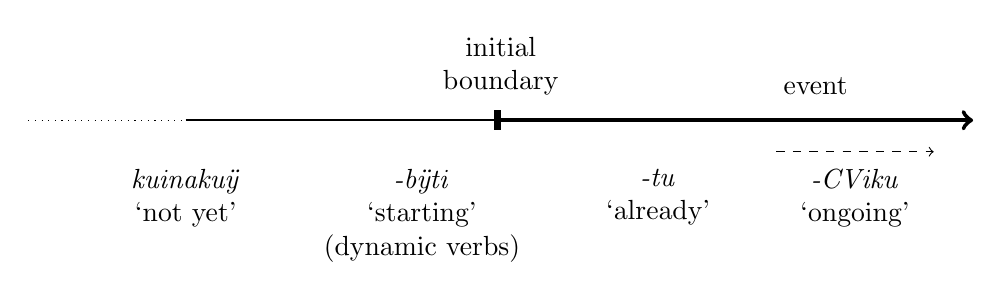
\begin{tikzpicture}
\draw[dotted] (-2,0)--(0,0);\draw [thick] [-|||]  (0,0) -- (4,0); \draw[ultra thick] [->]  (4,0) -- (10,0);
\draw[dashed][->] (7.5,-.4)--(9.5,-.4);
\node[align=center, above] at (4.0, .2){initial\\ boundary};%
\node[align=right, above] at (8.0, .2){event};%

\node[align=center, below] at (0.0,-.5)%
    {\textit{kuinakuÿ}\\‘not yet’};
\node[align=center, below] at (3.0,-.5)%
    {\textit{-bÿti}\\‘starting’\\(dynamic verbs)};
\node[align=center, below] at (6.0, -.5)%
    {\textit{-tu}\\‘already’ };
\node[align=center, below] at (8.5, -.5)%
    {\textit{-CViku}\\‘ongoing’ };
\end{tikzpicture}
\caption{Aspect markers acting on initial event boundaries}
\label{fig:AspectInitialBoundaries}
\end{figure}

\begin{figure}

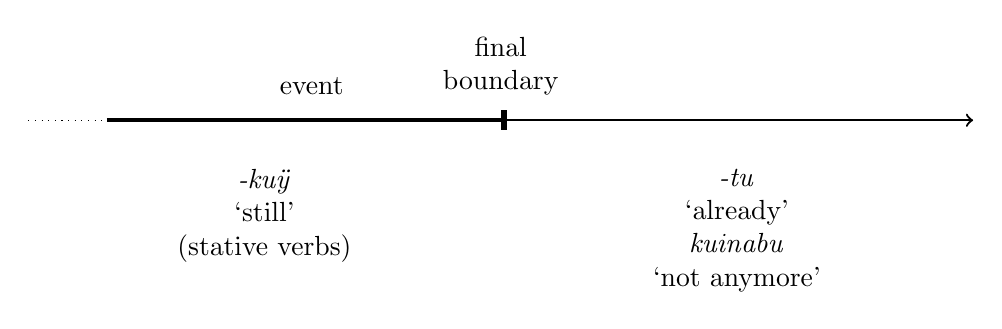
\begin{tikzpicture}
\draw[dotted] (-2,0)--(1,0);\draw [ultra thick] (-1,0) -- (4,0); \draw[thick] [|||->]  (4,0) -- (10,0);
\node[align=left, above] at (1.6, .2){event};%
\node[align=center, above] at (4.0, .2){final\\ boundary};%
\node[align=center, below] at (1.0,-.5)%
    {\textit{-kuÿ}\\‘still’\\(stative verbs)};

\node[align=center, below] at (7.0, -.5)%
    {\textit{-tu}\\‘already’\\\textit{kuinabu}\\‘not anymore’ };
\end{tikzpicture}
\caption{Aspect markers acting on final event boundaries}
\label{fig:AspectFinalBoundaries}
\end{figure}
\is{telicity|)}
\is{aktionsart|)}


\subsubsection{Iamitive perfect}\label{sec:Iamitive}\is{iamitive|(}

The most frequent of the tense and aspect markers of Paunaka is the omnipresent iamitive marker \textit{-tu}. The term “iamitive” is related to the better-known perfect. According to \citet[4]{Olsson2013}, iamitive markers are “aspectotemporal markers that seemingy [sic!] overlap with both the perfect and ‘already’”. Thus, a sentence like (\ref{ex:new23-dead}) can have various translations into English depending on the context.

\ea\label{ex:new23-dead}
\begingl
\glpreamble tipakutu\\
\gla ti-paku-tu\\
\glb 3i-die-\textsc{iam}\\
\glft ‘she is dead (already/now)’ \\or: ‘she has died (already/now)’
\endgl
%\trailingcitation{[]}
\xe

In his thesis, \citet[]{Olsson2013} described iamitives in some Southeast Asian languages in detail. Subsequently, \citet[]{DahlWalchli2016} proposed that the iamitive is a distinct gram type in a larger grammatical space that also includes perfects in the traditional sense and many other gram types that overlap in their uses. A new gram type, though with the name “new situation”, was also proposed by \citet[]{Ebert2001}, in analysing iamitive-like markers in Kiranti languages (reflected by the optional addition of “now” in the translation of (\ref{ex:new23-dead})).

Others have argued against gram status of the iamitive. Among them is \citet[]{Krajinovic2019}, who states that the differences from “traditional” perfects can still be explained within the functional realm of the perfect if we acknowledge that the perfect has distinct peculiarities in tenseless languages.\footnote{Actually, she identifies as a defining feature of perfects that they place the time the assertion is about (TT) posterior to the time the event took place (TSit) \citep[107]{Krajinovic2019}. However, this is not true for the Paunaka iamitive marker, which can also express that an event is currently ongoing.} I am agnostic as to the question whether the iamitive is a distinct gram type or should better be defined as a peculiar expression of the perfect gram or even be dismissed at all and be replaced by a more encompassing definition of perfect. I simply use the term “iamitive” here because the characteristics of the Paunaka marker fit relatively well the description of iamitive given by \citet[]{Olsson2013}. 

The iamitive is generally optional in Paunaka, in the sense that it does not enter into any obligatory binary distinction iamitive vs. non-iamitive, though its use is highly favoured in some situations. This should be kept in mind, when reading the following lines. 

According to \citet[4]{Olsson2013}, iamitives share with perfects the property of marking “the current relevance of a previous event”, but they differ from perfects in how they interact with the \isi{aktionsart} of a verb. This becomes apparent when considering stative verbs,\is{stative verb|(} since “certain types of states are particularly likely to be marked by iamitives, notably states that are the outcome of some natural process, such as ‘be ripe’ or ‘be grown up’” \citep[4]{Olsson2013}. Such states result from a “unidirectional development” of a “natural course of events” \citep[30]{Olsson2013}. This is exactly what we find in Paunaka. On stative predicates, the iamitive marker \textit{-tu} expresses, first, that the state holds at reference time, and second, that it is the result of some previous change,\is{resultative} i.e. that there existed a time prior to reference time in which the state did not hold. This is the main difference between an iamitive and a perfect, since the perfect does not imply that the state encoded by a stative verb currently holds \citep[cf.][9]{Olsson2013}.

The iamitive marker is \textit{-tu} in Paunaka and it is certainly related to the adverb \textit{metu} ‘ready, already’.

(\ref{ex:ripe-hair}) provides an example of a iamitive marker on a stative verb that encodes the result of a prior change of state, i.e. the hair colour of an elderly man, which has changed from black to grey or white, with the latter being expressed by the verb \textit{-yu} ‘be ripe’ in Paunaka. The example was elicited from Isidro.

\ea\label{ex:ripe-hair}
\begingl 
\glpreamble tiyutu nimukiji\\
\gla ti-yu-tu ni-muki-ji\\ 
\glb 3i-be.ripe-\textsc{iam} 1\textsc{sg}-hair-\textsc{col}\\ 
\glft ‘my hair is already white’
\trailingcitation{[mdx-c120416ls.150]}%semi-elicitated
\xe

In the same situation, Miguel proposed an answer containing the stative verb for ‘white, clear’, see (\ref{ex:white-hair}). However, this is not the way the colour of elderly people’s hair is usually referred to in Paunaka. All the same, the iamitive marker equally attaches to the verb here.

\ea\label{ex:white-hair}
\begingl
\glpreamble pisururutu\\
\gla pi-sururu-tu\\
\glb 2\textsc{sg}-be.clear-\textsc{iam}\\
\glft ‘you are already white’
\endgl
\trailingcitation{[mdx-c120416ls.143]}
\xe


(\ref{ex:nat-proc-yes-tu}) is about a ripe fruit and also builds on the verb \textit{-yu} ‘be ripe’. As in (\ref{ex:white-hair}) above, the iamitive marker is used on the verb. It also attaches to \textit{kana} ‘this size’, which is a \isi{demonstrative adjective} and thus we have an example of non-verbal predication here. The adjective is always accompanied by a gesture showing the actual size. The sentence comes from a correction session with María S. (it slightly differed from the one she had originally produced).

\ea\label{ex:nat-proc-yes-tu}
\begingl
\glpreamble kanainatu chÿi te tayutu binikatu\\
\gla kana-ina-tu chÿi te ti-a-yu-tu bi-nika-tu\\
\glb this.size-\textsc{irr.nv}-\textsc{iam} fruit \textsc{seq} 3i-\textsc{irr}-be.ripe-\textsc{iam} 1\textsc{pl}-eat.\textsc{irr}-\textsc{iam}\\
\glft ‘once the fruit has this size, then it is ripe and then we can eat it’
\endgl
\trailingcitation{[rxx-e121128s-3.11]}
\xe

Although it is highly common to attach a iamitive marker to a stative predicate that can be analysed as encoding the result of a process, this is not obligatory. In the following example, no iamitive is used on the verb \textit{-yu} ‘be ripe’, possibly because the change of state is backgrounded here, the more important information being the actual state of being ripe as a precondition for the chicken eating the fruit. %It is thus excluded that the stative verb \textit{-yu} ‘be ripe’ is not a stative verb at all but an inchoative verb.
The sentence comes from María S., too.

\ea\label{ex:nat-proc-no-tu}
\begingl 
\glpreamble kuina chinijanea, kuina, abÿrÿsÿi si kue tayu chinijanea\\
\gla kuina chi-ni-jane-a kuina abÿrÿsÿi si kue ti-a-yu chi-ni-jane-a\\ 
\glb \textsc{neg} 3-eat-\textsc{distr}-\textsc{irr} \textsc{neg} guava yes if 3i-\textsc{irr}-be.ripe 3-eat-\textsc{distr}-\textsc{irr}\\ 
\glft ‘they (the chicken) don’t eat it, no, guavas, yes, they eat if they are ripe’
\trailingcitation{[rxx-e121126s-3.36]}
\xe

If the stative verb does not encode the endpoint of a natural development per se, then such a reading is added by the iamitive marker.\is{stative verb|)}  It can, for example, combine with the non-verbal existential \isi{copula} \textit{kaku}, and in this case, it expresses that something has come into existence by reference time that has not been there before. This can be seen in the following example (\ref{ex:ticks}).

The context is as follows: Miguel and I had paid José a visit and when we came back to the village, we were bitten by some small ticks. Miguel made a comment that there were many ticks, and María S. reacted with a question, which can rather be read as an expression of surprise than as a request for information. Apparently, she was surprised that the tick season had already started, since she had not noticed any ticks up to this point.

\ea\label{ex:ticks}
\begingl 
\glpreamble ¿kakutu samuchu?\\
\gla kaku-tu samuchu\\ 
\glb exist-\textsc{iam} tick.sp\\ 
\glft ‘there are ticks already?’
\trailingcitation{[mrx-c120509l.149]}
\xe

Another case in which the iamitive adds a development reading to a stative predicate, but this time a verbal one, is (\ref{ex:know-cos}). Together with the iamitive marker, the verb \textit{-(i)chuna} ‘know, be capable, be able’ encodes that knowledge has been acquired by learning. However, the focus still lies on the state after the process of learning and not on the process itself.

In this example, Juana talks about her grandson.

\ea\label{ex:know-cos}
\begingl 
\glpreamble tijÿku i netuku xhikuera i tichunatu te i tiyunu kuarterayae...\\
\gla ti-jÿku i nÿ-etuku xhikuera i ti-ichuna-tu te i ti-yunu kuartera-yae\\ 
\glb 3i-grow and 1\textsc{sg}-put school and 3i-be.capable-\textsc{iam} \textsc{seq} and 3i-go military.base-\textsc{loc}\\ 
\glft ‘he grew and I put him into school and once he had acquired knowledge (i.e. learned), then he went to the military base...’
\trailingcitation{[jxx-p110923l-1.173-176]}
\xe

Finally, the iamitive also appears on nouns denoting high age, when they are used as a predicate,\is{nominal predicate} but not if they are an argument of the clause. Compare (\ref{ex:old-woman-2}), where \textit{juberÿpu\-nÿtu} ‘I am an old woman’ is the predicate, with (\ref{ex:old-woman-1}), in which \textit{juberÿpu\-mÿnÿ} ‘dear old woman’ is the object of the clause and thus bears no iamitive marker.


(\ref{ex:old-woman-2}) is a statement by María C. about herself.

\ea\label{ex:old-woman-2}
\begingl 
\glpreamble juberÿpunÿtu kuina puero trabakuinabu\\
\gla juberÿpu-nÿ-tu kuina puero trabaku-ina-bu\\ 
\glb old.woman-1\textsc{sg}-\textsc{iam} \textsc{neg} can work-\textsc{irr.nv}-\textsc{dsc}\\ 
\glft ‘I am old, I cannot work anymore’
\trailingcitation{[uxx-p110825l.203]}
\xe

In (\ref{ex:old-woman-1}), Juana talks about the chance she once had to go to Europe to work there. In the end, she did not go; this is why the frustrative is used here.

\ea\label{ex:old-woman-1}
\begingl 
\glpreamble niyunaini nichenenaikupa juberÿpumÿnÿ\\
\gla ni-yuna-ini ni-chenenaiku-pa juberÿpu-mÿnÿ\\ 
\glb 1\textsc{sg}-go.\textsc{irr}-\textsc{frust} 1\textsc{sg}-care.for-\textsc{dloc.irr} old.woman-\textsc{dim}\\ 
\glft ‘I would have gone (to Austria) to care for an old woman’
\trailingcitation{[jxx-e120516l-1.015]}
\xe


Considering dynamic verbs, we can distinguish between telic and atelic\is{telicity|(} predicates.\is{aktionsart|(} \citet[19]{Olsson2013} predicts that “[w]ith a telic predicate, the ‘new situation’ asserted by the iamitive corresponds to the situation following the final boundary (or, with an achievement, following the only boundary)”. In combination with atelic verbs, however, the action can either be finished or ongoing. This is because “a iamitive can be interpreted as applying either to the initial boundary, thus yielding an on-going interpretation, or to the final boundary, yielding a completed, ‘past’ interpretation” \citep[19]{Olsson2013}. 

Let us first consider some telic verbs. First of all, the iamitive marker can encode a state resulting from an event as in (\ref{ex:die-iam}).\is{resultative}

The sentence comes from Juana telling the story about the fox and the jaguar. At this point of the story, the jaguar has been dead for several months already, and the fox comes back to the pond where he died to spitefully speak with his skeleton. The fox starts in Spanish, but continues the sentence in Paunaka.\footnote{The Spanish phrase \textit{¿no ve?} is not to be understood literally (‘he/she doesn’t see’). In Bolivia, it is used as a tag question to seek confirmation similar to English ‘right?’ or ‘you know?’ \citep[45]{Mendoza2015}.}

\ea\label{ex:die-iam}
\begingl
\glpreamble “¿no ve? tío, ¡pipakutu!”\\
\gla {no ve} tío pi-paku-tu\\
\glb {right} uncle 2\textsc{sg}-die-\textsc{iam}\\
\glft ‘“right, uncle? you’re dead!”’
\endgl
\trailingcitation{[jmx-n120429ls-x5.286-287]}
\xe

The fact that there is a state resulting from a punctual event is not enough to trigger iamitive marking, though. There is a complex interplay between aktionsart\is{aktionsart|)} of the verb, \isi{reality status}, derivational morphology and also middle voice\is{middle voice|(}. Middle verbs often imply a continuous state, and thus \textit{-tupunu-bu} ‘arrive’ already implies a \isi{resultative} state as opposed to the punctual \textit{-tupunu} ‘reach’; see (\ref{ex:arrive-no-iam}), where we need a perfect in the English translation, but no iamitive in the original Paunaka sentence. The same is true for the middle verb \textit{-yÿtiku-bu} ‘cook’, which relates to \textit{-yÿtiku} ‘set (a pot) on fire’ and for all posture verbs.

(\ref{ex:arrive-no-iam}) was elicited from María S.

\ea\label{ex:arrive-no-iam}
\begingl
\glpreamble chuinepaiku titupunubu nichechapÿi\\
\gla uchuine-paiku ti-tupunubu ni-chechapÿi\\
\glb just.now-\textsc{punct} 3i-arrive 1\textsc{sg}-son \\
\glft ‘my son has just arrived’
\endgl
\trailingcitation{[rxx-e181022le.124]}
\xe
\is{middle voice|)}

If \textit{-tupunubu} ‘arrive’ is combined with a iamitive, it rather evokes anteriority or earliness readings or it expresses that an expectation is fulfilled, which is just what we expect from a iamitive \citep[cf.][21]{Olsson2013}. Prior to (\ref{ex:arrive-iam}), María S. had told me that Federico and Swintha had already informed her that I would come to Bolivia.

\ea\label{ex:arrive-iam}
\begingl
\glpreamble jaa metu pitupunubutu naka\\
\gla jaa metu pi-tupunubu-tu naka\\
\glb \textsc{afm} already 2\textsc{sg}-arrive-\textsc{iam} here\\
\glft ‘yes, and now you have arrived here’
\endgl
\trailingcitation{[rxx-e181017l.005]}
\xe

In (\ref{ex:arrive-iam}), the iamitive combines with the adverb \textit{metu} ‘already, ready’ to indicate current relevance. In (\ref{ex:broken-iam}) on the other hand, \textit{metu} and the iamitive-marked verb indicate earliness of a resultative state. The example was elicited from María S. and corresponds to an invented situation, in which a mother asks her daughter who may have broken a pot, and the daughter answers that she doesn’t know and that the pot was already broken, when she saw it. Note that the iamitive marker also occurs on the first atelic verb \textit{-imu} ‘see’ here.

\ea\label{ex:broken-iam}
\begingl
\glpreamble nimutu metu terabajikutu\\
\gla ni-imu-tu metu ti-rabajiku-tu\\
\glb 1\textsc{sg}-see-\textsc{iam} already 3i-break-\textsc{iam}\\
\glft ‘when I saw it, it was already broken’
\endgl
\trailingcitation{[rxx-e181021les.222]}
\xe

Current relevance is also at work in (\ref{ex:stuck}), where use of the iamitive indicates that the result of the dog’s sticking its head into the glass (or pot) is of importance. The example comes from Miguel telling José the \isi{frog story}. The fact that the dog’s head got stuck was expressed lexically in the sentence that followed. 

\ea\label{ex:stuck}
\begingl
\glpreamble i naka chipurutukutu eka kabe chichÿti naka eka tachukÿyae\\
\gla i naka chi-purutuku-tu eka kabe chi-chÿti naka eka tachu-kÿ-yae\\
\glb and here 3-put.in-\textsc{iam} \textsc{dem}a dog 3-head here \textsc{dem}a small.pot-\textsc{clf}:bounded-\textsc{loc}\\
\glft ‘and here the dog has stuck his head into the small pot here’
\endgl
\trailingcitation{[mox-a110920l-2.052]}
\xe

So far, we have only looked at telic verbs with \isi{realis} RS. It is also possible to combine an \isi{irrealis} verb with iamitive. Irrealis, among other things, can express \isi{future reference} of an event. Combination with the iamitive can then indicate that the final boundary has not yet been reached although the measures have been taken to reach it. This is the case in (\ref{ex:breed-iam}), where the final boundary is the hatching of the chicken. The sentence was elicited from Juana, who had just told me that her hen was breeding.

\ea\label{ex:breed-iam}
\begingl
\glpreamble tipuichakatu takÿrajanemÿnÿ\\
\gla ti-puichaka-tu takÿra-jane-mÿnÿ\\
\glb 3i-hatch.\textsc{irr}-\textsc{iam} chicken-\textsc{distr}-\textsc{dim}\\
\glft ‘it will hatch eggs (lit.: little chicken)’
\endgl
\trailingcitation{[jxx-e110923l-2.086]}
\xe

Atelic\is{aktionsart|(} verbs with a iamitive marker can be interpreted as encoding either an ongoing or a completed action as is predicted by \citet[19]{Olsson2013}, because the iamitive can apply to either the initial or the final boundary of the event. Thus in an invented situation, in which a mother invites her son to eat something, the answer including the iamitive can either mean that the son has already eaten or that he is eating at that very moment (and the mother does not see him because he is sitting behind the house), see (\ref{ex:atelic-iam}). 

\ea\label{ex:atelic-iam}
\begingl
\glpreamble nÿnikutu\\
\gla nÿ-niku-tu\\
\glb 1\textsc{sg}-eat-\textsc{iam}\\
\glft ‘I am already eating’\\ or: ‘I have eaten already’
\endgl
\trailingcitation{[rxx-e181021les.202, 205]}
\xe
\is{aktionsart|)}

Equally, if the mother asks her son to send her daughter to go and fetch water, the answer including the iamitive can either indicate that the daughter has completed the task or is busy on the task at that very moment, as in (\ref{ex:atelic-iam-2}), which was also elicited from María S.

\ea\label{ex:atelic-iam-2}
\begingl
\glpreamble tiyunutu tepa ÿne\\
\gla ti-yunu-tu ti-epa ÿne\\
\glb 3i-go-\textsc{iam} 3i-take.\textsc{irr} water\\
\glft ‘she is already going to fetch water’\\or: ‘she already went to fetch water’
\endgl
\trailingcitation{[rxx-e181022le]}
\xe
\is{telicity|)}

However, if it is necessary to clarify that the action is taking place right now, speakers can also resort to continuous\is{continuous|(} marking (see \sectref{sec:ActiveVerbs_RDPL}). They can then add the iamitive to the continuous verb. Additionally, an adverb can help to clarify temporal reference. Both strategies are combined in (\ref{ex:atelic-cont-iam}), which was elicited from Juana, providing her with the same invented context as María S. in (\ref{ex:atelic-iam}) above.

\ea\label{ex:atelic-cont-iam}
\begingl
\glpreamble ¡ninikutu mimi! ninikukuikutu tanÿma naka\\
\gla ni-niku-tu mimi ni-niku-kuiku-tu tanÿma naka\\
\glb 1\textsc{sg}-eat-\textsc{iam} mum 1\textsc{sg}-eat-\textsc{cont}-\textsc{iam} now here\\
\glft ‘I am already eating, mum! I am already eating here right now’
\endgl
\trailingcitation{[jxx-e181104l-3]}
\xe
\is{continuous|)}

The following two examples were produced more spontaneously, and we can notice that the iamitive marker on one and the same verb, \textit{-kutijiku} ‘escape, flee’, can express that the action, i.e. the escape, is successfully completed as in (\ref{ex:iam-flee-1}), or ongoing as in (\ref{ex:iam-flee-2}).

In (\ref{ex:iam-flee-1}), Juana tells me about a criminal in-law of hers who had hidden away in the woods. When he was detected, some people went to the woods in search of him, but he had managed to escape before.

\ea\label{ex:iam-flee-1}
\begingl
\glpreamble kuina kakuinabu nauku kimenubu, tikutijikutu\\
\gla kuina kaku-ina-bu nauku kimenu-bu ti-kutijiku-tu\\
\glb \textsc{neg} exist-\textsc{irr.nv}-\textsc{dsc} there woods-\textsc{dsc} 3i-flee-\textsc{iam}\\
\glft ‘he wasn’t there anymore in the woods, he had escaped’
\endgl
\trailingcitation{[jxx-p120430l-2.053]}
\xe

(\ref{ex:iam-flee-2}) refers to the picture in the \isi{frog story} in which the dog is running away from the bees. Its escape is thus ongoing. The example comes from Miguel.

\ea\label{ex:iam-flee-2}
\begingl
\glpreamble chijikiu eka kabe tikutijikutu i eka janejane cheikukuiku\\
\gla chijikiu eka kabe ti-kutijiku-tu i eka jane-jane chÿ-eikukuiku\\
\glb however \textsc{dem}a dog 3i-flee-\textsc{iam} and \textsc{dem}a wasp-\textsc{distr} 3-chase\\
\glft ‘nonetheless, the dog is fleeing and the wasps are chasing it’
\endgl
\trailingcitation{[mox-a110920l-2.104]}
\xe

Two more examples with telic verbs follow. In (\ref{ex:iam-atel-1}) by Miguel, the initial boundary of the action is triggered (or established) by the iamitive. The sentence provides the funny climax of one of the episodes of the story of the fox and the jaguar. The jaguar has caught a vulture and wants to eat him, and the vulture seemingly surrenders and proposes that the jaguar plucks him except for his wings and throws him up into the air so that he would fall down back into his open mouth. The jaguar obeys, but instead of falling, the vulture defecates into the jaguar’s mouth and then flies away. It is thus the initial boundary of flying, the take-off, that is important in (\ref{ex:iam-atel-1}).

\ea\label{ex:iam-atel-1}
\begingl
\glpreamble i te tibÿbÿkutuji echÿu sÿmÿ tiyunu\\
\gla i te ti-bÿbÿku-tu-ji echÿu sÿmÿ ti-yunu\\
\glb and \textsc{seq} 3i-fly-\textsc{iam}-\textsc{rprt} \textsc{dem}a vulture 3i-go\\
\glft ‘and then the vulture flew off, it is said, and went (i.e. escaped)’
\endgl
\trailingcitation{[jmx-n120429ls-x5.211]}
\xe

In (\ref{ex:iam-atel-3}), the atelic verb\is{telicity} \textit{-pajÿku} ‘stay’ is turned into a non-reversed or even irreversible state (‘have stayed ever since, stay for good’) by addition of the iamitive. The example also comes from the story of the fox and the jaguar, but this time is narrated by María S. on another occasion. It is the jaguar who – tricked by the fox – jumps into the water and drowns. 

\ea\label{ex:iam-atel-3}
\begingl
\glpreamble tijipaikuji ÿneji te tepajÿkutu ÿneyae\\
\gla ti-jipaiku-ji ÿne-ji te ti-pajÿku-tu ÿne-yae\\
\glb 3i-jump.down-\textsc{rprt} water-\textsc{rprt} \textsc{seq} 3i-stay-\textsc{iam} water-\textsc{loc}\\
\glft ‘he jumped into the water and then he stayed in the water for good, it is said’
\endgl
\trailingcitation{[rxx-n120511l-1.039]}
\xe


(\ref{ex:iam-flee-1})--(\ref{ex:iam-atel-3}) all consist of two combined clauses,\is{complex sentence|(} but the iamitive is only marked once – an exception possibly being (\ref{ex:iam-flee-1}), whose first clause is marked for discontinuous, a category related to the iamitive, see \sectref{sec:Discontinuous} below. \citet[39]{Olsson2013} found that in clause combining, iamitives are often used to indicate temporal sequentiality. In all the examples he gives in his work, the iamitive appears in a clause that expresses the temporally anterior event. As for Paunaka, there are some examples that seem to verify this analysis, while others contradict it. Consider (\ref{ex:predicate1}) and (\ref{ex:predicate2-te}). In the first of them, the first event in the sequence is marked, in the second one it is the second event that receives iamitive aspect. 
Note that both clauses have irrealis RS for different reasons: (\ref{ex:predicate1}) is from a general description of how to use a clay pot, while (\ref{ex:predicate2-te}) has a habitual past reading. Both sentences are about usage of a clay pot and both come from Juana.

\ea\label{ex:predicate1}
\begingl 
\glpreamble tibururukatu ÿne i pijuka\\
\gla ti-bururuka-tu ÿne i pi-juka\\ 
\glb 3i-boil.\textsc{irr}-\textsc{iam} water and 2\textsc{sg}-pour.solid.\textsc{irr}\\ 
\glft ‘the water boils (now) and you pour it (i.e. the food) in’
\trailingcitation{[jxx-d110923l-3]}
\xe

\ea\label{ex:predicate2-te}
\begingl 
\glpreamble taima te binikatu\\
\gla ti-a-ima te bi-nika-tu\\ 
\glb 3i-\textsc{irr}-be.cooked \textsc{seq} 1\textsc{pl}-eat.\textsc{irr}-\textsc{iam}\\ 
\glft ‘when it was done, then we would/could eat it (i.e. the food)’
\trailingcitation{[jxx-d110923l-2.25]}
\xe

In both examples above, the iamitive could have probably also been attached to the other clause instead or additionally. Recall that \citet[]{Ebert2001} speaks of importance of a new situation, and \citet[9]{Olsson2013} notes that iamitives are often translated with “now”. Just like the English word “now” could mark either of the two events in (\ref{ex:predicate1}) and (\ref{ex:predicate2-te}) (ignoring for a moment the fact that “now” is not compatible with habitual contexts at all), the iamitive is possible on both predicates. This is because being optional the iamitive does not encode any absolute properties of the event’s tempo-aspectual setting, but simply signals what the speaker finds worth being marked as the new situation. In (\ref{ex:predicate1}), the iamitive is encodes that event 1 has to be realised in order for event 2 to be possible or appropriate. In (\ref{ex:predicate2-te}), however, the function of the iamitive is to close the statement \citep[cf.][8]{Olsson2013}. The use of the iamitive thus signals that the discourse topic is completed and we can expect a switch to another topic or another (discourse) aspect of the topic. We often find an iamitive on the last predicate of a chain of clauses which all provide information to the same overarching discourse topic.\is{complex sentence|)} 

(\ref{ex:predicate2}) provides another example of the use of \textit{-tu} in a clause that closes the description of a sequence of events. It was produced by Juana, after she had found loam for her clay pot in order to give us a description of what she would do now. Following the sentence in (\ref{ex:predicate2}), she talked about bringing the loam to her house and resume the production of the pot there, so there is a change of location, a new, separate step in the development of her pot, anticipated by the use of the iamitive here.

\ea\label{ex:predicate2}
\begingl 
\glpreamble betuku naka bichÿtiyae i biyunatu\\
\gla bi-etuku naka bi-chÿti-yae i bi-yuna-tu\\ 
\glb 1\textsc{pl}-put here 1\textsc{pl}-head-\textsc{loc} and 1\textsc{pl}-go.\textsc{irr}-\textsc{iam}\\ 
\glft ‘we put it (the bag) here on our head and we can go (now)’
\trailingcitation{[jmx-d110918ls-2.02-03]}
\xe

It should have become clear by now that the iamitive has a wide range of different functions, and since it is so multifunctional, it is no surprise that it is used very frequently. We often find the iamitive on states that result\is{resultative} from a previous unidirectional development, we find it with completed and ongoing actions, and we find it in clause combining,\is{complex sentence} often together with the \isi{sequential} \isi{connective} \textit{te} ‘then’ and with the adverb \textit{metu} ‘already, ready’ as well as borrowed forms of the Spanish adverb \textit{después} ‘after’ (borrowed as e.g. \textit{depue}, \textit{repue}). However, there is one context in which we do not find the iamitive: \isi{negation}.\footnote{There are a handful of examples in the corpus in which the iamitive is found in a negative clause, but they are so few that they should probably be treated as mistakes.} 

Cross-linguistically, iamitives often combine with negation and then they usually exhibit either a discontinuative meaning or a meaning described as ‘not yet/still not’ \citep[cf.][35--36]{Olsson2013}. Paunaka  has separate aspect markers for the \isi{discontinuous} and the \isi{incompletive} (the latter being the term chosen here for the meaning of ‘not yet’ and its positive counterpart ‘still’). The iamitive marker is usually not found in negative clauses\is{negation} with one exception: If the \isi{negative particle} \textit{kuina} is the predicate itself, \textit{-tu} can be added after the \isi{discontinuous} marker to emphasise that the negative state that is contrasted to the anterior positive state holds at reference time, see (\ref{ex:kuinabutu}). The sentence comes from María S. telling the story about the two hunters and the devil. This is what one of the men tells the devil after the latter has eaten up everything the two men had hunted.

 \ea\label{ex:kuinabutu}
\begingl
\glpreamble “kuinabutu chija nenikapi”\\
\gla kuina-bu-tu chija nÿ-nika-pi\\
\glb \textsc{neg}-\textsc{dsc}-\textsc{iam} what 1\textsc{sg}-feed.\textsc{irr}-2\textsc{sg}\\
\glft ‘“there isn’t anything left that I could give you to eat”’
\endgl
\trailingcitation{[rxx-n120511l-2.45-46]}
\xe

The following sections provide information about aspects related to the iamitive, discontinuous aspect is described in \sectref{sec:Discontinuous} and incompletive aspect in \sectref{sec:Incompletive}.\is{iamitive|)} 


\subsubsection{Discontinuous}\label{sec:Discontinuous}\is{discontinuous|(}
\is{negation|(}
The discontinuous marker \textit{-bu} is exclusively used in negative clauses and can be translated with ‘anymore’. It expresses that a state does not hold any longer or that an action is not performed anymore. It thus targets a final boundary, but unlike the English adverb, it seems to imply the state after the final boundary most of the times rather than focus on the final boundary itself, so \textit{kuina x-bu} means ‘after x, be in a state of not-x’ rather than ‘x is over (thus y)’. To demonstrate this, consider the following English sentences, which all include the adverb \textit{anymore}.

\begin{enumerate}
\item He does not eat anymore (because he is ill).\label{item:dsc-1}
\item He won’t eat anymore today (because he has eaten so much).\label{item:dsc-2}
\item He  isn’t eating anymore (so you can talk to him now).\label{item:dsc-3}
\end{enumerate}

The discontinuous marker predominantly occurs in contexts similar to \ref{item:dsc-1}. (state ‘no-x after x’ has a long duration or is persistent), and contexts like \ref{item:dsc-2}. (state ‘no-x after x’ has a limited duration) have also been found. However, as for \ref{item:dsc-3}. (state ‘no-x’ corresponds to end of x), there are only very few examples that could be analysed as corresponding to similar contexts. 
 
The discontinuous marker can either attach to the predicate or to the negative particle or to both with no apparent difference in meaning. Consider (\ref{ex:DSCnew-1}). There are two juxtaposed clauses: in the first one the marker attaches to the verb and in the second one to the negative particle. It comes from Juana who was talking about the making of the reservoir in Santa Rita. Once it was ready, people from Santa Rita did not have to walk far anymore to get water.

\ea\label{ex:DSCnew-1}
\begingl
\glpreamble kuina biyunabu Naranjito, kuinabu biyuna naka Tavistayae\\
\gla kuina bi-yuna-bu Naranjito kuina-bu bi-yuna naka Tavista-yae\\
\glb \textsc{neg} 1\textsc{pl}-go.\textsc{irr}-\textsc{dsc} Naranjito \textsc{neg}-\textsc{dsc} 1\textsc{pl}-go.\textsc{irr} here Altavista-\textsc{loc}\\
\glft ‘we don’t have to go to Naranjito anymore, we don’t have to go to \isi{Altavista} anymore’
\endgl
\trailingcitation{[jxx-p120515l-2.207-208]}
\xe

An example in which \textit{-bu} attaches to both negative particle and predicate is (\ref{ex:dsc-1}). It is a statement by María C. about her ability to see, which has decreased over time, since she is an old lady.

\ea\label{ex:dsc-1}
\begingl 
\glpreamble kuinabu naimubÿkebu\\
\gla kuina-bu nÿ-a-imubÿke-bu\\ 
\glb \textsc{neg}-\textsc{dsc} 1\textsc{sg}-\textsc{irr}-see.well-\textsc{dsc}\\ 
\glft ‘I can’t see well anymore’
\trailingcitation{[uxx-p110825l.013]}
\xe

%In negative existential sentences, there is often no separate predicate to which the discontinuous marker could attach, the negative particle being the predicate itself. This is the case in: kakukuÿnube echÿu paunakanube o kuinabunubetu, ump-p110815sf.127

Although the discontinuous marker and the middle marker\is{middle voice} are homophonous, they cannot be confused. The middle marker has an allophone \textit{-pu} that occurs after \isi{irrealis}. The predicates to which the discontinuous marker attaches necessarily have \isi{irrealis} RS, since they are all negated, and the form of the discontinuous marker is always \textit{-bu}. An example in which both markers co-occur has already been given in \sectref{sec:Middle_voice} (ex. (\ref{ex:MID-DSC})).

A few more examples of the discontinuous marker shall be given here.

(\ref{ex:dsc-3}) was produced by Juana, when I was visiting her in Santa Cruz, where she was living at that time. She uttered the assumption that I would not go back to Concepción from Santa Cruz, but rather stay there in order to leave for Germany directly (which was not the case, since I had indeed planned to spend a few more days in Concepción before coming back to Santa Cruz and subsequently travel back to Germany).

\ea\label{ex:dsc-3}
\begingl 
\glpreamble kuina piyunupunabu Concecionyae\\
\gla kuina pi-yunupuna-bu Concecion-yae\\ 
\glb \textsc{neg} 2\textsc{sg}-go.back.\textsc{irr}-\textsc{dsc} Concepción-\textsc{loc}\\ 
\glft ‘you won’t go back to Concepción anymore’
\trailingcitation{[jxx-p120430l-1.134]}
\xe

%In (\ref{ex:dsc-4}) the discontinuous marker is found on a non-verbal predicate.\footnote{Note that verbs from Spanish are often borrowed as non-verbal predicates, see \sectref{sec:borrowed_verbs}.} The sentence is from the account of the Paunaka history given by Miguel and presents the reason why the first inhabitant of Santa Rita was allowed to move away from Altavista to found a new village.
%
%\ea\label{ex:dsc-4}
%\begingl 
%\glpreamble kuina pueroinabu trabakuinabu chitÿpi echÿu patron\\
%\gla kuina puero-ina-bu trabaku-ina-bu chi-tÿpi echÿu patron\\ 
%\glb \textsc{neg} can-\textsc{irr.nv}-\textsc{dsc} work-\textsc{irr.nv}-\textsc{dsc} 3-\textsc{ben} \textsc{dem}b boss\\ 
%\glft ‘he couldn’t work for the \textit{patrón} anymore’\\ 
%\endgl
%\trailingcitation{[mxx-p110825l.024-025]}
%\xe

(\ref{ex:DSCnew-4}) has a nominal predicate. Miguel speaks of a village close to Santa Rita which was abandoned.

\ea\label{ex:DSCnew-4}
\begingl
\glpreamble kuinabutu jentenubeinabu nauku\\
\gla kuina-bu-tu jente-nube-ina-bu nauku\\
\glb \textsc{neg}-\textsc{dsc}-\textsc{iam} man-\textsc{pl}-\textsc{irr.nv}-\textsc{dsc} there\\
\glft ‘there are no people anymore there now’
\endgl
\trailingcitation{[mty-p110906l.134]}
\xe

(\ref{ex:DSCnew-1})–(\ref{ex:DSCnew-4}) above all refer to persistent states resulting from the termination of an event x. As has been stated in the introduction to this section, this is the most typical usage of the discontinuous marker. In the following two examples, however, \textit{-bu} is used to refer to easily reversible states or states of a limited duration.

In (\ref{ex:DSCnew-5}), Juana speaks about the weather after there was heavy rainfall the day before. Following this statement, she mentioned that the forecast had announced rainfall for the next day, so the state definitely has no long duration. Note that Juana uses the adverb \textit{metu} to encode exactly this short duration.

\ea\label{ex:DSCnew-5}
\begingl
\glpreamble pero metu kuina tikebabu\\
\gla pero metu kuina ti-keba-bu\\
\glb but already \textsc{neg} 3i-rain.\textsc{irr}-\textsc{dsc}\\
\glft ‘but for now it is not going to rain anymore’
\endgl
\trailingcitation{[jxx-e120516l-1.101]}
\xe


In (\ref{ex:dsc-5}), María C. is speaking about the scarceness of corn. As a consequence, she will soon not be able to drink chicha, a drink made from corn, but has to drink water. The state is reversible because as soon as she gets some money, María C. can buy more corn and make chicha again (i.e. the shortage is not due to crop failure in this case; due to her advanced age, the speaker did not have a field anymore at that time).

\ea\label{ex:dsc-5}
\begingl
\glpreamble kakumÿnÿ amukemÿnÿ te tibukapu echÿu te kuinabu nea aumue\\
\gla kaku-mÿnÿ amuke-mÿnÿ te ti-buka-pu echÿu te kuina-bu nÿ-ea aumue\\
\glb exist-\textsc{dim} corn-\textsc{dim} \textsc{seq} 3i-finish.\textsc{irr}-\textsc{mid} \textsc{dem}b \textsc{seq} \textsc{neg}-\textsc{dsc} 1\textsc{sg}-drink.\textsc{irr} chicha\\
\glft ‘there is little corn and when it is finished, then I cannot drink chicha anymore’
\endgl
\trailingcitation{[ump-p110815sf.693]}
\xe

Finally, the last two examples given here demonstrate a possible use of the marker that targets the end of an event rather than the state after it. One of them is (\ref{ex:DSCnew-3}), which was elicited from María S. providing her with the context that somebody is lying in a hammock.

\ea\label{ex:DSCnew-3}
\begingl
\glpreamble kuina timukabu\\
\gla kuina ti-muka-bu\\
\glb \textsc{neg} 3i-sleep.\textsc{irr}-\textsc{dsc}\\
\glft ‘she is not sleeping anymore’
\endgl
\trailingcitation{[rxx-e181024l]}
\xe

Another example that possibly targets the end of an event is (\ref{ex:DSCnew-2}), but it cannot be excluded that it refers to a reversible state after the event. The sentence was produced by María S. when some piglets had shown up at her yard grunting, but then suddenly got quiet because they started to suckle at their mother’s teats. Now, it is not clear whether María S. was referring to the stopping of grunting at that very moment or the fact that the piglets would stop grunting for a while, since they were not hungry anymore.

\ea\label{ex:DSCnew-2}
\begingl
\glpreamble tujijaneutu, nechikue kuina tasabaibujane\\
\gla ti-uji-jane-u-tu nechikue kuina ti-a-sabai-bu-jane\\
\glb 3i-suckle-\textsc{distr}-\textsc{real}-\textsc{iam} therefore \textsc{neg} 3i-\textsc{irr}-shout-\textsc{dsc}-\textsc{distr}\\
\glft ‘they are suckling now, thus they are not grunting anymore’\\or: ‘..., thus they do not grunt anymore’
\endgl
\trailingcitation{[rmx-e150922l.155-156]}
\xe
\is{negation|)}
\is{discontinuous|)}


\subsubsection{Incompletive}\label{sec:Incompletive}\is{incompletive|(}

Unlike the \isi{iamitive} (see \sectref{sec:Iamitive}) and the \isi{discontinuous} marker (see \sectref{sec:Discontinuous}), the incompletive marker \textit{-kuÿ} ‘still, (not) yet’ can occur in positive and in negative sentences. It marks an event as ongoing at reference time, while simultaneously implying the termination of the event at a later point in time.

In positive sentences, \textit{-kuÿ} is found on predicates denoting reversible states. It always has stative overtones, even if the verb is active\is{active verb}. It would not be used in a sentence corresponding to ‘He is still eating (you cannot talk to him right now)’, i.e. it is not compatible with a progressive interpretation of an action.

While the \isi{iamitive} is found on states that mark the outcome of a “natural course of events” \citep[30]{Olsson2013}, the incompletive is typically used with words denoting the starting point of such a development, usually nouns denoting young age, and sometimes also verbs that are used to illustrate young age, which means they are not understood actively but statively in these cases. In (\ref{ex:INCMPL-5}), we find the incompletive marker being attached to a noun, in (\ref{ex:INCMPL-4}) to an adjective, and in (\ref{ex:INCMPL-3}) to an adjective and to a verb.

(\ref{ex:INCMPL-5}) was produced by Miguel, when talking about the old days with Juan C. I do not know what exactly this sentence refers to, because I did not understand the previous sentences, but it has to do with the behaviour of \textit{karay} towards the people in Santa Rita.

\newpage
\ea\label{ex:INCMPL-5}
\begingl 
\glpreamble i nÿti nikechu: “kuina pueroina, pue nÿti aitubuchepÿikuÿni”\\
\gla i nÿti ni-kechu kuina puero-ina pue nÿti aitubuchepÿi-kuÿ-ni\\ 
\glb and 1\textsc{sg.prn} 1\textsc{sg}-say \textsc{neg} can-\textsc{irr.nv} well 1\textsc{sg.prn} boy-\textsc{incmp}-1\textsc{sg}\\ 
\glft ‘and I said: “I can’t, I am still a young man”’
\trailingcitation{[mqx-p110826l.386]}
\xe

In (\ref{ex:INCMPL-4}) the incompletive marker attaches to the \isi{demonstrative adjective} \textit{kana} ‘be of this size’. The sentence comes from María C. in telling about the hard childhood and youth she had.

\ea\label{ex:INCMPL-4}
\begingl
\glpreamble kanakuÿnemÿnÿni tepaku nÿa ja\\
\gla kana-kuÿ-ne-mÿnÿ-ni ti-paku nÿ-a ja\\
\glb this.size-\textsc{incmp}-1\textsc{sg}-\textsc{dim}-\textsc{deict} 3i-die 1\textsc{sg}-father \textsc{afm}\\
\glft ‘when I still was this size (showing with hands), my father died’
\endgl
\trailingcitation{[ump-p110815sf.149]}
\xe


If the incompletive marker combines with active verbs,\is{active verb|(} they normally express a state rather than an action. In (\ref{ex:INCMPL-3}), the marker is found on a nominal predicate first and then on an active verb; however, this does not mean that the action is going on at that very moment, but rather that the referents are in a state in which the action is still being carried out appropriately. It refers to some puppies that were running around in the yard of María S. and were apparently very hungry. Somebody had brought them to Santa Rita from Concepción, although they were still much too small to survive without being fed by their mother.

\ea\label{ex:INCMPL-3}
\begingl 
\glpreamble hmm, sepitÿkuÿjaneyu tujikukuÿjaneyu\\
\gla hmm sepitÿ-kuÿ-jane-yu ti-ujiku-kuÿ-jane-yu\\ 
\glb \textsc{intj} small-\textsc{incmp}-\textsc{distr}-\textsc{ints} 3i-suckle-\textsc{incmp}-\textsc{distr}-\textsc{ints}\\ 
\glft ‘hmm, they are still very small, they still suckle a lot’
\trailingcitation{[rxx-e120511l.364]}
\xe


In (\ref{ex:still-alive}), the active verb \textit{-nÿnÿiku} has to be understood as ‘be alive’. It is contrasted with the current irreversible state of death, although this is not expressed lexically. The use of the adverb \textit{metu} ‘already, ready’ is interesting here. It is often used together with the iamitive, but seems to be compatible with stative incompletive readings of morphologically active verbs. The sentence comes from María S. and refers to her late mother who taught her how to weave.

\newpage

\ea\label{ex:still-alive}
\begingl
\glpreamble timesumeikunÿbane nÿenu metu tenÿnÿikukuÿ\\
\gla ti-mesumeiku-nÿ-bane nÿ-enu metu ti-nÿnÿiku-kuÿ\\
\glb 3i-teach-1\textsc{sg}-\textsc{rem} 1\textsc{sg}-mother already 3i-live-\textsc{incmp}\\
\glft ‘my mother taught me long ago when she was still alive’
\endgl
\trailingcitation{[rxx-e181022le]}
\xe

A second example in which \textit{metu} is used in a similar fashion is (\ref{ex:still-fish}), which comes from Juana. It is a somehow incomplete sentence which she produced in elicitation remembering the old times (she was actually asked for a translation of ‘how long has it been that...’).

\ea\label{ex:still-fish}
\begingl
\glpreamble metu biyunu bepuikupukuÿ...\\
\gla metu bi-yunu bi-epuiku-pu-kuÿ\\
\glb already 1\textsc{pl}-go 1\textsc{pl}-fish-\textsc{dloc}-\textsc{incmp}\\
\glft ‘when we still went to fish...’
\endgl
\trailingcitation{[jxx-e190210s-01]}
\xe


Only occasionally, \textit{-kuÿ} is used with predicates expressing reversible states, which are not necessarily understood as starting points of a unidirectional development. However, there are still always stative overtones, regardless of whether the verb is morphologically stative as in (\ref{ex:INCMPL-6}) or active as in (\ref{ex:INCMPL-7}).\is{active verb|)}

(\ref{ex:INCMPL-6}) comes from Juana who had fallen down because of her heart some time before.

\ea\label{ex:INCMPL-6}
\begingl
\glpreamble i siempre tikutikuÿ echÿu nijepene\\
\gla i siempre ti-kuti-kuÿ echÿu ni-jepene\\
\glb and always 3i-hurt-\textsc{incmp} \textsc{dem}a 1\textsc{sg}-chest\\
\glft ‘and my breast still always hurts’
\endgl
\trailingcitation{[jxx-p120430l-1.322]}
\xe

In (\ref{ex:INCMPL-7}), there is two instances of \textit{-bu} on the verb. The first occurrence is a middle marker and belongs to the continuous verb \textit{-ububuiku-bu} ‘be’ (continuous form of \textit{-ubu} ‘be, live’). As for the second instance of \textit{-bu}, it is not clear whether middle voice is marked again here or rather the discontinuous marker is irregularly attached to a non-negated verb, possibly in an attempt to reinforce the incompletive meaning of \textit{-kuÿ}. In any case, in this example, Juan C. talks about living in San Miguelito, having seen the village grow.

\ea\label{ex:INCMPL-7}
\begingl
\glpreamble tanÿma bububuikubukuÿbu naka\\
\gla tanÿma bi-ububuiku-bu-kuÿ-bu naka\\
\glb now 1\textsc{pl}-be-\textsc{mid}-\textsc{incmp}-? here\\
\glft ‘now we are still living here’
\endgl
\trailingcitation{[mqx-p110826l.093-094]}
\xe


In (\ref{ex:INCMPL-1}), Juana uses the incompletive marker twice, first on the negative particle\is{negation|(} of the negative clause (‘not yet’) and then on the nominal predicate of the positive clause (‘still’). She comments on the early death of her sister here.

\ea\label{ex:INCMPL-1}
\begingl 
\glpreamble i tepakumÿnÿ nipiji, kuinakuÿ juberÿpuina, pimiyakuÿ\\
\gla i ti-paku-mÿnÿ ni-piji kuina-kuÿ juberÿpu-ina pimiya-kuÿ\\ 
\glb and 3i-die-\textsc{dim} 1\textsc{sg}-sibling \textsc{neg}-\textsc{incmp} old.woman-\textsc{irr.nv} girl-\textsc{incmp}\\ 
\glft ‘and my sister died, she wasn’t old yet, she was still young’
\trailingcitation{[jxx-p120430l-2.346-347]}
\xe

A few more examples of the use of \textit{-kuÿ} in negative clauses follow. The incompletive can either attach to the predicate or to the negative particle with the latter being much more frequent. Examples of both are presented below. Strikingly, if negated, the stative overtones of \textit{-kuÿ} vanish. It can then also refer to actions that have not been carried out by reference time. Those actions are already scheduled, planned or to be carried out soon, or at least possible. Sometimes they may also be supposed to have taken place already. This means that negated \textit{-kuÿ} can either refer to the state before an action is carried out, as in (\ref{ex:INCMPL-8})–(\ref{ex:INCMPL-12}) or to the non-existence of a certain state before this state comes into being, as in (\ref{ex:INCMPL-10})–(\ref{ex:INCMPL-11}) as well as (\ref{ex:INCMPL-1}) above.

(\ref{ex:INCMPL-8}) comes from María S. talking about the progress with her field. She told me that she had already burnt down the shrubs and weeds on her field. The next step, sowing, is already planned, but not carried out yet due to lack of rain.

\ea\label{ex:INCMPL-8}
\begingl
\glpreamble kuinakuÿ nebuka, kuinakuÿ, kuina tikebakuÿ ÿku\\
\gla kuina-kuÿ nÿ-ebuka kuina-kuÿ kuina ti-keba-kuÿ ÿku\\
\glb \textsc{neg}-\textsc{incmp} 1\textsc{sg}-sow.\textsc{irr} \textsc{neg}-\textsc{incmp} \textsc{neg} 3i-rain.\textsc{irr}-\textsc{incmp} rain\\
\glft ‘I haven’t sown, yet, no, not yet, it hasn’t rained, yet’
\endgl
\trailingcitation{[rmx-e150922l.023]}
\xe

(\ref{ex:INCMPL-9}) was elicited from María S. This sentence could be uttered by a mother following the question about where her child was going.

\ea\label{ex:INCMPL-9}
\begingl
\glpreamble kuina pinikakuÿ\\
\gla kuina pi-nika-kuÿ\\
\glb \textsc{neg} 2\textsc{sg}-eat.\textsc{irr}-\textsc{incmp}\\
\glft ‘you haven’t eaten, yet’
\endgl
\trailingcitation{[rxx-e181021les]}
\xe

(\ref{ex:INCMPL-12}) is one of the examples in which an action is not scheduled, but considered possible. Juana states here that she has not gone to a place where some other people go to fish with big nets. 

\ea\label{ex:INCMPL-12}
\begingl
\glpreamble kuinakuÿ niyuna, kuina nichupuika\\
\gla kuina-kuÿ ni-yuna kuina ni-chupuika\\
\glb \textsc{neg}-\textsc{incmp} 1\textsc{sg}-go.\textsc{irr} \textsc{neg} 1\textsc{sg}-know.\textsc{irr}\\
\glft ‘I haven’t gone there, yet, (because) I don’t know it’
\endgl
\trailingcitation{[jxx-e190210s-01]}
\xe

The sentence in (\ref{ex:INCMPL-10}) was elicited from María S. It has a stative verb referring to the endpoint of a natural development that is negated. This means that the endpoint of this development is not reached.

\ea\label{ex:INCMPL-10}
\begingl
\glpreamble ¡masaini pinika! kuinakuÿ tayu\\
\gla masaini pi-nika kuina-kuÿ ti-a-yu\\
\glb \textsc{adm} 2\textsc{sg}-eat.\textsc{irr} \textsc{neg}-\textsc{incmp} 3i-\textsc{irr}-be.ripe\\
\glft ‘don’t eat it! it is not ripe, yet!’
\endgl
\trailingcitation{[rxx-e181022le]}
\xe

The statement in (\ref{ex:INCMPL-2}) by María C. refers to my knowledge of Paunaka when I first came to Santa Rita in 2011 – luckily the speakers’ judgement about my ability at speaking their language changed over time.

\ea\label{ex:INCMPL-2}
\begingl 
\glpreamble kuina pitamÿnÿkuÿ\\
\gla kuina pi-ita-mÿnÿ-kuÿ\\ 
\glb \textsc{neg} 2\textsc{sg}-master.\textsc{irr}-\textsc{dim}-\textsc{incmp}\\ 
\glft ‘you don’t master it, yet’
\trailingcitation{[uxx-p110825l.092]}
\xe

(\ref{ex:INCMPL-13}) is an example with the non-verbal copula \textit{kaku}. Juana contrasts amenities of modern life with the situation when she was a child. 

\ea\label{ex:INCMPL-13}
\begingl
\glpreamble kuinakuÿ kakuina molino, kuina, i kuinakuÿ kakuina eka lata\\
\gla kuina-kuÿ kaku-ina molino kuina i kuina-kuÿ kaku-ina eka lata\\
\glb \textsc{neg}-\textsc{incmp} exist-\textsc{irr.nv} mill \textsc{neg} and \textsc{neg}-\textsc{incmp} exist-\textsc{irr.nv} \textsc{dem}a can\\
\glft ‘there was no mill, yet, no, and there were no cans, yet’
\endgl
\trailingcitation{[jxx-p120430l-2.504-507]}
\xe

Finally, (\ref{ex:INCMPL-11}) was elicited from María S. and is about an imagined broken clay pot.

\ea\label{ex:INCMPL-11}
\begingl
\glpreamble chuinepaiku kuinakuÿ terabajika\\
\gla chuine-paiku kuina-kuÿ ti-rabajika\\
\glb just.now-\textsc{punct} \textsc{neg}-\textsc{incmp} 3i-break.\textsc{irr}\\
\glft ‘just a little while ago it was not broken yet’
\endgl
\trailingcitation{[rxx-e181021les]}
\xe

\is{negation|)}\is{incompletive|)}

%tanÿmapaiku nÿpikeika, kuinakuÿ nÿbuka = ahora estoy atando, todavía no he terminado, rxx-e181022le
%kuina niyunakuÿ - I haven’t gone yet (to Santa Cruz) mrx-c120509l.026



\subsubsection{Prospective}\label{sec:Prospective}\is{prospective|(}

The prospective marker \textit{-bÿti} refers to the initial boundary of an event. I call it prospective in the sense of the definition by \citet[64]{Comrie1976}, “a state [that] is related to some subsequent situation”. Prospective aspect is never found in negative sentences.\is{negation} It is mostly combined with \isi{irrealis} RS and in this case, the initial boundary is close to or even on the point of being surpassed. There is usually some intentionality involved, i.e. the prospective is not found on non-volitional verbs like \textit{-kebu} ‘rain’, no matter how imminent rainfall may be. However, the marker is also used for temporal ordering and in that case it can appear on non-volitional predicates as well.

In (\ref{ex:prosp-1}), the prospective marker is used to convey an intention. It comes from Miguel’s story about the lazy man. When his wife complains that they do not have any food supplies left, he promises to make a field in the woods by telling his wife the following:

\ea\label{ex:prosp-1}
\begingl
\glpreamble “bueno niyunabÿti nebitakupai”\\
\gla bueno ni-yuna-bÿti nÿ-ebitaku-pai\\
\glb well 1\textsc{sg}-go.\textsc{irr}-\textsc{prsp} 1\textsc{sg}-clear-\textsc{clf:}ground\\
\glft ‘“well, I am going to go to clear the ground (for a field)”’
\endgl
\trailingcitation{[mox-n110920l.020]}
\xe

In a similar fashion, Juana’s brother is cited by her in (\ref{ex:INT-1}), explaining that he needs a bag (which has been mentioned before), because he intends to bring some corn back from his journey to his other brother’s home.

\ea\label{ex:INT-1}
\begingl 
\glpreamble “numabÿti nauku nupupuna amuke tÿpi aumuena”, tikechu\\
\gla nÿ-uma-bÿti nauku nÿ-upupuna amuke tÿpi aumue-ina ti-kechu\\ 
\glb 1\textsc{sg}-take.\textsc{irr}-\textsc{prsp} there 1\textsc{sg}-bring.back.\textsc{irr} corn \textsc{obl} chicha-\textsc{irr} 3i-say\\ 
\glft ‘“I’m going to take it (the bag) there in order to bring corn for chicha”, he said’
\trailingcitation{[jxx-p120430l-2.396]}
\xe

(\ref{ex:prsp-5}) comes from María S. She said it to me when I gave her some gingerbread I had brought from Germany.

\ea\label{ex:prsp-5}
\begingl
\glpreamble nisumechabÿti\\
\gla ni-sumecha-bÿti\\
\glb 1\textsc{sg}-want.\textsc{irr}-\textsc{prsp}\\
\glft ‘I am going to try it’
\endgl
\trailingcitation{[jrx-c151001fls-8.25]}
\xe

The prospective marker is often used to signal imminence. Consider (\ref{ex:IMM-1}). Preceding this utterance by Juana, my colleague Swintha asked Miguel whether he could tell the story he was telling in Spanish in Paunaka instead. Juana stated that he would do that immediately and, indeed, Miguel switched to Paunaka then.

\ea\label{ex:IMM-1}
\begingl 
\glpreamble aa, tanÿma tichujikabÿti\\
\gla  aa tanÿma ti-chujika-bÿti\\ 
\glb \textsc{intj} now 3i-speak.\textsc{irr}-\textsc{prsp}\\ 
\glft ‘ah, he is going to speak (Paunaka) now’
\trailingcitation{[jmx-n120429ls-x5.150]}
\xe

Use of the prospective often, but not always, signals that an event has to occur first in order for something else to happen. When I arrived at her house or also in the middle of my visit, Juana would often just quickly perform a task, before she would sit with me (again). Use of \textit{-bÿti} then indicated that it would not take long and she intended to come back to me soon. This is the case in (\ref{ex:prosp-2}), a sentence which I did not record but wrote down in my notebook. Juana said it to me while already walking towards the neighbour’s plot and holding a plate with plantains in her hands.

\ea\label{ex:prosp-2}
\begingl
\glpreamble nipunakabÿti merÿ\\
\gla ni-punaka-bÿti merÿ\\
\glb 1\textsc{sg}-give.\textsc{irr}-\textsc{prsp} plantain\\
\glft ‘I’m just going to give her plantains’
\endgl
\trailingcitation{[jxx-120430l-nr]}
\xe

Later that day, she wanted to tie her daughter’s belly,\footnote{People often use \textit{-kÿna} to refer to the whole interior of the torso, but this word is also used to precisely mean ‘heart’ \citep[cf.][]{TerhartDanielsenBODY}. Interestingly, in this case, Juana seems to form a word containing the \isi{classifier} \textit{-kÿ} used for bounded things and the interior of things to substitute for a word for ‘belly’ or possibly ‘uterus’. Otherwise \textit{-emua} is the outer part of the belly, \textit{-chechabue} means ‘uterus’.} who had just given birth, in order to shrink it and she said:

\ea\label{ex:prosp-3}
\begingl
\glpreamble nÿrÿtÿkabÿti chikÿ nijinepÿi\\
\gla nÿ-rÿtÿka-bÿti chi-kÿ ni-jinepÿi\\
\glb 1\textsc{sg}-tie.\textsc{irr}-\textsc{prsp} 3-\textsc{clf:}bounded 1\textsc{sg}-daughter\\
\glft ‘I’m just going to tie my daughter’s belly’
\endgl
\trailingcitation{[jxx-e120430l-2.1]}
\xe

On the very same day, when the food was ready, Juana interrupted our recording session and invited me to eat with them. In the first clause, she first used bare \textit{metu} ‘already, ready’, an adverb which can be used to express that something is finished, and then repeated the adverb and attached \textit{-bÿti} to signal that we could take up our work later on again. This is followed by the actual invitation.

\ea\label{ex:prosp-4}
\begingl
\glpreamble metu metubÿti, ¿ee pisachu pinika eka mutu?\\
\gla metu metu-bÿti ee pi-sachu pi-nika eka mutu\\
\glb already already-\textsc{prsp} \textsc{intj} 2\textsc{sg}-want 2\textsc{sg}-eat.\textsc{irr} \textsc{dem}a armadillo\\
\glft ‘ready, ready for now, er, do you want to eat some armadillo?’
\endgl
\trailingcitation{[jxx-p120430l-2.638-640]}
\xe
 
%Juana trying to remember the name of a bird: kaku chija eka, nitupabÿti, jxx-a120516l-a.336-337

In (\ref{ex:prosp-2})–(\ref{ex:prosp-4}) above, there are three situations involved, the situation at reference time (which equals utterance time in the examples), the situation which is imminent and marked by \textit{-bÿti}, and a third situation that is not expressed overtly, but understood from the context. It is often the case that the important information in a sentence with prospective aspect is about the relation between the situation marked by \textit{-bÿti} and the situation \textit{after} completion of it. In this case, \textit{-bÿti} marks the event which has to occur first before some other situation can be realised. It is then also possible to mark predicates that encode states or have a final boundary together as prospective. Both Juana and María S. often use the prospective marker in this way. In translation to English, temporally ordering expressions like ‘until’, ‘first’, ‘at first’ or ‘once’ often express best what is conveyed with \textit{-bÿti}.

Consider (\ref{ex:PRSP-1}) with a non-verbal predicate, a verb borrowed from Spanish. María S. states here that I cannot go to Santa Cruz because of a blockade of the roads, a popular means for politically discontented Bolivians to add authority to their demands. Only when the blockade was over could I travel again.

\ea\label{ex:PRSP-1}
\begingl 
\glpreamble kuina puero piyuna pasaunabÿti\\
\gla kuina puero pi-yuna pasau-ina-bÿti\\ 
\glb \textsc{neg} can 2\textsc{sg}-go.\textsc{irr} pass-\textsc{irr.nv}-\textsc{prsp}\\ 
\glft ‘you can’t go until it is over’
\trailingcitation{[mrx-c120509l.109]}
\xe

(\ref{ex:prsp-6}) also comes from María S. asking Swintha to wait a little, while she was going to finish the dough for the bread she was making. I am not sure what \mbox{\textit{-puti}} on the demonstrative \textit{eka} is meant to be and why the second verb has realis RS. As for \textit{-puti}, this is possibly the very same prospective marker, given that María S. repeated the sentence as in (\ref{ex:prsp-11}) below, this time also using irrealis RS on the second verb. In this case, the prospective marker occurs twice marking both events, the temporally prior one which lasts until the completion of the later one, both being imminent.
\newpage

\ea\label{ex:prsp-6}
\begingl
\glpreamble pikichupabÿti nibuku ekaputi niyÿbaiku niyuineina\\
\gla pi-kichupa-bÿti ni-buku eka-puti ni-yÿbaiku ni-yui-ne-ina\\
\glb 2\textsc{sg}-wait.\textsc{irr}-\textsc{prsp} 1\textsc{sg}-finish \textsc{dem}a-? 1\textsc{sg}-grind 1\textsc{sg}-bread-\textsc{possd}-\textsc{irr.nv}\\
\glft ‘wait a little until I have finished what I am grinding for my bread’
\endgl
\trailingcitation{[rxx-e150220s-1.10]}
\xe

\ea\label{ex:prsp-11}
\begingl
\glpreamble pikichupabÿti nibukabÿti\\
\gla pi-kichupa-bÿti ni-buka-bÿti\\
\glb 2\textsc{sg}-wait.\textsc{irr}-\textsc{prsp} 1\textsc{sg}-finish.\textsc{irr}-\textsc{prsp} \\
\glft ‘wait a little while (first), I am about to finish’
\endgl
\trailingcitation{[rxx-e150220s-1.11]}
\xe

Use of \textit{-bÿti} on temporally prior events that have to be completed for another event to be realisable have also been found with Juana, as in (\ref{ex:prsp-7}), which was elicited. In this case, the ordering function of the marker is very obvious, since every step in the sequence is lexically expressed. 

\ea\label{ex:prsp-7}
\begingl
\glpreamble niyunabÿti xhikuerayae, nÿbÿsÿupupunuka naka te niyunatu nemusuika\\
\gla ni-yuna-bÿti xhikuera-yae nÿ-bÿsÿu-pupunuka naka te ni-yuna-tu nÿ-emusuika\\
\glb 1\textsc{sg}-go.\textsc{irr}-\textsc{prsp} school-\textsc{loc} 1\textsc{sg}-come-\textsc{reg.irr} here \textsc{seq} 1\textsc{sg}-go.\textsc{irr}-\textsc{iam} 1\textsc{sg}-wash\\
\glft ‘I am going to school first, when I come back here, then I can go to wash’
\endgl
\trailingcitation{[jxx-e190210s-01]}
\xe

Another example from Juana is (\ref{ex:prsp-8}), where the prospective marker attaches to the non-verbal predicate \textit{kapunu} ‘come’. Juana had just expressed her disappointment at her brother Miguel not visiting her at her house again. He had travelled to Santa Cruz at that time and had been at Juana’s house with us the day before. She would have liked him to come again, because she had been trying to remember the name of a bird, so she thought he could help her.

\ea\label{ex:prsp-8}
\begingl
\glpreamble nikechu nÿti ekakena kapunuinabÿti nichupa\\
\gla ni-kechu nÿti eka-kena kapunu-ina-bÿti ni-chupa\\
\glb 1\textsc{sg}-say 1\textsc{sg.prn} \textsc{dem}a-\textsc{uncert} come-\textsc{irr.nv}-\textsc{prsp} 1\textsc{sg}-know.\textsc{irr}\\
\glft ‘I said (to myself), it might be this one, once he comes, I will know it’
\endgl
\trailingcitation{[jxx-p120430l-1.093]}
\xe


Having presented abundant examples in which \textit{-bÿti} is attached to irrealis predicates, I would like to take a look at some of the few cases in which the prospective combines with a \isi{realis} predicate. Actually, the prospective fulfils the very same functions as with irrealis RS, but with a present perspective as in (\ref{ex:IMM-2}) or a past perspective as in (\ref{ex:INCH-1}) and (\ref{ex:prsp-9}).

In (\ref{ex:IMM-2}), the event marked with \textit{-bÿti} has already started at utterance time, which equals reference time in this case, but it is not finished. It is related to a second, temporally later event which can only be realised if the first one is completed.  The sentence provides a speculation by María S. about what her brother Miguel was doing. She had asked me about him before, but I could not tell her because I had not passed by his home.

\ea\label{ex:IMM-2}
\begingl 
\glpreamble repente kuina tinika, tiyÿtikububÿti \\
\gla repente kuina ti-nika ti-yÿtikubu-bÿti \\ 
\glb maybe \textsc{neg} 3i-eat.\textsc{irr} 3i-cook-\textsc{prsp}\\ 
\glft ‘maybe he hasn’t eaten, she is just cooking now (first)’
\trailingcitation{[rxx-e120511l.339]}
\xe

A focus on the start of an event is prevalent in (\ref{ex:INCH-1}), which comes from Juana. The people of Santa Rita had an agreement with a lady: she would have some people make a reservoir in Santa Rita, and in exchange, the people of Santa Rita would clear some land for cattle breeding for her. Thus when the reservoir was ready, people started to work on clearing.

\ea\label{ex:INCH-1}
\begingl 
\glpreamble tukiu nechÿu biyunubÿti bisiupuiku nauku\\
\gla tukiu nechÿu bi-yunu-bÿti bi-siupuiku nauku\\ 
\glb from \textsc{dem}c 1\textsc{pl}-go-\textsc{prsp} 1\textsc{pl}-pay there \\ 
\glft ‘from that point on we began to go to pay her back there’
\trailingcitation{[jxx-p120515l-2.084]}
\xe

In (\ref{ex:prsp-9}), it is again temporal ordering that triggers use of \textit{-bÿti}. The sentence comes from Juana’s description of her grandparents’ travel back from Moxos, where they had bought cows. When they rested on their journey, the cows ate first and then they would walk further.

\ea\label{ex:prsp-9}
\begingl
\glpreamble aja tebumichunubeji tinijaneubÿti baka, te tiyunukanube ya\\
\gla aja ti-ebumichu-nube-ji ti-ni-jane-u-bÿti baka te ti-yunuka-nube ya\\
\glb \textsc{afm} 3i-rest-\textsc{pl}-\textsc{rprt} 3i-eat-\textsc{distr}-\textsc{real}-\textsc{prsp} cow \textsc{seq} 3i-go.on.\textsc{irr}-\textsc{pl} already\\
\glft ‘yes, they rested, it is said, until their cows had eaten and then they would go on’
\endgl
\trailingcitation{[jxx-p151016l-2.043-045]}
\xe
%relative future!


Finally, \textit{-bÿti} also occurs in the formula for saying goodbye to somebody. It is attached to the irrealis form \textit{tajai} of the stative verb \textit{tijai}, which literally means ‘it is light’, but is rather used as an equivalent of the noun ‘day’. The irrealis form then means ‘a non-realised day’, which might be the next day or some day after that, so literally this means something like ‘it is going to be another day’ or ‘there has to be another break of day first’.\footnote{I have actually not found a single occurrence of this formula among the recordings, because it was always produced on departure, when the recording device had been turned off and stored away already.}

\ea\label{ex:prsp-10}
\begingl
\glpreamble ¡tajaibÿti!\\
\gla ti-a-jai-bÿti\\
\glb 3i-\textsc{irr}-be.light-\textsc{prsp}\\
\glft ‘see you!’
\endgl
%\trailingcitation{[]}
\xe
\is{prospective|)}

\subsubsection{Continuous}\label{sec:ContinuousAspect}\is{continuous|(}

As was explained in \sectref{sec:ActiveVerbs_RDPL}, continuous marking can be analysed as a derivational process\is{derivation} if it applies to the root of a verb.\is{verbal root} However, if it applies to the stem of the verb,\is{verbal stem} it is often used in a way that resembles aspect marking. In both cases, continuous marking signals duration of an action or state, and derivational and aspectual usage certainly overlap.\footnote{Note also that the root and the stem of a verb are not always distinguishable.} This section only presents examples with verbs that are not lexicalised with continuous marking. All of them have \isi{realis} RS.

Continuous marking is achieved by \isi{reduplication} of the last syllable of the stem and an addition of \textit{iku}, most probably the \isi{extension applicative} and the \isi{thematic suffix} (see \sectref{sec:ActiveVerbs_TH} and \sectref{sec:EXTApplicative}). Its citation form in text is thus \textit{-CViku}, and in the interlinear analyses of examples, \textit{CV} is replaced by the actual syllable showing up on the word.

A continuous predicate encodes that the event was begun at some point and is ongoing at reference time. It is thus sometimes related to a second more punctual event, but this is not necessarily expressed overtly.

The relation between two events is very clear in (\ref{ex:CONT-infl}), which comes from the recordings by Riester with Juan Ch. The punctual event is the sudden awareness of a gray brocket and the ongoing event is the animal’s eating. It serves as a background for the punctual event.

\ea\label{ex:CONT-infl}
\begingl
\glpreamble uchuine mane nisimuku unya chinikukuiku chipuneji kÿjÿpi nisaneyae\\
\gla uchuine mane ni-simuku unya chi-niku-kuiku chi-pune-ji kÿjÿpi ni-sane-yae\\
\glb just.now morning 1\textsc{sg}-find gray.brocket 3-eat-\textsc{cont} 3-leaf-\textsc{col} manioc 1\textsc{sg}-field-\textsc{loc}\\
\glft ‘today in the morning, I found a gray brocket eating manioc leaves on my field’
\endgl
\trailingcitation{[nxx-a630101g-1.51]}
\xe

A similar example was produced by Juana when telling me about how a criminal in-law of hers was finally arrested. The additive marker on the second predicate is used because the man who was eating had also arrived only recently.

\ea\label{ex:CONT-infl-3}
\begingl
\glpreamble tinikukuikuji kapunukunube suntabunube\\
\gla ti-niku-kuiku-ji kapunu-uku-nube suntabu-nube\\
\glb 3i-eat-\textsc{cont}-\textsc{rprt} come-\textsc{add}-\textsc{pl} soldier-\textsc{pl}\\
\glft ‘he was eating, it is said, when the soldiers came, too’
\endgl
\trailingcitation{[jxx-p120430l-2.151]}
\xe

More often, no second event is overtly expressed. In (\ref{ex:CONT-infl-4}), Juana speaks of an ongoing listening on the telephone, a call she received from her daughter in Spain.

\ea\label{ex:CONT-infl-4}
\begingl
\glpreamble nisamuikukuiku telefonoyae\\
\gla ni-samuiku-kuiku telefono-yae\\
\glb 1\textsc{sg}-listen-\textsc{cont} telephone-\textsc{loc}\\
\glft ‘I was listening on the telephone’
\endgl
\trailingcitation{[jxx-p110923l-1.305]}
\xe

A continuous form of the verb may also show up in elicitation when the original sentence in Spanish contains a progressive, which was the case in the following example from José.

\ea\label{ex:CONT-infl-5}
\begingl
\glpreamble tanÿma eka kabe tanÿmapaiku timajaikukuiku\\
\gla tanÿma eka kabe tanÿma-paiku ti-majaiku-kuiku\\
\glb now \textsc{dem}a dog now-\textsc{punct} 3i-bark-\textsc{cont}\\
\glft ‘now the dog is barking right now’
\endgl
\trailingcitation{[mox-a110920l-1]}
\xe

(\ref{ex:CONT-infl-6}) comes from Juana. It is a citation of an old lady whom she once met in Candelaria, and who at first did not recognise that Juana could also speak Paunaka. When Juana could not stop laughing about something she said, it began to dawn on her.

\ea\label{ex:CONT-infl-6}
\begingl
\glpreamble “tekukuikubuyuju eka pimiya”\\
\gla ti-eku-kuiku-bu-yu-ju eka pimiya\\
\glb 3i-laugh-\textsc{cont}-\textsc{mid}-\textsc{ints}-? \textsc{dem}a girl\\
\glft ‘“this girl is laughing”’
\endgl
\trailingcitation{[jxx-p120515l-1.085]}
\xe

The continuous marker does not only attach to active predicates like the ones above, but also to statives.\is{stative verb} (\ref{ex:CONT-infl-7}) builds on a stative verb,  and (\ref{ex:CONT-infl-8}) on an adjective. Considering these examples, it becomes clear why the marker is cited as \textit{-CViku}: final syllables other than the thematic suffix \textit{-ku} are involved here. Both examples come from María C.

In (\ref{ex:CONT-infl-7}), she provides information about her having been ill.

\ea\label{ex:CONT-infl-7}
\begingl
\glpreamble entero eka mane nekujimamaikumÿnÿ\\
\gla entero eka mane nÿ-kujima-maiku-mÿnÿ\\
\glb whole \textsc{dem}a morning 1\textsc{sg}-have.fever-\textsc{cont}-\textsc{dim}\\
\glft ‘the whole morning, I had fever’
\endgl
\trailingcitation{[ump-p110815sf.716]}
\xe

In (\ref{ex:CONT-infl-8}), she states that she is fairly well (on a totally different occasion). This could also be considered a case of \isi{derivation} rather than inflection, since this expression is highly conventionalised: the continuous marker is attached to the adjective \textit{micha} ‘good’, whenever a statement about health is made.

\ea\label{ex:CONT-infl-8}
\begingl
\glpreamble michachaikune pario\\
\gla micha-chaiku-ne pario\\
\glb good-\textsc{cont}-1\textsc{sg} some\\
\glft ‘I am fairly well’
\endgl
\trailingcitation{[cux-120410ls.020]}
\xe

With continuous marking, the discussion of aspect is completed.\is{aspect|)} The next section is about tense.\is{continuous|)}

\subsection{Tense}\label{sec:Tense}\is{tense|(}
\largerpage[-1]
Tense is a marginal category in Paunaka, since temporal information is usually conveyed by RS marking:\is{reality status} realis is used for past and present reference,\is{past reference} irrealis for \isi{future reference} (in positive clauses). Nonetheless, two tense markers add more information to this general distinction, the remote (past)\is{remote past} marker \textit{-bane} and the particle \textit{uchu} used to specify an uncertain and in most cases also remote future.\is{uncertain future} They are listed in \tabref{table:TenseMarkers}. Neither tense marker is obligatory. The remote (past) marker is usually phonologically attached to a word, i.e. it forms part of its prosodic contour, while the uncertain future marker does not. It is the only TAME marker that is always realised as a separate phonological word and is thus orthographically represented as an independent word, too. This is the peculiarity of the \isi{uncertain future} marker. The remote (past) marker has a different peculiarity: in combination with the stative verb root\is{verbal root} \textit{-ÿ} ‘be long’, it does not refer to a remote point in time,\is{remote past} but to a remote point in space (distance).\footnote{As for the uncertain future marker \textit{uchu}, this could possibly be based on the same stem that we also find in the \isi{question word} \textit{juchubu} ‘where, when’, thus we might also deal with a stem encoding location besides time in a fixed expression. The case of \textit{juchubu}, however, is more opaque, and there are other possibilities how this word might be composed, see also \sectref{sec:Q_juchubu}.}

\begin{table}
\caption{Tense markers}

\begin{tabular}{llll}
\lsptoprule
Tense & Marker & Gloss & Rough translation \cr
\midrule
Remote (past and distance) & \textit{(-)bane} & \textsc{rem} & long ago, away \cr
Uncertain future & \textit{uchu} & \textsc{uncert.fut} & one day\cr
\lspbottomrule
\end{tabular}

\label{table:TenseMarkers}
\end{table}


\subsubsection{Remote past and remote distance}\label{sec:RemotePast}
\is{remote past|(}
\is{past reference|(}

According to the classification by \citet[47]{Mueller2013}, Paunaka can be defined as a language with one remoteness degree in the past, i.e. a language that has one “morpho-syntactic marker for a \textsc{past} tense that specifically refers to remoteness”. In Paunaka, this marker, \textit{-bane}, is the only past marker, and it does not contrast with a morpho-syntactic expression for recent past. Recent past or a past reading in general is induced from realis RS (see \sectref{sec:RS_TemporalReference}) and the general linguistic and non-linguistic context. The remote marker is not obligatory. Besides marking remote past, it also occurs in one expression of spatial distance, which is why I decided to gloss it as “remote” (‘\textsc{rem}’) and not “remote past”.

The marker is used in fictional narratives to establish a temporal distance between the events in the narration and now. A typical start for a story as Miguel tells them is (\ref{ex:kakubaneji}). The first sentence presents the main character to the addressee. It typically contains the non-verbal existential \isi{copula} \textit{kaku}, which carries the remote marker \textit{-bane} to create a gap between reference time, the time the story takes place, and utterance time (the “now" of that moment). In addition, the reportive marker \textit{-ji}\is{evidentiality} (see \sectref{sec:Evidentiality}) encodes that what is told was not witnessed by the speaker himself.

\newpage
\ea\label{ex:kakubaneji}
\begingl 
\glpreamble kakubaneji chÿnachÿ jente bakeronu\\
\gla kaku-bane-ji chÿnachÿ jente bakeronu\\ 
\glb exist-\textsc{rem}-\textsc{rprt} one man cowherd\\ 
\glft ‘once upon a time, there was a man who was a cowherd, it is said’
\trailingcitation{[mxx-n151017l-1.01]}
\xe

Outside of fiction, “remote” refers to the time of the speakers’ childhood and adolescence or the time before or when they moved to the villages of Santa Rita and San Miguelito de la Cruz, or at least this is what their use of the marker suggests.\footnote{I am not sure whether the Paunaka people who live in Concepción conceptualise the time before they moved there as remote past, too. First, they have not lived in Concepción for as long as the other speakers have lived in the villages and second, the villages are perceived as places of Paunaka affiliation while the town of Concepción is not, and this may have an influence on their perception of what counts as remote past.} 

In (\ref{ex:settle-down}), Juan C. describes one of the different temporary locations of residence in his life before he came to San Miguelito de la Cruz and made his home there. The time he is referring to is his childhood, which is perceived as being long ago, and this is signalled by the use of the remote marker on the verb of the second clause.

\ea\label{ex:settle-down}
\begingl 
\glpreamble nauku nijÿkiu, no ve, pero komo nikechu kuina bitibuabane\\
\gla nauku ni-jÿk-i-u {no ve} pero komo ni-kechu kuina bi-tibua-bane\\ 
\glb there 1\textsc{sg}-grow-\textsc{subord}-\textsc{real} {right} but like 1\textsc{sg}-say \textsc{neg} 1\textsc{pl}-sit.down.\textsc{irr}-\textsc{rem}\\ 
\glft ‘there I grew up, you know? but as I said, we didn’t settle down there (and all that happened a long time ago)’
\trailingcitation{[mqx-p110826l.438]}
\xe

(\ref{ex:rem-1}) also comes from Juan C. It is his answer to the question whether he went to school in \isi{Altavista}.

\ea\label{ex:rem-1}
\begingl
\glpreamble aa niyunubane\\
\gla aa ni-yunu-bane\\
\glb \textsc{afm} 1\textsc{sg}-go-\textsc{rem}\\
\glft ‘yes, I went (long ago)’
\endgl
\trailingcitation{[mqx-p110826l.213]}
\xe

(\ref{ex:rem-3}) was elicited from María S. Since the person who made the house in this example is unknown, it follows that its construction must have happened long ago.

\ea\label{ex:rem-3}
\begingl
\glpreamble kuina bichupa chija tanaubanechÿ eka ubiae\\
\gla kuina bi-chupa chija ti-anau-bane-chÿ eka ubiae\\
\glb \textsc{neg} 1\textsc{pl}-know.\textsc{irr} what 3i-make-\textsc{rem}-3 \textsc{dem}a house\\
\glft ‘we don’t know who made this house (long ago)’
\endgl
\trailingcitation{[rxx-e201231f.38]}
\xe

In (\ref{ex:rem-2}), Juana reports what happened to their grandparents’ cows, which they had bought in Moxos in order to breed cattle. It was some \textit{karay} who took their cows away.

\ea\label{ex:rem-2}
\begingl
\glpreamble chibejiupununubebane chipeunube baka\\
\gla chi-bejiu-punu-nube-bane chi-peu-nube baka\\
\glb 3-take.away-\textsc{am.prior}-\textsc{pl}-\textsc{rem} 3-animal-\textsc{pl} cow\\
\glft ‘they came to take away their cows (long ago)’
\endgl
\trailingcitation{[jxx-e150925l-1.226]}
\xe


Although the remote marker is mostly used on predicates, it sometimes occurs on another word in the clause, especially adverbial demonstratives and personal pronouns, but still refers to the event as a whole, as is shown in (\ref{ex:nakabane}), which comes from Miguel in telling me about the history of Santa Rita.

\ea\label{ex:nakabane}
\begingl 
\glpreamble kaku echÿu xhikueramÿnÿ nakabane\\
\gla kaku echÿu xhikuera-mÿnÿ naka-bane\\ 
\glb exist \textsc{dem}b school-\textsc{dim} here-\textsc{rem}\\ 
\glft ‘there was a small school here long time ago’
\trailingcitation{[mxx-p110825l.084]}
\xe

In addition to giving information about the temporal setting of the event, \textit{-bane} can also be used for deceased marking and possibly as a nominal past marker. In this function, it mostly attaches to kinship terms. Deceased marking is described in \sectref{sec:Deceased}. In (\ref{ex:bane-bane}), \textit{-bane} is used on the copula to express remote past temporal reference and on a kinship term to express that the person in question is deceased. It is from a description by María S. of how the Supepí family moved to the place where Santa Rita is located nowadays from the place where the village was situated before. %(see also  (\ref{ex:punu-DIR-1} in \sectref{sec:punu}, which is from the same context.)

\ea\label{ex:bane-bane}
\begingl 
\glpreamble depue kakukuÿbane nÿenubane primero nubiu nauku\\
\gla depue kaku-kuÿ-bane nÿ-enu-bane primero nÿ-ubiu nauku\\ 
\glb afterwards exist-\textsc{incmp}-\textsc{rem} 1\textsc{sg}-mother-\textsc{rem} first 1\textsc{sg}-house there\\ 
\glft ‘afterwards my late mother was still in my first house there long ago’
\trailingcitation{[rxx-e120511l.172]}%non-elicited!
\xe

The remote marker \textit{-bane} is certainly related to the adverb \textit{abane} ‘finally’, with one example given below in (\ref{ex:abane}). In this utterance, Juana expresses that her daughter finally followed her advice to ask her boss for help in order to save her sister from being deported from Spain before ever having entered the country.

\ea\label{ex:abane}
\begingl 
\glpreamble abane chichujiku te tiyununubetu\\
\gla abane chi-chujiku te ti-yunu-nube-tu\\ 
\glb finally 3-speak \textsc{seq} 3i-go-\textsc{pl}-\textsc{iam}\\ 
\glft ‘finally she spoke to him and they went’
\trailingcitation{[jxx-p110923l-1.351]}
\xe

It also sometimes occurs in isolation, i.e. not phonologically bound to a word, but this is very rare. (\ref{ex:rem-4}) gives one example of this. It is a statement by María C. about her consumption of alcohol in former times.

\ea\label{ex:rem-4}
\begingl
\glpreamble bane pimiyakuÿne neu, bariente\\
\gla bane pimiya-kuÿ-ne nÿ-eu bariente\\
\glb \textsc{rem} girl-\textsc{incmp}-1\textsc{sg} 1\textsc{sg}-drink liquor\\
\glft ‘long ago, when I was still a young woman, I drank, liquor’
\endgl
\trailingcitation{[cux-c120414ls-1.031-032]}
\xe


All examples given up to this point illustrate the temporal function of \textit{-bane}.\is{past reference|)} Nevertheless, when it is added to the stative verbal root\is{verbal root} \textit{-ÿ} ‘be long’, it expresses spatial remoteness (see also \sectref{sec:StativeVerbs_long}). The complete verb form is \textit{tÿbane} and means ‘it is far away’.

In my data, most of the clauses containing \textit{tÿbane} do not contain anything other than the verb. However, in (\ref{ex:far-Germany}), there is a subject. In this utterance, Juana thinks about the reason why the flight to Germany is that expensive.

\ea\label{ex:far-Germany}
\begingl 
\glpreamble tÿbane Alemania\\
\gla ti-ÿ-bane Alemania\\ 
\glb 3i-be.long-\textsc{rem} Germany\\ 
\glft ‘Germany is far away’
\trailingcitation{[jxx-p120430l-1.172]}
\xe


There is also \textit{mÿbane} ‘it is near’ with the non-productive \isi{privative} prefix on the same verb stem. Usually, the \isi{limitative} marker \textit{-jiku} is added to \textit{mÿbane}, but this is not obligatory. An example without limitative marker is (\ref{ex:far-close}), in which María S. describes where her field is.

\newpage
\ea\label{ex:far-close}
\begingl 
\glpreamble tÿbane, nauku, mÿbane ... mÿbane Isidro\\
\gla ti-ÿ-bane nauku mu-ÿ-bane mu-ÿ-bane Isidro\\ 
\glb 3i-be.long-\textsc{rem} there \textsc{priv}-be.long-\textsc{rem} \textsc{priv}-be.long-\textsc{rem} Isidro\\ 
\glft ‘it is far away, over there, close to ... close to Isidro’s’
\trailingcitation{[rxx-e120511l.393-394]}
\xe

In (\ref{ex:rem-close}), there is a limitative marker on the verb. This sentence was elicited when talking about María C.’s new home in Concepción, not far away from Clara’s house.

\ea\label{ex:rem-close}
\begingl
\glpreamble kuina taÿbane, mÿbanejiku\\
\gla kuina ti-a-ÿ-bane m-ÿ-bane-jiku\\
\glb \textsc{neg} 3i-\textsc{irr}-be.long-\textsc{rem} \textsc{priv}-be.long-\textsc{rem}-\textsc{lim}1\\
\glft ‘it is not far, it is close’
\endgl
\trailingcitation{[cux-120410ls.065]}
\xe

In the remainder of this work, I do not necessarily decompose the words \textit{tÿbane} and \textit{mÿbanejiku} in this detail in the interlinear glosses.

\is{remote past|)}

\subsubsection{Uncertain future}\label{sec:UncertainFuture}\is{uncertain future|(}

Unlike the other markers described in this section, the uncertain future marker \textit{uchu} is a particle which is usually realised as an independent word. It is not phonologically bound to the preceding word, i.e. it neither affects stress assignment nor does the first vowel /u/ fuse into a diphthong with a preceding vowel. However, as for the latter feature, there are a few exceptions in the corpus, which come from Juana and apply to inflected verbs ending in /i/, as in  (\ref{ex:uchu-1}) below. \textit{Uchu} always follows the word to which it refers. This may be a verb, a non-verbal predicate or some other constituent of the sentence. The particle exhibits the same floating characteristics as the other tense and aspect markers. There is no restriction as to the position of the particle inside the sentence except for the fact that it never appears sentence-initially. It cannot occur on its own either. These features set this marker apart from adverbs\is{adverb} and are the reason why I analyse it as a particle.

As for its semantics, \textit{uchu} is used to describe that a future event is assumed to happen, but not for sure. There is a certain insecurity about the event’s fulfilment, possibly because the exact date is not known to the speaker and the event even may not happen at all. This being so, \textit{uchu} is always combined with \isi{irrealis} RS. Usually it is used when an event is assumed to happen in the remote future, as in (\ref{ex:uchu-1}), a statement by Juana following my explanation that I had plans to come back to Bolivia, but no idea when that would be.

\ea\label{ex:uchu-1}
\begingl
\glpreamble nikichupapi uchu\\
\gla ni-kichupa-pi uchu\\
\glb 1\textsc{sg}-wait.\textsc{irr}-2\textsc{sg} \textsc{uncert.fut}\\
\glft ‘I will wait for you (whenever you may come back)’
\endgl
\trailingcitation{[jxx-p120430l-1.471]}
\xe

(\ref{ex:uchu-4}) comes from the same recording session. Juana was wondering when we, i.e. Swintha and I, could come back to Bolivia after the Paunaka Documentation Project had finished and thus asked me. As in (\ref{ex:uchu-1}), there is reference to a very uncertain future, since it was not clear at all whether we would come back and when that would be.

\ea\label{ex:uchu-4}
\begingl
\glpreamble ¿juchubu uchu ebÿsÿupupunuka?\\
\gla juchubu uchu e-bÿsÿu-pupunuka\\
\glb where \textsc{uncert.fut} 2\textsc{pl}-come-\textsc{reg.irr}\\
\glft ‘when may you come back?’
\endgl
\trailingcitation{[jxx-p120430l-1.133]}
\xe

In (\ref{ex:uchu-3}), \textit{uchu} targets a future that is not actually believed to come; the sentence is rather meant as a joke to express how much María S. suffered from the strong sun.

\ea\label{ex:uchu-3}
\begingl
\glpreamble fuerte sache, tikupakane uchu\\
\gla fuerte sache ti-kupaka-ne uchu\\
\glb strong sun 3i-kill-1\textsc{sg} \textsc{uncert.fut}\\
\glft ‘the sun is strong, one day it will kill me’
\endgl
\trailingcitation{[rmx-e150922l.005-006]}
\xe

(\ref{ex:uchu-5}) was elicited from Juana. I aimed at eliciting the irrealis marker on nouns. However, I got the uncertain future marker in addition to it, since a remote and uncertain future is expressed here.

\ea\label{ex:uchu-5}
\begingl
\glpreamble nijinepÿi taichunatu tisuika profesuruina uchu\\
\gla ni-jinepÿi ti-a-ichuna-tu ti-suika profesuru-ina uchu\\
\glb 1\textsc{sg}-daughter 3i-\textsc{irr}-be.capable-\textsc{iam} 3i-write.\textsc{irr} teacher-\textsc{irr.nv} \textsc{uncert.fut}\\
\glft ‘when my daughter will know how to write, one day she will be a teacher’
\endgl
\trailingcitation{[jxx-p150920l.068]}
\xe

The particle \textit{uchu} is not very frequent among the speakers I worked with, but it is found much more in the recordings made by Riester in the 1960s. If we consider these recordings, it becomes clear that uncertainty is much more important than remoteness because \textit{uchu} is sometimes used to refer to events that might happen very soon, and it can even be accompanied by a definite date, see (\ref{ex:uchu-2}). Salt was among the things that people received weekly in exchange for working for their \textit{patrón}, but depending on the \textit{patrón’s} mood, it was not guaranteed that they really always got what they were supposed to get.

\ea\label{ex:uchu-2}
\begingl
\glpreamble sabaru uchu bibeamÿnÿtu kuyepa\\
\gla sabaru uchu bi-bea-mÿnÿ-tu kuyepa\\
\glb Saturday \textsc{uncert.fut} 1\textsc{pl}-take.away.\textsc{irr}-\textsc{dim}-\textsc{iam} salt\\
\glft ‘on Saturday, we can possibly take salt’
\endgl
\trailingcitation{[nxx-p630101g-2.63]}
\xe

I want to conclude this section with an example that I particularly like. It also comes from the recordings by Riester. Juan Ch. complains here about the amount of pastureland he and others have to reclaim for their \textit{patrón}.

\ea\label{ex:uchu-6}
\begingl
\glpreamble nikuchabueji portrero, chibu kuchabueji, nenayu binika mÿiji uchu\\
\gla ni-kuchabueji portrero chibu kuchabueji nena-yu bi-nika mÿiji uchu\\
\glb 1\textsc{sg}-work pasture 3\textsc{top.prn} work like-\textsc{ints} 1\textsc{pl}-eat.\textsc{irr} grass \textsc{uncert.fut}\\
\glft ‘I am working for the pasture, this is what I work, it seems we’re going to eat grass in the future’
\endgl
\trailingcitation{[nxx-p630101g-2.19]}
\xe

\is{uncertain future|)}
\is{tense|)}
The next section is about modality and evidentiality.


%chikuyena eka pitupubanechÿ eka muteji, jmx-d110918ls-1.013

%¿chijakena tububuichu eka ubiae?, kuina bichupa chija tanaubanechÿ eka ubiae, rxx-e201231f.38

%juchubu eubupaikiubane apuke, mty-p110906l.023

%parikibane nauku jimu echÿu ÿmujane, cux-c120414ls-2.028

%tipakunubetubane, jxx-e150925l-1.246 -> usually -bane-tu

%aja chibu binikubane sepitÿkuÿbi, rxx-p181101l-2.246


\subsection{Modality and evidentiality}\label{sec:Modality_Evidentiality}\is{modality|(}

“Modality [...] is consideration of alternative realities mediated by an authority” \citep[315]{Timberlake2007}. In this section, the expression of modality and \isi{evidentiality} is discussed. As for modality, \citet[165]{Narrog2005} states that “[t]here is hardly any grammatical category which has been given more diverging definitions, and under the label of which a wider range of phenomena has been studied”. 
He further states that “[m]odality traditionally has been viewed as a semantic, rather than syntactic or morphological, category" \citep[166]{Narrog2005}. 
While there are certainly ways to express all or most of the modalities that have been proposed in the literature, I limit my discussion here to the modalities and evidentialities that are expressed by specific morphological means in Paunaka. All markers described throughout this section are summarised in \tabref{table:ModalityEvidentialityMarkers}.

\begin{table}
\caption{Modality and evidentiality markers}

\begin{tabularx}{\textwidth}{llllQ}
\lsptoprule
Type & Category & Marker & Gloss & Rough translation \cr
\midrule
Non-realisation & Frustrative & \textit{-ini} & \textsc{frust} & in vain, would X\cr
Non-realisation & Avertive & \textit{-tÿini} & \textsc{avert} & almost\cr
Non-realisation & Optative & \textit{-yuini} & \textsc{opt}1 & hopefully, if only, may\cr
Non-realisation & Optative & \textit{-jÿti} & \textsc{opt}2 & hopefully, if only, may\cr
Epistemic & Uncertainty & \textit{(-)kena} & \textsc{uncert} & maybe\cr
Epistemic & Deductive & \textit{-yenu} & \textsc{ded} & must be X\cr
Evidentiality & Reportive & \textit{-ji} & \textsc{rprt} & it is said\cr
\lspbottomrule
\end{tabularx}

\label{table:ModalityEvidentialityMarkers}
\end{table}


Two kinds of modality can be distinguished in Paunaka. One type is concerned with the expression of non-realisation or counter-to-fact notions. The other type is epistemic modality. “Epistemic modality is concerned with what is known about the actual world” \citep[1193]{Hengeveld2004}. It indicates how speakers judge the proposition in terms of how much they are committed to the truth \citep[8]{Palmer2001}.\footnote{\citet[481]{Overall2017} argues that the expression of non-realisation can be subsumed under epistemic modality: “The frustrative\is{frustrative|(} is epistemic, because it relates to the knowledge and expectations of the speaker”. I distinguish these two types here for the time being for practical reasons, but acknowledge that there is probably no sharp boundary. Non-realisation may be a subtype of epistemic modality.}\is{frustrative|)} 

Evidentiality\is{evidentiality} on the other hand is concerned with the source of information \citep[3]{Aikhenvald2004}. We can thus state that both epistemic modality and evidentiality are concerned with responsibility the speaker takes for the truth/certainty/correctness of the proposition.

\sectref{sec:Frust_avertive_optatiev} starts with a description of markers that relate to non-realised counterfactual\is{counterfactuality} events, \sectref{sec:Epistemic_Mod} is concerned with epistemic modality, and finally the only morphological expression of evidentiality in Paunaka is described in \sectref{sec:Evidentiality}.


\subsubsection{Modality of counterfactual non-realisation}\label{sec:Frust_avertive_optatiev}\is{counterfactuality|(}

The markers described in this section do not merely encode non-realisation (as was proposed as an overarching term for some of the functions described here by \citealt[]{Kuteva2019}).\footnote{The authors had previously referred to the topic by using the term “counter-to-fact” categories in a conference talk \citep[]{Kuteva_et_al2015}, which is more precise in the Paunaka case. Unfortunately, by the time of writing this chapter the handout was not available for download anymore.} Non-realisation is expressed by \isi{irrealis} RS in Paunaka, which is analysed as belonging to a separate grammatical category “reality status” following \citet[]{Elliott2000}, see \sectref{sec:RealityStatus} for more information. The important point is that besides non-realisation, there is a notion of counterfactuality or counter-expectation inherent in all of the categories described here, the most frequent of them being frustrative,\is{frustrative|(} as in (\ref{ex:new23-frust1}). The frustrative marker is attached here to the non-verbal copula \textit{kaku}. In this example, Juana states that there would have been time to intervene when her daughter was deported to Bolivia because of having travelled to Spain without a valid visa. However, that time was not used and the opportunity passed by unused.


\ea\label{ex:new23-frust1}
\begingl
\glpreamble kakuini tiempo\\
\gla kaku-ini tiempo\\
\glb exist-\textsc{frust} time\\
\glft ‘there would have been (enough) time’
\endgl
\trailingcitation{[jxx-p110923l-1.345]}
\xe

As for combination with RS, frustrative and \isi{avertive} have been found with \isi{realis} and \isi{irrealis} predicates, \isi{optative} only with \isi{irrealis} ones.

Frustrative markers are very widespread among the languages of South America \citep[291]{Campbell2012}. The term has been used by several scholars working on Amazonian languages,\is{Amazonian language} but often “rather on the basis of an intuitive understanding of the word \textit{frustrate}, along with some comparison with other languages known to the authors” \citep[478]{Overall2017}. This multifaceted usage of the term is reflected in the definition given by \citet[158]{Mueller2013}: “A \textsc{frustrative} refers to an event that did not have the expected outcome or was finished unsuccessfully. The action can be left unfinished, or be finished but not as expected, or be done in vain. It involves emotive frustration on part of the speaker, but not necessarily so”. 

The very vague definition and broad usage of the frustrative category has been criticised by \citet[880]{Kuteva2019} who state that in South American linguistics, “the umbrella term ‘frustrative’ has been used for non-realized TAM categories almost on an ‘anything goes’ principle”.  They propose five distinct categories of non-realisation instead: apprehensional, \isi{avertive}, frustrated initiation, frustrated completion, and inconsequential.\is{frustrative|)} 

As for the category “apprehensional”\is{apprehensional}, this is cross-linguistically most often expressed by subordinate clauses \citep[863]{Kuteva2019}, and this is also the case in Paunaka, where apprehensional clauses are introduced by a specific connective \textit{masa} ‘lest’ (\sectref{sec:AprenhensionalClauses}),\footnote{Interestingly, the apprehensional connective can combine with a frustrative marker to express warnings, see \sectref{sec:Prohibitives}.} so that I will not further consider it here. The \isi{avertive} “involves past verb situations that almost took place but did not” and it has four different properties: non-realised verb situation as a whole, imminence, pastness, and perfectivity \citep[866]{Kuteva2019}. There is indeed a marker in Paunaka that comes close to this definition. Morphosyntactic means to express frustrated initiation are absent, but frustrated completion is possibly realised by the same marker as \isi{avertive}. Frustrated completion has the properties of non-realised completion of verb situation, pastness and imperfectivity of prefinal stage \citep[872]{Kuteva2019}.

Turning now to the category “inconsequential”, \is{frustrative|(} “it is about the lack – or the lack of completeness, or stability -- of the expected, or wished-for results/consequences -- of a verb situation that has itself been realized in the past” \citep[874]{Kuteva2019}. This definition is not so far from the one given by \citet[479]{Overall2017} for the frustrative: “Frustrative is a grammatical marker that expresses the non-realisation of some expected outcome implied by the proposition expressed in the marked clause”. However, Overall’s frustrative is not restricted to past events, and he identifies five possible extended functions of the frustrative: evaluative, incompletive or action narrowly averted, discontinuous past, counterfactual conditional, and narrative effect \citep[484]{Overall2017}.

Given the possibility of semantic extensions, his definition works well for the Paunaka morpheme, and I thus decided to use the term "frustrative” throughout this work. The basic function of frustrative, the non-realisation of an expected outcome, is expressed by the Paunaka marker, as well as counterfactual notions and it seems to be possible to use it for negative evaluation, too. This is explained in more detail below. The \isi{avertive} marker is indeed a compound\is{compounding} of two distinct TAME markers, the iamitive and the frustrative. Another complex marker including the frustrative is the \isi{optative}, or rather one of the two \isi{optative} markers, and it probably also forms part of the non-productive complex marker \textit{-buini}. This is why these categories are treated together in this section. More detailed descriptions follow below.\is{frustrative|)}


\paragraph{Frustrative}\label{sec:Frustrative}\is{frustrative|(}


The frustrative marker is \textit{-ini}. There is a homophonous marker, which is added to kinship nouns to signal that the person in question is deceased.\is{deceased marking|(} Since I am not sure whether the two markers are related, I decided to use two different glosses for the frustrative (‘\textsc{frust}’) and the deceased marker (‘\textsc{dec}’) for the time being.\footnote{The \isi{Mojeño languages} also exhibit the close connection between frustrative and deceased marking (\citealt[cf.][153, 157]{OlzaZubiri2004}; \citealt[35]{Jorda2014}; \citealt[80,81]{Rose2014a}); other \isi{Arawakan languages}, such as \isi{Baure}, Paresi, and Alto Perené Ashéninka, have cognate forms that exhibit the ‘deceased’ but not the frustrative meaning, and \isi{Terena} has a cognate frustrative marker, but the marker for deceased people is different (cf. \citealt[115]{Danielsen2007}; \citealt[289]{Brandao2014}; \citealt[55, 84]{ButlerEkdahl2014}; \citealt[356]{Mihas2015}; de Carvalho 2017, p.c. and see discussion in \sectref{sec:Deceased}).}\is{deceased marking|)}
%Baure’s marker \textit{-in} ‘dead (family member)’ only marks people as deceased \citealt[cf.][115]{Danielsen2007}. In Trinitario \textit{-ini} is a general past marker, which occurs on names and human nouns to mark a person as deceased, but also on predicates, where it often conveys a counterfactual meaning together with irrealis \citep[cf.][80,81]{Rose2014a}. Ignaciano, apparently, has two markers \textit{-hini} (or \textit{-'ini}) for counterfactual (or frustrative) and \textit{-(i)ni} which marks (nominal?) past (\citealt[cf.][153, 157]{OlzaZubiri2004}; \citealt[35]{Jorda2014}).} 

An example of frustrative in its most basic function of an action that does not have the desired outcomes is (\ref{ex:FRUST-VAIN-1}). In this example the whole action of going to the woods to hunt animals turned out to be in vain, since the speaker, Juan Ch., did not catch any animal. The failure of the action (or its outcome) is expressed twice by the frustrative marker on the verb and on the object. The reason for the failure is verbalised in the adversative clause that follows.\footnote{Note that the apprehensional connective \textit{masa} ‘lest’ is used as an adversative connective in the recordings from the 1960s. This usage is not known to the remaining speakers of Paunaka, who use the Spanish loan\is{borrowing} \textit{pero} ‘but’ for adversative clause connection. \textit{Masa} could be a loan from Portuguese \textit{mas} ‘but’. See \sectref{sec:AdversativeCoordination} for adversative clauses and \sectref{sec:AprenhensionalClauses} for apprehensional clauses.}

\ea\label{ex:FRUST-VAIN-1}
\begingl 
\glpreamble ukuine niyunu kimenukÿyae nisemaikaini mukiankaini tÿpi ninikia nubiuyae masa kuina nitupa\\
\gla ukuine ni-yunu kimenu-kÿ-yae ni-semaika-ini mukianka-ini tÿpi ni-nik-i-a nÿ-ubiu-yae masa kuina ni-tupa\\ 
\glb yesterday 1\textsc{sg}-go woods-\textsc{clf}:bounded-\textsc{loc} 1\textsc{sg}-search.\textsc{irr}-\textsc{frust} animal-\textsc{frust} \textsc{obl} 1\textsc{sg}-eat-\textsc{subord}-\textsc{irr} 1\textsc{sg}-house-\textsc{loc} but \textsc{neg} 1\textsc{sg}-find.\textsc{irr}\\ 
\glft ‘yesterday I went to the woods and looked for animals (in vain) to eat at home, but I didn’t find any’
\trailingcitation{[nxx-a630101g-1.62]}
\xe

A similar example is (\ref{ex:FRUST-VAIN-2}), which comes from Juana. The verb \textit{nikutikubu\-mÿ\-nÿi\-ni} ‘poor me, I ran in vain’ bears the frustrative marker to signal that the action of running did not have the desired outcome, which was seeing the corpse of her deceased brother before he was buried. This is also overtly expressed again in the (unmarked) adversative clause at the end of this example.

\ea\label{ex:FRUST-VAIN-2}
\begingl 
\glpreamble nikupu tukiu mikroyae, niyunu nikutikubumÿnÿini, nisachu nimua chibÿke nÿati, kuina nimuabu\\
\gla ni-kupu tukiu mikro-yae ni-yunu ni-kutikubu-mÿnÿ-ini ni-sachu ni-imua chi-bÿke nÿ-ati kuina ni-imua-bu\\ 
\glb 1\textsc{sg}-go.down from microbus-\textsc{loc} 1\textsc{sg}-go 1\textsc{sg}-run-\textsc{dim}-\textsc{frust} 1\textsc{sg}-want 1\textsc{sg}-see.\textsc{irr} 3-face 1\textsc{sg}-brother \textsc{neg} 1\textsc{sg}-see.\textsc{irr}-\textsc{dsc}\\ 
\glft ‘I got off the microbus, I went, poor me, I ran in vain, I wanted to see my brother's face, but I didn't see him anymore’
\trailingcitation{[jxx-p120430l-2.465]}
\xe

However, the failure of the expected outcome is not necessarily verbalised. In (\ref{ex:FRUST-VAIN-3}), it is the frustrative marker alone that signals that the outcome is not as desired by the speaker. By using the frustrative marker on the subject of the existential clause, Juana expresses that she knows that there is a word for the animal she is looking at, the deer in the \isi{frog story}, but she does not remember its name. The fact that the animal has a name in Paunaka is thus completely useless -- or in vain -- at the moment she wants to refer to the animal.

\ea\label{ex:FRUST-VAIN-3}
\begingl 
\glpreamble kaku chijaini\\
\gla kaku chi-ija-ini\\ 
\glb exist 3-name-\textsc{frust}\\ 
\glft ‘it has a name (but I don’t remember it)’
\trailingcitation{[jxx-a120516l-a.233]}
\xe


Although the examples above all serve to show the basic function of the frustrative, all of them are evaluative, too. I have not encountered any examples in the corpus that would show the frustrative marker  signalling an unexpected outcome that was NOT to the disappointment or annoyance of the speaker (or other subject of the clause). However, I have found one example in which negative evaluation is the only information conveyed by the frustrative marker, i.e. no unexpected outcomes are involved.\footnote{It remains to be checked whether this kind of emotional evaluation is only found in negative sentences.\is{negation} This seems to be the case in Hup \citep[cf.][878]{Epps2008}.} (\ref{ex:FRUST-disappointed}) is taken from an account by Juana about her children. She states that she has not seen one of her daughters for more than ten years. The daughter lives far away from her home, but so do other children of hers. While the latter come and visit her on Christmas or on other occasions, the daughter in question never visits her, and the disappointment about this fact is expressed by the frustrative marker on the verb.

\ea\label{ex:FRUST-disappointed}
\begingl 
\glpreamble i kuina kapupunuina takuyeneikupunuini\\
\gla i kuina kapupunu-ina ti-a-kuyeneiku-punu-ini\\ 
\glb and \textsc{neg} come.back-\textsc{irr} 3i-\textsc{irr}-visit-\textsc{am.prior}-\textsc{frust}\\ 
\glft ‘and she doesn’t come back for a visit’
\trailingcitation{[jxx-p120430l-1.313]}
\xe

%According to \citet[cf.][509--512]{Olawsky2006}, frustrative is also found to mark negative emotions in Urarina (isolate, Peru). However, a closer look at this marker reveals that it may better not be called a frustrative at all, because the expression of negative emotions seems to be its only function. \citet[509]{Olawsky2006} himself states: “The frustrative marker [...] can convey various kinds of negative attitudes or emotions with respect to the mood of the speaker, in order to add an emotional factor”. There is no hint that the “frustrative” of Urarina is used to express counterfactuality of any kind.

Frustrative markers also occur in counterfactual clauses. These clauses describe that an event never took place, as in (\ref{ex:FRUST-COUNT-1}) and (\ref{ex:FRUST-COUNT-2}). The non-realisation of the event is signalled by \isi{irrealis} RS on the predicates, but without the frustrative marker the clause in (\ref{ex:FRUST-COUNT-1}) could be understood to have a \isi{habitual} past reference and the clause in (\ref{ex:FRUST-COUNT-2}) to have future reference.  

The first part of (\ref{ex:FRUST-COUNT-1}) is the first statement in a comment of Juana’s about her missed chance to go to Europe. Some counterfactual clauses follow that describe what she would have done there (left out in the example) and finally, she gives the explanation why she stayed in Bolivia in the end: she followed her father’s will.

\ea\label{ex:FRUST-COUNT-1}
\begingl 
\glpreamble niyunabaneini Austria (...) pero eka nÿa kuina tisacha\\
\gla ni-yuna-bane-ini Austria pero eka nÿ-a kuina ti-sacha\\ 
\glb 1\textsc{sg}-go.\textsc{irr}-\textsc{rem}-\textsc{frust} Austria but \textsc{dem}a 1\textsc{sg}-father \textsc{neg} 3i-want.\textsc{irr}\\ 
\glft ‘long time ago, I would have gone to Austria (...) but my father didn’t want it’
\trailingcitation{(jxx-e120516l-1.014, 018)}
\xe

In (\ref{ex:FRUST-COUNT-2}), Juana fantasises about catching the fish in the pond close to where she was standing and conversing with her sister.

\ea\label{ex:FRUST-COUNT-2}
\begingl 
\glpreamble nibÿrupekaini kÿnupe\\
\gla ni-bÿru-pe-ka-ini kÿnupe\\ 
\glb 1\textsc{sg}-suck.liquid-\textsc{clf}:flat-\textsc{th}1.\textsc{irr}-\textsc{frust} fish.sp\\ 
\glft ‘I would suck the juice out of the \textit{cupacá} fish (if I had one)’
\trailingcitation{[jrx-c151001fls-9.62]}
\xe

Some more examples of counterfactual conditional clauses are given in \sectref{sec:AC-kue}.

(\ref{ex:FRUST-VAIN-3}), (\ref{ex:FRUST-disappointed}) and (\ref{ex:FRUST-COUNT-2}) above show that, unlike the inconsequential category proposed by \citet[]{Kuteva2019}, the frustrative is not restricted to past events in Paunaka.

%, no result degree of verb situation realisation, imminence, and pastness.
%In Paunaka, however, imminence may be absent, as in (\ref{ex:FRUST-COUNT-1}) above, where the discussion with her father whether she could emigrate to Austria could well have taken some time, pastness may also be absent, as in (\ref{ex:FRUST-COUNT-2}), which referred to an action the speaker would do if she had the possibility, at the time of speaking.

%In (\ref{ex:FRUST-COUNT-1}) and (\ref{ex:FRUST-COUNT-2}) the action is frustrated because of forces outside the agent, but the force may also be within the agent as in (\ref{ex:FRUST-COUNT-3}).

%\ea\label{ex:}
%\begingl 
%\glpreamble nisachuini niyuna pero nipiku\\
%\gla ni-sachu-ini ni-yuna pero nipiku\\ 
%\glb \\ 
%\glft I wanted to go, but I was afraid\\ 
%\endgl
%\trailingcitation{[jxx-p110923l-1.403]}
%\xe

The frustrative marker can be attached to the desiderative verb \textit{-sachu} ‘want’. The function of the frustrative marker in expressions of intention is explained as follows by \citet[489]{Overall2017}: “intention to \textsc{verb} implies \textsc{verb}, and the use of frustrative indicates that despite intention, \textsc{verb} did not happen”.

The sentence in (\ref{ex:FRUST-want}) is taken from a narrative about the fox and the jaguar, in which the smart fox always tricks the strong, but dumb jaguar. At this point in the story, the jaguar had been lured into a pond, where he drowned. A few months after the jaguar's death, the fox goes back to the pond to look for the skeleton of the jaguar and says:\footnote{The \isi{mirative} particle \textit{jimu} ‘you see, you know, right?’ has not been fully analysed. It can express surprise (hence its gloss), but is also used to point something out to the hearer in order to explain or to convince her and to seek confirmation in a similar way to the Spanish tag question \textit{¿no ve?} \citep[cf.][45]{Mendoza2015}. The \isi{mirative} particle seems to be composed of the verb \textit{-imu} ‘see’ and a prefix \textit{j-} or \textit{ji-} with an unknown function.\label{fn:mirative}}

\ea\label{ex:FRUST-want}
\begingl 
\glpreamble tisachuini tinikane, jimu, tisikererekebetu tanÿma\\
\gla ti-sachu-ini ti-nika-ne jimu ti-sikerere-kebe-tu tanÿma\\ 
\glb 3i-want-\textsc{frust} 3i-eat.\textsc{irr}-1\textsc{sg} \textsc{mir} 3i-be.naked-tooth-\textsc{iam} now\\ 
\glft ‘he wanted to eat me, right? and now he is stripped to his teeth’
\trailingcitation{[jmx-n120429ls-x5.295]}
\xe

(\ref{ex:FRUST-want-2}) was elicited from María S. Note that she irregularly drops the first person singular marker here.

\ea\label{ex:FRUST-want-2}
\begingl
\glpreamble sachuini nana nÿyumaji, pero kuina pueronÿina nana, kuina naichuna\\
\gla sachu-ini nÿ-ana nÿ-yumaji pero kuina puero-nÿ-ina nÿ-ana kuina nÿ-a-ichuna\\
\glb want-\textsc{frust} 1\textsc{sg}-make.\textsc{irr} 1\textsc{sg}-hammock but \textsc{neg} can-1\textsc{sg}-\textsc{irr.nv} 1\textsc{sg}-make.\textsc{irr} \textsc{neg} 1\textsc{sg}-\textsc{irr}-be.capable\\
\glft ‘I wanted to make a hammock, but I can’t make it, I don’t know how to’
\endgl
\trailingcitation{[rxx-e181031l-1]}
\xe
\is{frustrative|)}

\paragraph{Avertive}\label{sec:FRUST-Avertive}\is{avertive|(}

The avertive marker expresses that an event was imminent, but nonetheless did not take place \citep[859]{Kuteva2019}. According to these authors, the avertive can only be used for past and perfective situations. I can neither confirm nor deny this for the Paunaka marker, because there are extremely few examples containing it. At least one of them points in another direction.

The avertive marker is \textit{-tÿini}. It is complex and consists of the \isi{iamitive} \textit{-tu} and the \isi{frustrative} \textit{-ini} with fronting of the vowel /u/ to /ɨ/. That this is indeed the case can be seen if one compares two examples with the related adverb \textit{nakayenetu}/\textit{nakayenetÿini} ‘almost’.\footnote{The adverb seems to be complex itself, see \sectref{sec:ModalAdverbs}.} The first one is proximative, i.e. “[i]t indicates a moment shortly before the possible occurrence of the given verbal situation” \citep[859]{Kuteva2019}. It carries only the \isi{iamitive} marker \textit{-tu}. The second is avertive and ends with the marker \textit{-tÿini}. Compare (\ref{ex:almost-1}), which was elicited from María S. and shows the proximative version, with (\ref{ex:almost}), which exemplifies the avertive use.

\ea\label{ex:almost-1}
\begingl
\glpreamble nakayenetu nÿbuka nipikeikiu\\
\gla nakayenetu nÿ-buka ni-pikeik-i-u\\
\glb almost 1\textsc{sg}-finish.\textsc{irr} 1\textsc{sg}-knot-\textsc{subord}-\textsc{real}\\
\glft ‘I have almost finished my knotting (of the hammock)’
\endgl
\trailingcitation{[rxx-e181022le]}
\xe

In (\ref{ex:almost}), Juana tells us that her sister María S. was almost bitten by a snake, when she once took a bath in the water reservoir.\footnote{It is not entirely clear to me whether she speaks of an animal or the spirit of the reservoir. Water spirits are usually depicted as snakes (but can change shape) and the fact that the snake approached the bathing couple in bad faith reminds me of the behaviour of a spirit rather than an animal.}  She barely escaped with the help of her husband, and this fact is expressed here by the adverb (and was subsequently also verbalised). 


\ea\label{ex:almost}
\begingl 
\glpreamble eka nipiji Maria nakayenetÿini chinijabaka\\
\gla eka ni-piji Maria nakayenetÿini chi-nijabaka\\ 
\glb \textsc{dem}a 1\textsc{sg}-sibling María almost 3-bite.\textsc{irr}\\ 
\glft ‘it almost bit my sister María’
\trailingcitation{[jxx-p120515l-2.142]}
\xe

The avertive marker can also be attached to a verb as in (\ref{ex:AVERT}), a comment of María C. about my little daughter, whom we were watching as she played with her father. 

\ea\label{ex:AVERT}
\begingl
\glpreamble tibÿtapaikaputÿini\\
\gla ti-bÿtapaikapu-tÿini\\ 
\glb 3i-fall.\textsc{irr}-\textsc{avert}\\ 
\glft ‘she almost fell’
\trailingcitation{[uxx-p110825l.039]}
\xe

A second example is (\ref{ex:AVERT-4}), which expresses the same thing as (\ref{ex:almost}) above. This time Juana does not use the avertive adverb, but the avertive marker attached to a verb.

\ea\label{ex:AVERT-4}
\begingl
\glpreamble mÿbanejikuji tÿpi Maria tisachutÿini chinijabaka kechue\\
\gla mÿbane-jiku-ji tÿpi Maria ti-sachu-tÿini chi-nijabaka kechue\\
\glb close-\textsc{lim}1-\textsc{rprt} \textsc{obl} María 3i-want-\textsc{avert} 3-bite.\textsc{irr} snake\\
\glft ‘being close to María, the snake almost wanted to bite her, it is said’
\endgl
\trailingcitation{[jxx-p120515l-2.161]}
\xe

(\ref{ex:AVERT-2}) comes from the recordings made by Riester. Juan Ch. tells us here that there were masses of sandflies and mosquitos in the woods when he went hunting, so many that they almost killed him and he almost got lost.\footnote{I believe that the last verb in this sentence \textit{chikechujanechÿ}, literally (today) ‘they tell him’ or ‘he/she tells them’, is in this case a verbal realisation of what today’s speakers use solely as an instrumental/causal\is{instrument/cause} preposition, i.e. \textit{chikeuchi}. See \sectref{sec:adp-keuchi} for an explanation of how I believe the verb \textit{-kechu} and the preposition \textit{-keuchi} are related.} The difference from the previous example is certainly that in (\ref{ex:AVERT}) the complete action was non-realised, while in (\ref{ex:AVERT-2}) we can assume that the “killing” by bites of insects and the “getting lost” as a consequence of this already started, but were not completed, so this is an instance of frustrated completion \citep[cf.][872]{Kuteva2019}.

\ea\label{ex:AVERT-2}
\begingl
\glpreamble tikupakanetÿini kimenukÿyae nichubibikiubu nejeikatÿini chikechujanechÿ anibÿjane\\
\gla ti-kupaka-ne-tÿini kimenu-kÿ-yae ni-chubibik-i-u-bu nÿ-jeika-tÿini chi-kechu-jane-chÿ anibÿ-jane\\
\glb 3i-kill.\textsc{irr}-1\textsc{sg}-\textsc{avert} woods-\textsc{clf:}bounded-\textsc{loc} 1\textsc{sg}-stroll-\textsc{subord}-\textsc{real}-\textsc{mid} 1\textsc{sg}-lose.\textsc{irr}-\textsc{avert} 3-say-\textsc{distr}-3 mosquito-\textsc{distr}\\
\glft ‘they almost killed me in the woods where I was hunting (lit.: strolling around) and I almost got lost because of the mosquitos’
\endgl
\trailingcitation{[nxx-a630101g-1.64-65]}
\xe

A second example of frustrated completion, but without past reference is (\ref{ex:AVERT-3}). It comes from Miguel retelling the \isi{frog story} and refers to the picture in which the boy lifts the dog and the dog licks his face. The dog is not lifted completely, but its hind legs are hanging in the air, and this is probably the reason why Miguel decided to use the avertive marker here. Unlike (\ref{ex:AVERT}) to (\ref{ex:AVERT-2}), nothing is “averted” here, but the action is rather only partly performed. It thus seems to be the case that the semantics of the Paunaka marker includes more cases than predicted for avertive, i.e. it is not a purely avertive marker. I still stick to the term here nonetheless, assuming that just like with frustrative, there may be a basic meaning which is avertive as well as extended uses.

\ea\label{ex:AVERT-3}
\begingl
\glpreamble chakakachutÿini\\
\gla chÿ-akakachu-tÿini\\
\glb 3-lift-\textsc{avert}\\
\glft ‘he somehow/partly lifts it’
\endgl
\trailingcitation{[mtx-a110906l.065]}
\xe
\is{avertive|)}

\paragraph{Optative}\label{sec:FRUST-Optative}\is{optative|(}

“In using the optative, the speaker does not impose responsibility for the change on the addressee, but rather states a wish that the world will change spontaneously” \citep[319]{Timberlake2007}. There are two optative markers in Paunaka, \textit{-yuini} and \textit{-jÿti}. The former is most probably composed of the \isi{intensifier} \textit{-yu} and the \isi{frustrative} marker \textit{-ini}. It thus seems justified to subsume optative under the heading of modality of non-realisation. 

All but one example that include the optative marker \textit{-yuini} were elicited from Juana. One of them is given in (\ref{ex:Optative-1}), where it attaches to the negative particle.

\ea\label{ex:Optative-1}
\begingl 
\glpreamble ¡kuinayuini tikeba!\\
\gla kuina-yuini ti-keba\\ 
\glb \textsc{neg}-\textsc{opt}1 3i-rain.\textsc{irr}\\ 
\glft ‘hopefully, it won’t rain!’
\trailingcitation{[jxx-e110923l-2.055]}
\xe

The marker can also occur on the predicate, and in that case, the clause is (\ref{ex:Optative-3}).

\ea\label{ex:Optative-3}
\begingl
\glpreamble ¡kuina tikebayuini!\\
\gla kuina ti-keba-yuini\\
\glb \textsc{neg} 3i-rain.\textsc{irr}-\textsc{opt}1\\
\glft ‘hopefully, it won’t rain!’
\endgl
\trailingcitation{[jxx-e181101l-1]}
\xe

The optative marker occurs in positive and negative wishes. The positive counterpart of (\ref{ex:Optative-1}) and (\ref{ex:Optative-3}) is thus (\ref{ex:Optative-2}). 

\ea\label{ex:Optative-2}
\begingl 
\glpreamble ¡tikebayuini!\\
\gla ti-keba-yuini\\ 
\glb 3i-rain.\textsc{irr}-\textsc{opt}1\\ 
\glft ‘hopefully, it will rain!’
\trailingcitation{[jxx-p150920l.034]}
\xe

The only example that does not come from Juana is (\ref{ex:chicha-invite-2}). It was elicited from Miguel.

\ea\label{ex:chicha-invite-2}
\begingl
\glpreamble kue nanayuini pario aumue ukuine tanÿmakena nekichapi \\
\gla kue nÿ-ana-yuini pario aumue ukuine tanÿma-kena ni-ekicha-pi \\
\glb if 1\textsc{sg}-make.\textsc{irr}-\textsc{opt}1 some chicha yesterday now-\textsc{uncert} 1\textsc{sg}-invite.\textsc{irr}-2\textsc{sg}\\
\glft ‘if I had only made some chicha yesterday, I could invite you now’
\endgl
\trailingcitation{[mxx-e160811sd.438]}
\xe

María S. on the other hand does not accept these forms with \textit{-yuini}. She rather uses a different optative marker \textit{-jÿti}, as in (\ref{ex:OPT-2-2}), which was also elicited. Unlike \textit{-yuini}, \textit{-jÿti} cannot attach to the \isi{negative particle}, but only to the predicate. According to Juana, \textit{-jÿti} is an alternative to \textit{-yuini} and expresses the same thing. There are not enough examples of either of the two markers in the corpus to check her statement.

\ea\label{ex:OPT-2-2}
\begingl
\glpreamble ¡kuina tikebajÿti!\\
\gla kuina ti-keba-jÿti\\
\glb \textsc{neg} 3i-rain.\textsc{irr}-\textsc{opt}2\\
\glft ‘hopefully, it won’t rain!’
\endgl
\trailingcitation{[jxx-e181101l-1]}
\xe

Sentences including \textit{-jÿti} were also produced by Juan Ch. in the recordings by Riester, as in (\ref{ex:OPT-2-1}), where the speaker imagined what could happen to Retiro if all people left it because of being treated badly by their \textit{patrón}.

\ea\label{ex:OPT-2-1}
\begingl
\glpreamble ¡taperainajÿti, kapunuinajÿti samujane naka!\\
\gla tapera-ina-jÿti kapunu-ina-jÿti samu-jane naka\\
\glb abandoned-\textsc{irr.nv}-\textsc{opt}2 come-\textsc{irr.nv}-\textsc{opt}2 tapir-\textsc{distr} here\\
\glft ‘may it be abandoned, may tapirs come here!’
\endgl
\trailingcitation{[nxx-p630101g-1.113-114]}
\xe
\is{optative|)}

\paragraph{A comment on \textit{-buini}}\label{sec:buini}

In the recordings by Riester we find a few examples with an attached \textit{-buini} (pronounced [wini]), which could well contain the \isi{frustrative} marker \textit{-ini} and a sequence \textit{-bu}, either the middle marker\is{middle voice} or the \isi{discontinuous} marker. However, none of the speakers could give me an explanation of this marker, nor do they confirm that it exists at all. None of the Paunaka speakers that are still alive today has produced it in free speech (I got a few forms in elicitation of this marker, but rather reluctantly). Therefore, I suppose that it must have fallen out of use during the last 50 years, although it might still sound familiar to the speakers. One example with \textit{-buini} follows.

\ea\label{ex:buini-1}
\begingl 
\glpreamble ¡tanÿma bumajabuini!\\
\gla tanÿma bi-uma-ja-buini\\ 
\glb now 1\textsc{pl}-take.\textsc{irr}-\textsc{emph}1-?\\ 
\glft ‘we will take her now, you will see!’
\trailingcitation{[nxx-a630101g-3.048]}
\xe

The translation of (\ref{ex:buini-1}) by Juana contained a comment that the proposition expressed by the verb was against the expectations of the addressed person (in Spanish she said: \textit{vas a ver}), but it is not clear to me whether this counter-ex\-pec\-ta\-tion is produced by \textit{-buini}, by the emphatic marker or induced by the context in which this clause was embedded with the general topic of the recording being the imagined theft of a young woman.\is{counterfactuality|)}

\subsubsection{Epistemic modality}\label{sec:Epistemic_Mod}

There are two markers of epistemic modality in Paunaka, one used to express uncertainty and the other one to express a deduction, with the first one being much more frequent than the other. Both of them can combine with realis as well as irrealis predicates, i.e. epistemic modality is independent of reality status.

\paragraph{Uncertainty}\label{sec:ModalityUncertainty}\is{uncertainty|(}

The uncertainty marker \textit{-kena} reflects the speaker’s uncertainty about the proposition. It is thus a marker of speculative modality \citep[24--25]{Palmer2001} or possibility \citep[179]{Bybee_et_al1994}. Other names for markers with the same or related semantics include dubitative \citep[141]{Mueller2013} and potential \citep[149]{Mueller2013}, but I prefer the neutral “uncertainty”, which includes both a dubitative and a potential reading, and does not make any claim as to why the speaker is uncertain about the proposition. The marker \textit{-kena} occurs very frequently. One example is (\ref{ex:SPEC-1}), which comes from Miguel. %(see also (\ref{ex:SPEC-IRR}) and (\ref{ex:SPEC-REAL}) in \sectref{par:IRR-factuality_epistemic_modality}).
The context is as follows: Juan C. had talked about the singing of frogs at night. Miguel was surprised to hear about this, because apparently he had never heard frogs at night, and so he considers why this could be. He uses \textit{-kena} to signal that what he proposes is a speculation, i.e. that he might be fast asleep so that he completely misses the sounds at night.

\ea\label{ex:SPEC-1}
\begingl 
\glpreamble nÿti nemukukena, kuina nisama\\
\gla nÿti nÿ-muku-kena kuina ni-sama\\ 
\glb 1\textsc{sg.prn} 1\textsc{sg}-sleep-\textsc{uncert} \textsc{neg} 1\textsc{sg}-hear.\textsc{irr}\\ 
\glft ‘maybe I sleep, thus I don’t hear them’
\trailingcitation{[mqx-p110826l.622]}
\xe

(\ref{ex:SPEC-4}) is a translation of an utterance by my colleague Swintha in Spanish. She asked for a translation of ‘it is going to rain’, in a situation when she was going for a walk with Miguel and José and they heard thunder. However, since Miguel was not so sure about this circumstance, he added the uncertainty marker to the verb.

\ea\label{ex:SPEC-4}
\begingl 
\glpreamble tikebakena\\
\gla ti-keba-kena\\ 
\glb 3i-rain.\textsc{irr}-\textsc{uncert}\\ 
\glft ‘maybe it is going to rain’
\trailingcitation{[mox-c110926s-1.182]}%elicited
\xe

(\ref{ex:SPEC-2}) is a speculation by María S. about what her brother Miguel might be doing. She had previously asked me about him, but I could not answer her question, because I had come straight to her house without passing by his home. 

\ea\label{ex:SPEC-2}
\begingl 
\glpreamble tiyunakena chisaneyae\\
\gla ti-yuna-kena chi-sane-yae\\ 
\glb 3i-go.\textsc{irr}-\textsc{uncert} 3-field-\textsc{loc}\\ 
\glft ‘maybe he wants to go to his field’
\trailingcitation{[rxx-e120511l.348]}
\xe

Uncertainty markers abound in Miguel’s re-narration of the \isi{frog story} by \citet[]{Mayer2003}. Looking at picture books is not very common in this small village in Bolivia, and it used to be even less common in his childhood. He is not used to identifying what is going on in the pictures and he marks his insecurity about correctly identifying the depicted events and items by adding \textit{-kena}, as in (\ref{ex:insecurity}), where the marker attaches to a noun. Miguel shows by this use that he is not sure whether he is correct in identifying a small pot.

\ea\label{ex:insecurity}
\begingl 
\glpreamble kaku kabemÿnÿ naka kakuku eka tachumÿnÿkena eka naka\\
\gla kaku kabe-mÿnÿ naka kaku-uku eka tachu-mÿnÿ-kena eka naka\\ 
\glb exist dog-\textsc{dim} here exist-\textsc{add} \textsc{dem}a small.pot-\textsc{dim}-\textsc{uncert} \textsc{dem}a here\\ 
\glft ‘here’s a little dog and here is also what I suppose is a small pot’
\trailingcitation{[mox-a110920l-2.007]}
\xe

\textit{Kena} can appear as an independent word as well. This is often the case in questions\is{content question|(} about the state or volition of someone or something, where \textit{kena} can roughly be translated as ‘what about X’ as can be seen in the following examples. Questions with \textit{kena} can only be used if it is sufficiently clear from the context what is requested, see also \sectref{sec:Q_kena}.

In (\ref{ex:kena-1}), the question is about the identity of Juana’s father. It stems from Juana’s account of the encounter with the two old ladies in the village of Candelaria long ago. When it finally dawned on them that Juana was a speaker of Paunaka, they wanted to know about her family. Preceding this question, the quoted old lady had already asked about the name of Juana’s mother, so that a follow-on question with \textit{kena} is appropriate. %The subject is a third person. Third persons cannot be marked on non-verbal predicates (see \sectref{sec:PersonMarking2_NonVerbalPRED} and \sectref{sec:PropInclEquatAttr}), the only possibility is juxtaposition of an NP to the predicate \textit{kena}.

\ea\label{ex:kena-1}
\begingl 
\glpreamble “i, ¿kena eka pia?”\\
\gla i kena eka pi-a\\ 
\glb and \textsc{uncert} \textsc{dem}a 2\textsc{sg}-father\\ 
\glft ‘“and what about your father?”’
\trailingcitation{[jxx-p120515l-1.124]}
\xe
 
In (\ref{ex:kena-1}), the question is about a third person referent which is expressed by a juxtaposed NP. If there is an SAP referent, it is rather directly indexed on \textit{kena}, as in (\ref{ex:kenabi}). This example comes from María S. whom I had previously asked about her health. She answered the question and then asked the same kind of information of me.

\ea\label{ex:kenabi}
\begingl
\glpreamble ¿kenabi?\\
\gla kena-bi\\
\glb \textsc{uncert}-2\textsc{sg}\\
\glft ‘what about you?’
\endgl
\trailingcitation{[rmx-e150922l.014]}
\xe
\is{content question|)}

In (\ref{ex:kena}) both possibilites are realised. First \textit{kena} occurs as an independent word preceding the first predicate and then \textit{-kena} is attached to the second, non-verbal, predicate. This is the answer Polonia gave, when Miguel asked for her age.

\ea\label{ex:kena}
\begingl 
\glpreamble kena ochenta o setentakena\\
\gla kena ochenta o setenta-kena\\ 
\glb \textsc{uncert} eighty or seventy-\textsc{uncert}\\ 
\glft ‘(I am) maybe eighty or seventy (years old)’
\trailingcitation{[mty-p110906l.104]}
\xe

In (\ref{ex:SPEC-3}) uncertainty is marked twice in one clause, once on the negative particle \textit{kuina} and once on the verb. The question comes from the same narration as (\ref{ex:kena-1}) above. Juana cites how one of the ladies expresses her recognition of Juana as a speaker of Paunaka in addressing the other old lady. 

\ea\label{ex:SPEC-3}
\begingl 
\glpreamble “¿kuinakena chÿsamakena eka bichujijikiubu?”\\
\gla  kuina-kena chÿ-sama-kena eka bi-chujijik-i-u-bu\\ 
\glb \textsc{neg}-\textsc{uncert} 3-hear-\textsc{uncert} \textsc{dem}a 1\textsc{pl}-talk-\textsc{subord}-\textsc{real}-\textsc{mid}\\ 
\glft ‘“isn’t it possible that she understands what we are talking?”’
\trailingcitation{[jxx-p120515l-1.087]}
\xe


In (\ref{ex:kena-ADV}), the uncertainty marker occurs as a free form and then attached to a demonstrative. This sentence was produced by Miguel, when Swintha and I had asked Juana and him to tell a story, and they were thinking about which story they could tell. Miguel then had an idea.

\ea\label{ex:kena-ADV}
\begingl
\glpreamble kena ekakena\\
\gla kena eka-kena\\
\glb \textsc{uncert} \textsc{dem}a-\textsc{uncert}\\
\glft ‘maybe this one (I could tell)’
\endgl
\trailingcitation{[jmx-n120429ls-x5.017]}
\xe

Finally, \textit{-kena} is also often attached to the Spanish loan\is{borrowing} \textit{repente} ‘maybe’ (from Span. \textit{de repente}), resulting in a pleonasm \textit{repentekena} ‘maybe’, as in (\ref{ex:kena-last}), which comes from the speech Miguel gave at the workshop on Paunaka in 2011.

\ea\label{ex:kena-last}
\begingl
\glpreamble repentekena bitupupuna pario echÿu betea, paunaka\\
\gla repente-kena bi-itu-pupuna pario echÿu bi-etea paunaka\\
\glb maybe-\textsc{uncert} 1\textsc{pl}-master-\textsc{reg.irr} some \textsc{dem}b 1\textsc{pl}-language Paunaka\\
\glft ‘maybe we learn our language a bit again, that is Paunaka’
\endgl
\trailingcitation{[mxx-x110916]}
\xe
\is{uncertainty|)}

\paragraph{Deductive}\label{sec:ModalityDeductive}\is{deductive|(}

The second epistemic marker is \textit{-yenu} ‘\textsc{ded}’. It reflects deductive modality. In contrast to \textit{-kena} which can express mere speculation, \textit{-yenu} reflects that there are some hints that let the speaker deduce that the proposition is true, although these hints do not have to be verbalised.

Consider the following example (\ref{ex:yenu-2}), an excerpt from a conversation between María S. and Juana. They were standing close to a pond and had been wondering whether that pond was deep before. At some point in the conversation some pigs came by and went into the pond. This is lexicalised by María S. who notices that the water cannot be deep if the pigs can walk in it (\ref{ex:yenu-2.1}). María S. does not use the deductive marker in her statement, but Juana does, when she repeats it (\ref{ex:yenu-2.2}).

\ea\label{ex:yenu-2}
  \ea\label{ex:yenu-2.1}
\begingl
\glpreamble \textup{r:} asi kuina taÿpenu nauku kue tipurtujaneu ÿbajane\\
\gla asi kuina ti-a-ÿpenu nauku kue ti-purtu-jane-u ÿba-jane\\ 
\glb so \textsc{neg} 3i-\textsc{irr}-be.deep there if 3i-put.in-\textsc{distr}-\textsc{real} pig-\textsc{distr}\\ 
\glft ‘so it is not deep there, if the pigs enter’
  \ex\label{ex:yenu-2.2}
\begingl
\glpreamble \textup{j:} aja, kuina taÿpenuyenu nechÿu\\
\gla aja kuina ti-a-ÿpenu-yenu nechÿu\\
\glb \textsc{intj} \textsc{neg} 3i-\textsc{irr}-be.deep-\textsc{ded} \textsc{dem}c\\
\glft ‘aha, so it must be the case that it is not deep there’
\endgl
\trailingcitation{[jrx-c151001fls-9.63-64]}
\z
\xe

%The example comes from Juana telling me how she met two old ladies in Candelaria. They did not suspect her speaking Paunaka and only slowly realised, when she laughed about what they said to each other.

(\ref{ex:yenu-1}) is from the same context as (\ref{ex:kena-1}) and (\ref{ex:SPEC-3}) above: Juana’s encounter with the two old ladies in Candelaria, who do not recognise in the beginning that Juana speaks Paunaka and understands them. At this point of the story, they finally realise this fact.  Juana’s laughing about their comments in Paunaka lets them conclude that she is a speaker, too, that she must be related to them in some way. Note that the predicate of the first clause is a noun, while the second one is a verb.

\ea\label{ex:yenu-1}
\begingl 
\glpreamble “kumade, ¡biparienteneyenu eka pimiya, chisamuyenu paunaka!”\\
\gla kumade bi-pariente-ne-yenu eka apimiya chi-samu-yenu paunaka\\ 
\glb fellow 1\textsc{pl}-relative-\textsc{possd}-\textsc{ded} \textsc{dem}a girl 3-hear-\textsc{ded} Paunaka\\ 
\glft ‘“fellow, this girl must be our relative, she must understand Paunaka!”’
\trailingcitation{[jxx-p120515l-1.108]}
\xe

%\ea\label{ex:}
%\begingl
%\glpreamble jaiy senyor eka chÿa nejare Kwachuyenu chibuyenu chijinepÿi\\
%\gla jaiy senyor eka chÿ-a nÿ-jare Kwachu-yenu chibu-yenu chi-jinepÿi\\
%\glb \textsc{intj} Lord \textsc{dem}a 3-father 1\textsc{sg}-namesake Juan-\textsc{ded} 3\textsc{top}-\textsc{ded} 3-daughter\\
%\glft ‘good Lord, her father must be my namesake Juan, she must be his daughter’\\
%\endgl
%\trailingcitation{[jxx-p120515l-1.130]}
%\xe

(\ref{ex:yenu-3}) also comes from Juana. She has never been to school and her geographical knowledge is limited to the facts she needs to know in daily life (which is not to say that it is in general limited knowledge, as her capacity to remember places of utility is extraordinary). Nonetheless, she knows from her daughter who once went to Spain that the journey takes a whole day, so she deduces that Spain must be far away.

\ea\label{ex:yenu-3}
\begingl
\glpreamble entero tijai chÿbÿbÿkiu, pucha tÿbaneyenu\\
\gla entero tijai chÿ-bÿbÿk-i-u pucha ti-ÿbane-yenu\\
\glb whole day 3-fly-\textsc{subord}-\textsc{real} damn 3i-be.far-\textsc{ded}\\
\glft ‘her flight took a whole day, damn it must be far’
\endgl
\trailingcitation{[jxx-p120430l-1.247-248]}
\xe

Finally, (\ref{ex:yenu-4}) is an example with the deductive marker on a noun. It comes from Miguel, who described the things he saw in one of the pictures of the \isi{frog story} to his brother José. He had previously identified the bed with its long, adorned bedposts as a church, but then realised it was only a bed (and further that the picture depicted a room or house).

\ea\label{ex:yenu-4}
\begingl
\glpreamble aa nakaku eka ¡kamajayenutu!\\
\gla aa naka-uku eka kama-ja-yenu-tu\\
\glb \textsc{intj} here-\textsc{add} \textsc{dem}a bed-\textsc{emph}1-\textsc{ded}-\textsc{iam}\\
\glft ‘aa here is also this what must have been a bed!’
\endgl
\trailingcitation{[mox-a110920l-2.032]}
\xe

\is{deductive|)}
\is{modality|)}
\subsubsection{Reportive evidentiality}\label{sec:Evidentiality}\is{evidentiality|(}

Paunaka has one evidential marker \textit{-ji}, which is used as a reportive (or reportative) and hearsay marker. This means that the event was not witnessed by the person who speaks. It was reported to her by another person. It may also be the kind of information a person has picked up somewhere without necessarily knowing the source, such as rumors or the like. Alternative names for the function conveyed by the reportive marker include secondhand \citep[210]{Mueller2013} and quotative, but \isi{quotative} was defined by \citet[64]{Aikhenvald2004} as an evidential with “overt reference to the quoted source”.

According to \citet[251]{Aikhenvald2012}, a system with only one evidential that is a reportive is frequent in \isi{Arawakan languages} and the most widespread, both in South America and worldwide.
The Paunaka reportive is used largely in the same way as the related markers in \isi{Baure} and the \isi{Mojeño languages} (cf. \citealt[956]{OlzaZubiri2004}; \citealt[377--378]{Danielsen2007}; \citealt[48]{Jorda2014}; \citealt[83]{Rose2014a}).
In narratives, we find it in most clauses. It usually attaches to the predicate, as in (\ref{ex:RPRT-N-1}) and (\ref{ex:ji-non-2}), but may instead or in addition be attached to other constituents of the clause as well, as is the case in (\ref{ex:RPRT-N-2}).

(\ref{ex:RPRT-N-1}) is the start of a story told by Miguel. The reportive marker is attached to the non-verbal copula \textit{kaku} ‘exist’, which in addition also carries a remote past marker \textit{-bane}.

\ea\label{ex:RPRT-N-1}
\begingl
\glpreamble kakubaneji ruschÿnubeji jente tiyununube tichubikupunube\\
\gla kaku-bane-ji ruschÿ-nube-ji jente ti-yunu-nube ti-chubiku-pu-nube\\
\glb exist-\textsc{rem}-\textsc{rprt} two-\textsc{pl}-\textsc{rprt} man 3i-go-\textsc{pl} 3i-stroll-\textsc{dloc}-\textsc{pl}\\
\glft ‘once upon a time, there were two men who went hunting (lit.: strolling around), it is said’
\endgl
\trailingcitation{[mxx-n101017s-1.014]}
\xe

(\ref{ex:ji-non-2}) also comes from Miguel. He was looking at the \isi{frog story} book and told Alejo the story that develops throughout the book. It is remarkable that he uses a reportive marker here, because he was actually witnessing what was going on. However, the proceedings in a picture book are of course not real, and Miguel’s re-narration of the story thus definitely falls into the realm of the genre of fiction, so that the use of reportive markers is adequate.

\ea\label{ex:ji-non-2}
\begingl 
\glpreamble echÿu aitubuchepÿimÿnÿ chimumukuji\\
\gla echÿu aitubuchepÿi-mÿnÿ chi-mumuku-ji\\ 
\glb \textsc{dem}b boy-\textsc{dim} 3-watch-\textsc{rprt}\\ 
\glft ‘the little boy is watching it (the dog), it is said’
\trailingcitation{[mtx-a110906l.013]}
\xe

An example that comes from a story told by María S. is (\ref{ex:RPRT-N-2}).

\ea\label{ex:RPRT-N-2}
\begingl 
\glpreamble tisachuji tinika kesuji isini\\
\gla ti-sachu-ji ti-nika kesu-ji isini\\ 
\glb 3i-want-\textsc{rprt} 3i-eat.\textsc{irr} cheese-\textsc{rprt} jaguar\\ 
\glft ‘the jaguar wanted to eat cheese, it is said’
\trailingcitation{[rxx-n120511l-1.025]}
\xe


In fictional stories, \textit{-ji} is found frequently on utterance verbs that mark direct speech. It has been reported to occur “extremely frequently” on verbs of utterances in narratives in \isi{Baure} \citep[377]{Danielsen2007}, as well as in Mocoví (Guaycuruan), which \citet[218]{Mueller2013} takes as evidence that the reportive also has a \isi{quotative} function. Although the reportive can also function as a quotative on reported direct speech, as is the case in example (\ref{ex:RPRT-CORR}) below, it is not a tautology to have it on utterance verbs\is{speech verb|(} in fiction. I believe it is not used for \isi{quotative} function in these cases. Quoting direct speech normally presumes that the speaker has listened to the original utterance, and in fact, the reportive marker does usually not occur on utterance verbs in Paunaka, when a speaker quotes direct speech that she has witnessed. The direct speech of fictional stories, however, is nothing that has been witnessed by the narrator. The reportive marker is used to create a certain distance to the quoted speech in this case. One example of this is (\ref{ex:RPRT-N-U-1}), which comes from the story about the fox and the jaguar told by Miguel. At this point in the story, the jaguar has just asked the vulture whether the fox was still there (the vulture was supposed to guard the fox). The answer of the vulture is then accompanied by a speech verb bearing the reportive marker.

\ea\label{ex:RPRT-N-U-1}
\begingl 
\glpreamble “kakukuÿ”, tikechuji echÿu sÿmÿ\\
\gla kaku-kuÿ ti-kechu-ji echÿu sÿmÿ \\ 
\glb exist-\textsc{incmp} 3i-say-\textsc{rprt} \textsc{dem}b vulture \\ 
\glft ‘“he is still here”, the vulture said, it is said’
\endgl
\trailingcitation{[jmx-n120429ls-x5.157]}
\xe

\is{speech verb|)}

The reportive marker is not solely used in fiction. It is also used when people speak about what other people have done or said without having witnessed this themselves. Thus (\ref{ex:RPRT-3}) comes from Juana telling me about her grandparents’ encounter with a water spirit, a big snake, on their way back from Moxos where they had bought cows. She has not personally witnessed this, so she uses a reportive marker several times here: on the non-verbal similative particle \textit{nena} ‘be like’,\is{similative clause} on the verb and on the conominal object.\footnote{Note that theoretically, the \textit{-ji} on the noun could also be the homophonic collective marker, and this would also fit with the quantifier \textit{pariki} ‘many’. On the other hand, the phrase was translated by Juana with ‘a pair of eyes’ and in addition I have not heard about a water spirit having many eyes in other occasions, so that I believe it is indeed the reportive marker in this case.} Note that while an encounter with a spirit may sound fantastic to some readers, something belonging to the genre of myths and narratives, this is not the case for many people in the Chiquitania, who deeply believe that spirits exist. They are the owners of particular places in the landscape.

\ea\label{ex:RPRT-3}
\begingl
\glpreamble nenayuji eka chinekupunubeji echÿu pariki chikebÿkeji\\
\gla nena-yu-ji eka chi-nekupu-nube-ji echÿu pariki chi-kebÿke-ji\\
\glb like-\textsc{ints}-\textsc{rprt} \textsc{dem}a 3-see.coming-\textsc{pl}-\textsc{rprt} \textsc{dem}b many 3-eye-\textsc{rprt}\\
\glft ‘it seems that they saw a pair of eyes approaching them, it is said’
\endgl
\trailingcitation{[jxx-p151016l-2.090]}
\xe

In (\ref{ex:RPRT-2}), Juana speaks about a place, where some people go to fish, but she has never been to. The word \textit{komunida} (Span. \textit{comunidad}) denominates an indigenous village and/or its inhabitants.

\ea\label{ex:RPRT-2}
\begingl
\glpreamble kaku komunidaji nauku\\
\gla kaku komunida-ji nauku\\
\glb exist community-\textsc{rprt} there\\
\glft ‘there is a village, it is said’
\endgl
\trailingcitation{[jxx-e190210s-01]}
\xe


Paunaka’s reportive marker is occasionally used with the function of a \isi{quotative}, where the source of the quoted reference is usually obvious from the context. Consider (\ref{ex:RPRT-CORR}), which was a Paunaka translation of a Spanish utterance by my colleague Swintha.

\ea\label{ex:RPRT-CORR}
\begingl 
\glpreamble piti pikupauchaji\\
\gla piti pi-kupaucha-ji\\ 
\glb 2\textsc{sg.prn} 2\textsc{sg}-use.\textsc{irr}-\textsc{rprt}\\ 
\glft ‘she says: “you can use it”’
\trailingcitation{[jrx-c151024lsf]}
\xe

\citet[83]{Rose2014a} further notes that the Trinitario\is{Mojeño Trinitario} reportive can occasionally be used with a meaning of ‘pretend’ (Span. \textit{fingir}). I have not encountered an exact equivalent of this meaning in Paunaka, but in the recordings of the 1960s by Riester, the reportive twice combines with the frustrative\is{frustrative|(} to convey a meaning of an ironic or sarcastic ‘so-called’, as in (\ref{ex:RPRT-FRUST}), where the speaker complains that the \textit{pututu} soup he gets from the \textit{patrón} is like chicha, i.e. it is thin and not very nutritious.

\ea\label{ex:RPRT-FRUST}
\begingl 
\glpreamble nenayu aumue bijiemÿnÿjini\\
\gla nena-yu aumue abijie-mÿnÿ-ji-ini\\ 
\glb like-\textsc{ints} chicha pututu-\textsc{dim}-\textsc{rprt}-\textsc{frust}\\ 
\glft ‘the so-called \textit{pututu} soup is (thin) like chicha’
\trailingcitation{[nxx-p630101g-2.58]}
\xe

This combination certainly resembles the avertive and one of the optative markers as far as its composition is concerned, but its meaning is more transparent, so I do not analyse it as a separate grammaticalised marker. Today, while the speakers understand this use of the reportive plus frustrative and can even explain it to me (Miguel said: “it is like making a joke about it”), they do not use it themselves anymore. I have not encountered any example in the data we recorded for the documentation project.\is{frustrative|)}  
\is{evidentiality|)}

The description of TAME as the category most typically associated with verbs in general, but not restricted to the verb in Paunaka, is completed here. There are a few more markers with various other meanings. They are subsumed under the term “degree markers” and described in the following section. Some of them are associated with the predicate, while others are free.


%!TEX root = 3-P_Masterdokument.tex
%!TEX encoding = UTF-8 Unicode
\section{Degree markers}\label{sec:MiscellaneousMarkers}
\is{degree marker|(}

There is a small number of miscellaneous markers that have not been described up to here, because they do not fit neatly into any category that has been mentioned so far. They are possibly best analysed as \isi{focus} markers, but not in the sense that they simply mark the focus in a clause. They all add more specific information. Rose (2021, p.c.) proposes the term “degree markers”, which I will adopt in my description.

All of these markers occur with words of different classes.\is{word class} The intensifier is described in \sectref{sec:Intensifier}. It usually attaches to predicates and can be translated with ‘very’ in most of the cases. In \sectref{sec:Additive}, the additive marker is discussed, which comes close in function to the English adverb ‘also’. It expresses that an action or a participant is added to the discourse. \sectref{sec:Limitatives} is about the two limitative markers, which are similar in function to the adverbs ‘only’ and ‘just’. Finally, \sectref{sec:EmphMarker} provides some examples of the emphatic markers.

\subsection{The intensifier}\label{sec:Intensifier}
\is{intensifier|(}

The intensifier marker is \textit{-yu}. It only occurs on predicates, predominantly on adjectives and descriptive (stative) verbs, but also sometimes on active verbs. An example with \textit{-yu} on an adjective is given in (\getref{ex:yu-ADJ}), in which Juana states that she finds it very nice that she can speak a few words of Paunaka with her grandson.

\ea\label{ex:yu-ADJ}
\begingl
\glpreamble michanayu echÿu bichujikiuchÿ \\
\gla michana-yu echÿu bi-chujik-i-u-chÿ \\
\glb nice-\textsc{ints} \textsc{dem}b 1\textsc{pl}-speak-\textsc{subord}-\textsc{real}-3\\
\glft ‘what we speak is very nice’
\endgl
\trailingcitation{[jxx-x110916.31]}
\xe

(\getref{ex:yu-STAT}) offers an example with the stative verb \textit{-mÿra} ‘be dry’. This sentence was recorded when Juana and Miguel went to a place a bit outside of Santa Rita to dig for some clay for Juana for making a pot.

\ea\label{ex:yu-STAT}
\begingl
\glpreamble timÿrayu\\
\gla ti-mÿra-yu\\
\glb 3i-be.dry-\textsc{ints}\\
\glft ‘it (the clay) is very dry’
\endgl
\trailingcitation{[jmx-d110918ls-1.032]}
\xe

\hspace*{-2.1pt}The intensifier also typically appears on statements about great distance, which is the case in (\getref{ex:yu-far}), where María S. explains that the reason why I do not visit them in Bolivia very frequently is the great distance of my home from theirs.

\ea\label{ex:yu-far}
\begingl
\glpreamble tÿbaneyu pubiu\\
\gla ti-ÿbane-yu pi-ubiu\\
\glb 3i-be.far-\textsc{ints} 2\textsc{sg}-house\\
\glft ‘your home is very far away’
\endgl
\trailingcitation{[rxx-e120511l.214]}
\xe


%tikutiyu sache, mxx-e090728s-2.50
%nikujemuyu
%nisuyu

The marker can occur on the noun \textit{chubui} ‘old man’, when it is used predicatively,\is{nominal predicate} as in (\getref{ex:chubuiyu}), which comes from Miguel who was talking with Juan C.

\ea\label{ex:chubuiyu}
\begingl
\glpreamble chikuyejachÿu eka chubuiyubitu\\
\gla chi-kuye-ja-chÿu eka chubui-yu-bi-tu\\
\glb 3-be.like.this-\textsc{emph}1-\textsc{dem}b \textsc{dem}a old.man-\textsc{ints}-1\textsc{pl}-\textsc{iam}\\
\glft ‘that’s it, we are very old now’
\endgl
\trailingcitation{[mqx-p110826l.343]}
\xe

In addition, the intensifier is occasionally added to active verbs, too, and then it is best translated as ‘much’ or ‘a lot’. An example is given in (\getref{ex:yu-ACT}). It comes from Juana.

\ea\label{ex:yu-ACT}
\begingl
\glpreamble eka nimuyene teuyu pichai\\
\gla eka ni-muyene t-eu-yu pichai\\
\glb \textsc{dem}a 1\textsc{sg}-son.in.law 3i-drink-\textsc{ints} medicine\\
\glft ‘my son-in-law takes a lot of medicine’
\endgl
\trailingcitation{[jxx-p110923l-1.050]}
\xe

In general, Paunaka speakers prefer to use the quantifiers\is{quantifier|(} \textit{chama} ‘much’ and \textit{pariki} ‘many’ in these contexts (see \sectref{sec:QuantifyingAdverbs}). Both of them can also add the intensifier resulting in the forms \textit{chamayu} ‘very much’ and \textit{parikiyu} ‘very many’, but in all examples including the intensive form of these quantifiers that I found in my corpus, they are used predicatively as in (\getref{ex:parikiyu}).

The next example shows the usage of \textit{-yu} on the quantifier \textit{pariki}. It is a statement by Miguel about the abundance of ticks that we noticed when we came back from a visit at José’s.

\ea\label{ex:parikiyu}
\begingl
\glpreamble parikiyu samuchujane\\
\gla pariki-yu samuchu-jane\\
\glb some-\textsc{ints} tick.sp-\textsc{distr}\\
\glft ‘there are a lot of ticks’
\endgl
\trailingcitation{[mrx-c120509l.148]}
\xe

(\getref{ex:silver-Potosi-2}) also comes from Miguel. He is talking about Potosí here, because the taxi driver who was sitting with us comes from this city.

\ea\label{ex:silver-Potosi-2}
\begingl
\glpreamble naukuji chamayuji tÿmue nauku Potosi\\
\gla nauku-ji chama-yu-ji tÿmue nauku Potosi\\
\glb there-\textsc{rprt} much-\textsc{ints}-\textsc{rprt} silver there Potosí\\
\glft ‘there is a lot of silver in Potosí, it is said’
\endgl
\trailingcitation{[mty-p110906l.229]}
\xe
\is{quantifier|)}

%\ea\label{ex:FirstINTS-3}
%\begingl
%\glpreamble michanikiyuku echÿu papayu\\
%\gla michaniki-yu-uku echÿu papayu\\
%\glb delicious-\textsc{ints}-\textsc{add} \textsc{dem}b papaya\\
%\glft ‘papaya is also very delicious’\\
%\endgl
%\trailingcitation{[uxx-p110825l.193]}
%\xe

%\ea\label{ex:FirstINTS-4}
%\begingl
%\glpreamble chubuiyubitu\\
%\gla chubui-yu-bi-tu\\
%\glb old.man-\textsc{ints}-1\textsc{pl}-\textsc{iam}\\
%\glft ‘we are already old men’\\
%\endgl
%\trailingcitation{[mqx-p110826l.343]}
%\xe

Last but not least, another use of the intensifier is to create a honorific or \isi{endearment} form (depending on how close the actual relation is) of a kinship term to express respect or affection towards the addressed person. The kinship terms in this construction can best be interpreted as predicates of a clause of address,\is{addressee} because they carry a person marker\is{person marking} as in \isi{non-verbal predication}. An example is given in (\getref{ex:yu-HON}). It comes from María C. who was addressing Miguel. She was talking about sorcerers and wanted to assert the truth of her statements.

\ea\label{ex:yu-HON}
\begingl
\glpreamble nichechapÿiyubi kuina nichujikayÿchi\\
\gla ni-chechapÿi-yu-bi kuina ni-chujika-yÿchi\\
\glb 1\textsc{sg}-son-\textsc{ints}-2\textsc{sg} \textsc{neg} 1\textsc{sg}-speak.\textsc{irr}-\textsc{lim}2\\
\glft ‘my dear son, I don’t speak for the sake of speaking (i.e. it is true, what I am saying)’
\endgl
\trailingcitation{[ump-p110815sf.500]}
\xe

The only exception to the intensifier appearing on the predicate is the lexicalised adverb \textit{nÿmayu} ‘just, only when’, which derives from \textit{tanÿma} ‘now’. An example is given below. It comes from Clara.

\ea
\begingl
\glpreamble aa nÿmayu bitupunubu\\
\gla aa nÿmayu bi-tupunubu\\
\glb \textsc{intj} just 1\textsc{pl}-arrive\\
\glft ‘ah, we just arrived’
\endgl
\trailingcitation{[cux-c120510l-1.278]}
\xe
\is{intensifier|)}

\subsection{The additive marker}\label{sec:Additive}\is{additive|(}

There is one additive marker \textit{-uku}, which can attach to predicates and some other constituents. It can be translated into English as ‘also, too, as well’ and as ‘neither’, when negated. Some examples follow.

Prior to (\getref{ex:ADD-verbal}), Juana  was speaking about her manioc that had just sprouted, and when I asked her what she had planted on her field, she told me that – in addition to the manioc – she had planted some plantain. The additive marker thus has scope over the object.

\ea\label{ex:ADD-verbal}
\begingl
\glpreamble nebukuku merÿ\\
\gla nÿ-ebuku-uku merÿ\\
\glb 1\textsc{sg}-sow-\textsc{add} plantain\\
\glft ‘I also planted plantain’
\endgl
\trailingcitation{[jxx-e110923l-2.063]}
\xe

Prior to the statement in (\getref{ex:ADD-nonverbal}), Miguel, Alejo and Polonia had just been talking about some old manors that do not exist anymore. They had mentioned Palmarito, La Embocada, and Retiro, and then Miguel adds that \isi{Altavista} is not inhabited anymore either.

\ea\label{ex:ADD-nonverbal}
\begingl
\glpreamble Turuxhiuku kuinabukutu jentenubeina\\
\gla Turuxhi-uku kuina-bu-uku-tu jente-nube-ina\\
\glb Altavista-\textsc{add} \textsc{neg}-\textsc{dsc}-\textsc{add}-\textsc{iam} man-\textsc{pl}-\textsc{irr.nv}\\
\glft ‘in Altavista, now there are no people anymore either’
\endgl
\trailingcitation{[mty-p110906l.170]}
\xe

The additive marker \textit{-uku} can be attached to irrealis\is{irrealis|(} verbs, as is the case in (\getref{ex:know-too}), where Miguel asks José whether he knows a story, too.

\ea\label{ex:know-too}
\begingl
\glpreamble ¿pitiuku pichupauku echÿu jente tipÿkubai?\\
\gla piti-uku pi-chupa-uku echÿu jente ti-pÿkubai\\
\glb 2\textsc{sg.prn}-\textsc{add} 2\textsc{sg}-know.\textsc{irr}-\textsc{add} \textsc{dem}b man 3i-be.lazy\\
\glft ‘do you know the one about the lazy man, too?
\endgl
\trailingcitation{[mox-n110920l.001]}
\xe

However, if the verb has a thematic suffix\is{thematic suffix|(}, speakers normally make use of the irrealis variant \textit{-uka}, which directly follows the thematic suffix. Irrealis is thus marked on the additive marker and not on the thematic suffix of the verb, similar to the AM markers\is{thematic suffix|)} (see \sectref{sec:RealityStatus} and \sectref{sec:AssociatedMotion}). One example is given below. It comes from María C.

\ea\label{ex:ADD-IRR-2}
\begingl
\glpreamble kuina nichupuikuka nÿa\\
\gla kuina ni-chupuiku-uka nÿ-a\\
\glb \textsc{neg} 1\textsc{sg}-know-\textsc{add.irr} 1\textsc{sg}-father\\
\glft ‘I didn’t know my father either’
\endgl
\trailingcitation{[ump-p110815sf.148]}
\is{irrealis|)}
\xe\is{additive|)} 

\subsection{The limitative markers}\label{sec:Limitatives}
\is{limitative|(}

There are two limitative markers, \textit{-jiku} and \textit{-yÿchi}, which translate as ‘only, just’, but just like the Spanish equivalent \textit{nomás} \citep[cf.][45--46]{Mendoza2015}, they can also be used in contexts that do not precisely or primarily mark delimitation. They are thus also often used to emphasise that something is the way it is expressed as against imagined possible objections of the interlocutor. Both markers attach to different parts of speech and both can have wide or narrow scope. In the latter case, the markers usually attach directly to the word over which they have scope, though a few counterexamples to this general tendency exist. According to the speakers,  \textit{-jiku} and \textit{-yÿchi} can be used interchangeably. However, there are a few words that habitually combine with \textit{-jiku} but not with \textit{-yÿchi}: \textit{mÿbanejiku} ‘close, near’ and \textit{sepitÿjiku} ‘small’, which usually occur with \textit{-jiku}, but are sometimes also used without it, and \textit{chinajiku} ‘only one, alone’, which derives from \textit{chÿnachÿ} ‘one’.

The following three examples show the usage of \textit{-jiku} ‘\textsc{lim}1’ with wide or proposition scope. 

The statement in (\getref{ex:jiku-2}) is made by Miguel, who had explained before that he is afraid of being operated on and he might just go blind.

\ea\label{ex:jiku-2}
\begingl
\glpreamble repentekena suturubÿkejikunÿ\\
\gla repente-kena suturubÿke-jiku-nÿ\\
\glb maybe-\textsc{uncert} blind-\textsc{lim}1-1\textsc{sg}\\
\glft ‘maybe I am just going blind’
\endgl
\trailingcitation{[mqx-p110826l.300]}
\xe

(\getref{ex:jiku-1}) is from a story about the fox and the jaguar. The jaguar has caught the vulture and wants to eat him as a punishment for letting the fox escape, but the vulture escapes due to the jaguar's stupidness and while flying up, he defecates into the jaguar’s mouth and the jaguar eats his excrement instead. Thus in this specific case, \textit{-jiku} could also have scope over the noun only, but chances are that to express such a meaning, the limitative marker would have been attached to the noun instead of the verb.

\ea\label{ex:jiku-1}
\begingl
\glpreamble chinikujikutu chisikuji\\
\gla chi-niku-jiku-tu chi-sikuji\\
\glb 3-eat-\textsc{lim}1-\textsc{iam} 3-excrement\\
\glft ‘now he only ate his excrement’
\endgl
\trailingcitation{[jmx-n120429ls-x5.213]}
\xe

Another case of \textit{-jiku} being used with proposition scope is (\getref{ex:jiku-4}) from Miguel, where he tells me about the old school building of Santa Rita whose thatched roof was rotting away:

\ea\label{ex:jiku-4}
\begingl
\glpreamble tibÿrujikutu echÿu sakiji\\
\gla ti-bÿru-jiku-tu echÿu sakiji\\
\glb 3i-be.rotten-\textsc{lim}1-\textsc{iam} \textsc{dem}b satintail.sp\\
\glft ‘the satintail (\textit{Imperata brasiliensis}) was just rotten’
\endgl
\trailingcitation{[mxx-p110825l.090]}
\xe

In (\getref{ex:jiku-3}), \textit{-jiku} has narrow scope over the predicate. The sentence comes from Juana and the machine she speaks of was brought to make the reservoir in Santa Rita.

\ea\label{ex:jiku-3}
\begingl
\glpreamble chupunu echÿu makina echÿu tikurumejikujiku\\
\gla chÿ-upunu echÿu makina echÿu ti-kurumejiku-jiku\\
\glb 3-bring \textsc{dem}b machine \textsc{dem}b 3i-pierce-\textsc{lim}1\\
\glft ‘he brought the machine that only drills’
\endgl
\trailingcitation{[jxx-p120515l-2.215]}
\xe

Another example of \textit{-jiku} exhibiting narrow scope is (\getref{ex:jiku-5}), where the marker is attached directly to the noun. María C. states here that she only knew her mother when she was a child, because her grandmother had already passed away and her father died when she was still very young.

\ea\label{ex:jiku-5}
\begingl
\glpreamble nÿenujiku nichupuiku\\
\gla nÿ-enu-jiku ni-chupuiku\\
\glb 1\textsc{sg}-mother-\textsc{lim}1 1\textsc{sg}-know\\
\glft ‘I knew only my mother'
\endgl
\trailingcitation{[ump-p110815sf.147]}
\xe

The following examples include \textit{-yÿchi} ‘\textsc{lim}2’, the first three of them having wide scope.

(\getref{ex:lim2-1}) is a comment by Juana about her feelings when speaking to her daughter in Spain on the telephone.

\ea\label{ex:lim2-1}
\begingl
\glpreamble nichÿnumiyÿchi kue tichujika\\
\gla ni-chÿnumi-yÿchi kue ti-chujika\\
\glb 1\textsc{sg}-be.sad-\textsc{lim}2 if 3i-speak.\textsc{irr}\\
\glft ‘I only get sad when she talks’
\endgl
\trailingcitation{[jxx-p120430l-1.307]}
\xe

(\getref{ex:lim2-4}) comes from Miguel telling me about how it came to be that he went to school. Some other children had invited him to the classes, but he did not tell his parents about his plans to attend:

\ea\label{ex:lim2-4}
\begingl
\glpreamble niyunuyÿchi\\
\gla ni-yunu-yÿchi\\
\glb 1\textsc{sg}-go-\textsc{lim}2\\
\glft ‘I just went’
\endgl
\trailingcitation{[mxx-p181027l-1.016]}
\xe

(\getref{ex:lim-2-3}) comes from María S. She produced this sentence as a contrast to what she had said before, that there is a small football field for children nowadays and that children in general play a lot. Thus, although the limitative marker is attached to the adverbial here, it has scope over the whole proposition.

\ea\label{ex:lim-2-3}
\begingl
\glpreamble maneyÿchi biyunu asaneti\\
\gla mane-yÿchi bi-yunu asaneti\\
\glb morning-\textsc{lim}2 1\textsc{pl}-go field\\
\glft ‘we just went to the field in the mornings’
\endgl
\trailingcitation{[rxx-p181101l-2.147]}
\xe

The following examples show the use of \textit{-yÿchi} with narrow scope. In (\getref{ex:lim2-2}), María S. explains to me that her field is close to her house in comparison with other people that have fields further away from the village.

\ea\label{ex:lim2-2}
\begingl
\glpreamble nÿti nakayÿchi nisane\\
\gla nÿti naka-yÿchi ni-sane\\
\glb 1\textsc{sg.prn} here-\textsc{lim}2 1\textsc{sg}-field\\
\glft ‘I have my field just here’
\endgl
\trailingcitation{[rxx-e120511l.399]}%non-el.
\xe


%\ea
%\begingl
%\glpreamble “¿chija ijÿupe?” ijÿupeyÿchi eka chija\\
%\gla chi-ija ijÿupe ijÿupe-yÿchi eka chija\\
%\glb \\
%\glft ‘what’s the name of the spindle?” it’s name is just spindle’\\
%\endgl
%\trailingcitation{[cux-120410ls.179]}
%\xe

(\getref{ex:lim2-5}) comes from María C. talking about sorcerers and the people they killed. She contrasts seeing the things that happened with just talking about them.

\ea\label{ex:lim2-5}
\begingl
\glpreamble nechukue nimu kuina nichujikayÿchi nÿatiyubi\\
\gla nechukue ni-imu kuina ni-chujika-yÿchi nÿ-ati-yu-bi\\
\glb therefore 1\textsc{sg}-see \textsc{neg} 1\textsc{sg}-talk.\textsc{irr}-\textsc{lim}2 1\textsc{sg}-brother-\textsc{ints}-2\textsc{sg}\\
\glft thus I saw it, I am not only talking (i.e. gossiping), my dear brother’
\endgl
\trailingcitation{[ump-p110815sf.498]}
\xe

One final example of \textit{-yÿchi} being used for emphasis is (\getref{ex:lim2-6}) from Juana, where she affirms a statement I had made when we were speaking about the former \textit{patrón} of Retiro after listening to the recordings Riester made with Juan Ch. in the 1960s.

\ea\label{ex:lim2-6}
\begingl
\glpreamble ja ¡pariki maruyÿchi!\\
\gla ja pariki maru-yÿchi\\
\glb \textsc{afm} many bad-\textsc{lim}2\\
\glft ‘yes, (he was) very bad!’
\endgl
\trailingcitation{[jxx-p120430l-2.023-024]}
\xe

\is{limitative|)}
This leads us to the topic of the next section.

\subsection{The emphatic markers}\label{sec:EmphMarker}
\is{emphatic|(}

There are two emphatic markers. One of them has a longer and a shorter allomorph. The longer one is \textit{-ja’a} and only occurs at the end of words. It was primarily used by Juan Ch., who attached it to demonstrative adverbs in the recordings from the 1960s. However, Juana sometimes attaches the long form to the \isi{mirative} particle \textit{jimu} ‘you see, you know, right?’ (see Footnote \ref{fn:mirative} in \sectref{sec:Frustrative}). The shorter allomorph \textit{-ja} can be followed by other markers and is more frequent today. 

The emphatic marker is used to emphasise, stress or particularly point out something. It is difficult to find a good translation into English. In the Spanish variety spoken in the region, the particle \textit{pues} (pronounced \textit{pue}) comes close. The emphatic marker can also occur as a separate phonological word (realised as \textit{ja}, \textit{ja’a}, \textit{jaja} and the like), usually at the beginning of an utterance. In this case, it marks affirmation and is glossed as such (‘\textsc{afm}’).

(\getref{ex:emphi-1}) is an example of the longer allomorph. It comes from Juan Ch., who had just previously mentioned that they should leave Retiro and let the woods take over that place.

\ea\label{ex:emphi-1}
\begingl
\glpreamble kue kuina repente bipakamÿnÿ nakaja’a\\
\gla kue kuina repente bi-paka-mÿnÿ naka-ja’a\\
\glb if \textsc{neg} maybe 1\textsc{pl}-die.\textsc{irr}-\textsc{dim} here-\textsc{emph}1\\
\glft ‘if not, we will maybe just die here’
\endgl
\trailingcitation{[nxx-p630101g-1.123]}
\xe

%ja nisamaikubija ukuinebu, cux-c120510l-1.113
%no- aa nakaku eka kamajayenu, mox-a110920l-2 032
%eka panajachÿu pario eka pisaneina kuina binikukeneina, mox-n110920l.015
%kenajakena kuina nichupa, mtx-e110915ls.56
%pipajÿkujachÿ nipÿsisikumÿne naka, jxx-p120515l-1.201

(\getref{ex:emphi-2}) comes from Juana’s account of her encounter with the two old Paunaka ladies in Candelaria. She reveals here that she is a speaker, too. Note that the additive marker is irregularly given as \textit{-kuku} here, probably because it cannot be properly integrated phonologically, since there are already two vowels preceding it.

\ea\label{ex:emphi-2}
\begingl
\glpreamble nichujikuja, yeye, jimu eka nÿenu paunaka nÿakuku paunaka\\
\gla ni-chujiku-ja yeye jimu eka nÿ-enu paunaka nÿ-a-uku? paunaka\\
\glb 1\textsc{sg}-speak-\textsc{emph}1 granny \textsc{mir} \textsc{dem}a 1\textsc{sg}-mother Paunaka 1\textsc{sg}-father-\textsc{add}? Paunaka\\
\glft ‘I really speak (Paunaka), granny, you know, my mother is Paunaka, my father is Paunaka, too’
\endgl
\trailingcitation{[jxx-p120515l-1.161]}
\xe

(\getref{ex:emphi-3}) comes from Miguel’s story about the lazybones. In the beginning of the story, his wife asks him to make a field to supply them with food.\footnote{The sequence \textit{chÿu} on the verb could also relate to a (largely unproductive) restrictive morpheme given the fact that \isi{Mojeño Trinitario} has a productive “restrictive clitic” with the form \textit{-chu} (Rose 2021, p.c.). There is another context in which a sequence \textit{chÿu}/\textit{chu}/\textit{chÿ} with possibly restrictive semantics may occur in Paunaka: question words,\is{question word} see \sectref{sec:ContentQuestions}.}

\ea\label{ex:emphi-3}
\begingl
\glpreamble “panajachÿu pario eka pisaneina kuina binikukeneina"\\
\gla pi-ana-ja-chÿu pario eka pi-sane-ina kuina bi-niku-kene-ina\\
\glb 2\textsc{sg}-make.\textsc{irr}-\textsc{emph}1-\textsc{dem}b some \textsc{dem}a 2\textsc{sg}-field-\textsc{irr.nv} \textsc{neg} 1\textsc{pl}-eat-\textsc{nmlz}-\textsc{irr.nv}\\
\glft ‘“make something for your field, we do not have any food”’
\endgl
\trailingcitation{[mox-n110920l.015]}
\xe

One example of an emphatic marker as an affirmative particle is (\getref{ex:emphi-4}). It is an affirmation by Juana of a statement I made before about a dog that was eating bread.

\ea\label{ex:emphi-4}
\begingl
\glpreamble ja tiniku yui\\
\gla ja ti-niku yui\\
\glb \textsc{afm} 3i-eat bread\\
\glft ‘yes, it eats bread’
\endgl
\trailingcitation{[jxx-e110923l-2.042]}
\xe

%jaja tisÿimu ÿne, jxx-p120430l-2.598


The second emphatic marker is \textit{-kene}.\is{focus|(} It is homophonous with the nominaliser\is{nominalisation} (see \sectref{sec:MorphologyNominalisation}), but is sometimes also realised as \textit{-kine}. It occurs rarely, which is why had not previously distinguished it from the (equally rare) nominaliser. However Rose (2021, p.c.) analyses the cognate and equally homophonous forms \textit{-giene} of Trinitario\is{Mojeño Trinitario} as two different morphemes, a nominaliser and an intensifier. Since an analysis that distinguishes two morphemes also makes sense in the Paunaka case, I follow her analysis here. 

\hspace*{-1.9pt}Baure has no cognate form to my knowledge, but in \isi{Terena}, a particle \textit{kene}/\textit{keno} is described as a connective which functions as an adversative (‘but’), but is also used “to enumerate the phases of a process or the individuals of a group” \citep[77]{ButlerEkdahl2014}\footnote{“para enumerar as fases de um processo ou os indivíduos de um grupo”}, where it indicates a switch from one topic to the other, where the new topic is a new subject. This particle could be cognate with the Paunaka marker.

As for Paunaka, I have found \textit{-kene} being attached a few times to the verb \textit{-anau} ‘make’. In this case, it always indicates either focus on the \isi{subject} or \isi{topicalisation} of it.

An example is given in (\getref{ex:NMLZ-s1}). This sentence was produced by Juana who was talking with María S. and wanted to resume the topic of the conversation after some disruption by other people speaking about different things.

\newpage
\ea\label{ex:NMLZ-s1}
\begingl
\glpreamble no che nanakene nikuaji nÿpuipuna\\
\gla {no che} nÿ-ana-kene ni-kuaji nÿ-pui-puna\\
\glb {\textsc{intj}} 1\textsc{sg}-make-\textsc{emph}2- 1\textsc{sg}-net 1\textsc{sg}-fish-\textsc{am.prior}\\
\glft ‘why, no, as for me, I make my net and go fishing’
\endgl
\trailingcitation{[jrx-c151001fls-9.54]}
\xe

If the verb including \textit{-kene} is combined with the \isi{topic pronoun} \textit{chibu}, there is \isi{subject} focus and the sentence resembles a \isi{cleft} construction (see \sectref{sec:Clefts}). (\getref{ex:NMLZ-s2}) is such a case.  María C. states here that she recognises who bakes the bread I was talking about (in order to take the turn in the conversation with me).

\ea\label{ex:NMLZ-s2}
\begingl
\glpreamble chibu chanaukine\\
\gla chibu chÿ-anau-kene\\
\glb 3\textsc{top.prn} 3-make-\textsc{emph}2\\
\glft ‘she is the one who makes it’
\endgl
\trailingcitation{[uxx-e120427l.127]}
\xe

Indication of subject focus is also the function of the marker in (\getref{ex:NMLZ-c1}). Thematically, this example is also about the \textit{patrón}, whom Juan Ch. cannot imagine working like the workers do. Apparently, the \textit{patrón} claimed that he could do it.

\ea\label{ex:NMLZ-c1}
\begingl
\glpreamble sachu chanaukene\\
\gla sachu chÿ-anau-kene\\
\glb want 3-make-\textsc{emph}2\\
\glft ‘HE wants to do it’
\endgl
\trailingcitation{[nxx-p630101g-1.094]}
\xe

Almost all of the other instances of \textit{-kene} I have found in the corpus also include the emphatic marker \textit{-ja} (see above) and \isi{iamitive} \textit{-tu} (see \sectref{sec:Iamitive}), resulting in a sequence \textit{-kenejatu}.\footnote{Alternatively, \textit{-kenejatu} can also be analysed as \textit{one} marker resulting from \isi{grammaticalisation} of the combination of three markers.} This construction does not seem to imply focus or topicalisation of the subject, which is why I decided to gloss \textit{-kene} as an emphatic rather than a focus marker in the end.\is{focus|)} The examples can usually be translated well into Spanish with a sentence containing the particle \textit{pues}, but their meaning is not easy to grasp in English. They usually contain a kind of affirmation of something that was previously said or implicit in the context and have a flavour of certainty or conviction about the truth of the statement. Additionally, they can also indicate that the discourse topic is definite and not considered worth discussing further.

Consider (\getref{ex:nmlz-strange}), in which we find the sequence \textit{-kene-ja-tu} twice: on the manner \isi{demonstrative verb} \textit{-kuye} ‘be like this’ and on the copula \textit{kaku}. Juana evaluates as being bad here the fact that there was strike (and the resulting impossibility of Miguel taking his daughter to the doctor). 

\ea\label{ex:nmlz-strange}
\begingl
\glpreamble chikuyekenejatu jaa kakukenejatu, kuina tamicha\\
\gla chi-kuye-kene-ja-tu jaa kaku-kene-ja-tu kuina ti-a-micha\\
\glb 3-be.like.this-\textsc{emph}2-\textsc{emph}1-\textsc{iam} \textsc{afm} exist-\textsc{emph}2-\textsc{emph}1-\textsc{iam} \textsc{neg} 3i-\textsc{irr}-good\\
\glft ‘that’s how it is after all, yes, there is (strike), this is not good’
\endgl
\trailingcitation{[jxx-e120516l-1.084]}
\xe

Another example is (\getref{ex:kenejatu}) below, which comes from María S. telling me and Swintha about her move from Santa Rita to Concepción.

\ea\label{ex:kenejatu}
\begingl
\glpreamble nikutiukenejatu nauku chetupunune nichechapÿi nitibuyechupuna\\
\gla ni-kutiu-kene-ja-tu nauku chÿ-etupunu-ne ni-chechapÿi ni-tibuyechu-puna\\
\glb 1\textsc{sg}-be.ill-\textsc{emph}2-\textsc{emph}1-\textsc{iam} there 3-bring.to.place-1\textsc{sg} 1\textsc{sg}-son 1\textsc{sg}-settle-\textsc{am.prior.irr}\\
\glft ‘I was ill over there after all, thus my son brought me (here) to come and settle down’
\endgl
\trailingcitation{[cux-120410ls.115]}
\xe

Most of the verbs including this specific sequence of markers are stative, but an example with an active verb is given in (\getref{ex:active-kene}). I deliberately do not give any context here, because the example stems from a conversation between Miguel and Juana about sensitive issues.

\ea\label{ex:active-kene}
\begingl
\glpreamble aa tipikunubekenejatu\\
\gla aa ti-piku-nube-kene-ja-tu\\
\glb \textsc{intj} 3i-be.afraid-\textsc{pl}-\textsc{emph}2-\textsc{emph}1-\textsc{iam}\\
\glft ‘well, they are afraid after all’
\endgl
\trailingcitation{[jmx-c120429ls-x5.138]}
\xe


Finally, I have found two examples in the corpus in which \textit{-kene} (on each occasion realised as \textit{-kine}) is preceded by \textit{-ji}, possibly the reportive marker.\is{evidentiality} One of them is given below as (\getref{ex:jikine}). It comes from Juana who summarises the end of the story about the fox and the tiger: The tiger has been convinced by the fox to tie his paws with a stone and be pushed into a pond to obtain some cheese there. In the end, it was never cheese but only the reflection of the moon that the poor tiger had seen in the water.

\newpage

\ea\label{ex:jikine}
\begingl
\glpreamble tibÿtuekubu chepaji nauku echÿu kesu kuinajikine chibuina echÿu\\
\gla ti-bÿtu-e-ku-bu chÿ-epa-ji nauku echÿu kesu kuina-ji-kine chibu-ina echÿu\\
\glb 3i-fall-\textsc{clf:}water-\textsc{th}1-\textsc{mid} 3-take-\textsc{rprt} there \textsc{dem}b cheese \textsc{neg}-\textsc{rprt}-\textsc{emph}2 3\textsc{top.prn}-\textsc{irr.nv} \textsc{dem}b\\
\glft ‘he fell into the water wanting to take the cheese there, it is said, but it wasn’t this, it is said’
\endgl
\trailingcitation{[jmx-n120429ls-x5.263]}
\xe

%tÿnaikuikinejatu = it is still long, jmx-n120429ls-x5.218
\is{emphatic|)}
\is{degree marker|)}
\is{inflection|)}

With this example, the discussion of the verb, morphology on predicates, and related topics is complete.\is{verb|)} The remaining two chapters focus on the construction of clauses.





